\documentclass{kul-ulille-beamer}
%\setbeameroption{show notes on second screen=right} % Both

% TODO
% Thank the jury and everyone present for being here today
% Today I would like to present my doctoral research titled 'A visual BCI for
% gaze-free communication'
%
% Why is brain-computer interfacing necessary?

% Move notes to slides
% Backup slides for all reviewers based on review questions
% Go through old frames
% Go through comments presentation Lille
% Go through comments Hakim
% check dissertation for conclusions, limitations, recap (conclusion per topic)
% and perspectives

% comments meeting wednesday

%% Preamble ===================================================================
\usepackage{defense}

\addbibresource{references.bib}

\title{%
  A visual Brain-Computer Interface \\
  for gaze-free communication
}
\author{Arne Van Den Kerchove}
\date{December 16, 2024}

\begin{document}

% =============================================================================

\titleframe

% =============================================================================

\begin{frame}
  \frametitle{The Locked-in Syndrome}
  \centering

  \begin{minipage}[c]{.5\textwidth}
    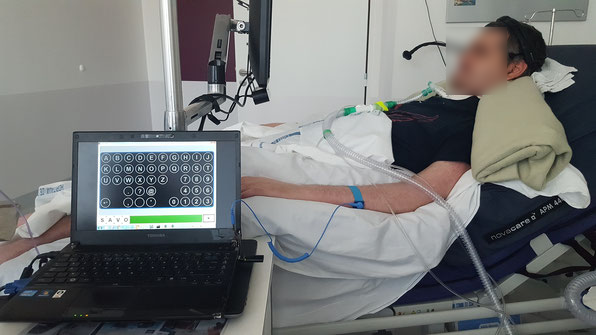
\includegraphics[width=\textwidth]{figures/intro/damien-obfuscated.jpg}
  \end{minipage}\hfill%
  \begin{minipage}[c]{.4\textwidth}
    \raggedright
    Paralysis with impaired speech:
    the \emph{Locked-in Syndrome}
    \bigskip

    Due to
    \begin{itemize}
      \item Stroke
      \item Traumatic brain injury
      \item Neurodegenerative diseases
      \item \ldots
    \end{itemize}
    \bigskip

  Communication requires \\ \emph{assistive technology}
  \bigskip

  What if muscle control is insufficient?
  \end{minipage}
\end{frame}


\note{%
  \begin{itemize}
    \item Some people cannot communicate
    \item Lis:  loss of nearly all voluntary control over muscles.
    \item no speech or typing
    \item require assistive technology
    \item improve QoL
    \item like eye tracker or muscle controlled switch, depending on residual
      control and impairment cannot always use this

    % TODO: Damiens story
  \end{itemize}
}
%
\begin{frame}
  \frametitle{The Brain-Computer Interface}
  \schema{figures/intro/bci.pdf}
\end{frame}


\begin{frame}[c]
  \frametitle{Research question}
  \centering

  \begin{minipage}{.8\textwidth}
  \centering
  \huge
  How can we optimize \emph{BCI}  assistive technology design  to make it more
    \emph{efficient} and  \emph{inclusive}?
  \end{minipage}

\end{frame}

\note{
  inclusive: more people can use it
}



% =============================================================================

\outline{BCI design}{figures/outline_design.pdf}
\outline{BCI design}{figures/outline.pdf}

\begin{frame}[c]
  \frametitle{Recording the brain activity}
  \schema{figures/intro/recording_modalities.pdf}
  \hfill
  \aside{%
    \emph{EEG}  measures the \\ electrical field on the
    scalp:
    \begin{itemize}
      \item[\textcolor{mygreen}{+}] Non-invasive
      \item[\textcolor{mygreen}{+}] Cheap
      \item[\textcolor{myred}{--}] Limited resolution
      \item[\textcolor{myred}{--}] Low signal-to-noise ratio
    \end{itemize}
  }
\end{frame}
% TODO: de clue: we moeten met deze ruis omgaan in paradigm and decoder design


% TODO: je kan de hersenactiviteit wel opnemen, maar dat is pas nuttig als de
% gebruiker een bepaalde taak aan het uitvoeren is zodat we weten welke
% activiteit we eruit moeten halen

\begin{frame}
  \frametitle{BCI paradigms for communication}
  \begin{minipage}[c]{.5\textwidth}
    \footnotesize
    \sffamily
\begin{tikzpicture}[
    scale=\textwidth/3cm,
  ]
  %\useasboundingbox (-1,-1.25) rectangle (1,1);
  \pgfmathsetmacro{\margin}{.1}
  \pgfmathsetmacro{\center}{.5+.5*\margin}
  \pgfmathsetmacro{\textspacing}{.15}
  %\begin{scope}[shift={(1,1.2)}]
    % Draw axes
    \draw[mydarkgray, very thick, <->] ({-(1+\margin)}, 0) -- ({1+\margin},0);
    \draw[mydarkgray, very thick, <->] (0,{-(1+\margin)}) -- (0,{1+\margin});

    % Draw rectangles
    \draw[draw=accent1, fill=white, very thick] ({-\margin}, \margin) rectangle (-1,1);
    \draw[draw=accent2, fill=white, very thick] (\margin, \margin) rectangle (1,1);
    \draw[draw=accent3, fill=white, very thick] (-1, {-\margin}) rectangle (1,-1);

    %% Add text
    \node[color=accent1, align=left,font=\bfseries, anchor=north west, inner sep=2pt] at  (-1,1){active};
    \node[color=accent2, align=left,font=\bfseries, anchor=north east, inner sep=2pt] at  (1,1){reactive};
    \node[color=accent3, align=left,font=\bfseries, anchor=south west, inner sep=2pt] at  (-1,-1){passive};

    \node[color=mydarkgray, align=center,font=\bfseries, anchor=north] at
    (0,{-(1+\margin)}) {passive\\participation};
    \node[color=mydarkgray, align=center,font=\bfseries, anchor=south] at
    (0,{1+\margin}) {active\\participation};
    \node[color=mydarkgray, align=center,font=\bfseries, anchor=east] at ({-(1+\margin)}, 0) {stimulus\\independent};
    \node[color=mydarkgray, align=center,font=\bfseries, anchor=west] at ({1+\margin},0) {stimulus\\dependent};

    %% Text in rectangles
    \node[align=center] at ({-\center}, {\center-\textspacing}) {movement};
    \node[align=center] at ({-\center}, {\center+\textspacing}) {speech};
    %\node[align=center] at ({-\center}, {\center-1.5*\textspacing}) {neurofeedback};

    \node[align=center] at ({\center}, {\center-1.5*\textspacing}) {tactile};
    \node[align=center] at ({\center}, {\center}) {auditory};
    \node[align=center] at ({\center}, {\center+1.5*\textspacing}) {visual};
    %\node[align=center] at ({\center-\textspacing}, {\center-\textspacing}) {mVEP};

    %% More text
    %\node[align=center] at ({\center}, {-\center+\textspacing}) {error\\potentials};
    %\node[align=center] at ({-\center}, {-\center+\textspacing}) {attention and \\ workload detection};
    %\node[align=center] at ({-\center}, {-\center-\textspacing}) {clinical neuroimaging \\ and monitoring};
    %\node[align=center] at ({+\center}, {-\center-\textspacing})  {emotion \\ detection};
    \node[align=center] at (0, {-\center})  {$\cdots$};
  %\end{scope}
\end{tikzpicture}

  \end{minipage}\hfill%

  \aside{%
    \small
    %\emph[accent3]{Passive} BCIs not meant for communication
      \smallskip

      \emph[accent1]{Active} BCIs
      \begin{itemize}
        \footnotesize
        \item[\textcolor{mygreen}{+}] Intuitive, self-paced
        \item[\textcolor{myred}{--}] High speed requires invasive
      \end{itemize}
      \smallskip

      \emph[accent2]{Reactive} BCIs decode reactions to attended stimuli%
      \begin{itemize}
        \footnotesize
        \item[\textcolor{myred}{--}] Less intuitive
        \item[\textcolor{mygreen}{+}] Fast stimulation
        \item[\textcolor{mygreen}{+}] Suited for EEG
      \end{itemize}
      \smallskip

      \emph{Visual reactive} BCIs are a good candidate.
    }
\end{frame}
\note{%
  %TODO: Goal: fast transfering of information in communication assisted technology
  \begin{itemize}
    \item passive BCIs are not meant for communication
    \item categorized participation and stimulation
    \item performing a specific task
    \item brain activity from task can be decoded
  \end{itemize}
}
%TODO: stimuli represent discrete choices, e.g.virtual keyboard

\begin{frame}
  \frametitle{The visual event-related potential  paradigm}
  % TODO: switch bottom top
  \begin{minipage}[c]{.4\textwidth}
    \begin{tikzpicture}
      \node at (current page.north east) [%
        anchor=north east,
        text width=7cm,
        fill=white, opacity=1,
        xshift=1cm,
        yshift=-.5cm,
        thin
      ]{%
        \begin{tikzpicture}[trim axis left]
    \begin{axis}[
        width=\textwidth,
        height=0.6180\textwidth,
        xlabel={Time (ms)},
        ylabel={Potential (uV)},
        axis lines=middle,
        ymin=-5, ymax=10,
        xmin=-100, xmax=800,
        ytick={0}, % Y-ticks at -5, 0, 5
        xtick={0}, % X-ticks at 200, 400, 600, 800
      	ylabel near ticks,
      	xlabel near ticks,
    ]

      % Non-target
      \addplot[
          smooth,
          tension=0.5,
          style={very thick,lightgray},
      ] coordinates {%
          (-100, 0)  % Starting point
          (0, 0)     % Baseline
          (50, 0)    % Pre-P1
          (80, 1)    % P1
          (115, -1)  % N1
          (160, 2)   % P2
          (220, -1)   % N2
          (400, 2)   % P3
          (650, 0)   % LPP (Late Positive Potential)
          (800, 0)   % End point
      };


      % Target
      \addplot[
          smooth,
          tension=0.5,
          style={very thick, accent1}, % Set the line color to accent1
      ] coordinates {%
          (-100, 0)  % Starting point
          (0, 0)     % Baseline
          (50, 0)    % Pre-P1
          (80, 2)    % P1
          (115, -3)  % N1
          (160, 3)   % P2
          (220, 1)   % N2
          (400, 7)   % P3
          (650, 1)   % LPP (Late Positive Potential)
          (800, 1)   % End point
      };

      % Annotations for the components
      \small
      \node[anchor=south, color=muteblack] at (axis cs:80,2) {P1};
      \node[anchor=north, color=muteblack] at (axis cs:115,-3) {N1};
      \node[anchor=south, color=muteblack] at (axis cs:160,3) {P2};
      \node[anchor=west, color=muteblack] at (axis cs:220,1) {N2};
      \node[anchor=south, color=muteblack] at (axis cs:400,7) {P3};
      %\node[anchor=south west, color=muteblack] at (axis cs:650,1) {LPP};

    \end{axis}
\end{tikzpicture}%

      };
    \end{tikzpicture}
    \smallskip

    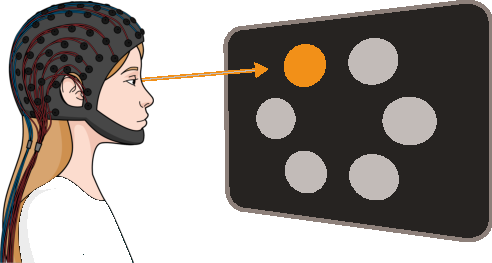
\includegraphics[width=\textwidth]{figures/intro/oddball.pdf}
  \end{minipage}\hfill%
  \begin{minipage}[c]{.5\textwidth}
    \begin{enumerate}
      \item Stimuli flash one by one
      \smallskip
      \item Flashes evoke ERPs
      \smallskip
      \item User attends a stimulus
      \smallskip
      \item ERP components are \\ modulated by attention
      \smallskip
      \item Decode target based on \\ timing and components
    \end{enumerate}
  \end{minipage}
\end{frame}


% =============================================================================

\outline{\emph{C1.} Spatiotemporal ERP decoding}{figures/outline_decode.pdf}
\begin{frame}[c]
  \frametitle{\emph{Problem:} ERP responses can be difficult to extract}
  \begin{minipage}[c]{.5\textwidth}

    Low single-trial signal-to-noise ratio
    \begin{itemize}
      \item Machine learning models must be \\ trained to decode ERPs
    \end{itemize}
    \bigskip

    Each response is a sample with \\
    \# features $=$ \# channels $\times$ \# time points
    \begin{itemize}
      \item High number of features \\ (channels $\times$ times)
      \item Short calibration time \\ results in low sample size
    \end{itemize}
    \bigskip

    \centering
    \emph{\# features $>>$ \# samples}

  \end{minipage}\hfill%
  \begin{minipage}[c]{.4\textwidth}
    \raggedleft

    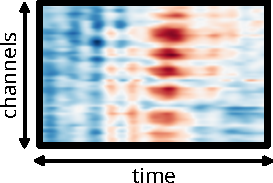
\includegraphics[width=\textwidth]{figures/bttda/tensor_st.pdf}

  \end{minipage}
\end{frame}

\begin{frame}[c]
  \frametitle{Retaining space-time structure enhances performance}
  \bigskip

  \begin{minipage}[c]{.5\textwidth}
    Data are ususally flattened \\ before classification
    \begin{itemize}
      \item   ignores channel-time point structure
    \end{itemize}
  \end{minipage}\hfill%
  \begin{minipage}[c]{.4\textwidth}
    \vfill
    \raggedleft
    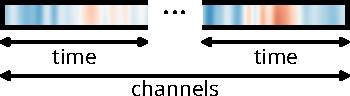
\includegraphics[width=.9\textwidth]{figures/bttda/tensor_flat.pdf}
  \end{minipage}
  \bigskip
  \bigskip

  \begin{minipage}[c]{.5\textwidth}
    Assumptions on \emph{data structure}
    \begin{itemize}
      \item yield strong regularization
      \item speed up training
    \end{itemize}
  \end{minipage}\hfill%
  \begin{minipage}[c]{.4\textwidth}
    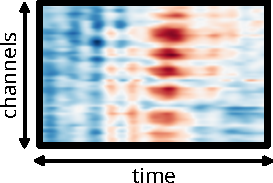
\includegraphics[width=\textwidth]{figures/bttda/tensor_st.pdf}
  \end{minipage}

\end{frame}

\begin{frame}[c]
  \frametitle{Covariance matrix regularization \\
  {\tiny\cite{VanDenKerchove2022}}}
  \begin{minipage}[c]{.3\textwidth}
  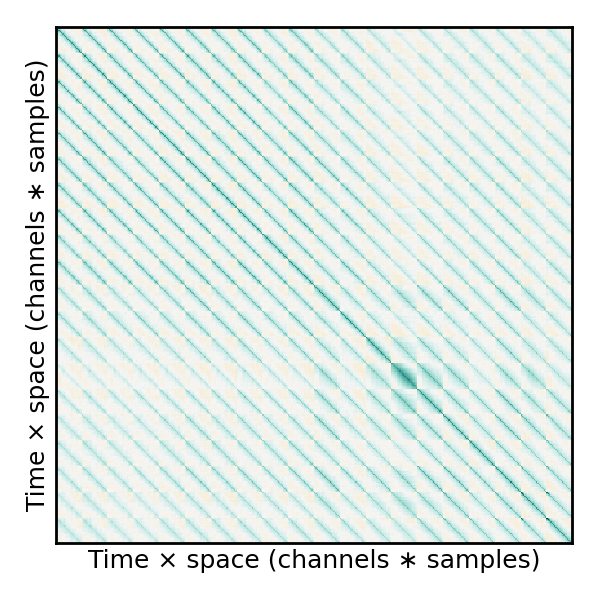
\includegraphics[width=\textwidth]{figures/decode/emp_cov_label.png}
  \end{minipage}
  $=$
  \begin{minipage}[c]{.3\textwidth}
    \begin{minipage}[c]{.4\textwidth}
      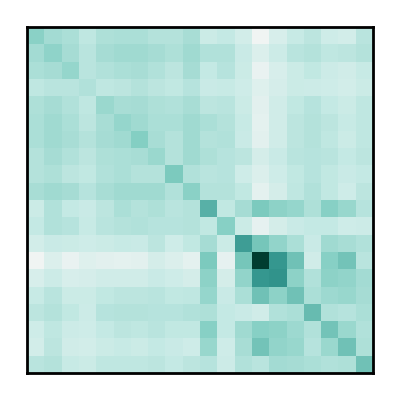
\includegraphics[width=\textwidth]{figures/decode/sp_cov_2.png}
    \end{minipage}
  $\otimes$
    \begin{minipage}[c]{.4\textwidth}
      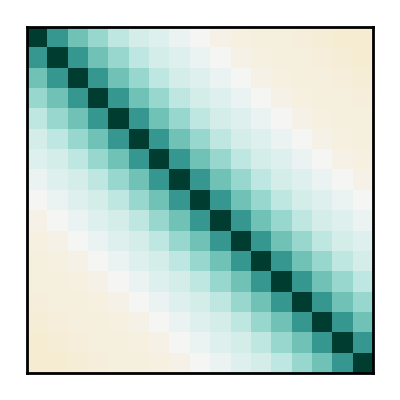
\includegraphics[width=\textwidth]{figures/decode/tmp_cov_2.png}
    \end{minipage}
  \end{minipage}\hfill
  \aside{
    Linear decoders require covariance estimation and inversion
    \bigskip

    Imprecise due to high dimensionality
    \bigskip

    Repetitive structure can be expressed as separate space and
    time covariance
    \bigskip

    Saves computation time and improves accuracy for low data
    availability



  }


\end{frame}

\begin{frame}
  \frametitle{Tensor feature extraction {\tiny\cite{VanDenKerchovesubmitted}}}

  \begin{minipage}[t]{.35\linewidth}
    Tensor discriminant analysis
    \bigskip

		\centering
		\begin{tikzpicture}[y=-1cm]
			\begin{scope}[shift={(-1,0)}]
        \TensorThree{$\ten{X}$}{\rotatebox{90}{\small channels}}{\small times}{}{2}{2}{1}
				\node at (3.2,.5, 2) {$\rightarrow$};
				\begin{scope}[shift={(3.25,0.25)}]
					\TensorThree{$\ten{G}$}{}{}{}{1}{1}{1}
				\end{scope}
				\node at (4.2,1.25, 2) {$\downarrow$};
				\begin{scope}[shift={(3,2)}]
					\TensorTwo{\textit{clf}}{}{}{1.5}{.5}
				\end{scope}
			\end{scope}
    \end{tikzpicture}
    {\tiny\cite{Phan2010}}
	\end{minipage}\hfill%
  \vrule\hfill%
  \begin{minipage}[t]{.55\textwidth}
    Block-term tensor discriminant analysis
    \bigskip

    \centering
		\begin{tikzpicture}[y=-1cm]
			\begin{scope}[shift={(-1,0)}]
				\TensorThree{$\ten{X}$}{}{}{}{2}{2}{1}
				\node at (3.2,.5, 2) {$\rightarrow$};
				\begin{scope}[shift={(3.25,0.25)}]
					\TensorThree{$\ten{G}^{(1)}$}{}{}{}{1}{1}{1}
				\end{scope}
				\node at (5.75,.5,2) {$,\cdots,$};
				\begin{scope}[shift={(6.25,0.25)}]
					\TensorThree{$\ten{G}^{(B)}$}{}{}{}{1}{1}{1}
				\end{scope}
				\node at (4.2,1.25, 2) {$\downarrow$};
				\node at (5.7,1.25, 2) {$\downarrow$};
				\node at (7.2,1.25, 2) {$\downarrow$};
				\begin{scope}[shift={(3,2)}]
					\TensorTwo{\textit{clf}}{}{}{4.5}{.5}
				\end{scope}
			\end{scope}
    \end{tikzpicture}
    \smallskip

    \begin{minipage}[t]{.5\textwidth}
      \small
      \posi\ \ More flexible
      \smallskip

      \posi\ \ Retains structure
    \end{minipage}\hfill%
    \begin{minipage}[t]{.5\textwidth}
      \small\raggedright
      \nega\ \ More parameters
      \smallskip

      Heuristic model selection
      \smallskip

      Validated with 4 open datasets
    \end{minipage}
  \end{minipage}

\end{frame}
\note{
  Another method: consider that we keep all data in its original shape and find
  separate transformations for space and for time
}


% =============================================================================

\outline{\emph{C2.} Gaze-independence}{figures/outline_gaze.pdf}


\begin{frame}
  \frametitle{\emph{Problem:} Eye motor impairment \\  prevents gazing at targets}

  \begin{minipage}[c]{.4\textwidth}
    \raggedright
    \emph{Visual skills} related to disease \\ affect BCI
    operation
    {\tiny\cite{FriedOken2020}}
  {\small
  \begin{itemize}
    \item Discomfort fixating
    \item Restricted movement
    \item Involuntary movements
  \end{itemize}
  }
  \bigskip

  Decoding relies on \emph{visual ERP} components {\tiny\cite{Treder2010}}
	\end{minipage}\hfill%
  \begin{minipage}[c]{.4\textwidth}
		\centering
		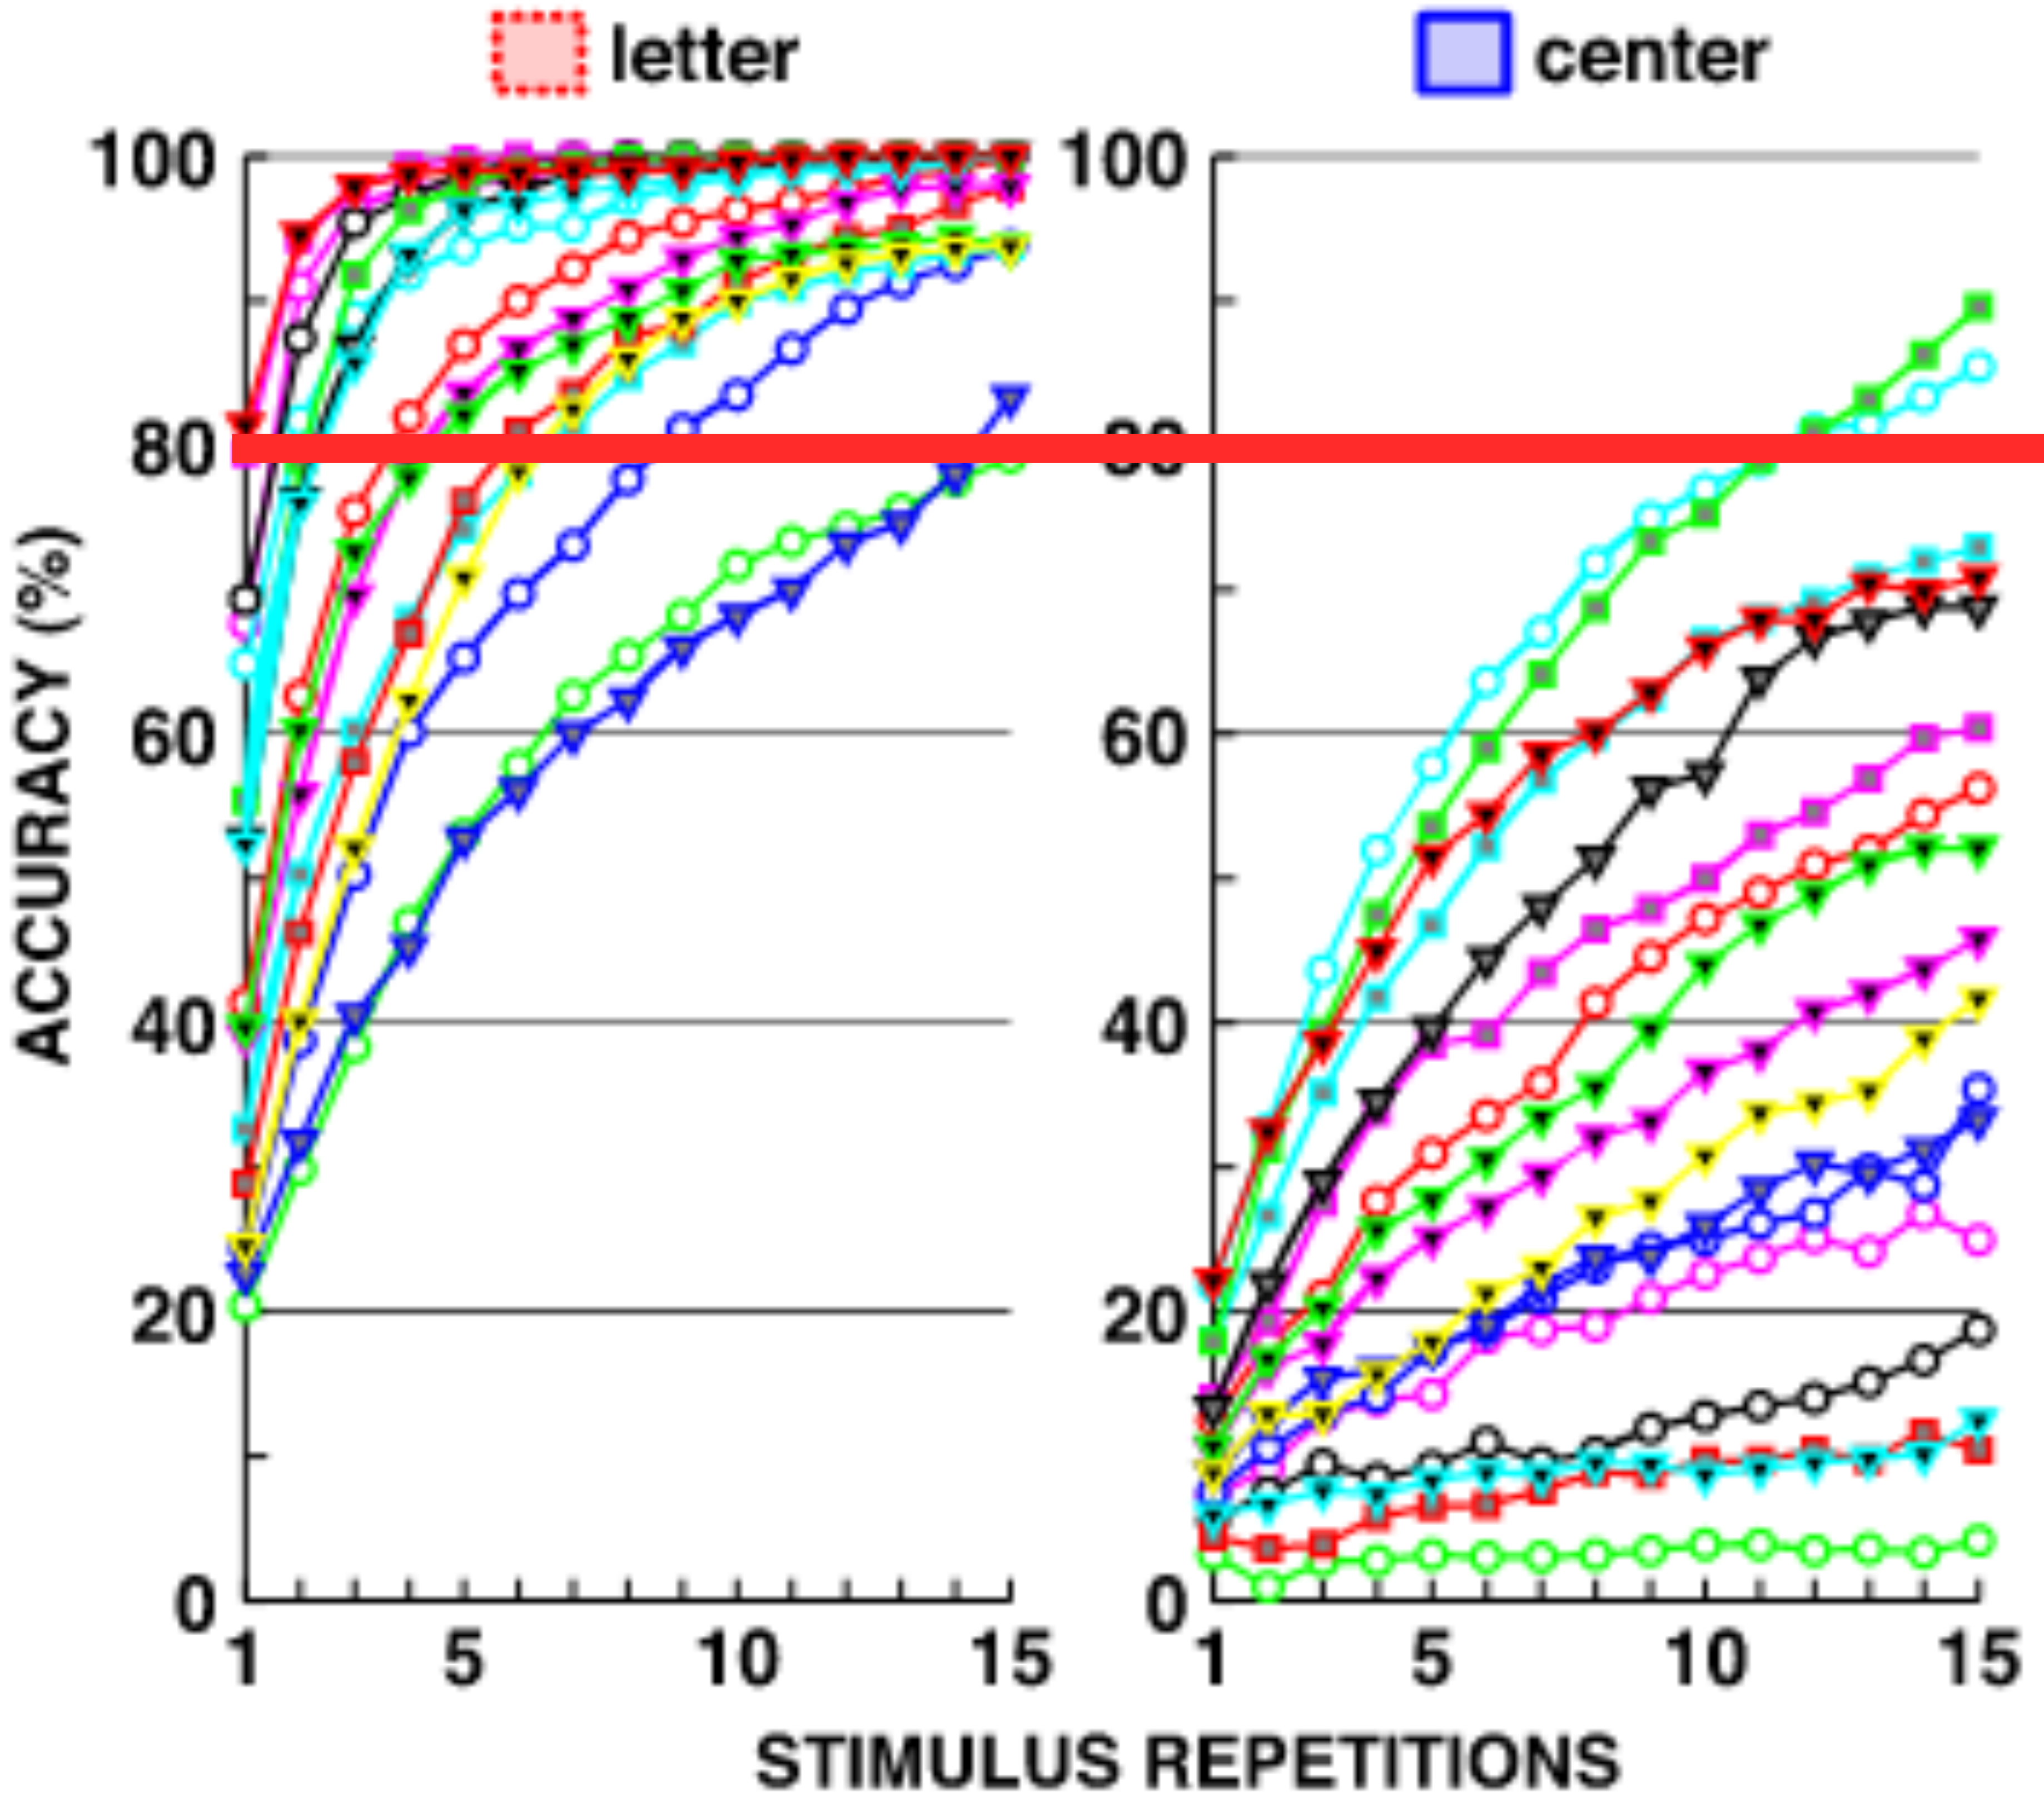
\includegraphics[width=\textwidth]{figures/intro/covert_performance_drop/brunner_2010_line.png}

    {\tiny\cite{RonAngevin2019}}


	\end{minipage}
\end{frame}

\note{
  \begin{itemize}
    \item Explain axes
    \item Accuracy is lower when not gazing directly
    \item Even below 80\% usability threshold
  \end{itemize}

}


\begin{frame}
  \frametitle{Covert visuospatial attention experiment}

  \begin{minipage}{.6\textwidth}
    \centering

    \begin{minipage}[t]{.45\textwidth}
    \begin{tikzpicture}[
    scale=\textwidth/5cm
]
% Rectangle background
\fill[muteblack] (-2.5,-2) rectangle (2.5,2);

% Hexagon vertices (white circles)
\fill[white] (1,0) circle (.35);    % Right
\fill[white] (-1,0) circle (.35);   % Left
\fill[white] (0.5,0.866) circle (.35); % Top-right
\fill[white] (-0.5,0.866) circle (.35); % Top-left
\fill[white] (0.5,-0.866) circle (.35); % Bottom-right
\fill[white] (-0.5,-0.866) circle (.35); % Bottom-left
\draw[accent2, ultra thick] (0.9,0) -- (1.1,0);  % Shorter horizontal line
\draw[accent2, ultra thick] (1,-0.1) -- (1,0.1); % Shorter vertical line
\end{tikzpicture}%

    \end{minipage}\hfill%
    \begin{minipage}[t]{.45\textwidth}
      \includegraphics[width=\textwidth]{example-image}

      timeline
    \end{minipage}
    \bigskip
    \bigskip
    \bigskip


    {\small
    \begin{minipage}{.3\textwidth}
      Overt VSA
      \smallskip

      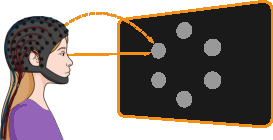
\includegraphics[width=\textwidth]{figures/covert/attention_overt.pdf}
    \end{minipage}\hfill%
    \begin{minipage}{.3\textwidth}
      Covert VSA
      \smallskip

      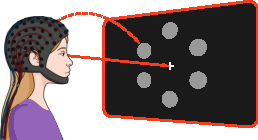
\includegraphics[width=\textwidth]{figures/covert/attention_covert.pdf}
    \end{minipage}\hfill%
    \begin{minipage}{.3\textwidth}
      \small
      Split VSA
      \smallskip

      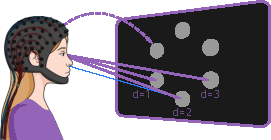
\includegraphics[width=\textwidth]{figures/covert/attention_split.pdf}
    \end{minipage}%
  }
  \end{minipage}\hfill

  \aside{%
    \small
    \raggedright
    CVSA-ERP dataset
    \begin{itemize}
      \item 15 subjects, $\pm$ 11h stimulation
      \item Hex-o-Spell interface \\ {\tiny\cite{Treder2010}}
      \item Discrete gaze-\\independence conditions
    \end{itemize}
    \raggedright
    {\tiny\cite{VanDenKerchove2024}}
  }
\end{frame}
\note{
  Hex-o-Spell optimized for gaze-independence
}

\begin{frame}
  \frametitle{Evoked ERP components}
  \small
  \begin{minipage}[t]{.45\textwidth}
    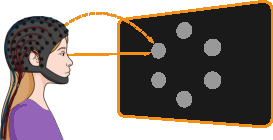
\includegraphics[width=.2\textwidth]{figures/covert/attention_overt.pdf}
    \hspace{.5em}
    \emph{Overt} VSA
    \smallskip

    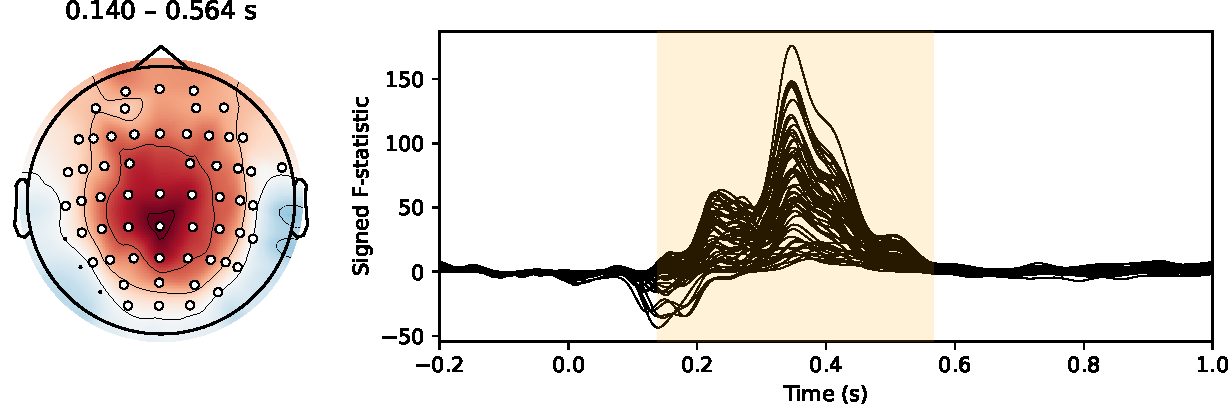
\includegraphics[width=\textwidth]{figures/covert/erps/erp_overt_cluster-1.pdf}
    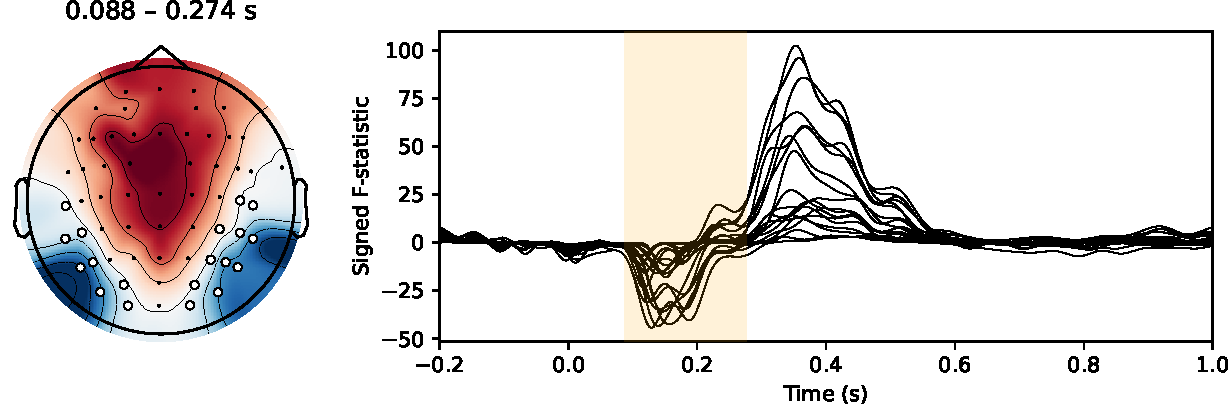
\includegraphics[width=\textwidth]{figures/covert/erps/erp_overt_cluster-0.pdf}
    \smallskip

    \small
    F-statistic cluster-based permutation \\ tests, target vs. non-target
  \end{minipage}\hfill%
  \begin{minipage}[t]{.45\textwidth}
    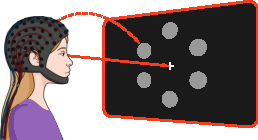
\includegraphics[width=.2\textwidth]{figures/covert/attention_covert.pdf}
    \hspace{.5em}
    \emph{Covert} VSA
    \smallskip

    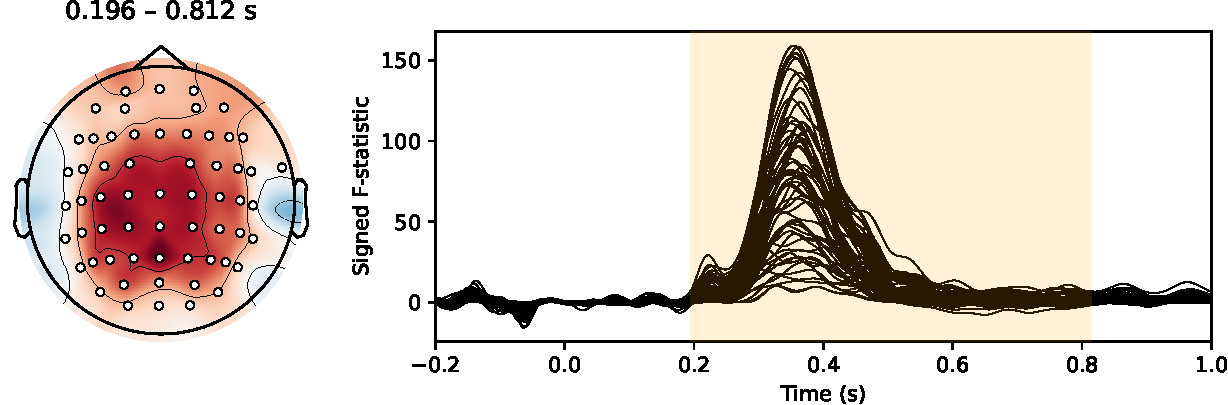
\includegraphics[width=\textwidth]{figures/covert/erps/erp_covert_cluster-0.pdf}
    \smallskip

    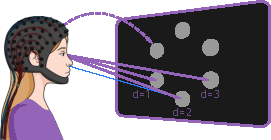
\includegraphics[width=.2\textwidth]{figures/covert/attention_split.pdf}
    \hspace{.5em}
    \emph{Split} VSA
    \smallskip

    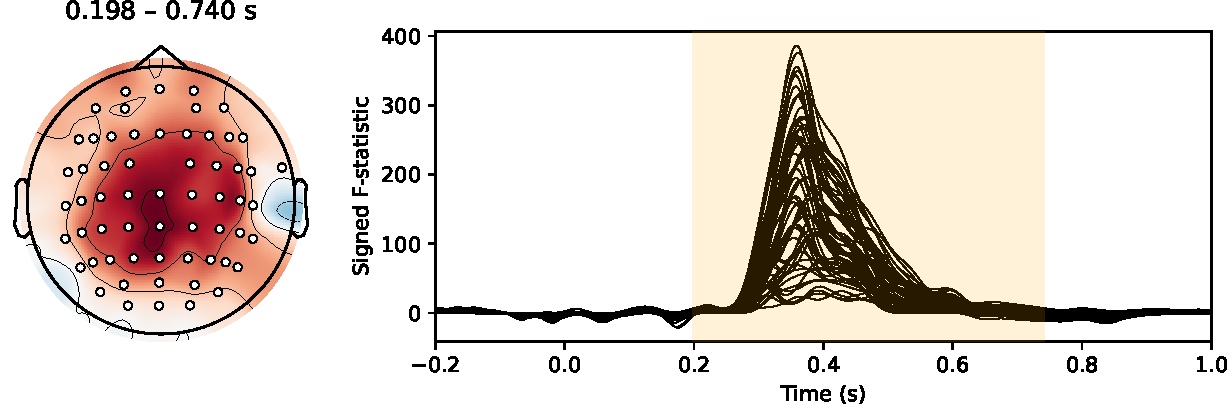
\includegraphics[width=\textwidth]{figures/covert/erps/erp_split_cluster-0.pdf}

  \end{minipage}
\end{frame}


%% =============================================================================

\outline{\emph{C3.} Gaze-independent decoding}{figures/outline_decode.pdf}

\begin{frame}[c]
  \frametitle{\emph{Problem:} Latency jitter decreases performance \\ in covert and split
  attention}
  \begin{minipage}{.4\textwidth}
    \centering
\small

\begin{tikzpicture}   % First subplot (low jitter) positioned relative to center
    \begin{axis}[
        at={(0,0)}, % Adjust position to the left, closer to the center
        anchor=center,
        width=\textwidth, height=.7\textwidth,
        xmin=20, xmax=80,
        ymin=-0.1, ymax=1.1,
        axis lines=none, % Remove axes
        title={low jitter}, % Add title
        title style={yshift=-10pt, color=muteblack}, % Adjust title position to make it closer to the plot
        ]
        % Plot individual waveforms (low jitter) in darkgray
        \addplot[darkgray,domain=20:80,samples=100] {exp(-0.5*((x-50)/5)^2)};
        \addplot[darkgray,domain=20:80,samples=100] {exp(-0.5*((x-52)/5)^2)};
        \addplot[darkgray,domain=20:80,samples=100] {exp(-0.5*((x-48)/5)^2)};
        \addplot[darkgray,domain=20:80,samples=100] {exp(-0.5*((x-51)/5)^2)};
        \addplot[darkgray,domain=20:80,samples=100] {exp(-0.5*((x-49)/5)^2)};

        % Plot average waveform (low jitter) in accent1 color, very thick
        \addplot[ultra thick,accent1,domain=20:80,samples=100] {exp(-0.5*((x-50)/5)^2)};
    \end{axis}
\end{tikzpicture}
\bigskip

\begin{tikzpicture}

   % Second subplot (high jitter) positioned relative to center
   \begin{axis}[
      at={(0.55\textwidth,0)}, % Adjust position to the left, closer to the center
       anchor=center,
        width=\textwidth, height=.7\textwidth,
       xmin=20, xmax=80,
       ymin=-0.1, ymax=1.1,
       axis lines=none, % Remove axes
       title={high jitter}, % Add title
       title style={yshift=-10pt, color=muteblack}, % Adjust title position to make it closer to the plot
       ]
       % Plot individual waveforms (high jitter) in darkgray
       \addplot[darkgray,domain=20:80,samples=100] {exp(-0.5*((x-45)/5)^2)};
       \addplot[darkgray,domain=20:80,samples=100] {exp(-0.5*((x-55)/5)^2)};
       \addplot[darkgray,domain=20:80,samples=100] {exp(-0.5*((x-40)/5)^2)};
       \addplot[darkgray,domain=20:80,samples=100] {exp(-0.5*((x-60)/5)^2)};
       \addplot[darkgray,domain=20:80,samples=100] {exp(-0.5*((x-50)/5)^2)};

       % Plot average waveform (high jitter) in accent1 color, very thick
       \addplot[ultra thick,accent1,domain=20:80,samples=100] {0.2*(exp(-0.5*((x-45)/5)^2) + exp(-0.5*((x-55)/5)^2) + exp(-0.5*((x-40)/5)^2) + exp(-0.5*((x-60)/5)^2) + exp(-0.5*((x-50)/5)^2))};
   \end{axis}
\end{tikzpicture}%
\bigskip

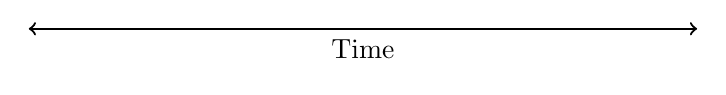
\begin{tikzpicture}
    % Draw the bottom horizontal axis
    \draw[thick,<->] (-0.35\textwidth,-1) -- (.35\textwidth,-1) node[pos=0.5,below] {Time};
\end{tikzpicture}
%\vspace{-5cm}

  \end{minipage}\hfill%
  \begin{minipage}{.55\textwidth}
    \small
    \centering
    {\centering\resizebox{.7\textwidth}{!}{%
    \small
    %CVSA-ERP (our dataset) \hspace{3.5em} BNCI2014-009
    %\smallskip

    \hspace{-0.24572736754045163in}
%%% Creator: Matplotlib, PGF backend
%%
%% To include the figure in your LaTeX document, write
%%   \input{<filename>.pgf}
%%
%% Make sure the required packages are loaded in your preamble
%%   \usepackage{pgf}
%%
%% Also ensure that all the required font packages are loaded; for instance,
%% the lmodern package is sometimes necessary when using math font.
%%   \usepackage{lmodern}
%%
%% Figures using additional raster images can only be included by \input if
%% they are in the same directory as the main LaTeX file. For loading figures
%% from other directories you can use the `import` package
%%   \usepackage{import}
%%
%% and then include the figures with
%%   \import{<path to file>}{<filename>.pgf}
%%
%% Matplotlib used the following preamble
%%   \def\mathdefault#1{#1}
%%   \everymath=\expandafter{\the\everymath\displaystyle}
%%
%%   \ifdefined\pdftexversion\else  % non-pdftex case.
%%     \usepackage{fontspec}
%%   \fi
%%   \makeatletter\@ifpackageloaded{underscore}{}{\usepackage[strings]{underscore}}\makeatother
%%
\begingroup%
\makeatletter%
\begin{pgfpicture}%
\pgfpathrectangle{\pgfpointorigin}{\pgfqpoint{2.997033in}{1.668849in}}%
\pgfusepath{use as bounding box, clip}%
\begin{pgfscope}%
\pgfsetbuttcap%
\pgfsetmiterjoin%
\pgfsetlinewidth{0.000000pt}%
\definecolor{currentstroke}{rgb}{1.000000,1.000000,1.000000}%
\pgfsetstrokecolor{currentstroke}%
\pgfsetstrokeopacity{0.000000}%
\pgfsetdash{}{0pt}%
\pgfpathmoveto{\pgfqpoint{0.000000in}{0.000000in}}%
\pgfpathlineto{\pgfqpoint{2.997033in}{0.000000in}}%
\pgfpathlineto{\pgfqpoint{2.997033in}{1.668849in}}%
\pgfpathlineto{\pgfqpoint{0.000000in}{1.668849in}}%
\pgfpathlineto{\pgfqpoint{0.000000in}{0.000000in}}%
\pgfpathclose%
\pgfusepath{}%
\end{pgfscope}%
\begin{pgfscope}%
\pgfsetbuttcap%
\pgfsetmiterjoin%
\definecolor{currentfill}{rgb}{1.000000,1.000000,1.000000}%
\pgfsetfillcolor{currentfill}%
\pgfsetlinewidth{0.000000pt}%
\definecolor{currentstroke}{rgb}{0.000000,0.000000,0.000000}%
\pgfsetstrokecolor{currentstroke}%
\pgfsetstrokeopacity{0.000000}%
\pgfsetdash{}{0pt}%
\pgfpathmoveto{\pgfqpoint{0.229167in}{0.470139in}}%
\pgfpathlineto{\pgfqpoint{2.146685in}{0.470139in}}%
\pgfpathlineto{\pgfqpoint{2.146685in}{1.608911in}}%
\pgfpathlineto{\pgfqpoint{0.229167in}{1.608911in}}%
\pgfpathlineto{\pgfqpoint{0.229167in}{0.470139in}}%
\pgfpathclose%
\pgfusepath{fill}%
\end{pgfscope}%
\begin{pgfscope}%
\pgfpathrectangle{\pgfqpoint{0.229167in}{0.470139in}}{\pgfqpoint{1.917519in}{1.138772in}}%
\pgfusepath{clip}%
\pgfsetbuttcap%
\pgfsetmiterjoin%
\definecolor{currentfill}{rgb}{0.842157,0.553922,0.200980}%
\pgfsetfillcolor{currentfill}%
\pgfsetlinewidth{0.000000pt}%
\definecolor{currentstroke}{rgb}{0.000000,0.000000,0.000000}%
\pgfsetstrokecolor{currentstroke}%
\pgfsetstrokeopacity{0.000000}%
\pgfsetdash{}{0pt}%
\pgfpathmoveto{\pgfqpoint{0.316327in}{0.470139in}}%
\pgfpathlineto{\pgfqpoint{0.606860in}{0.470139in}}%
\pgfpathlineto{\pgfqpoint{0.606860in}{0.705246in}}%
\pgfpathlineto{\pgfqpoint{0.316327in}{0.705246in}}%
\pgfpathlineto{\pgfqpoint{0.316327in}{0.470139in}}%
\pgfpathclose%
\pgfusepath{fill}%
\end{pgfscope}%
\begin{pgfscope}%
\pgfpathrectangle{\pgfqpoint{0.229167in}{0.470139in}}{\pgfqpoint{1.917519in}{1.138772in}}%
\pgfusepath{clip}%
\pgfsetbuttcap%
\pgfsetmiterjoin%
\definecolor{currentfill}{rgb}{0.858824,0.314706,0.223529}%
\pgfsetfillcolor{currentfill}%
\pgfsetlinewidth{0.000000pt}%
\definecolor{currentstroke}{rgb}{0.000000,0.000000,0.000000}%
\pgfsetstrokecolor{currentstroke}%
\pgfsetstrokeopacity{0.000000}%
\pgfsetdash{}{0pt}%
\pgfpathmoveto{\pgfqpoint{0.679493in}{0.470139in}}%
\pgfpathlineto{\pgfqpoint{0.970026in}{0.470139in}}%
\pgfpathlineto{\pgfqpoint{0.970026in}{1.007696in}}%
\pgfpathlineto{\pgfqpoint{0.679493in}{1.007696in}}%
\pgfpathlineto{\pgfqpoint{0.679493in}{0.470139in}}%
\pgfpathclose%
\pgfusepath{fill}%
\end{pgfscope}%
\begin{pgfscope}%
\pgfpathrectangle{\pgfqpoint{0.229167in}{0.470139in}}{\pgfqpoint{1.917519in}{1.138772in}}%
\pgfusepath{clip}%
\pgfsetbuttcap%
\pgfsetmiterjoin%
\definecolor{currentfill}{rgb}{0.464706,0.320588,0.573529}%
\pgfsetfillcolor{currentfill}%
\pgfsetlinewidth{0.000000pt}%
\definecolor{currentstroke}{rgb}{0.000000,0.000000,0.000000}%
\pgfsetstrokecolor{currentstroke}%
\pgfsetstrokeopacity{0.000000}%
\pgfsetdash{}{0pt}%
\pgfpathmoveto{\pgfqpoint{1.042660in}{0.470139in}}%
\pgfpathlineto{\pgfqpoint{1.333193in}{0.470139in}}%
\pgfpathlineto{\pgfqpoint{1.333193in}{0.979341in}}%
\pgfpathlineto{\pgfqpoint{1.042660in}{0.979341in}}%
\pgfpathlineto{\pgfqpoint{1.042660in}{0.470139in}}%
\pgfpathclose%
\pgfusepath{fill}%
\end{pgfscope}%
\begin{pgfscope}%
\pgfpathrectangle{\pgfqpoint{0.229167in}{0.470139in}}{\pgfqpoint{1.917519in}{1.138772in}}%
\pgfusepath{clip}%
\pgfsetbuttcap%
\pgfsetmiterjoin%
\definecolor{currentfill}{rgb}{0.464706,0.320588,0.573529}%
\pgfsetfillcolor{currentfill}%
\pgfsetlinewidth{0.000000pt}%
\definecolor{currentstroke}{rgb}{0.000000,0.000000,0.000000}%
\pgfsetstrokecolor{currentstroke}%
\pgfsetstrokeopacity{0.000000}%
\pgfsetdash{}{0pt}%
\pgfpathmoveto{\pgfqpoint{1.405826in}{0.470139in}}%
\pgfpathlineto{\pgfqpoint{1.696359in}{0.470139in}}%
\pgfpathlineto{\pgfqpoint{1.696359in}{1.012421in}}%
\pgfpathlineto{\pgfqpoint{1.405826in}{1.012421in}}%
\pgfpathlineto{\pgfqpoint{1.405826in}{0.470139in}}%
\pgfpathclose%
\pgfusepath{fill}%
\end{pgfscope}%
\begin{pgfscope}%
\pgfpathrectangle{\pgfqpoint{0.229167in}{0.470139in}}{\pgfqpoint{1.917519in}{1.138772in}}%
\pgfusepath{clip}%
\pgfsetbuttcap%
\pgfsetmiterjoin%
\definecolor{currentfill}{rgb}{0.464706,0.320588,0.573529}%
\pgfsetfillcolor{currentfill}%
\pgfsetlinewidth{0.000000pt}%
\definecolor{currentstroke}{rgb}{0.000000,0.000000,0.000000}%
\pgfsetstrokecolor{currentstroke}%
\pgfsetstrokeopacity{0.000000}%
\pgfsetdash{}{0pt}%
\pgfpathmoveto{\pgfqpoint{1.768992in}{0.470139in}}%
\pgfpathlineto{\pgfqpoint{2.059526in}{0.470139in}}%
\pgfpathlineto{\pgfqpoint{2.059526in}{0.975797in}}%
\pgfpathlineto{\pgfqpoint{1.768992in}{0.975797in}}%
\pgfpathlineto{\pgfqpoint{1.768992in}{0.470139in}}%
\pgfpathclose%
\pgfusepath{fill}%
\end{pgfscope}%
\begin{pgfscope}%
\pgfsetbuttcap%
\pgfsetroundjoin%
\definecolor{currentfill}{rgb}{0.552941,0.501961,0.478431}%
\pgfsetfillcolor{currentfill}%
\pgfsetlinewidth{0.803000pt}%
\definecolor{currentstroke}{rgb}{0.552941,0.501961,0.478431}%
\pgfsetstrokecolor{currentstroke}%
\pgfsetdash{}{0pt}%
\pgfsys@defobject{currentmarker}{\pgfqpoint{0.000000in}{0.000000in}}{\pgfqpoint{0.000000in}{0.041667in}}{%
\pgfpathmoveto{\pgfqpoint{0.000000in}{0.000000in}}%
\pgfpathlineto{\pgfqpoint{0.000000in}{0.041667in}}%
\pgfusepath{stroke,fill}%
}%
\begin{pgfscope}%
\pgfsys@transformshift{0.461593in}{0.470139in}%
\pgfsys@useobject{currentmarker}{}%
\end{pgfscope}%
\end{pgfscope}%
\begin{pgfscope}%
\definecolor{textcolor}{rgb}{0.552941,0.501961,0.478431}%
\pgfsetstrokecolor{textcolor}%
\pgfsetfillcolor{textcolor}%
\pgftext[x=0.461593in,y=0.421528in,,top]{\color{textcolor}{\sffamily\fontsize{9.000000}{10.800000}\selectfont\catcode`\^=\active\def^{\ifmmode\sp\else\^{}\fi}\catcode`\%=\active\def%{\%}overt}}%
\end{pgfscope}%
\begin{pgfscope}%
\pgfsetbuttcap%
\pgfsetroundjoin%
\definecolor{currentfill}{rgb}{0.552941,0.501961,0.478431}%
\pgfsetfillcolor{currentfill}%
\pgfsetlinewidth{0.803000pt}%
\definecolor{currentstroke}{rgb}{0.552941,0.501961,0.478431}%
\pgfsetstrokecolor{currentstroke}%
\pgfsetdash{}{0pt}%
\pgfsys@defobject{currentmarker}{\pgfqpoint{0.000000in}{0.000000in}}{\pgfqpoint{0.000000in}{0.041667in}}{%
\pgfpathmoveto{\pgfqpoint{0.000000in}{0.000000in}}%
\pgfpathlineto{\pgfqpoint{0.000000in}{0.041667in}}%
\pgfusepath{stroke,fill}%
}%
\begin{pgfscope}%
\pgfsys@transformshift{0.824760in}{0.470139in}%
\pgfsys@useobject{currentmarker}{}%
\end{pgfscope}%
\end{pgfscope}%
\begin{pgfscope}%
\definecolor{textcolor}{rgb}{0.552941,0.501961,0.478431}%
\pgfsetstrokecolor{textcolor}%
\pgfsetfillcolor{textcolor}%
\pgftext[x=0.824760in,y=0.421528in,,top]{\color{textcolor}{\sffamily\fontsize{9.000000}{10.800000}\selectfont\catcode`\^=\active\def^{\ifmmode\sp\else\^{}\fi}\catcode`\%=\active\def%{\%}covert}}%
\end{pgfscope}%
\begin{pgfscope}%
\pgfsetbuttcap%
\pgfsetroundjoin%
\definecolor{currentfill}{rgb}{0.552941,0.501961,0.478431}%
\pgfsetfillcolor{currentfill}%
\pgfsetlinewidth{0.803000pt}%
\definecolor{currentstroke}{rgb}{0.552941,0.501961,0.478431}%
\pgfsetstrokecolor{currentstroke}%
\pgfsetdash{}{0pt}%
\pgfsys@defobject{currentmarker}{\pgfqpoint{0.000000in}{0.000000in}}{\pgfqpoint{0.000000in}{0.041667in}}{%
\pgfpathmoveto{\pgfqpoint{0.000000in}{0.000000in}}%
\pgfpathlineto{\pgfqpoint{0.000000in}{0.041667in}}%
\pgfusepath{stroke,fill}%
}%
\begin{pgfscope}%
\pgfsys@transformshift{1.187926in}{0.470139in}%
\pgfsys@useobject{currentmarker}{}%
\end{pgfscope}%
\end{pgfscope}%
\begin{pgfscope}%
\definecolor{textcolor}{rgb}{0.552941,0.501961,0.478431}%
\pgfsetstrokecolor{textcolor}%
\pgfsetfillcolor{textcolor}%
\pgftext[x=1.076257in, y=0.334722in, left, base]{\color{textcolor}{\sffamily\fontsize{9.000000}{10.800000}\selectfont\catcode`\^=\active\def^{\ifmmode\sp\else\^{}\fi}\catcode`\%=\active\def%{\%}split}}%
\end{pgfscope}%
\begin{pgfscope}%
\definecolor{textcolor}{rgb}{0.552941,0.501961,0.478431}%
\pgfsetstrokecolor{textcolor}%
\pgfsetfillcolor{textcolor}%
\pgftext[x=0.986917in, y=0.197917in, left, base]{\color{textcolor}{\sffamily\fontsize{9.000000}{10.800000}\selectfont\catcode`\^=\active\def^{\ifmmode\sp\else\^{}\fi}\catcode`\%=\active\def%{\%}($d=1$)}}%
\end{pgfscope}%
\begin{pgfscope}%
\pgfsetbuttcap%
\pgfsetroundjoin%
\definecolor{currentfill}{rgb}{0.552941,0.501961,0.478431}%
\pgfsetfillcolor{currentfill}%
\pgfsetlinewidth{0.803000pt}%
\definecolor{currentstroke}{rgb}{0.552941,0.501961,0.478431}%
\pgfsetstrokecolor{currentstroke}%
\pgfsetdash{}{0pt}%
\pgfsys@defobject{currentmarker}{\pgfqpoint{0.000000in}{0.000000in}}{\pgfqpoint{0.000000in}{0.041667in}}{%
\pgfpathmoveto{\pgfqpoint{0.000000in}{0.000000in}}%
\pgfpathlineto{\pgfqpoint{0.000000in}{0.041667in}}%
\pgfusepath{stroke,fill}%
}%
\begin{pgfscope}%
\pgfsys@transformshift{1.551093in}{0.470139in}%
\pgfsys@useobject{currentmarker}{}%
\end{pgfscope}%
\end{pgfscope}%
\begin{pgfscope}%
\definecolor{textcolor}{rgb}{0.552941,0.501961,0.478431}%
\pgfsetstrokecolor{textcolor}%
\pgfsetfillcolor{textcolor}%
\pgftext[x=1.439423in, y=0.334722in, left, base]{\color{textcolor}{\sffamily\fontsize{9.000000}{10.800000}\selectfont\catcode`\^=\active\def^{\ifmmode\sp\else\^{}\fi}\catcode`\%=\active\def%{\%}split}}%
\end{pgfscope}%
\begin{pgfscope}%
\definecolor{textcolor}{rgb}{0.552941,0.501961,0.478431}%
\pgfsetstrokecolor{textcolor}%
\pgfsetfillcolor{textcolor}%
\pgftext[x=1.350083in, y=0.197917in, left, base]{\color{textcolor}{\sffamily\fontsize{9.000000}{10.800000}\selectfont\catcode`\^=\active\def^{\ifmmode\sp\else\^{}\fi}\catcode`\%=\active\def%{\%}($d=2$)}}%
\end{pgfscope}%
\begin{pgfscope}%
\pgfsetbuttcap%
\pgfsetroundjoin%
\definecolor{currentfill}{rgb}{0.552941,0.501961,0.478431}%
\pgfsetfillcolor{currentfill}%
\pgfsetlinewidth{0.803000pt}%
\definecolor{currentstroke}{rgb}{0.552941,0.501961,0.478431}%
\pgfsetstrokecolor{currentstroke}%
\pgfsetdash{}{0pt}%
\pgfsys@defobject{currentmarker}{\pgfqpoint{0.000000in}{0.000000in}}{\pgfqpoint{0.000000in}{0.041667in}}{%
\pgfpathmoveto{\pgfqpoint{0.000000in}{0.000000in}}%
\pgfpathlineto{\pgfqpoint{0.000000in}{0.041667in}}%
\pgfusepath{stroke,fill}%
}%
\begin{pgfscope}%
\pgfsys@transformshift{1.914259in}{0.470139in}%
\pgfsys@useobject{currentmarker}{}%
\end{pgfscope}%
\end{pgfscope}%
\begin{pgfscope}%
\definecolor{textcolor}{rgb}{0.552941,0.501961,0.478431}%
\pgfsetstrokecolor{textcolor}%
\pgfsetfillcolor{textcolor}%
\pgftext[x=1.802590in, y=0.334722in, left, base]{\color{textcolor}{\sffamily\fontsize{9.000000}{10.800000}\selectfont\catcode`\^=\active\def^{\ifmmode\sp\else\^{}\fi}\catcode`\%=\active\def%{\%}split}}%
\end{pgfscope}%
\begin{pgfscope}%
\definecolor{textcolor}{rgb}{0.552941,0.501961,0.478431}%
\pgfsetstrokecolor{textcolor}%
\pgfsetfillcolor{textcolor}%
\pgftext[x=1.713250in, y=0.197917in, left, base]{\color{textcolor}{\sffamily\fontsize{9.000000}{10.800000}\selectfont\catcode`\^=\active\def^{\ifmmode\sp\else\^{}\fi}\catcode`\%=\active\def%{\%}($d=3$)}}%
\end{pgfscope}%
\begin{pgfscope}%
\definecolor{textcolor}{rgb}{0.552941,0.501961,0.478431}%
\pgfsetstrokecolor{textcolor}%
\pgfsetfillcolor{textcolor}%
\pgftext[x=1.187926in,y=0.111111in,,top]{\color{textcolor}{\sffamily\fontsize{9.000000}{10.800000}\selectfont\catcode`\^=\active\def^{\ifmmode\sp\else\^{}\fi}\catcode`\%=\active\def%{\%}VSA condition}}%
\end{pgfscope}%
\begin{pgfscope}%
\pgfsetbuttcap%
\pgfsetroundjoin%
\definecolor{currentfill}{rgb}{0.552941,0.501961,0.478431}%
\pgfsetfillcolor{currentfill}%
\pgfsetlinewidth{0.803000pt}%
\definecolor{currentstroke}{rgb}{0.552941,0.501961,0.478431}%
\pgfsetstrokecolor{currentstroke}%
\pgfsetdash{}{0pt}%
\pgfsys@defobject{currentmarker}{\pgfqpoint{0.000000in}{0.000000in}}{\pgfqpoint{0.041667in}{0.000000in}}{%
\pgfpathmoveto{\pgfqpoint{0.000000in}{0.000000in}}%
\pgfpathlineto{\pgfqpoint{0.041667in}{0.000000in}}%
\pgfusepath{stroke,fill}%
}%
\begin{pgfscope}%
\pgfsys@transformshift{0.229167in}{0.470139in}%
\pgfsys@useobject{currentmarker}{}%
\end{pgfscope}%
\end{pgfscope}%
\begin{pgfscope}%
\pgfsetbuttcap%
\pgfsetroundjoin%
\definecolor{currentfill}{rgb}{0.552941,0.501961,0.478431}%
\pgfsetfillcolor{currentfill}%
\pgfsetlinewidth{0.803000pt}%
\definecolor{currentstroke}{rgb}{0.552941,0.501961,0.478431}%
\pgfsetstrokecolor{currentstroke}%
\pgfsetdash{}{0pt}%
\pgfsys@defobject{currentmarker}{\pgfqpoint{0.000000in}{0.000000in}}{\pgfqpoint{0.041667in}{0.000000in}}{%
\pgfpathmoveto{\pgfqpoint{0.000000in}{0.000000in}}%
\pgfpathlineto{\pgfqpoint{0.041667in}{0.000000in}}%
\pgfusepath{stroke,fill}%
}%
\begin{pgfscope}%
\pgfsys@transformshift{0.229167in}{0.821371in}%
\pgfsys@useobject{currentmarker}{}%
\end{pgfscope}%
\end{pgfscope}%
\begin{pgfscope}%
\pgfsetbuttcap%
\pgfsetroundjoin%
\definecolor{currentfill}{rgb}{0.552941,0.501961,0.478431}%
\pgfsetfillcolor{currentfill}%
\pgfsetlinewidth{0.803000pt}%
\definecolor{currentstroke}{rgb}{0.552941,0.501961,0.478431}%
\pgfsetstrokecolor{currentstroke}%
\pgfsetdash{}{0pt}%
\pgfsys@defobject{currentmarker}{\pgfqpoint{0.000000in}{0.000000in}}{\pgfqpoint{0.041667in}{0.000000in}}{%
\pgfpathmoveto{\pgfqpoint{0.000000in}{0.000000in}}%
\pgfpathlineto{\pgfqpoint{0.041667in}{0.000000in}}%
\pgfusepath{stroke,fill}%
}%
\begin{pgfscope}%
\pgfsys@transformshift{0.229167in}{1.172602in}%
\pgfsys@useobject{currentmarker}{}%
\end{pgfscope}%
\end{pgfscope}%
\begin{pgfscope}%
\pgfsetbuttcap%
\pgfsetroundjoin%
\definecolor{currentfill}{rgb}{0.552941,0.501961,0.478431}%
\pgfsetfillcolor{currentfill}%
\pgfsetlinewidth{0.803000pt}%
\definecolor{currentstroke}{rgb}{0.552941,0.501961,0.478431}%
\pgfsetstrokecolor{currentstroke}%
\pgfsetdash{}{0pt}%
\pgfsys@defobject{currentmarker}{\pgfqpoint{0.000000in}{0.000000in}}{\pgfqpoint{0.041667in}{0.000000in}}{%
\pgfpathmoveto{\pgfqpoint{0.000000in}{0.000000in}}%
\pgfpathlineto{\pgfqpoint{0.041667in}{0.000000in}}%
\pgfusepath{stroke,fill}%
}%
\begin{pgfscope}%
\pgfsys@transformshift{0.229167in}{1.523834in}%
\pgfsys@useobject{currentmarker}{}%
\end{pgfscope}%
\end{pgfscope}%
\begin{pgfscope}%
\definecolor{textcolor}{rgb}{0.552941,0.501961,0.478431}%
\pgfsetstrokecolor{textcolor}%
\pgfsetfillcolor{textcolor}%
\pgftext[x=0.125000in,y=1.039525in,,bottom,rotate=90.000000]{\color{textcolor}{\sffamily\fontsize{9.000000}{10.800000}\selectfont\catcode`\^=\active\def^{\ifmmode\sp\else\^{}\fi}\catcode`\%=\active\def%{\%}Target latency IQR (s)}}%
\end{pgfscope}%
\begin{pgfscope}%
\pgfpathrectangle{\pgfqpoint{0.229167in}{0.470139in}}{\pgfqpoint{1.917519in}{1.138772in}}%
\pgfusepath{clip}%
\pgfsetrectcap%
\pgfsetroundjoin%
\pgfsetlinewidth{2.258437pt}%
\definecolor{currentstroke}{rgb}{0.260000,0.260000,0.260000}%
\pgfsetstrokecolor{currentstroke}%
\pgfsetdash{}{0pt}%
\pgfpathmoveto{\pgfqpoint{0.461593in}{0.635541in}}%
\pgfpathlineto{\pgfqpoint{0.461593in}{0.784403in}}%
\pgfusepath{stroke}%
\end{pgfscope}%
\begin{pgfscope}%
\pgfpathrectangle{\pgfqpoint{0.229167in}{0.470139in}}{\pgfqpoint{1.917519in}{1.138772in}}%
\pgfusepath{clip}%
\pgfsetrectcap%
\pgfsetroundjoin%
\pgfsetlinewidth{2.258437pt}%
\definecolor{currentstroke}{rgb}{0.260000,0.260000,0.260000}%
\pgfsetstrokecolor{currentstroke}%
\pgfsetdash{}{0pt}%
\pgfpathmoveto{\pgfqpoint{0.824760in}{0.978159in}}%
\pgfpathlineto{\pgfqpoint{0.824760in}{1.033687in}}%
\pgfusepath{stroke}%
\end{pgfscope}%
\begin{pgfscope}%
\pgfpathrectangle{\pgfqpoint{0.229167in}{0.470139in}}{\pgfqpoint{1.917519in}{1.138772in}}%
\pgfusepath{clip}%
\pgfsetrectcap%
\pgfsetroundjoin%
\pgfsetlinewidth{2.258437pt}%
\definecolor{currentstroke}{rgb}{0.260000,0.260000,0.260000}%
\pgfsetstrokecolor{currentstroke}%
\pgfsetdash{}{0pt}%
\pgfpathmoveto{\pgfqpoint{1.187926in}{0.928539in}}%
\pgfpathlineto{\pgfqpoint{1.187926in}{1.028961in}}%
\pgfusepath{stroke}%
\end{pgfscope}%
\begin{pgfscope}%
\pgfpathrectangle{\pgfqpoint{0.229167in}{0.470139in}}{\pgfqpoint{1.917519in}{1.138772in}}%
\pgfusepath{clip}%
\pgfsetrectcap%
\pgfsetroundjoin%
\pgfsetlinewidth{2.258437pt}%
\definecolor{currentstroke}{rgb}{0.260000,0.260000,0.260000}%
\pgfsetstrokecolor{currentstroke}%
\pgfsetdash{}{0pt}%
\pgfpathmoveto{\pgfqpoint{1.551093in}{0.954531in}}%
\pgfpathlineto{\pgfqpoint{1.551093in}{1.083308in}}%
\pgfusepath{stroke}%
\end{pgfscope}%
\begin{pgfscope}%
\pgfpathrectangle{\pgfqpoint{0.229167in}{0.470139in}}{\pgfqpoint{1.917519in}{1.138772in}}%
\pgfusepath{clip}%
\pgfsetrectcap%
\pgfsetroundjoin%
\pgfsetlinewidth{2.258437pt}%
\definecolor{currentstroke}{rgb}{0.260000,0.260000,0.260000}%
\pgfsetstrokecolor{currentstroke}%
\pgfsetdash{}{0pt}%
\pgfpathmoveto{\pgfqpoint{1.914259in}{0.940353in}}%
\pgfpathlineto{\pgfqpoint{1.914259in}{1.010088in}}%
\pgfusepath{stroke}%
\end{pgfscope}%
\begin{pgfscope}%
\pgfsetrectcap%
\pgfsetroundjoin%
\pgfsetlinewidth{1.003750pt}%
\definecolor{currentstroke}{rgb}{0.200000,0.200000,0.200000}%
\pgfsetstrokecolor{currentstroke}%
\pgfsetdash{}{0pt}%
\pgfpathmoveto{\pgfqpoint{0.461593in}{1.072317in}}%
\pgfpathlineto{\pgfqpoint{0.461593in}{1.136700in}}%
\pgfpathlineto{\pgfqpoint{0.824760in}{1.136700in}}%
\pgfpathlineto{\pgfqpoint{0.824760in}{1.072317in}}%
\pgfusepath{stroke}%
\end{pgfscope}%
\begin{pgfscope}%
\pgfsetrectcap%
\pgfsetroundjoin%
\pgfsetlinewidth{1.003750pt}%
\definecolor{currentstroke}{rgb}{0.200000,0.200000,0.200000}%
\pgfsetstrokecolor{currentstroke}%
\pgfsetdash{}{0pt}%
\pgfpathmoveto{\pgfqpoint{0.461593in}{1.203918in}}%
\pgfpathlineto{\pgfqpoint{0.461593in}{1.268301in}}%
\pgfpathlineto{\pgfqpoint{1.187926in}{1.268301in}}%
\pgfpathlineto{\pgfqpoint{1.187926in}{1.203918in}}%
\pgfusepath{stroke}%
\end{pgfscope}%
\begin{pgfscope}%
\pgfsetrectcap%
\pgfsetroundjoin%
\pgfsetlinewidth{1.003750pt}%
\definecolor{currentstroke}{rgb}{0.200000,0.200000,0.200000}%
\pgfsetstrokecolor{currentstroke}%
\pgfsetdash{}{0pt}%
\pgfpathmoveto{\pgfqpoint{0.461593in}{1.335519in}}%
\pgfpathlineto{\pgfqpoint{0.461593in}{1.399902in}}%
\pgfpathlineto{\pgfqpoint{1.551093in}{1.399902in}}%
\pgfpathlineto{\pgfqpoint{1.551093in}{1.335519in}}%
\pgfusepath{stroke}%
\end{pgfscope}%
\begin{pgfscope}%
\pgfsetrectcap%
\pgfsetroundjoin%
\pgfsetlinewidth{1.003750pt}%
\definecolor{currentstroke}{rgb}{0.200000,0.200000,0.200000}%
\pgfsetstrokecolor{currentstroke}%
\pgfsetdash{}{0pt}%
\pgfpathmoveto{\pgfqpoint{0.461593in}{1.467120in}}%
\pgfpathlineto{\pgfqpoint{0.461593in}{1.531503in}}%
\pgfpathlineto{\pgfqpoint{1.914259in}{1.531503in}}%
\pgfpathlineto{\pgfqpoint{1.914259in}{1.467120in}}%
\pgfusepath{stroke}%
\end{pgfscope}%
\begin{pgfscope}%
\pgfsetrectcap%
\pgfsetmiterjoin%
\pgfsetlinewidth{0.803000pt}%
\definecolor{currentstroke}{rgb}{0.552941,0.501961,0.478431}%
\pgfsetstrokecolor{currentstroke}%
\pgfsetdash{}{0pt}%
\pgfpathmoveto{\pgfqpoint{0.229167in}{0.470139in}}%
\pgfpathlineto{\pgfqpoint{0.229167in}{1.608911in}}%
\pgfusepath{stroke}%
\end{pgfscope}%
\begin{pgfscope}%
\pgfsetrectcap%
\pgfsetmiterjoin%
\pgfsetlinewidth{0.803000pt}%
\definecolor{currentstroke}{rgb}{0.552941,0.501961,0.478431}%
\pgfsetstrokecolor{currentstroke}%
\pgfsetdash{}{0pt}%
\pgfpathmoveto{\pgfqpoint{0.229167in}{0.470139in}}%
\pgfpathlineto{\pgfqpoint{2.146685in}{0.470139in}}%
\pgfusepath{stroke}%
\end{pgfscope}%
\begin{pgfscope}%
\definecolor{textcolor}{rgb}{0.552941,0.501961,0.478431}%
\pgfsetstrokecolor{textcolor}%
\pgfsetfillcolor{textcolor}%
\pgftext[x=0.643176in,y=1.150589in,,bottom]{\color{textcolor}{\sffamily\fontsize{10.000000}{12.000000}\selectfont\catcode`\^=\active\def^{\ifmmode\sp\else\^{}\fi}\catcode`\%=\active\def%{\%}***}}%
\end{pgfscope}%
\begin{pgfscope}%
\definecolor{textcolor}{rgb}{0.552941,0.501961,0.478431}%
\pgfsetstrokecolor{textcolor}%
\pgfsetfillcolor{textcolor}%
\pgftext[x=0.824760in,y=1.282190in,,bottom]{\color{textcolor}{\sffamily\fontsize{10.000000}{12.000000}\selectfont\catcode`\^=\active\def^{\ifmmode\sp\else\^{}\fi}\catcode`\%=\active\def%{\%}**}}%
\end{pgfscope}%
\begin{pgfscope}%
\definecolor{textcolor}{rgb}{0.552941,0.501961,0.478431}%
\pgfsetstrokecolor{textcolor}%
\pgfsetfillcolor{textcolor}%
\pgftext[x=1.006343in,y=1.413791in,,bottom]{\color{textcolor}{\sffamily\fontsize{10.000000}{12.000000}\selectfont\catcode`\^=\active\def^{\ifmmode\sp\else\^{}\fi}\catcode`\%=\active\def%{\%}**}}%
\end{pgfscope}%
\begin{pgfscope}%
\definecolor{textcolor}{rgb}{0.552941,0.501961,0.478431}%
\pgfsetstrokecolor{textcolor}%
\pgfsetfillcolor{textcolor}%
\pgftext[x=1.187926in,y=1.545392in,,bottom]{\color{textcolor}{\sffamily\fontsize{10.000000}{12.000000}\selectfont\catcode`\^=\active\def^{\ifmmode\sp\else\^{}\fi}\catcode`\%=\active\def%{\%}**}}%
\end{pgfscope}%
\begin{pgfscope}%
\pgfsetbuttcap%
\pgfsetmiterjoin%
\definecolor{currentfill}{rgb}{1.000000,1.000000,1.000000}%
\pgfsetfillcolor{currentfill}%
\pgfsetlinewidth{0.000000pt}%
\definecolor{currentstroke}{rgb}{0.000000,0.000000,0.000000}%
\pgfsetstrokecolor{currentstroke}%
\pgfsetstrokeopacity{0.000000}%
\pgfsetdash{}{0pt}%
\pgfpathmoveto{\pgfqpoint{2.230025in}{0.470139in}}%
\pgfpathlineto{\pgfqpoint{2.997033in}{0.470139in}}%
\pgfpathlineto{\pgfqpoint{2.997033in}{1.608911in}}%
\pgfpathlineto{\pgfqpoint{2.230025in}{1.608911in}}%
\pgfpathlineto{\pgfqpoint{2.230025in}{0.470139in}}%
\pgfpathclose%
\pgfusepath{fill}%
\end{pgfscope}%
\begin{pgfscope}%
\pgfpathrectangle{\pgfqpoint{2.230025in}{0.470139in}}{\pgfqpoint{0.767008in}{1.138772in}}%
\pgfusepath{clip}%
\pgfsetbuttcap%
\pgfsetmiterjoin%
\definecolor{currentfill}{rgb}{0.842157,0.553922,0.200980}%
\pgfsetfillcolor{currentfill}%
\pgfsetlinewidth{0.000000pt}%
\definecolor{currentstroke}{rgb}{0.000000,0.000000,0.000000}%
\pgfsetstrokecolor{currentstroke}%
\pgfsetstrokeopacity{0.000000}%
\pgfsetdash{}{0pt}%
\pgfpathmoveto{\pgfqpoint{2.264889in}{0.470139in}}%
\pgfpathlineto{\pgfqpoint{2.574792in}{0.470139in}}%
\pgfpathlineto{\pgfqpoint{2.574792in}{0.693995in}}%
\pgfpathlineto{\pgfqpoint{2.264889in}{0.693995in}}%
\pgfpathlineto{\pgfqpoint{2.264889in}{0.470139in}}%
\pgfpathclose%
\pgfusepath{fill}%
\end{pgfscope}%
\begin{pgfscope}%
\pgfpathrectangle{\pgfqpoint{2.230025in}{0.470139in}}{\pgfqpoint{0.767008in}{1.138772in}}%
\pgfusepath{clip}%
\pgfsetbuttcap%
\pgfsetmiterjoin%
\definecolor{currentfill}{rgb}{0.858824,0.314706,0.223529}%
\pgfsetfillcolor{currentfill}%
\pgfsetlinewidth{0.000000pt}%
\definecolor{currentstroke}{rgb}{0.000000,0.000000,0.000000}%
\pgfsetstrokecolor{currentstroke}%
\pgfsetstrokeopacity{0.000000}%
\pgfsetdash{}{0pt}%
\pgfpathmoveto{\pgfqpoint{2.652267in}{0.470139in}}%
\pgfpathlineto{\pgfqpoint{2.962169in}{0.470139in}}%
\pgfpathlineto{\pgfqpoint{2.962169in}{0.862361in}}%
\pgfpathlineto{\pgfqpoint{2.652267in}{0.862361in}}%
\pgfpathlineto{\pgfqpoint{2.652267in}{0.470139in}}%
\pgfpathclose%
\pgfusepath{fill}%
\end{pgfscope}%
\begin{pgfscope}%
\pgfsetbuttcap%
\pgfsetroundjoin%
\definecolor{currentfill}{rgb}{0.552941,0.501961,0.478431}%
\pgfsetfillcolor{currentfill}%
\pgfsetlinewidth{0.803000pt}%
\definecolor{currentstroke}{rgb}{0.552941,0.501961,0.478431}%
\pgfsetstrokecolor{currentstroke}%
\pgfsetdash{}{0pt}%
\pgfsys@defobject{currentmarker}{\pgfqpoint{0.000000in}{0.000000in}}{\pgfqpoint{0.000000in}{0.041667in}}{%
\pgfpathmoveto{\pgfqpoint{0.000000in}{0.000000in}}%
\pgfpathlineto{\pgfqpoint{0.000000in}{0.041667in}}%
\pgfusepath{stroke,fill}%
}%
\begin{pgfscope}%
\pgfsys@transformshift{2.419840in}{0.470139in}%
\pgfsys@useobject{currentmarker}{}%
\end{pgfscope}%
\end{pgfscope}%
\begin{pgfscope}%
\definecolor{textcolor}{rgb}{0.552941,0.501961,0.478431}%
\pgfsetstrokecolor{textcolor}%
\pgfsetfillcolor{textcolor}%
\pgftext[x=2.419840in,y=0.421528in,,top]{\color{textcolor}{\sffamily\fontsize{9.000000}{10.800000}\selectfont\catcode`\^=\active\def^{\ifmmode\sp\else\^{}\fi}\catcode`\%=\active\def%{\%}overt}}%
\end{pgfscope}%
\begin{pgfscope}%
\pgfsetbuttcap%
\pgfsetroundjoin%
\definecolor{currentfill}{rgb}{0.552941,0.501961,0.478431}%
\pgfsetfillcolor{currentfill}%
\pgfsetlinewidth{0.803000pt}%
\definecolor{currentstroke}{rgb}{0.552941,0.501961,0.478431}%
\pgfsetstrokecolor{currentstroke}%
\pgfsetdash{}{0pt}%
\pgfsys@defobject{currentmarker}{\pgfqpoint{0.000000in}{0.000000in}}{\pgfqpoint{0.000000in}{0.041667in}}{%
\pgfpathmoveto{\pgfqpoint{0.000000in}{0.000000in}}%
\pgfpathlineto{\pgfqpoint{0.000000in}{0.041667in}}%
\pgfusepath{stroke,fill}%
}%
\begin{pgfscope}%
\pgfsys@transformshift{2.807218in}{0.470139in}%
\pgfsys@useobject{currentmarker}{}%
\end{pgfscope}%
\end{pgfscope}%
\begin{pgfscope}%
\definecolor{textcolor}{rgb}{0.552941,0.501961,0.478431}%
\pgfsetstrokecolor{textcolor}%
\pgfsetfillcolor{textcolor}%
\pgftext[x=2.807218in,y=0.421528in,,top]{\color{textcolor}{\sffamily\fontsize{9.000000}{10.800000}\selectfont\catcode`\^=\active\def^{\ifmmode\sp\else\^{}\fi}\catcode`\%=\active\def%{\%}covert}}%
\end{pgfscope}%
\begin{pgfscope}%
\definecolor{textcolor}{rgb}{0.552941,0.501961,0.478431}%
\pgfsetstrokecolor{textcolor}%
\pgfsetfillcolor{textcolor}%
\pgftext[x=2.613529in,y=0.254861in,,top]{\color{textcolor}{\sffamily\fontsize{9.000000}{10.800000}\selectfont\catcode`\^=\active\def^{\ifmmode\sp\else\^{}\fi}\catcode`\%=\active\def%{\%}VSA condition}}%
\end{pgfscope}%
\begin{pgfscope}%
\pgfsetbuttcap%
\pgfsetroundjoin%
\definecolor{currentfill}{rgb}{0.552941,0.501961,0.478431}%
\pgfsetfillcolor{currentfill}%
\pgfsetlinewidth{0.803000pt}%
\definecolor{currentstroke}{rgb}{0.552941,0.501961,0.478431}%
\pgfsetstrokecolor{currentstroke}%
\pgfsetdash{}{0pt}%
\pgfsys@defobject{currentmarker}{\pgfqpoint{0.000000in}{0.000000in}}{\pgfqpoint{0.041667in}{0.000000in}}{%
\pgfpathmoveto{\pgfqpoint{0.000000in}{0.000000in}}%
\pgfpathlineto{\pgfqpoint{0.041667in}{0.000000in}}%
\pgfusepath{stroke,fill}%
}%
\begin{pgfscope}%
\pgfsys@transformshift{2.230025in}{0.470139in}%
\pgfsys@useobject{currentmarker}{}%
\end{pgfscope}%
\end{pgfscope}%
\begin{pgfscope}%
\pgfsetbuttcap%
\pgfsetroundjoin%
\definecolor{currentfill}{rgb}{0.552941,0.501961,0.478431}%
\pgfsetfillcolor{currentfill}%
\pgfsetlinewidth{0.803000pt}%
\definecolor{currentstroke}{rgb}{0.552941,0.501961,0.478431}%
\pgfsetstrokecolor{currentstroke}%
\pgfsetdash{}{0pt}%
\pgfsys@defobject{currentmarker}{\pgfqpoint{0.000000in}{0.000000in}}{\pgfqpoint{0.041667in}{0.000000in}}{%
\pgfpathmoveto{\pgfqpoint{0.000000in}{0.000000in}}%
\pgfpathlineto{\pgfqpoint{0.041667in}{0.000000in}}%
\pgfusepath{stroke,fill}%
}%
\begin{pgfscope}%
\pgfsys@transformshift{2.230025in}{0.821371in}%
\pgfsys@useobject{currentmarker}{}%
\end{pgfscope}%
\end{pgfscope}%
\begin{pgfscope}%
\pgfsetbuttcap%
\pgfsetroundjoin%
\definecolor{currentfill}{rgb}{0.552941,0.501961,0.478431}%
\pgfsetfillcolor{currentfill}%
\pgfsetlinewidth{0.803000pt}%
\definecolor{currentstroke}{rgb}{0.552941,0.501961,0.478431}%
\pgfsetstrokecolor{currentstroke}%
\pgfsetdash{}{0pt}%
\pgfsys@defobject{currentmarker}{\pgfqpoint{0.000000in}{0.000000in}}{\pgfqpoint{0.041667in}{0.000000in}}{%
\pgfpathmoveto{\pgfqpoint{0.000000in}{0.000000in}}%
\pgfpathlineto{\pgfqpoint{0.041667in}{0.000000in}}%
\pgfusepath{stroke,fill}%
}%
\begin{pgfscope}%
\pgfsys@transformshift{2.230025in}{1.172602in}%
\pgfsys@useobject{currentmarker}{}%
\end{pgfscope}%
\end{pgfscope}%
\begin{pgfscope}%
\pgfsetbuttcap%
\pgfsetroundjoin%
\definecolor{currentfill}{rgb}{0.552941,0.501961,0.478431}%
\pgfsetfillcolor{currentfill}%
\pgfsetlinewidth{0.803000pt}%
\definecolor{currentstroke}{rgb}{0.552941,0.501961,0.478431}%
\pgfsetstrokecolor{currentstroke}%
\pgfsetdash{}{0pt}%
\pgfsys@defobject{currentmarker}{\pgfqpoint{0.000000in}{0.000000in}}{\pgfqpoint{0.041667in}{0.000000in}}{%
\pgfpathmoveto{\pgfqpoint{0.000000in}{0.000000in}}%
\pgfpathlineto{\pgfqpoint{0.041667in}{0.000000in}}%
\pgfusepath{stroke,fill}%
}%
\begin{pgfscope}%
\pgfsys@transformshift{2.230025in}{1.523834in}%
\pgfsys@useobject{currentmarker}{}%
\end{pgfscope}%
\end{pgfscope}%
\begin{pgfscope}%
\pgfpathrectangle{\pgfqpoint{2.230025in}{0.470139in}}{\pgfqpoint{0.767008in}{1.138772in}}%
\pgfusepath{clip}%
\pgfsetrectcap%
\pgfsetroundjoin%
\pgfsetlinewidth{2.258437pt}%
\definecolor{currentstroke}{rgb}{0.260000,0.260000,0.260000}%
\pgfsetstrokecolor{currentstroke}%
\pgfsetdash{}{0pt}%
\pgfpathmoveto{\pgfqpoint{2.419840in}{0.661733in}}%
\pgfpathlineto{\pgfqpoint{2.419840in}{0.729103in}}%
\pgfusepath{stroke}%
\end{pgfscope}%
\begin{pgfscope}%
\pgfpathrectangle{\pgfqpoint{2.230025in}{0.470139in}}{\pgfqpoint{0.767008in}{1.138772in}}%
\pgfusepath{clip}%
\pgfsetrectcap%
\pgfsetroundjoin%
\pgfsetlinewidth{2.258437pt}%
\definecolor{currentstroke}{rgb}{0.260000,0.260000,0.260000}%
\pgfsetstrokecolor{currentstroke}%
\pgfsetdash{}{0pt}%
\pgfpathmoveto{\pgfqpoint{2.807218in}{0.829162in}}%
\pgfpathlineto{\pgfqpoint{2.807218in}{0.901263in}}%
\pgfusepath{stroke}%
\end{pgfscope}%
\begin{pgfscope}%
\pgfsetrectcap%
\pgfsetroundjoin%
\pgfsetlinewidth{1.003750pt}%
\definecolor{currentstroke}{rgb}{0.200000,0.200000,0.200000}%
\pgfsetstrokecolor{currentstroke}%
\pgfsetdash{}{0pt}%
\pgfpathmoveto{\pgfqpoint{2.419840in}{0.969590in}}%
\pgfpathlineto{\pgfqpoint{2.419840in}{1.083467in}}%
\pgfpathlineto{\pgfqpoint{2.807218in}{1.083467in}}%
\pgfpathlineto{\pgfqpoint{2.807218in}{0.969590in}}%
\pgfusepath{stroke}%
\end{pgfscope}%
\begin{pgfscope}%
\pgfsetrectcap%
\pgfsetmiterjoin%
\pgfsetlinewidth{0.803000pt}%
\definecolor{currentstroke}{rgb}{0.552941,0.501961,0.478431}%
\pgfsetstrokecolor{currentstroke}%
\pgfsetdash{}{0pt}%
\pgfpathmoveto{\pgfqpoint{2.230025in}{0.470139in}}%
\pgfpathlineto{\pgfqpoint{2.230025in}{1.608911in}}%
\pgfusepath{stroke}%
\end{pgfscope}%
\begin{pgfscope}%
\pgfsetrectcap%
\pgfsetmiterjoin%
\pgfsetlinewidth{0.803000pt}%
\definecolor{currentstroke}{rgb}{0.552941,0.501961,0.478431}%
\pgfsetstrokecolor{currentstroke}%
\pgfsetdash{}{0pt}%
\pgfpathmoveto{\pgfqpoint{2.230025in}{0.470139in}}%
\pgfpathlineto{\pgfqpoint{2.997033in}{0.470139in}}%
\pgfusepath{stroke}%
\end{pgfscope}%
\begin{pgfscope}%
\definecolor{textcolor}{rgb}{0.552941,0.501961,0.478431}%
\pgfsetstrokecolor{textcolor}%
\pgfsetfillcolor{textcolor}%
\pgftext[x=2.613529in,y=1.097356in,,bottom]{\color{textcolor}{\sffamily\fontsize{10.000000}{12.000000}\selectfont\catcode`\^=\active\def^{\ifmmode\sp\else\^{}\fi}\catcode`\%=\active\def%{\%}****}}%
\end{pgfscope}%
\end{pgfpicture}%
\makeatother%
\endgroup%

    }}
    \smallskip

    \begin{itemize}
      \item Classifier-based latency estimation {\tiny\cite{Mowla2017}}
      \item Jitter of discriminative information is higher
        for gaze-independent settings
      \item Contributes to low accuracy {\tiny\cite{Arico2014}}
      \item \emph{Can this be exploited?}
    \end{itemize}

  \end{minipage}

\end{frame}
\note{
  Using a technique called CBLE extract latencies of single-trial ERPs
}

\begin{frame}
  \frametitle{Latency estimation and alignment}
  \frametitle{Latency estimation and alignment}
  \begin{minipage}{.3\textwidth}
    \emph{Before} alignment
    \smallskip

    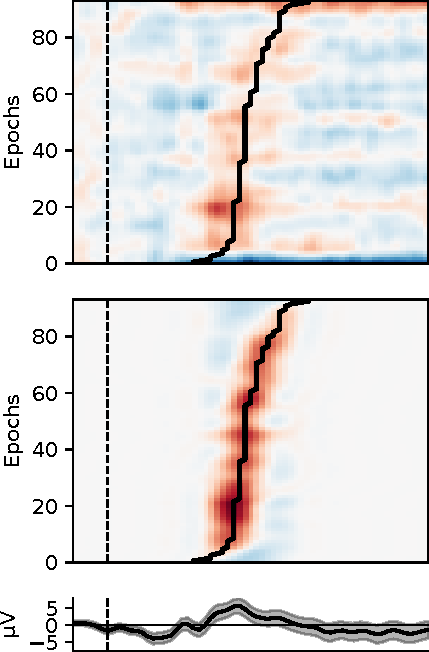
\includegraphics[height=1.3\textwidth]{figures/covert/split_p3_latency_subject.pdf}
  \end{minipage}
  \begin{minipage}{.3\textwidth}
    \emph{After} alignment
    \smallskip

    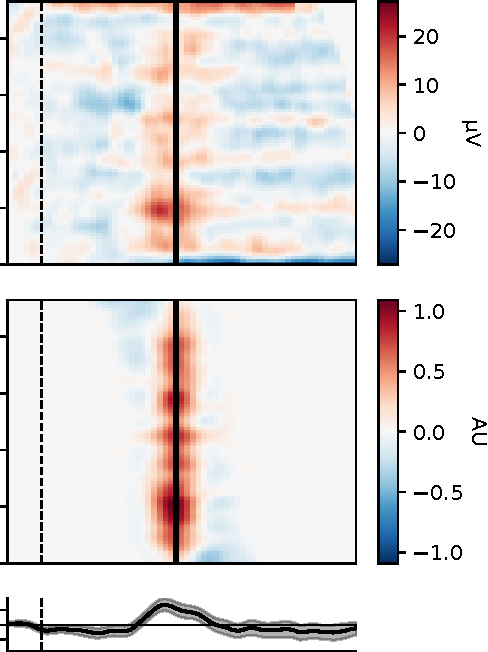
\includegraphics[height=1.3\textwidth]{figures/covert/split_p3_latency_subject_aligned.pdf}
  \end{minipage}
  \aside{
    Developed iterative method based on CBLE
    \bigskip

    Enhances latency estimagion and SNR in simulated data
    \bigskip

    Does this transfer to real data?
  }
\end{frame}


\begin{frame}
  \frametitle{Application to gaze-independent decoding}
  \begin{minipage}{.6\textwidth}
    \centering
    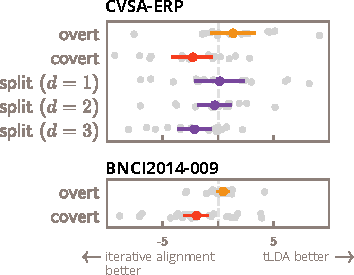
\includegraphics[width=\textwidth]{figures/covert/roc_auc_diff.pdf}
  \end{minipage}\hfill
  \aside{%
    Iterative CBLE can function with unseen data and is applicable as decoder
    \bigskip

    Within-subject, cross-validated single-trial ROC-AUC (\%)
    \bigskip

    Within and across VSA conditions to establish independence
    \bigskip

    Improves decoding performance in gaze-independent settings


  }
\end{frame}
\note{Across: transfer}

% =============================================================================

\outline{\emph{C4:} Evaluation in end-users}{figures/outline_patient.pdf}
\note{
  Now proposed a way to enhance gaze-independent decoding as a proposed
  solution for individuals with eye motor impairment
}

\begin{frame}
  \frametitle{Subjects with physical, speech and gaze impairment}

  \begin{minipage}[c]{.9\textwidth}
  \begin{tabular}{@{}l|lrlrl@{}}
      \textbf{ID}  & \textbf{Diagnosis} & \textbf{Age} &
      \textbf{Speech} & \textbf{Trach.} & \textbf{Communication} \\ \hline
      PA1 & bulbar-onset ALS & 58  & absent  & no          & tablet                 \\
      PB1 & Friedreich's ataxia & 41  & impaired & no          & verbal                 \\
      PB2 & Friedreich's ataxia & 43  & impaired & no          & verbal                 \\
      PB4 & Friedreich's ataxia & 48  & impaired & no          & verbal                 \\
      PC2 & brainstem stroke & 43  & absent  & yes         &  eye movement \\
      PC3 & brainstem stroke & 43  & absent  & yes         & letterboard            \\
      PC4 & cerebellar stroke & 54  & absent  & yes         & letterboard \\
  \end{tabular}
  \end{minipage}\hfill%
  \begin{minipage}[c]{.1\textwidth}
    \centering
    
\includegraphics[width=\textwidth]{figures/logos/uz_leuven.jpg}
    \smallskip

    
\includegraphics[width=.8\textwidth]{figures/logos/chu_lille.png}
    \smallskip

    
\includegraphics[width=\textwidth]{figures/logos/trainm.png}
    \smallskip

    
\includegraphics[width=\textwidth]{figures/logos/fondation-partage-vie.png}
    \smallskip

  \end{minipage}

\end{frame}



\begin{frame}
  \frametitle{Eye motor impairment}
  \newcommand{\skill}{}
  \newcommand{\noskill}{x}
  \newcommand{\snoskill}{o}

  \begin{tabular}{l|ccccccc}
                            & PA1      & PB1      & PB2       & PB4      & PC2       & PC3       & PC4 \\ \hline
    \small Visual fixation         & \noskill & \noskill & \noskill  & \noskill & \noskill  & \noskill  & \noskill \\
    \small Eyelid function         & \skill   & \skill   & \skill    & \skill   &  \skill  & \noskill  & \noskill \\
    \small Ocular motility         & \skill   & \noskill & \skill    & \noskill & \snoskill & \snoskill & \noskill\\
    \small Binocular vision        & \skill   & \skill   & \skill    & \skill   & \noskill  & \snoskill & \snoskill \\
    \small Field of vision         & \skill   & \skill   & \skill    & \skill   & \skill    & \noskill  & \noskill \\
    \small Involuntary movement    & \skill   & \noskill & \snoskill  & \noskill &  \noskill  & \noskill  & \skill \\
  \end{tabular}
  \bigskip

  x: impaired, o: severely impaired
\end{frame}

\begin{frame}
  \frametitle{Off-line covert vsa experiment}

  \begin{minipage}{.6\textwidth}
    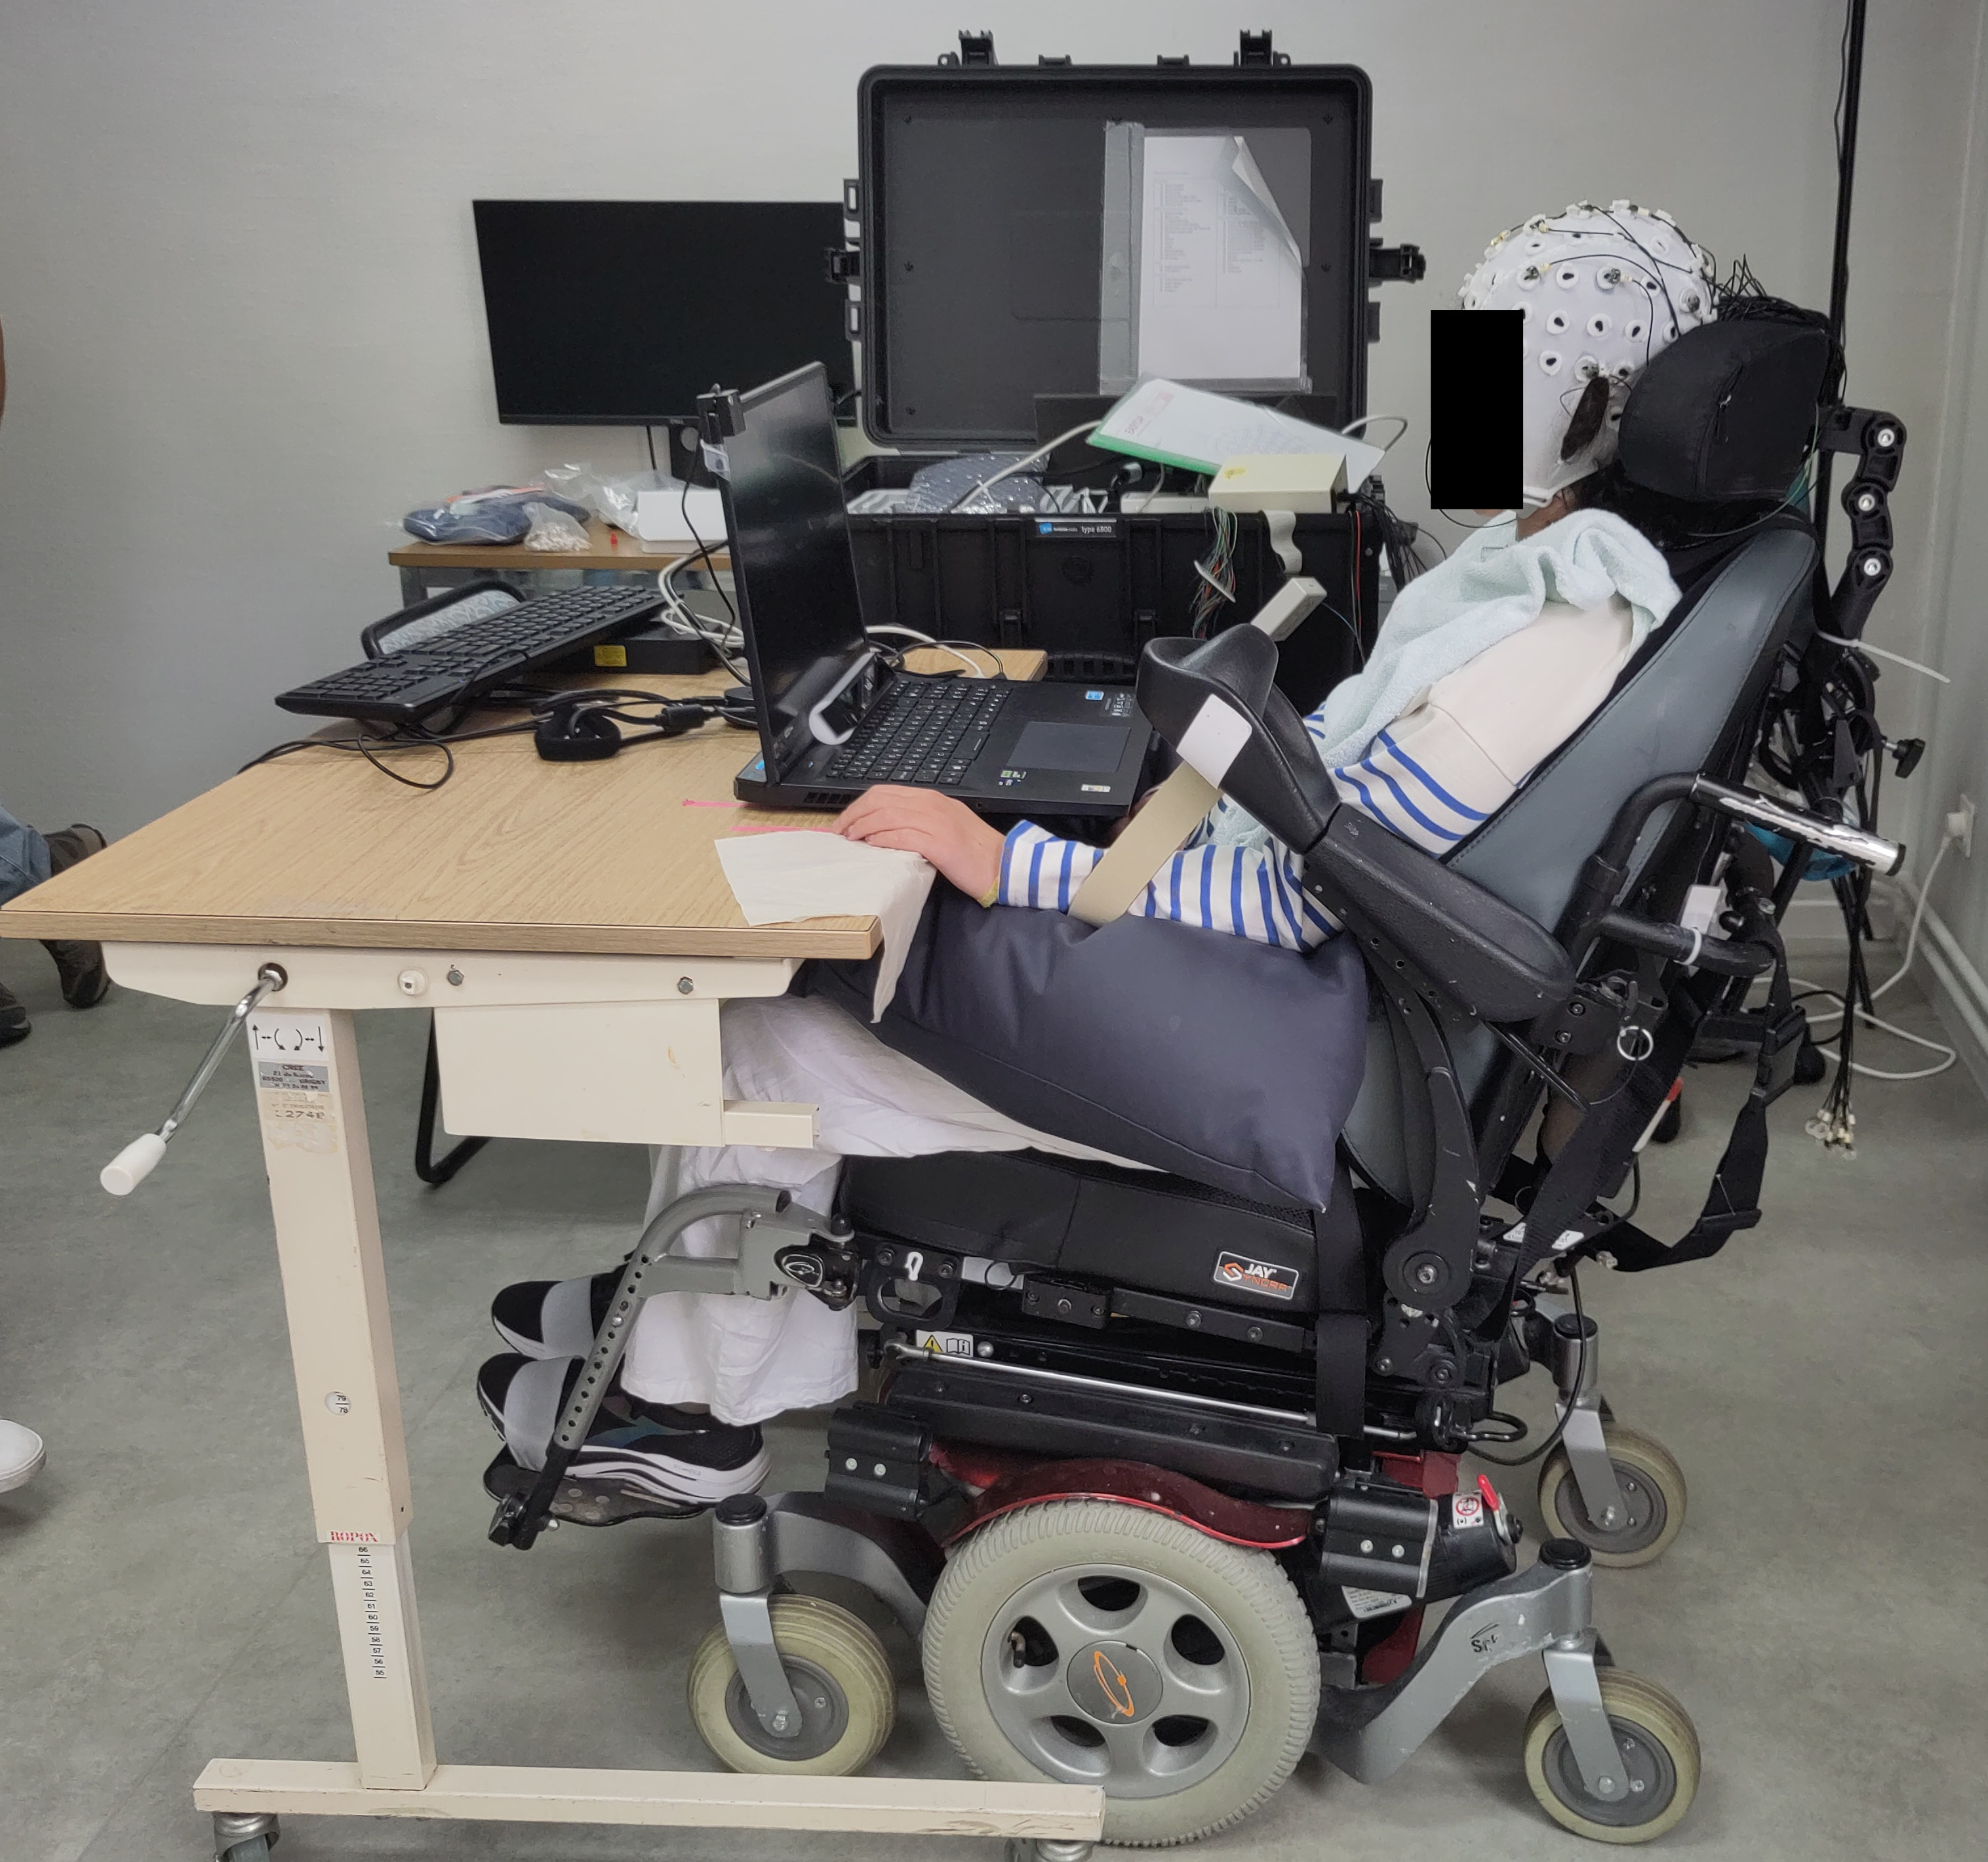
\includegraphics[height=.45\textwidth]{figures/patients/PD01a-obfuscated.jpg}%
    \hfill%
    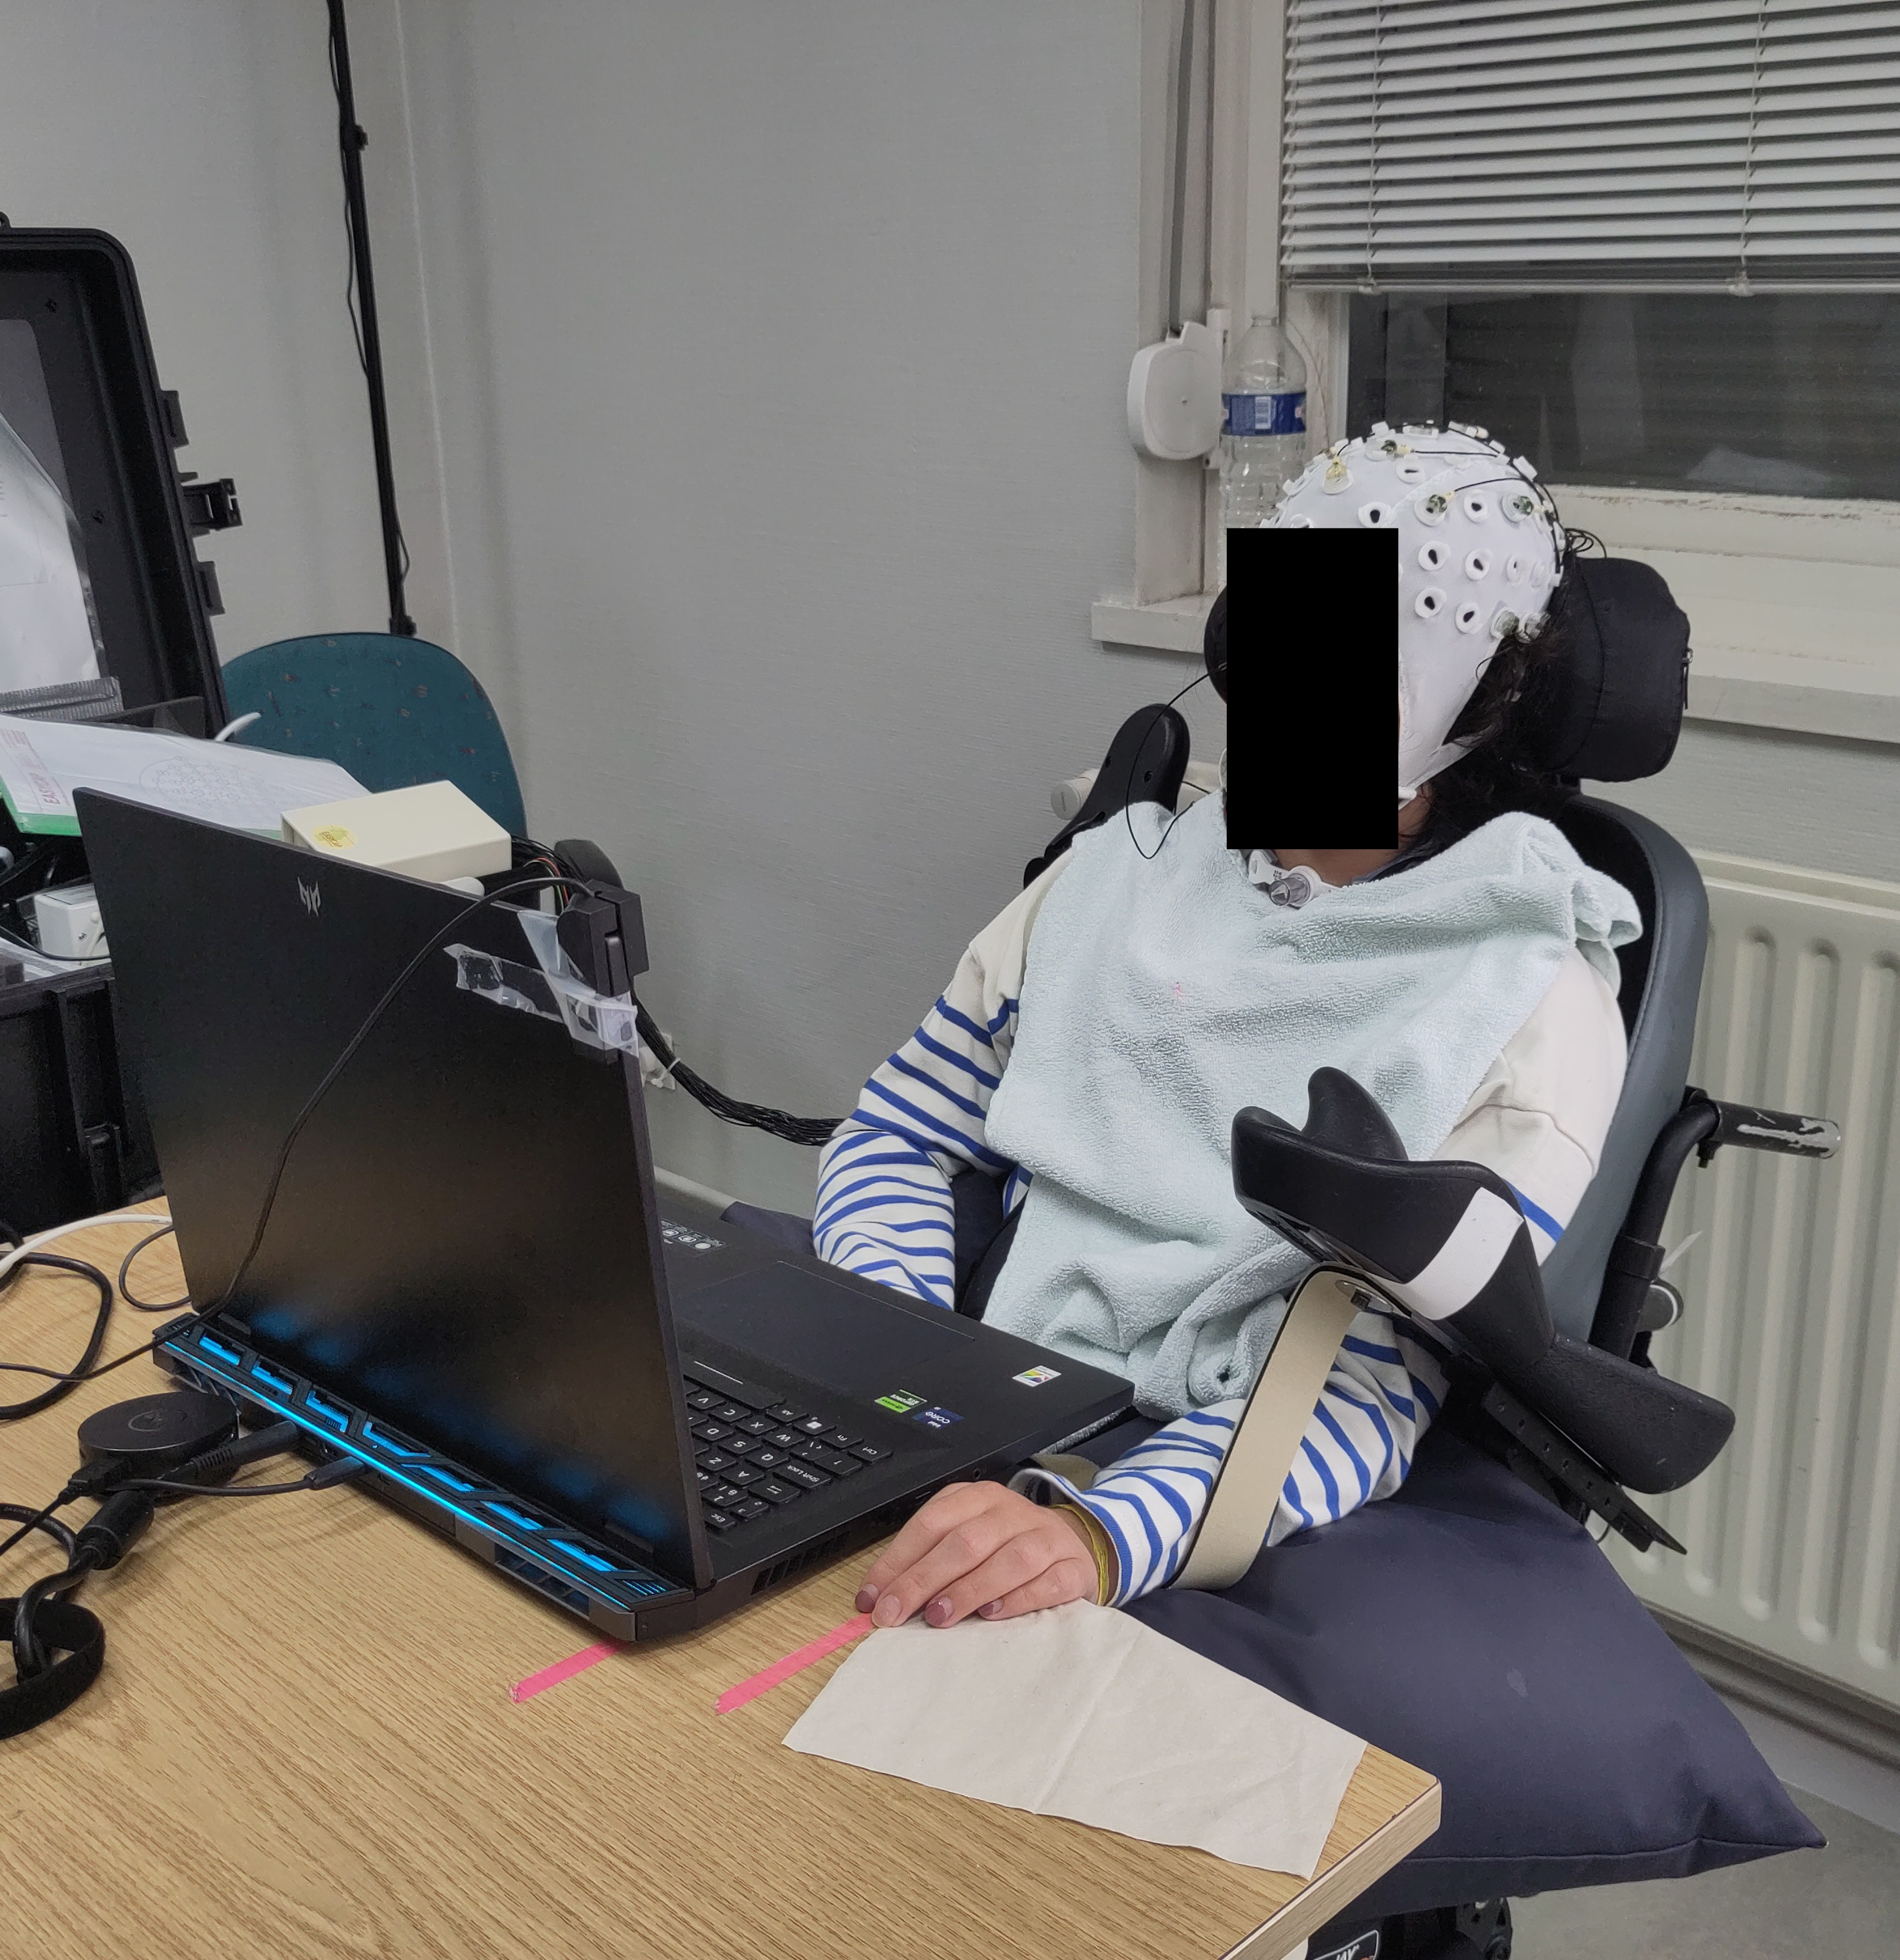
\includegraphics[height=.45\textwidth]{figures/patients/PD01b-obfuscated.jpg}%
    \bigskip

    {\small
    \begin{minipage}{.3\textwidth}
      Overt VSA
      \smallskip

      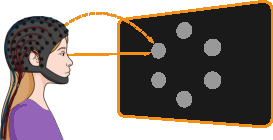
\includegraphics[width=\textwidth]{figures/covert/attention_overt.pdf}
    \end{minipage}\hfill%
    \begin{minipage}{.3\textwidth}
      Covert VSA
      \smallskip

      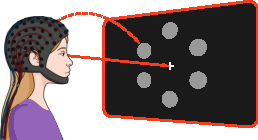
\includegraphics[width=\textwidth]{figures/covert/attention_covert.pdf}
    \end{minipage}\hfill%
    \begin{minipage}{.3\textwidth}
      \small
      Free VSA
      \smallskip

      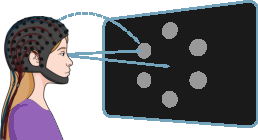
\includegraphics[width=\textwidth]{figures/covert/attention_free.pdf}
    \end{minipage}%
  }
  \end{minipage}


  \aside{
    EEG, EOG and eye-tracking
    \bigskip

    Adapted stimulation parameters
    \bigskip

    Few studies investigating VSA abilities of end-users
    \bigskip

    Replace \textit{split} by \textit{free} to study comfort

  }

\end{frame}

\begin{frame}[c]
  \frametitle{Eye tracking}
  \begin{minipage}{.6\textwidth}
    \centering
    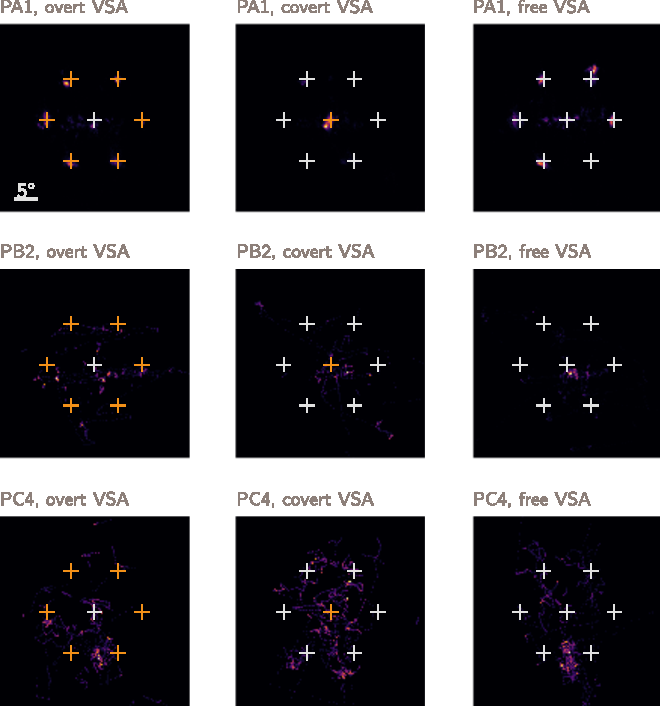
\includegraphics[width=.8\textwidth]{figures/patients/fig_gaze.pdf}
  \end{minipage}
  \aside{
    Most prefered to perform overt VSA
    \bigskip

    Voluntary covert and split VSA did occur
    \bigskip

    Portable eye tracker not always suited

  }
\end{frame}

\begin{frame}
  \frametitle{Subject decoding performance}
  \begin{minipage}{.6\textwidth}
    \resizebox{\textwidth}{!}{
      \hspace{-0.41662707185564984in}
%%% Creator: Matplotlib, PGF backend
%%
%% To include the figure in your LaTeX document, write
%%   \input{<filename>.pgf}
%%
%% Make sure the required packages are loaded in your preamble
%%   \usepackage{pgf}
%%
%% Also ensure that all the required font packages are loaded; for instance,
%% the lmodern package is sometimes necessary when using math font.
%%   \usepackage{lmodern}
%%
%% Figures using additional raster images can only be included by \input if
%% they are in the same directory as the main LaTeX file. For loading figures
%% from other directories you can use the `import` package
%%   \usepackage{import}
%%
%% and then include the figures with
%%   \import{<path to file>}{<filename>.pgf}
%%
%% Matplotlib used the following preamble
%%   \def\mathdefault#1{#1}
%%   \everymath=\expandafter{\the\everymath\displaystyle}
%%   
%%   \ifdefined\pdftexversion\else  % non-pdftex case.
%%     \usepackage{fontspec}
%%   \fi
%%   \makeatletter\@ifpackageloaded{underscore}{}{\usepackage[strings]{underscore}}\makeatother
%%
\begingroup%
\makeatletter%
\begin{pgfpicture}%
\pgfpathrectangle{\pgfpointorigin}{\pgfqpoint{5.057697in}{1.916660in}}%
\pgfusepath{use as bounding box, clip}%
\begin{pgfscope}%
\pgfsetbuttcap%
\pgfsetmiterjoin%
\pgfsetlinewidth{0.000000pt}%
\definecolor{currentstroke}{rgb}{1.000000,1.000000,1.000000}%
\pgfsetstrokecolor{currentstroke}%
\pgfsetstrokeopacity{0.000000}%
\pgfsetdash{}{0pt}%
\pgfpathmoveto{\pgfqpoint{0.000000in}{0.000000in}}%
\pgfpathlineto{\pgfqpoint{5.057697in}{0.000000in}}%
\pgfpathlineto{\pgfqpoint{5.057697in}{1.916660in}}%
\pgfpathlineto{\pgfqpoint{0.000000in}{1.916660in}}%
\pgfpathlineto{\pgfqpoint{0.000000in}{0.000000in}}%
\pgfpathclose%
\pgfusepath{}%
\end{pgfscope}%
\begin{pgfscope}%
\pgfsetbuttcap%
\pgfsetmiterjoin%
\definecolor{currentfill}{rgb}{1.000000,1.000000,1.000000}%
\pgfsetfillcolor{currentfill}%
\pgfsetlinewidth{0.000000pt}%
\definecolor{currentstroke}{rgb}{0.000000,0.000000,0.000000}%
\pgfsetstrokecolor{currentstroke}%
\pgfsetstrokeopacity{0.000000}%
\pgfsetdash{}{0pt}%
\pgfpathmoveto{\pgfqpoint{0.421874in}{0.447433in}}%
\pgfpathlineto{\pgfqpoint{1.911588in}{0.447433in}}%
\pgfpathlineto{\pgfqpoint{1.911588in}{1.746521in}}%
\pgfpathlineto{\pgfqpoint{0.421874in}{1.746521in}}%
\pgfpathlineto{\pgfqpoint{0.421874in}{0.447433in}}%
\pgfpathclose%
\pgfusepath{fill}%
\end{pgfscope}%
\begin{pgfscope}%
\pgfpathrectangle{\pgfqpoint{0.421874in}{0.447433in}}{\pgfqpoint{1.489714in}{1.299088in}}%
\pgfusepath{clip}%
\pgfsetbuttcap%
\pgfsetmiterjoin%
\definecolor{currentfill}{rgb}{0.842157,0.553922,0.200980}%
\pgfsetfillcolor{currentfill}%
\pgfsetlinewidth{0.000000pt}%
\definecolor{currentstroke}{rgb}{0.000000,0.000000,0.000000}%
\pgfsetstrokecolor{currentstroke}%
\pgfsetstrokeopacity{0.000000}%
\pgfsetdash{}{0pt}%
\pgfpathmoveto{\pgfqpoint{0.440495in}{0.447433in}}%
\pgfpathlineto{\pgfqpoint{0.490152in}{0.447433in}}%
\pgfpathlineto{\pgfqpoint{0.490152in}{1.318527in}}%
\pgfpathlineto{\pgfqpoint{0.440495in}{1.318527in}}%
\pgfpathlineto{\pgfqpoint{0.440495in}{0.447433in}}%
\pgfpathclose%
\pgfusepath{fill}%
\end{pgfscope}%
\begin{pgfscope}%
\pgfpathrectangle{\pgfqpoint{0.421874in}{0.447433in}}{\pgfqpoint{1.489714in}{1.299088in}}%
\pgfusepath{clip}%
\pgfsetbuttcap%
\pgfsetmiterjoin%
\definecolor{currentfill}{rgb}{0.842157,0.553922,0.200980}%
\pgfsetfillcolor{currentfill}%
\pgfsetlinewidth{0.000000pt}%
\definecolor{currentstroke}{rgb}{0.000000,0.000000,0.000000}%
\pgfsetstrokecolor{currentstroke}%
\pgfsetstrokeopacity{0.000000}%
\pgfsetdash{}{0pt}%
\pgfpathmoveto{\pgfqpoint{0.626709in}{0.447433in}}%
\pgfpathlineto{\pgfqpoint{0.676367in}{0.447433in}}%
\pgfpathlineto{\pgfqpoint{0.676367in}{1.627122in}}%
\pgfpathlineto{\pgfqpoint{0.626709in}{1.627122in}}%
\pgfpathlineto{\pgfqpoint{0.626709in}{0.447433in}}%
\pgfpathclose%
\pgfusepath{fill}%
\end{pgfscope}%
\begin{pgfscope}%
\pgfpathrectangle{\pgfqpoint{0.421874in}{0.447433in}}{\pgfqpoint{1.489714in}{1.299088in}}%
\pgfusepath{clip}%
\pgfsetbuttcap%
\pgfsetmiterjoin%
\definecolor{currentfill}{rgb}{0.842157,0.553922,0.200980}%
\pgfsetfillcolor{currentfill}%
\pgfsetlinewidth{0.000000pt}%
\definecolor{currentstroke}{rgb}{0.000000,0.000000,0.000000}%
\pgfsetstrokecolor{currentstroke}%
\pgfsetstrokeopacity{0.000000}%
\pgfsetdash{}{0pt}%
\pgfpathmoveto{\pgfqpoint{0.812924in}{0.447433in}}%
\pgfpathlineto{\pgfqpoint{0.862581in}{0.447433in}}%
\pgfpathlineto{\pgfqpoint{0.862581in}{1.528425in}}%
\pgfpathlineto{\pgfqpoint{0.812924in}{1.528425in}}%
\pgfpathlineto{\pgfqpoint{0.812924in}{0.447433in}}%
\pgfpathclose%
\pgfusepath{fill}%
\end{pgfscope}%
\begin{pgfscope}%
\pgfpathrectangle{\pgfqpoint{0.421874in}{0.447433in}}{\pgfqpoint{1.489714in}{1.299088in}}%
\pgfusepath{clip}%
\pgfsetbuttcap%
\pgfsetmiterjoin%
\definecolor{currentfill}{rgb}{0.842157,0.553922,0.200980}%
\pgfsetfillcolor{currentfill}%
\pgfsetlinewidth{0.000000pt}%
\definecolor{currentstroke}{rgb}{0.000000,0.000000,0.000000}%
\pgfsetstrokecolor{currentstroke}%
\pgfsetstrokeopacity{0.000000}%
\pgfsetdash{}{0pt}%
\pgfpathmoveto{\pgfqpoint{0.999138in}{0.447433in}}%
\pgfpathlineto{\pgfqpoint{1.048795in}{0.447433in}}%
\pgfpathlineto{\pgfqpoint{1.048795in}{1.528136in}}%
\pgfpathlineto{\pgfqpoint{0.999138in}{1.528136in}}%
\pgfpathlineto{\pgfqpoint{0.999138in}{0.447433in}}%
\pgfpathclose%
\pgfusepath{fill}%
\end{pgfscope}%
\begin{pgfscope}%
\pgfpathrectangle{\pgfqpoint{0.421874in}{0.447433in}}{\pgfqpoint{1.489714in}{1.299088in}}%
\pgfusepath{clip}%
\pgfsetbuttcap%
\pgfsetmiterjoin%
\definecolor{currentfill}{rgb}{0.842157,0.553922,0.200980}%
\pgfsetfillcolor{currentfill}%
\pgfsetlinewidth{0.000000pt}%
\definecolor{currentstroke}{rgb}{0.000000,0.000000,0.000000}%
\pgfsetstrokecolor{currentstroke}%
\pgfsetstrokeopacity{0.000000}%
\pgfsetdash{}{0pt}%
\pgfpathmoveto{\pgfqpoint{1.185352in}{0.447433in}}%
\pgfpathlineto{\pgfqpoint{1.235009in}{0.447433in}}%
\pgfpathlineto{\pgfqpoint{1.235009in}{1.370255in}}%
\pgfpathlineto{\pgfqpoint{1.185352in}{1.370255in}}%
\pgfpathlineto{\pgfqpoint{1.185352in}{0.447433in}}%
\pgfpathclose%
\pgfusepath{fill}%
\end{pgfscope}%
\begin{pgfscope}%
\pgfpathrectangle{\pgfqpoint{0.421874in}{0.447433in}}{\pgfqpoint{1.489714in}{1.299088in}}%
\pgfusepath{clip}%
\pgfsetbuttcap%
\pgfsetmiterjoin%
\definecolor{currentfill}{rgb}{0.842157,0.553922,0.200980}%
\pgfsetfillcolor{currentfill}%
\pgfsetlinewidth{0.000000pt}%
\definecolor{currentstroke}{rgb}{0.000000,0.000000,0.000000}%
\pgfsetstrokecolor{currentstroke}%
\pgfsetstrokeopacity{0.000000}%
\pgfsetdash{}{0pt}%
\pgfpathmoveto{\pgfqpoint{1.371567in}{0.447433in}}%
\pgfpathlineto{\pgfqpoint{1.421224in}{0.447433in}}%
\pgfpathlineto{\pgfqpoint{1.421224in}{1.363222in}}%
\pgfpathlineto{\pgfqpoint{1.371567in}{1.363222in}}%
\pgfpathlineto{\pgfqpoint{1.371567in}{0.447433in}}%
\pgfpathclose%
\pgfusepath{fill}%
\end{pgfscope}%
\begin{pgfscope}%
\pgfpathrectangle{\pgfqpoint{0.421874in}{0.447433in}}{\pgfqpoint{1.489714in}{1.299088in}}%
\pgfusepath{clip}%
\pgfsetbuttcap%
\pgfsetmiterjoin%
\definecolor{currentfill}{rgb}{0.842157,0.553922,0.200980}%
\pgfsetfillcolor{currentfill}%
\pgfsetlinewidth{0.000000pt}%
\definecolor{currentstroke}{rgb}{0.000000,0.000000,0.000000}%
\pgfsetstrokecolor{currentstroke}%
\pgfsetstrokeopacity{0.000000}%
\pgfsetdash{}{0pt}%
\pgfpathmoveto{\pgfqpoint{1.557781in}{0.447433in}}%
\pgfpathlineto{\pgfqpoint{1.607438in}{0.447433in}}%
\pgfpathlineto{\pgfqpoint{1.607438in}{1.306366in}}%
\pgfpathlineto{\pgfqpoint{1.557781in}{1.306366in}}%
\pgfpathlineto{\pgfqpoint{1.557781in}{0.447433in}}%
\pgfpathclose%
\pgfusepath{fill}%
\end{pgfscope}%
\begin{pgfscope}%
\pgfpathrectangle{\pgfqpoint{0.421874in}{0.447433in}}{\pgfqpoint{1.489714in}{1.299088in}}%
\pgfusepath{clip}%
\pgfsetbuttcap%
\pgfsetmiterjoin%
\definecolor{currentfill}{rgb}{0.842157,0.553922,0.200980}%
\pgfsetfillcolor{currentfill}%
\pgfsetlinewidth{0.000000pt}%
\definecolor{currentstroke}{rgb}{0.000000,0.000000,0.000000}%
\pgfsetstrokecolor{currentstroke}%
\pgfsetstrokeopacity{0.000000}%
\pgfsetdash{}{0pt}%
\pgfpathmoveto{\pgfqpoint{1.743995in}{0.447433in}}%
\pgfpathlineto{\pgfqpoint{1.793652in}{0.447433in}}%
\pgfpathlineto{\pgfqpoint{1.793652in}{1.434579in}}%
\pgfpathlineto{\pgfqpoint{1.743995in}{1.434579in}}%
\pgfpathlineto{\pgfqpoint{1.743995in}{0.447433in}}%
\pgfpathclose%
\pgfusepath{fill}%
\end{pgfscope}%
\begin{pgfscope}%
\pgfpathrectangle{\pgfqpoint{0.421874in}{0.447433in}}{\pgfqpoint{1.489714in}{1.299088in}}%
\pgfusepath{clip}%
\pgfsetbuttcap%
\pgfsetmiterjoin%
\definecolor{currentfill}{rgb}{0.858824,0.314706,0.223529}%
\pgfsetfillcolor{currentfill}%
\pgfsetlinewidth{0.000000pt}%
\definecolor{currentstroke}{rgb}{0.000000,0.000000,0.000000}%
\pgfsetstrokecolor{currentstroke}%
\pgfsetstrokeopacity{0.000000}%
\pgfsetdash{}{0pt}%
\pgfpathmoveto{\pgfqpoint{0.490152in}{0.447433in}}%
\pgfpathlineto{\pgfqpoint{0.539809in}{0.447433in}}%
\pgfpathlineto{\pgfqpoint{0.539809in}{1.376937in}}%
\pgfpathlineto{\pgfqpoint{0.490152in}{1.376937in}}%
\pgfpathlineto{\pgfqpoint{0.490152in}{0.447433in}}%
\pgfpathclose%
\pgfusepath{fill}%
\end{pgfscope}%
\begin{pgfscope}%
\pgfpathrectangle{\pgfqpoint{0.421874in}{0.447433in}}{\pgfqpoint{1.489714in}{1.299088in}}%
\pgfusepath{clip}%
\pgfsetbuttcap%
\pgfsetmiterjoin%
\definecolor{currentfill}{rgb}{0.858824,0.314706,0.223529}%
\pgfsetfillcolor{currentfill}%
\pgfsetlinewidth{0.000000pt}%
\definecolor{currentstroke}{rgb}{0.000000,0.000000,0.000000}%
\pgfsetstrokecolor{currentstroke}%
\pgfsetstrokeopacity{0.000000}%
\pgfsetdash{}{0pt}%
\pgfpathmoveto{\pgfqpoint{0.676367in}{0.447433in}}%
\pgfpathlineto{\pgfqpoint{0.726024in}{0.447433in}}%
\pgfpathlineto{\pgfqpoint{0.726024in}{1.609971in}}%
\pgfpathlineto{\pgfqpoint{0.676367in}{1.609971in}}%
\pgfpathlineto{\pgfqpoint{0.676367in}{0.447433in}}%
\pgfpathclose%
\pgfusepath{fill}%
\end{pgfscope}%
\begin{pgfscope}%
\pgfpathrectangle{\pgfqpoint{0.421874in}{0.447433in}}{\pgfqpoint{1.489714in}{1.299088in}}%
\pgfusepath{clip}%
\pgfsetbuttcap%
\pgfsetmiterjoin%
\definecolor{currentfill}{rgb}{0.858824,0.314706,0.223529}%
\pgfsetfillcolor{currentfill}%
\pgfsetlinewidth{0.000000pt}%
\definecolor{currentstroke}{rgb}{0.000000,0.000000,0.000000}%
\pgfsetstrokecolor{currentstroke}%
\pgfsetstrokeopacity{0.000000}%
\pgfsetdash{}{0pt}%
\pgfpathmoveto{\pgfqpoint{0.862581in}{0.447433in}}%
\pgfpathlineto{\pgfqpoint{0.912238in}{0.447433in}}%
\pgfpathlineto{\pgfqpoint{0.912238in}{1.522529in}}%
\pgfpathlineto{\pgfqpoint{0.862581in}{1.522529in}}%
\pgfpathlineto{\pgfqpoint{0.862581in}{0.447433in}}%
\pgfpathclose%
\pgfusepath{fill}%
\end{pgfscope}%
\begin{pgfscope}%
\pgfpathrectangle{\pgfqpoint{0.421874in}{0.447433in}}{\pgfqpoint{1.489714in}{1.299088in}}%
\pgfusepath{clip}%
\pgfsetbuttcap%
\pgfsetmiterjoin%
\definecolor{currentfill}{rgb}{0.858824,0.314706,0.223529}%
\pgfsetfillcolor{currentfill}%
\pgfsetlinewidth{0.000000pt}%
\definecolor{currentstroke}{rgb}{0.000000,0.000000,0.000000}%
\pgfsetstrokecolor{currentstroke}%
\pgfsetstrokeopacity{0.000000}%
\pgfsetdash{}{0pt}%
\pgfpathmoveto{\pgfqpoint{1.048795in}{0.447433in}}%
\pgfpathlineto{\pgfqpoint{1.098452in}{0.447433in}}%
\pgfpathlineto{\pgfqpoint{1.098452in}{1.493636in}}%
\pgfpathlineto{\pgfqpoint{1.048795in}{1.493636in}}%
\pgfpathlineto{\pgfqpoint{1.048795in}{0.447433in}}%
\pgfpathclose%
\pgfusepath{fill}%
\end{pgfscope}%
\begin{pgfscope}%
\pgfpathrectangle{\pgfqpoint{0.421874in}{0.447433in}}{\pgfqpoint{1.489714in}{1.299088in}}%
\pgfusepath{clip}%
\pgfsetbuttcap%
\pgfsetmiterjoin%
\definecolor{currentfill}{rgb}{0.858824,0.314706,0.223529}%
\pgfsetfillcolor{currentfill}%
\pgfsetlinewidth{0.000000pt}%
\definecolor{currentstroke}{rgb}{0.000000,0.000000,0.000000}%
\pgfsetstrokecolor{currentstroke}%
\pgfsetstrokeopacity{0.000000}%
\pgfsetdash{}{0pt}%
\pgfpathmoveto{\pgfqpoint{1.235009in}{0.447433in}}%
\pgfpathlineto{\pgfqpoint{1.284667in}{0.447433in}}%
\pgfpathlineto{\pgfqpoint{1.284667in}{1.340816in}}%
\pgfpathlineto{\pgfqpoint{1.235009in}{1.340816in}}%
\pgfpathlineto{\pgfqpoint{1.235009in}{0.447433in}}%
\pgfpathclose%
\pgfusepath{fill}%
\end{pgfscope}%
\begin{pgfscope}%
\pgfpathrectangle{\pgfqpoint{0.421874in}{0.447433in}}{\pgfqpoint{1.489714in}{1.299088in}}%
\pgfusepath{clip}%
\pgfsetbuttcap%
\pgfsetmiterjoin%
\definecolor{currentfill}{rgb}{0.858824,0.314706,0.223529}%
\pgfsetfillcolor{currentfill}%
\pgfsetlinewidth{0.000000pt}%
\definecolor{currentstroke}{rgb}{0.000000,0.000000,0.000000}%
\pgfsetstrokecolor{currentstroke}%
\pgfsetstrokeopacity{0.000000}%
\pgfsetdash{}{0pt}%
\pgfpathmoveto{\pgfqpoint{1.421224in}{0.447433in}}%
\pgfpathlineto{\pgfqpoint{1.470881in}{0.447433in}}%
\pgfpathlineto{\pgfqpoint{1.470881in}{1.360833in}}%
\pgfpathlineto{\pgfqpoint{1.421224in}{1.360833in}}%
\pgfpathlineto{\pgfqpoint{1.421224in}{0.447433in}}%
\pgfpathclose%
\pgfusepath{fill}%
\end{pgfscope}%
\begin{pgfscope}%
\pgfpathrectangle{\pgfqpoint{0.421874in}{0.447433in}}{\pgfqpoint{1.489714in}{1.299088in}}%
\pgfusepath{clip}%
\pgfsetbuttcap%
\pgfsetmiterjoin%
\definecolor{currentfill}{rgb}{0.858824,0.314706,0.223529}%
\pgfsetfillcolor{currentfill}%
\pgfsetlinewidth{0.000000pt}%
\definecolor{currentstroke}{rgb}{0.000000,0.000000,0.000000}%
\pgfsetstrokecolor{currentstroke}%
\pgfsetstrokeopacity{0.000000}%
\pgfsetdash{}{0pt}%
\pgfpathmoveto{\pgfqpoint{1.607438in}{0.447433in}}%
\pgfpathlineto{\pgfqpoint{1.657095in}{0.447433in}}%
\pgfpathlineto{\pgfqpoint{1.657095in}{1.300286in}}%
\pgfpathlineto{\pgfqpoint{1.607438in}{1.300286in}}%
\pgfpathlineto{\pgfqpoint{1.607438in}{0.447433in}}%
\pgfpathclose%
\pgfusepath{fill}%
\end{pgfscope}%
\begin{pgfscope}%
\pgfpathrectangle{\pgfqpoint{0.421874in}{0.447433in}}{\pgfqpoint{1.489714in}{1.299088in}}%
\pgfusepath{clip}%
\pgfsetbuttcap%
\pgfsetmiterjoin%
\definecolor{currentfill}{rgb}{0.858824,0.314706,0.223529}%
\pgfsetfillcolor{currentfill}%
\pgfsetlinewidth{0.000000pt}%
\definecolor{currentstroke}{rgb}{0.000000,0.000000,0.000000}%
\pgfsetstrokecolor{currentstroke}%
\pgfsetstrokeopacity{0.000000}%
\pgfsetdash{}{0pt}%
\pgfpathmoveto{\pgfqpoint{1.793652in}{0.447433in}}%
\pgfpathlineto{\pgfqpoint{1.843309in}{0.447433in}}%
\pgfpathlineto{\pgfqpoint{1.843309in}{1.429287in}}%
\pgfpathlineto{\pgfqpoint{1.793652in}{1.429287in}}%
\pgfpathlineto{\pgfqpoint{1.793652in}{0.447433in}}%
\pgfpathclose%
\pgfusepath{fill}%
\end{pgfscope}%
\begin{pgfscope}%
\pgfpathrectangle{\pgfqpoint{0.421874in}{0.447433in}}{\pgfqpoint{1.489714in}{1.299088in}}%
\pgfusepath{clip}%
\pgfsetbuttcap%
\pgfsetmiterjoin%
\definecolor{currentfill}{rgb}{0.464706,0.320588,0.573529}%
\pgfsetfillcolor{currentfill}%
\pgfsetlinewidth{0.000000pt}%
\definecolor{currentstroke}{rgb}{0.000000,0.000000,0.000000}%
\pgfsetstrokecolor{currentstroke}%
\pgfsetstrokeopacity{0.000000}%
\pgfsetdash{}{0pt}%
\pgfpathmoveto{\pgfqpoint{0.539809in}{0.447433in}}%
\pgfpathlineto{\pgfqpoint{0.589467in}{0.447433in}}%
\pgfpathlineto{\pgfqpoint{0.589467in}{1.329460in}}%
\pgfpathlineto{\pgfqpoint{0.539809in}{1.329460in}}%
\pgfpathlineto{\pgfqpoint{0.539809in}{0.447433in}}%
\pgfpathclose%
\pgfusepath{fill}%
\end{pgfscope}%
\begin{pgfscope}%
\pgfpathrectangle{\pgfqpoint{0.421874in}{0.447433in}}{\pgfqpoint{1.489714in}{1.299088in}}%
\pgfusepath{clip}%
\pgfsetbuttcap%
\pgfsetmiterjoin%
\definecolor{currentfill}{rgb}{0.464706,0.320588,0.573529}%
\pgfsetfillcolor{currentfill}%
\pgfsetlinewidth{0.000000pt}%
\definecolor{currentstroke}{rgb}{0.000000,0.000000,0.000000}%
\pgfsetstrokecolor{currentstroke}%
\pgfsetstrokeopacity{0.000000}%
\pgfsetdash{}{0pt}%
\pgfpathmoveto{\pgfqpoint{0.726024in}{0.447433in}}%
\pgfpathlineto{\pgfqpoint{0.775681in}{0.447433in}}%
\pgfpathlineto{\pgfqpoint{0.775681in}{1.611034in}}%
\pgfpathlineto{\pgfqpoint{0.726024in}{1.611034in}}%
\pgfpathlineto{\pgfqpoint{0.726024in}{0.447433in}}%
\pgfpathclose%
\pgfusepath{fill}%
\end{pgfscope}%
\begin{pgfscope}%
\pgfpathrectangle{\pgfqpoint{0.421874in}{0.447433in}}{\pgfqpoint{1.489714in}{1.299088in}}%
\pgfusepath{clip}%
\pgfsetbuttcap%
\pgfsetmiterjoin%
\definecolor{currentfill}{rgb}{0.464706,0.320588,0.573529}%
\pgfsetfillcolor{currentfill}%
\pgfsetlinewidth{0.000000pt}%
\definecolor{currentstroke}{rgb}{0.000000,0.000000,0.000000}%
\pgfsetstrokecolor{currentstroke}%
\pgfsetstrokeopacity{0.000000}%
\pgfsetdash{}{0pt}%
\pgfpathmoveto{\pgfqpoint{0.912238in}{0.447433in}}%
\pgfpathlineto{\pgfqpoint{0.961895in}{0.447433in}}%
\pgfpathlineto{\pgfqpoint{0.961895in}{1.496373in}}%
\pgfpathlineto{\pgfqpoint{0.912238in}{1.496373in}}%
\pgfpathlineto{\pgfqpoint{0.912238in}{0.447433in}}%
\pgfpathclose%
\pgfusepath{fill}%
\end{pgfscope}%
\begin{pgfscope}%
\pgfpathrectangle{\pgfqpoint{0.421874in}{0.447433in}}{\pgfqpoint{1.489714in}{1.299088in}}%
\pgfusepath{clip}%
\pgfsetbuttcap%
\pgfsetmiterjoin%
\definecolor{currentfill}{rgb}{0.464706,0.320588,0.573529}%
\pgfsetfillcolor{currentfill}%
\pgfsetlinewidth{0.000000pt}%
\definecolor{currentstroke}{rgb}{0.000000,0.000000,0.000000}%
\pgfsetstrokecolor{currentstroke}%
\pgfsetstrokeopacity{0.000000}%
\pgfsetdash{}{0pt}%
\pgfpathmoveto{\pgfqpoint{1.098452in}{0.447433in}}%
\pgfpathlineto{\pgfqpoint{1.148109in}{0.447433in}}%
\pgfpathlineto{\pgfqpoint{1.148109in}{1.522782in}}%
\pgfpathlineto{\pgfqpoint{1.098452in}{1.522782in}}%
\pgfpathlineto{\pgfqpoint{1.098452in}{0.447433in}}%
\pgfpathclose%
\pgfusepath{fill}%
\end{pgfscope}%
\begin{pgfscope}%
\pgfpathrectangle{\pgfqpoint{0.421874in}{0.447433in}}{\pgfqpoint{1.489714in}{1.299088in}}%
\pgfusepath{clip}%
\pgfsetbuttcap%
\pgfsetmiterjoin%
\definecolor{currentfill}{rgb}{0.464706,0.320588,0.573529}%
\pgfsetfillcolor{currentfill}%
\pgfsetlinewidth{0.000000pt}%
\definecolor{currentstroke}{rgb}{0.000000,0.000000,0.000000}%
\pgfsetstrokecolor{currentstroke}%
\pgfsetstrokeopacity{0.000000}%
\pgfsetdash{}{0pt}%
\pgfpathmoveto{\pgfqpoint{1.284667in}{0.447433in}}%
\pgfpathlineto{\pgfqpoint{1.334324in}{0.447433in}}%
\pgfpathlineto{\pgfqpoint{1.334324in}{1.373421in}}%
\pgfpathlineto{\pgfqpoint{1.284667in}{1.373421in}}%
\pgfpathlineto{\pgfqpoint{1.284667in}{0.447433in}}%
\pgfpathclose%
\pgfusepath{fill}%
\end{pgfscope}%
\begin{pgfscope}%
\pgfpathrectangle{\pgfqpoint{0.421874in}{0.447433in}}{\pgfqpoint{1.489714in}{1.299088in}}%
\pgfusepath{clip}%
\pgfsetbuttcap%
\pgfsetmiterjoin%
\definecolor{currentfill}{rgb}{0.464706,0.320588,0.573529}%
\pgfsetfillcolor{currentfill}%
\pgfsetlinewidth{0.000000pt}%
\definecolor{currentstroke}{rgb}{0.000000,0.000000,0.000000}%
\pgfsetstrokecolor{currentstroke}%
\pgfsetstrokeopacity{0.000000}%
\pgfsetdash{}{0pt}%
\pgfpathmoveto{\pgfqpoint{1.470881in}{0.447433in}}%
\pgfpathlineto{\pgfqpoint{1.520538in}{0.447433in}}%
\pgfpathlineto{\pgfqpoint{1.520538in}{1.296571in}}%
\pgfpathlineto{\pgfqpoint{1.470881in}{1.296571in}}%
\pgfpathlineto{\pgfqpoint{1.470881in}{0.447433in}}%
\pgfpathclose%
\pgfusepath{fill}%
\end{pgfscope}%
\begin{pgfscope}%
\pgfpathrectangle{\pgfqpoint{0.421874in}{0.447433in}}{\pgfqpoint{1.489714in}{1.299088in}}%
\pgfusepath{clip}%
\pgfsetbuttcap%
\pgfsetmiterjoin%
\definecolor{currentfill}{rgb}{0.464706,0.320588,0.573529}%
\pgfsetfillcolor{currentfill}%
\pgfsetlinewidth{0.000000pt}%
\definecolor{currentstroke}{rgb}{0.000000,0.000000,0.000000}%
\pgfsetstrokecolor{currentstroke}%
\pgfsetstrokeopacity{0.000000}%
\pgfsetdash{}{0pt}%
\pgfpathmoveto{\pgfqpoint{1.657095in}{0.447433in}}%
\pgfpathlineto{\pgfqpoint{1.706752in}{0.447433in}}%
\pgfpathlineto{\pgfqpoint{1.706752in}{1.253068in}}%
\pgfpathlineto{\pgfqpoint{1.657095in}{1.253068in}}%
\pgfpathlineto{\pgfqpoint{1.657095in}{0.447433in}}%
\pgfpathclose%
\pgfusepath{fill}%
\end{pgfscope}%
\begin{pgfscope}%
\pgfpathrectangle{\pgfqpoint{0.421874in}{0.447433in}}{\pgfqpoint{1.489714in}{1.299088in}}%
\pgfusepath{clip}%
\pgfsetbuttcap%
\pgfsetmiterjoin%
\definecolor{currentfill}{rgb}{0.464706,0.320588,0.573529}%
\pgfsetfillcolor{currentfill}%
\pgfsetlinewidth{0.000000pt}%
\definecolor{currentstroke}{rgb}{0.000000,0.000000,0.000000}%
\pgfsetstrokecolor{currentstroke}%
\pgfsetstrokeopacity{0.000000}%
\pgfsetdash{}{0pt}%
\pgfpathmoveto{\pgfqpoint{1.843309in}{0.447433in}}%
\pgfpathlineto{\pgfqpoint{1.892967in}{0.447433in}}%
\pgfpathlineto{\pgfqpoint{1.892967in}{1.411816in}}%
\pgfpathlineto{\pgfqpoint{1.843309in}{1.411816in}}%
\pgfpathlineto{\pgfqpoint{1.843309in}{0.447433in}}%
\pgfpathclose%
\pgfusepath{fill}%
\end{pgfscope}%
\begin{pgfscope}%
\pgfsetbuttcap%
\pgfsetroundjoin%
\definecolor{currentfill}{rgb}{0.552941,0.501961,0.478431}%
\pgfsetfillcolor{currentfill}%
\pgfsetlinewidth{0.803000pt}%
\definecolor{currentstroke}{rgb}{0.552941,0.501961,0.478431}%
\pgfsetstrokecolor{currentstroke}%
\pgfsetdash{}{0pt}%
\pgfsys@defobject{currentmarker}{\pgfqpoint{0.000000in}{0.000000in}}{\pgfqpoint{0.000000in}{0.041667in}}{%
\pgfpathmoveto{\pgfqpoint{0.000000in}{0.000000in}}%
\pgfpathlineto{\pgfqpoint{0.000000in}{0.041667in}}%
\pgfusepath{stroke,fill}%
}%
\begin{pgfscope}%
\pgfsys@transformshift{0.514981in}{0.447433in}%
\pgfsys@useobject{currentmarker}{}%
\end{pgfscope}%
\end{pgfscope}%
\begin{pgfscope}%
\definecolor{textcolor}{rgb}{0.552941,0.501961,0.478431}%
\pgfsetstrokecolor{textcolor}%
\pgfsetfillcolor{textcolor}%
\pgftext[x=0.546231in, y=0.177276in, left, base,rotate=90.000000]{\color{textcolor}{\sffamily\fontsize{9.000000}{10.800000}\selectfont\catcode`\^=\active\def^{\ifmmode\sp\else\^{}\fi}\catcode`\%=\active\def%{\%}PA1}}%
\end{pgfscope}%
\begin{pgfscope}%
\pgfsetbuttcap%
\pgfsetroundjoin%
\definecolor{currentfill}{rgb}{0.552941,0.501961,0.478431}%
\pgfsetfillcolor{currentfill}%
\pgfsetlinewidth{0.803000pt}%
\definecolor{currentstroke}{rgb}{0.552941,0.501961,0.478431}%
\pgfsetstrokecolor{currentstroke}%
\pgfsetdash{}{0pt}%
\pgfsys@defobject{currentmarker}{\pgfqpoint{0.000000in}{0.000000in}}{\pgfqpoint{0.000000in}{0.041667in}}{%
\pgfpathmoveto{\pgfqpoint{0.000000in}{0.000000in}}%
\pgfpathlineto{\pgfqpoint{0.000000in}{0.041667in}}%
\pgfusepath{stroke,fill}%
}%
\begin{pgfscope}%
\pgfsys@transformshift{0.701195in}{0.447433in}%
\pgfsys@useobject{currentmarker}{}%
\end{pgfscope}%
\end{pgfscope}%
\begin{pgfscope}%
\definecolor{textcolor}{rgb}{0.552941,0.501961,0.478431}%
\pgfsetstrokecolor{textcolor}%
\pgfsetfillcolor{textcolor}%
\pgftext[x=0.732445in, y=0.166667in, left, base,rotate=90.000000]{\color{textcolor}{\sffamily\fontsize{9.000000}{10.800000}\selectfont\catcode`\^=\active\def^{\ifmmode\sp\else\^{}\fi}\catcode`\%=\active\def%{\%}PB1}}%
\end{pgfscope}%
\begin{pgfscope}%
\pgfsetbuttcap%
\pgfsetroundjoin%
\definecolor{currentfill}{rgb}{0.552941,0.501961,0.478431}%
\pgfsetfillcolor{currentfill}%
\pgfsetlinewidth{0.803000pt}%
\definecolor{currentstroke}{rgb}{0.552941,0.501961,0.478431}%
\pgfsetstrokecolor{currentstroke}%
\pgfsetdash{}{0pt}%
\pgfsys@defobject{currentmarker}{\pgfqpoint{0.000000in}{0.000000in}}{\pgfqpoint{0.000000in}{0.041667in}}{%
\pgfpathmoveto{\pgfqpoint{0.000000in}{0.000000in}}%
\pgfpathlineto{\pgfqpoint{0.000000in}{0.041667in}}%
\pgfusepath{stroke,fill}%
}%
\begin{pgfscope}%
\pgfsys@transformshift{0.887409in}{0.447433in}%
\pgfsys@useobject{currentmarker}{}%
\end{pgfscope}%
\end{pgfscope}%
\begin{pgfscope}%
\definecolor{textcolor}{rgb}{0.552941,0.501961,0.478431}%
\pgfsetstrokecolor{textcolor}%
\pgfsetfillcolor{textcolor}%
\pgftext[x=0.918659in, y=0.166667in, left, base,rotate=90.000000]{\color{textcolor}{\sffamily\fontsize{9.000000}{10.800000}\selectfont\catcode`\^=\active\def^{\ifmmode\sp\else\^{}\fi}\catcode`\%=\active\def%{\%}PB2}}%
\end{pgfscope}%
\begin{pgfscope}%
\pgfsetbuttcap%
\pgfsetroundjoin%
\definecolor{currentfill}{rgb}{0.552941,0.501961,0.478431}%
\pgfsetfillcolor{currentfill}%
\pgfsetlinewidth{0.803000pt}%
\definecolor{currentstroke}{rgb}{0.552941,0.501961,0.478431}%
\pgfsetstrokecolor{currentstroke}%
\pgfsetdash{}{0pt}%
\pgfsys@defobject{currentmarker}{\pgfqpoint{0.000000in}{0.000000in}}{\pgfqpoint{0.000000in}{0.041667in}}{%
\pgfpathmoveto{\pgfqpoint{0.000000in}{0.000000in}}%
\pgfpathlineto{\pgfqpoint{0.000000in}{0.041667in}}%
\pgfusepath{stroke,fill}%
}%
\begin{pgfscope}%
\pgfsys@transformshift{1.073624in}{0.447433in}%
\pgfsys@useobject{currentmarker}{}%
\end{pgfscope}%
\end{pgfscope}%
\begin{pgfscope}%
\definecolor{textcolor}{rgb}{0.552941,0.501961,0.478431}%
\pgfsetstrokecolor{textcolor}%
\pgfsetfillcolor{textcolor}%
\pgftext[x=1.104874in, y=0.166667in, left, base,rotate=90.000000]{\color{textcolor}{\sffamily\fontsize{9.000000}{10.800000}\selectfont\catcode`\^=\active\def^{\ifmmode\sp\else\^{}\fi}\catcode`\%=\active\def%{\%}PB4}}%
\end{pgfscope}%
\begin{pgfscope}%
\pgfsetbuttcap%
\pgfsetroundjoin%
\definecolor{currentfill}{rgb}{0.552941,0.501961,0.478431}%
\pgfsetfillcolor{currentfill}%
\pgfsetlinewidth{0.803000pt}%
\definecolor{currentstroke}{rgb}{0.552941,0.501961,0.478431}%
\pgfsetstrokecolor{currentstroke}%
\pgfsetdash{}{0pt}%
\pgfsys@defobject{currentmarker}{\pgfqpoint{0.000000in}{0.000000in}}{\pgfqpoint{0.000000in}{0.041667in}}{%
\pgfpathmoveto{\pgfqpoint{0.000000in}{0.000000in}}%
\pgfpathlineto{\pgfqpoint{0.000000in}{0.041667in}}%
\pgfusepath{stroke,fill}%
}%
\begin{pgfscope}%
\pgfsys@transformshift{1.259838in}{0.447433in}%
\pgfsys@useobject{currentmarker}{}%
\end{pgfscope}%
\end{pgfscope}%
\begin{pgfscope}%
\definecolor{textcolor}{rgb}{0.552941,0.501961,0.478431}%
\pgfsetstrokecolor{textcolor}%
\pgfsetfillcolor{textcolor}%
\pgftext[x=1.291088in, y=0.170332in, left, base,rotate=90.000000]{\color{textcolor}{\sffamily\fontsize{9.000000}{10.800000}\selectfont\catcode`\^=\active\def^{\ifmmode\sp\else\^{}\fi}\catcode`\%=\active\def%{\%}PC2}}%
\end{pgfscope}%
\begin{pgfscope}%
\pgfsetbuttcap%
\pgfsetroundjoin%
\definecolor{currentfill}{rgb}{0.552941,0.501961,0.478431}%
\pgfsetfillcolor{currentfill}%
\pgfsetlinewidth{0.803000pt}%
\definecolor{currentstroke}{rgb}{0.552941,0.501961,0.478431}%
\pgfsetstrokecolor{currentstroke}%
\pgfsetdash{}{0pt}%
\pgfsys@defobject{currentmarker}{\pgfqpoint{0.000000in}{0.000000in}}{\pgfqpoint{0.000000in}{0.041667in}}{%
\pgfpathmoveto{\pgfqpoint{0.000000in}{0.000000in}}%
\pgfpathlineto{\pgfqpoint{0.000000in}{0.041667in}}%
\pgfusepath{stroke,fill}%
}%
\begin{pgfscope}%
\pgfsys@transformshift{1.446052in}{0.447433in}%
\pgfsys@useobject{currentmarker}{}%
\end{pgfscope}%
\end{pgfscope}%
\begin{pgfscope}%
\definecolor{textcolor}{rgb}{0.552941,0.501961,0.478431}%
\pgfsetstrokecolor{textcolor}%
\pgfsetfillcolor{textcolor}%
\pgftext[x=1.477302in, y=0.170332in, left, base,rotate=90.000000]{\color{textcolor}{\sffamily\fontsize{9.000000}{10.800000}\selectfont\catcode`\^=\active\def^{\ifmmode\sp\else\^{}\fi}\catcode`\%=\active\def%{\%}PC3}}%
\end{pgfscope}%
\begin{pgfscope}%
\pgfsetbuttcap%
\pgfsetroundjoin%
\definecolor{currentfill}{rgb}{0.552941,0.501961,0.478431}%
\pgfsetfillcolor{currentfill}%
\pgfsetlinewidth{0.803000pt}%
\definecolor{currentstroke}{rgb}{0.552941,0.501961,0.478431}%
\pgfsetstrokecolor{currentstroke}%
\pgfsetdash{}{0pt}%
\pgfsys@defobject{currentmarker}{\pgfqpoint{0.000000in}{0.000000in}}{\pgfqpoint{0.000000in}{0.041667in}}{%
\pgfpathmoveto{\pgfqpoint{0.000000in}{0.000000in}}%
\pgfpathlineto{\pgfqpoint{0.000000in}{0.041667in}}%
\pgfusepath{stroke,fill}%
}%
\begin{pgfscope}%
\pgfsys@transformshift{1.632267in}{0.447433in}%
\pgfsys@useobject{currentmarker}{}%
\end{pgfscope}%
\end{pgfscope}%
\begin{pgfscope}%
\definecolor{textcolor}{rgb}{0.552941,0.501961,0.478431}%
\pgfsetstrokecolor{textcolor}%
\pgfsetfillcolor{textcolor}%
\pgftext[x=1.663517in, y=0.170332in, left, base,rotate=90.000000]{\color{textcolor}{\sffamily\fontsize{9.000000}{10.800000}\selectfont\catcode`\^=\active\def^{\ifmmode\sp\else\^{}\fi}\catcode`\%=\active\def%{\%}PC4}}%
\end{pgfscope}%
\begin{pgfscope}%
\pgfsetbuttcap%
\pgfsetroundjoin%
\definecolor{currentfill}{rgb}{0.552941,0.501961,0.478431}%
\pgfsetfillcolor{currentfill}%
\pgfsetlinewidth{0.803000pt}%
\definecolor{currentstroke}{rgb}{0.552941,0.501961,0.478431}%
\pgfsetstrokecolor{currentstroke}%
\pgfsetdash{}{0pt}%
\pgfsys@defobject{currentmarker}{\pgfqpoint{0.000000in}{0.000000in}}{\pgfqpoint{0.000000in}{0.041667in}}{%
\pgfpathmoveto{\pgfqpoint{0.000000in}{0.000000in}}%
\pgfpathlineto{\pgfqpoint{0.000000in}{0.041667in}}%
\pgfusepath{stroke,fill}%
}%
\begin{pgfscope}%
\pgfsys@transformshift{1.818481in}{0.447433in}%
\pgfsys@useobject{currentmarker}{}%
\end{pgfscope}%
\end{pgfscope}%
\begin{pgfscope}%
\definecolor{textcolor}{rgb}{0.552941,0.501961,0.478431}%
\pgfsetstrokecolor{textcolor}%
\pgfsetfillcolor{textcolor}%
\pgftext[x=1.849731in, y=0.177952in, left, base,rotate=90.000000]{\color{textcolor}{\sffamily\fontsize{9.000000}{10.800000}\selectfont\catcode`\^=\active\def^{\ifmmode\sp\else\^{}\fi}\catcode`\%=\active\def%{\%}avg.}}%
\end{pgfscope}%
\begin{pgfscope}%
\definecolor{textcolor}{rgb}{0.552941,0.501961,0.478431}%
\pgfsetstrokecolor{textcolor}%
\pgfsetfillcolor{textcolor}%
\pgftext[x=1.166731in,y=0.111111in,,top]{\color{textcolor}{\sffamily\fontsize{9.000000}{10.800000}\selectfont\catcode`\^=\active\def^{\ifmmode\sp\else\^{}\fi}\catcode`\%=\active\def%{\%}participant}}%
\end{pgfscope}%
\begin{pgfscope}%
\pgfsetbuttcap%
\pgfsetroundjoin%
\definecolor{currentfill}{rgb}{0.552941,0.501961,0.478431}%
\pgfsetfillcolor{currentfill}%
\pgfsetlinewidth{0.803000pt}%
\definecolor{currentstroke}{rgb}{0.552941,0.501961,0.478431}%
\pgfsetstrokecolor{currentstroke}%
\pgfsetdash{}{0pt}%
\pgfsys@defobject{currentmarker}{\pgfqpoint{0.000000in}{0.000000in}}{\pgfqpoint{0.041667in}{0.000000in}}{%
\pgfpathmoveto{\pgfqpoint{0.000000in}{0.000000in}}%
\pgfpathlineto{\pgfqpoint{0.041667in}{0.000000in}}%
\pgfusepath{stroke,fill}%
}%
\begin{pgfscope}%
\pgfsys@transformshift{0.421874in}{0.447433in}%
\pgfsys@useobject{currentmarker}{}%
\end{pgfscope}%
\end{pgfscope}%
\begin{pgfscope}%
\definecolor{textcolor}{rgb}{0.552941,0.501961,0.478431}%
\pgfsetstrokecolor{textcolor}%
\pgfsetfillcolor{textcolor}%
\pgftext[x=0.309027in, y=0.404030in, left, base]{\color{textcolor}{\sffamily\fontsize{9.000000}{10.800000}\selectfont\catcode`\^=\active\def^{\ifmmode\sp\else\^{}\fi}\catcode`\%=\active\def%{\%}0}}%
\end{pgfscope}%
\begin{pgfscope}%
\pgfsetbuttcap%
\pgfsetroundjoin%
\definecolor{currentfill}{rgb}{0.552941,0.501961,0.478431}%
\pgfsetfillcolor{currentfill}%
\pgfsetlinewidth{0.803000pt}%
\definecolor{currentstroke}{rgb}{0.552941,0.501961,0.478431}%
\pgfsetstrokecolor{currentstroke}%
\pgfsetdash{}{0pt}%
\pgfsys@defobject{currentmarker}{\pgfqpoint{0.000000in}{0.000000in}}{\pgfqpoint{0.041667in}{0.000000in}}{%
\pgfpathmoveto{\pgfqpoint{0.000000in}{0.000000in}}%
\pgfpathlineto{\pgfqpoint{0.041667in}{0.000000in}}%
\pgfusepath{stroke,fill}%
}%
\begin{pgfscope}%
\pgfsys@transformshift{0.421874in}{0.707250in}%
\pgfsys@useobject{currentmarker}{}%
\end{pgfscope}%
\end{pgfscope}%
\begin{pgfscope}%
\definecolor{textcolor}{rgb}{0.552941,0.501961,0.478431}%
\pgfsetstrokecolor{textcolor}%
\pgfsetfillcolor{textcolor}%
\pgftext[x=0.244791in, y=0.663848in, left, base]{\color{textcolor}{\sffamily\fontsize{9.000000}{10.800000}\selectfont\catcode`\^=\active\def^{\ifmmode\sp\else\^{}\fi}\catcode`\%=\active\def%{\%}20}}%
\end{pgfscope}%
\begin{pgfscope}%
\pgfsetbuttcap%
\pgfsetroundjoin%
\definecolor{currentfill}{rgb}{0.552941,0.501961,0.478431}%
\pgfsetfillcolor{currentfill}%
\pgfsetlinewidth{0.803000pt}%
\definecolor{currentstroke}{rgb}{0.552941,0.501961,0.478431}%
\pgfsetstrokecolor{currentstroke}%
\pgfsetdash{}{0pt}%
\pgfsys@defobject{currentmarker}{\pgfqpoint{0.000000in}{0.000000in}}{\pgfqpoint{0.041667in}{0.000000in}}{%
\pgfpathmoveto{\pgfqpoint{0.000000in}{0.000000in}}%
\pgfpathlineto{\pgfqpoint{0.041667in}{0.000000in}}%
\pgfusepath{stroke,fill}%
}%
\begin{pgfscope}%
\pgfsys@transformshift{0.421874in}{0.967068in}%
\pgfsys@useobject{currentmarker}{}%
\end{pgfscope}%
\end{pgfscope}%
\begin{pgfscope}%
\definecolor{textcolor}{rgb}{0.552941,0.501961,0.478431}%
\pgfsetstrokecolor{textcolor}%
\pgfsetfillcolor{textcolor}%
\pgftext[x=0.244791in, y=0.923665in, left, base]{\color{textcolor}{\sffamily\fontsize{9.000000}{10.800000}\selectfont\catcode`\^=\active\def^{\ifmmode\sp\else\^{}\fi}\catcode`\%=\active\def%{\%}40}}%
\end{pgfscope}%
\begin{pgfscope}%
\pgfsetbuttcap%
\pgfsetroundjoin%
\definecolor{currentfill}{rgb}{0.552941,0.501961,0.478431}%
\pgfsetfillcolor{currentfill}%
\pgfsetlinewidth{0.803000pt}%
\definecolor{currentstroke}{rgb}{0.552941,0.501961,0.478431}%
\pgfsetstrokecolor{currentstroke}%
\pgfsetdash{}{0pt}%
\pgfsys@defobject{currentmarker}{\pgfqpoint{0.000000in}{0.000000in}}{\pgfqpoint{0.041667in}{0.000000in}}{%
\pgfpathmoveto{\pgfqpoint{0.000000in}{0.000000in}}%
\pgfpathlineto{\pgfqpoint{0.041667in}{0.000000in}}%
\pgfusepath{stroke,fill}%
}%
\begin{pgfscope}%
\pgfsys@transformshift{0.421874in}{1.226886in}%
\pgfsys@useobject{currentmarker}{}%
\end{pgfscope}%
\end{pgfscope}%
\begin{pgfscope}%
\definecolor{textcolor}{rgb}{0.552941,0.501961,0.478431}%
\pgfsetstrokecolor{textcolor}%
\pgfsetfillcolor{textcolor}%
\pgftext[x=0.244791in, y=1.183483in, left, base]{\color{textcolor}{\sffamily\fontsize{9.000000}{10.800000}\selectfont\catcode`\^=\active\def^{\ifmmode\sp\else\^{}\fi}\catcode`\%=\active\def%{\%}60}}%
\end{pgfscope}%
\begin{pgfscope}%
\pgfsetbuttcap%
\pgfsetroundjoin%
\definecolor{currentfill}{rgb}{0.552941,0.501961,0.478431}%
\pgfsetfillcolor{currentfill}%
\pgfsetlinewidth{0.803000pt}%
\definecolor{currentstroke}{rgb}{0.552941,0.501961,0.478431}%
\pgfsetstrokecolor{currentstroke}%
\pgfsetdash{}{0pt}%
\pgfsys@defobject{currentmarker}{\pgfqpoint{0.000000in}{0.000000in}}{\pgfqpoint{0.041667in}{0.000000in}}{%
\pgfpathmoveto{\pgfqpoint{0.000000in}{0.000000in}}%
\pgfpathlineto{\pgfqpoint{0.041667in}{0.000000in}}%
\pgfusepath{stroke,fill}%
}%
\begin{pgfscope}%
\pgfsys@transformshift{0.421874in}{1.486703in}%
\pgfsys@useobject{currentmarker}{}%
\end{pgfscope}%
\end{pgfscope}%
\begin{pgfscope}%
\definecolor{textcolor}{rgb}{0.552941,0.501961,0.478431}%
\pgfsetstrokecolor{textcolor}%
\pgfsetfillcolor{textcolor}%
\pgftext[x=0.244791in, y=1.443301in, left, base]{\color{textcolor}{\sffamily\fontsize{9.000000}{10.800000}\selectfont\catcode`\^=\active\def^{\ifmmode\sp\else\^{}\fi}\catcode`\%=\active\def%{\%}80}}%
\end{pgfscope}%
\begin{pgfscope}%
\pgfsetbuttcap%
\pgfsetroundjoin%
\definecolor{currentfill}{rgb}{0.552941,0.501961,0.478431}%
\pgfsetfillcolor{currentfill}%
\pgfsetlinewidth{0.803000pt}%
\definecolor{currentstroke}{rgb}{0.552941,0.501961,0.478431}%
\pgfsetstrokecolor{currentstroke}%
\pgfsetdash{}{0pt}%
\pgfsys@defobject{currentmarker}{\pgfqpoint{0.000000in}{0.000000in}}{\pgfqpoint{0.041667in}{0.000000in}}{%
\pgfpathmoveto{\pgfqpoint{0.000000in}{0.000000in}}%
\pgfpathlineto{\pgfqpoint{0.041667in}{0.000000in}}%
\pgfusepath{stroke,fill}%
}%
\begin{pgfscope}%
\pgfsys@transformshift{0.421874in}{1.746521in}%
\pgfsys@useobject{currentmarker}{}%
\end{pgfscope}%
\end{pgfscope}%
\begin{pgfscope}%
\definecolor{textcolor}{rgb}{0.552941,0.501961,0.478431}%
\pgfsetstrokecolor{textcolor}%
\pgfsetfillcolor{textcolor}%
\pgftext[x=0.180556in, y=1.703118in, left, base]{\color{textcolor}{\sffamily\fontsize{9.000000}{10.800000}\selectfont\catcode`\^=\active\def^{\ifmmode\sp\else\^{}\fi}\catcode`\%=\active\def%{\%}100}}%
\end{pgfscope}%
\begin{pgfscope}%
\definecolor{textcolor}{rgb}{0.552941,0.501961,0.478431}%
\pgfsetstrokecolor{textcolor}%
\pgfsetfillcolor{textcolor}%
\pgftext[x=0.125000in,y=1.096977in,,bottom,rotate=90.000000]{\color{textcolor}{\sffamily\fontsize{9.000000}{10.800000}\selectfont\catcode`\^=\active\def^{\ifmmode\sp\else\^{}\fi}\catcode`\%=\active\def%{\%}ROC-AUC (\%)}}%
\end{pgfscope}%
\begin{pgfscope}%
\pgfpathrectangle{\pgfqpoint{0.421874in}{0.447433in}}{\pgfqpoint{1.489714in}{1.299088in}}%
\pgfusepath{clip}%
\pgfsetrectcap%
\pgfsetroundjoin%
\pgfsetlinewidth{2.258437pt}%
\definecolor{currentstroke}{rgb}{0.260000,0.260000,0.260000}%
\pgfsetstrokecolor{currentstroke}%
\pgfsetdash{}{0pt}%
\pgfpathmoveto{\pgfqpoint{0.465324in}{1.234568in}}%
\pgfpathlineto{\pgfqpoint{0.465324in}{1.415464in}}%
\pgfusepath{stroke}%
\end{pgfscope}%
\begin{pgfscope}%
\pgfpathrectangle{\pgfqpoint{0.421874in}{0.447433in}}{\pgfqpoint{1.489714in}{1.299088in}}%
\pgfusepath{clip}%
\pgfsetrectcap%
\pgfsetroundjoin%
\pgfsetlinewidth{2.258437pt}%
\definecolor{currentstroke}{rgb}{0.260000,0.260000,0.260000}%
\pgfsetstrokecolor{currentstroke}%
\pgfsetdash{}{0pt}%
\pgfpathmoveto{\pgfqpoint{0.651538in}{1.561052in}}%
\pgfpathlineto{\pgfqpoint{0.651538in}{1.686093in}}%
\pgfusepath{stroke}%
\end{pgfscope}%
\begin{pgfscope}%
\pgfpathrectangle{\pgfqpoint{0.421874in}{0.447433in}}{\pgfqpoint{1.489714in}{1.299088in}}%
\pgfusepath{clip}%
\pgfsetrectcap%
\pgfsetroundjoin%
\pgfsetlinewidth{2.258437pt}%
\definecolor{currentstroke}{rgb}{0.260000,0.260000,0.260000}%
\pgfsetstrokecolor{currentstroke}%
\pgfsetdash{}{0pt}%
\pgfpathmoveto{\pgfqpoint{0.837752in}{1.461055in}}%
\pgfpathlineto{\pgfqpoint{0.837752in}{1.593439in}}%
\pgfusepath{stroke}%
\end{pgfscope}%
\begin{pgfscope}%
\pgfpathrectangle{\pgfqpoint{0.421874in}{0.447433in}}{\pgfqpoint{1.489714in}{1.299088in}}%
\pgfusepath{clip}%
\pgfsetrectcap%
\pgfsetroundjoin%
\pgfsetlinewidth{2.258437pt}%
\definecolor{currentstroke}{rgb}{0.260000,0.260000,0.260000}%
\pgfsetstrokecolor{currentstroke}%
\pgfsetdash{}{0pt}%
\pgfpathmoveto{\pgfqpoint{1.023967in}{1.498414in}}%
\pgfpathlineto{\pgfqpoint{1.023967in}{1.558189in}}%
\pgfusepath{stroke}%
\end{pgfscope}%
\begin{pgfscope}%
\pgfpathrectangle{\pgfqpoint{0.421874in}{0.447433in}}{\pgfqpoint{1.489714in}{1.299088in}}%
\pgfusepath{clip}%
\pgfsetrectcap%
\pgfsetroundjoin%
\pgfsetlinewidth{2.258437pt}%
\definecolor{currentstroke}{rgb}{0.260000,0.260000,0.260000}%
\pgfsetstrokecolor{currentstroke}%
\pgfsetdash{}{0pt}%
\pgfpathmoveto{\pgfqpoint{1.210181in}{1.273321in}}%
\pgfpathlineto{\pgfqpoint{1.210181in}{1.457600in}}%
\pgfusepath{stroke}%
\end{pgfscope}%
\begin{pgfscope}%
\pgfpathrectangle{\pgfqpoint{0.421874in}{0.447433in}}{\pgfqpoint{1.489714in}{1.299088in}}%
\pgfusepath{clip}%
\pgfsetrectcap%
\pgfsetroundjoin%
\pgfsetlinewidth{2.258437pt}%
\definecolor{currentstroke}{rgb}{0.260000,0.260000,0.260000}%
\pgfsetstrokecolor{currentstroke}%
\pgfsetdash{}{0pt}%
\pgfpathmoveto{\pgfqpoint{1.396395in}{1.309172in}}%
\pgfpathlineto{\pgfqpoint{1.396395in}{1.430489in}}%
\pgfusepath{stroke}%
\end{pgfscope}%
\begin{pgfscope}%
\pgfpathrectangle{\pgfqpoint{0.421874in}{0.447433in}}{\pgfqpoint{1.489714in}{1.299088in}}%
\pgfusepath{clip}%
\pgfsetrectcap%
\pgfsetroundjoin%
\pgfsetlinewidth{2.258437pt}%
\definecolor{currentstroke}{rgb}{0.260000,0.260000,0.260000}%
\pgfsetstrokecolor{currentstroke}%
\pgfsetdash{}{0pt}%
\pgfpathmoveto{\pgfqpoint{1.582609in}{1.219722in}}%
\pgfpathlineto{\pgfqpoint{1.582609in}{1.384877in}}%
\pgfusepath{stroke}%
\end{pgfscope}%
\begin{pgfscope}%
\pgfpathrectangle{\pgfqpoint{0.421874in}{0.447433in}}{\pgfqpoint{1.489714in}{1.299088in}}%
\pgfusepath{clip}%
\pgfsetrectcap%
\pgfsetroundjoin%
\pgfsetlinewidth{2.258437pt}%
\definecolor{currentstroke}{rgb}{0.260000,0.260000,0.260000}%
\pgfsetstrokecolor{currentstroke}%
\pgfsetdash{}{0pt}%
\pgfpathmoveto{\pgfqpoint{1.768824in}{1.394427in}}%
\pgfpathlineto{\pgfqpoint{1.768824in}{1.474690in}}%
\pgfusepath{stroke}%
\end{pgfscope}%
\begin{pgfscope}%
\pgfpathrectangle{\pgfqpoint{0.421874in}{0.447433in}}{\pgfqpoint{1.489714in}{1.299088in}}%
\pgfusepath{clip}%
\pgfsetrectcap%
\pgfsetroundjoin%
\pgfsetlinewidth{2.258437pt}%
\definecolor{currentstroke}{rgb}{0.260000,0.260000,0.260000}%
\pgfsetstrokecolor{currentstroke}%
\pgfsetdash{}{0pt}%
\pgfpathmoveto{\pgfqpoint{0.514981in}{1.282594in}}%
\pgfpathlineto{\pgfqpoint{0.514981in}{1.472810in}}%
\pgfusepath{stroke}%
\end{pgfscope}%
\begin{pgfscope}%
\pgfpathrectangle{\pgfqpoint{0.421874in}{0.447433in}}{\pgfqpoint{1.489714in}{1.299088in}}%
\pgfusepath{clip}%
\pgfsetrectcap%
\pgfsetroundjoin%
\pgfsetlinewidth{2.258437pt}%
\definecolor{currentstroke}{rgb}{0.260000,0.260000,0.260000}%
\pgfsetstrokecolor{currentstroke}%
\pgfsetdash{}{0pt}%
\pgfpathmoveto{\pgfqpoint{0.701195in}{1.556923in}}%
\pgfpathlineto{\pgfqpoint{0.701195in}{1.657192in}}%
\pgfusepath{stroke}%
\end{pgfscope}%
\begin{pgfscope}%
\pgfpathrectangle{\pgfqpoint{0.421874in}{0.447433in}}{\pgfqpoint{1.489714in}{1.299088in}}%
\pgfusepath{clip}%
\pgfsetrectcap%
\pgfsetroundjoin%
\pgfsetlinewidth{2.258437pt}%
\definecolor{currentstroke}{rgb}{0.260000,0.260000,0.260000}%
\pgfsetstrokecolor{currentstroke}%
\pgfsetdash{}{0pt}%
\pgfpathmoveto{\pgfqpoint{0.887409in}{1.440031in}}%
\pgfpathlineto{\pgfqpoint{0.887409in}{1.594661in}}%
\pgfusepath{stroke}%
\end{pgfscope}%
\begin{pgfscope}%
\pgfpathrectangle{\pgfqpoint{0.421874in}{0.447433in}}{\pgfqpoint{1.489714in}{1.299088in}}%
\pgfusepath{clip}%
\pgfsetrectcap%
\pgfsetroundjoin%
\pgfsetlinewidth{2.258437pt}%
\definecolor{currentstroke}{rgb}{0.260000,0.260000,0.260000}%
\pgfsetstrokecolor{currentstroke}%
\pgfsetdash{}{0pt}%
\pgfpathmoveto{\pgfqpoint{1.073624in}{1.442848in}}%
\pgfpathlineto{\pgfqpoint{1.073624in}{1.533769in}}%
\pgfusepath{stroke}%
\end{pgfscope}%
\begin{pgfscope}%
\pgfpathrectangle{\pgfqpoint{0.421874in}{0.447433in}}{\pgfqpoint{1.489714in}{1.299088in}}%
\pgfusepath{clip}%
\pgfsetrectcap%
\pgfsetroundjoin%
\pgfsetlinewidth{2.258437pt}%
\definecolor{currentstroke}{rgb}{0.260000,0.260000,0.260000}%
\pgfsetstrokecolor{currentstroke}%
\pgfsetdash{}{0pt}%
\pgfpathmoveto{\pgfqpoint{1.259838in}{1.229567in}}%
\pgfpathlineto{\pgfqpoint{1.259838in}{1.431029in}}%
\pgfusepath{stroke}%
\end{pgfscope}%
\begin{pgfscope}%
\pgfpathrectangle{\pgfqpoint{0.421874in}{0.447433in}}{\pgfqpoint{1.489714in}{1.299088in}}%
\pgfusepath{clip}%
\pgfsetrectcap%
\pgfsetroundjoin%
\pgfsetlinewidth{2.258437pt}%
\definecolor{currentstroke}{rgb}{0.260000,0.260000,0.260000}%
\pgfsetstrokecolor{currentstroke}%
\pgfsetdash{}{0pt}%
\pgfpathmoveto{\pgfqpoint{1.446052in}{1.296312in}}%
\pgfpathlineto{\pgfqpoint{1.446052in}{1.440017in}}%
\pgfusepath{stroke}%
\end{pgfscope}%
\begin{pgfscope}%
\pgfpathrectangle{\pgfqpoint{0.421874in}{0.447433in}}{\pgfqpoint{1.489714in}{1.299088in}}%
\pgfusepath{clip}%
\pgfsetrectcap%
\pgfsetroundjoin%
\pgfsetlinewidth{2.258437pt}%
\definecolor{currentstroke}{rgb}{0.260000,0.260000,0.260000}%
\pgfsetstrokecolor{currentstroke}%
\pgfsetdash{}{0pt}%
\pgfpathmoveto{\pgfqpoint{1.632267in}{1.230005in}}%
\pgfpathlineto{\pgfqpoint{1.632267in}{1.374858in}}%
\pgfusepath{stroke}%
\end{pgfscope}%
\begin{pgfscope}%
\pgfpathrectangle{\pgfqpoint{0.421874in}{0.447433in}}{\pgfqpoint{1.489714in}{1.299088in}}%
\pgfusepath{clip}%
\pgfsetrectcap%
\pgfsetroundjoin%
\pgfsetlinewidth{2.258437pt}%
\definecolor{currentstroke}{rgb}{0.260000,0.260000,0.260000}%
\pgfsetstrokecolor{currentstroke}%
\pgfsetdash{}{0pt}%
\pgfpathmoveto{\pgfqpoint{1.818481in}{1.392610in}}%
\pgfpathlineto{\pgfqpoint{1.818481in}{1.463790in}}%
\pgfusepath{stroke}%
\end{pgfscope}%
\begin{pgfscope}%
\pgfpathrectangle{\pgfqpoint{0.421874in}{0.447433in}}{\pgfqpoint{1.489714in}{1.299088in}}%
\pgfusepath{clip}%
\pgfsetrectcap%
\pgfsetroundjoin%
\pgfsetlinewidth{2.258437pt}%
\definecolor{currentstroke}{rgb}{0.260000,0.260000,0.260000}%
\pgfsetstrokecolor{currentstroke}%
\pgfsetdash{}{0pt}%
\pgfpathmoveto{\pgfqpoint{0.564638in}{1.267327in}}%
\pgfpathlineto{\pgfqpoint{0.564638in}{1.385518in}}%
\pgfusepath{stroke}%
\end{pgfscope}%
\begin{pgfscope}%
\pgfpathrectangle{\pgfqpoint{0.421874in}{0.447433in}}{\pgfqpoint{1.489714in}{1.299088in}}%
\pgfusepath{clip}%
\pgfsetrectcap%
\pgfsetroundjoin%
\pgfsetlinewidth{2.258437pt}%
\definecolor{currentstroke}{rgb}{0.260000,0.260000,0.260000}%
\pgfsetstrokecolor{currentstroke}%
\pgfsetdash{}{0pt}%
\pgfpathmoveto{\pgfqpoint{0.750852in}{1.561017in}}%
\pgfpathlineto{\pgfqpoint{0.750852in}{1.659968in}}%
\pgfusepath{stroke}%
\end{pgfscope}%
\begin{pgfscope}%
\pgfpathrectangle{\pgfqpoint{0.421874in}{0.447433in}}{\pgfqpoint{1.489714in}{1.299088in}}%
\pgfusepath{clip}%
\pgfsetrectcap%
\pgfsetroundjoin%
\pgfsetlinewidth{2.258437pt}%
\definecolor{currentstroke}{rgb}{0.260000,0.260000,0.260000}%
\pgfsetstrokecolor{currentstroke}%
\pgfsetdash{}{0pt}%
\pgfpathmoveto{\pgfqpoint{0.937067in}{1.420826in}}%
\pgfpathlineto{\pgfqpoint{0.937067in}{1.564792in}}%
\pgfusepath{stroke}%
\end{pgfscope}%
\begin{pgfscope}%
\pgfpathrectangle{\pgfqpoint{0.421874in}{0.447433in}}{\pgfqpoint{1.489714in}{1.299088in}}%
\pgfusepath{clip}%
\pgfsetrectcap%
\pgfsetroundjoin%
\pgfsetlinewidth{2.258437pt}%
\definecolor{currentstroke}{rgb}{0.260000,0.260000,0.260000}%
\pgfsetstrokecolor{currentstroke}%
\pgfsetdash{}{0pt}%
\pgfpathmoveto{\pgfqpoint{1.123281in}{1.458212in}}%
\pgfpathlineto{\pgfqpoint{1.123281in}{1.565560in}}%
\pgfusepath{stroke}%
\end{pgfscope}%
\begin{pgfscope}%
\pgfpathrectangle{\pgfqpoint{0.421874in}{0.447433in}}{\pgfqpoint{1.489714in}{1.299088in}}%
\pgfusepath{clip}%
\pgfsetrectcap%
\pgfsetroundjoin%
\pgfsetlinewidth{2.258437pt}%
\definecolor{currentstroke}{rgb}{0.260000,0.260000,0.260000}%
\pgfsetstrokecolor{currentstroke}%
\pgfsetdash{}{0pt}%
\pgfpathmoveto{\pgfqpoint{1.309495in}{1.269388in}}%
\pgfpathlineto{\pgfqpoint{1.309495in}{1.476559in}}%
\pgfusepath{stroke}%
\end{pgfscope}%
\begin{pgfscope}%
\pgfpathrectangle{\pgfqpoint{0.421874in}{0.447433in}}{\pgfqpoint{1.489714in}{1.299088in}}%
\pgfusepath{clip}%
\pgfsetrectcap%
\pgfsetroundjoin%
\pgfsetlinewidth{2.258437pt}%
\definecolor{currentstroke}{rgb}{0.260000,0.260000,0.260000}%
\pgfsetstrokecolor{currentstroke}%
\pgfsetdash{}{0pt}%
\pgfpathmoveto{\pgfqpoint{1.495709in}{1.200622in}}%
\pgfpathlineto{\pgfqpoint{1.495709in}{1.388857in}}%
\pgfusepath{stroke}%
\end{pgfscope}%
\begin{pgfscope}%
\pgfpathrectangle{\pgfqpoint{0.421874in}{0.447433in}}{\pgfqpoint{1.489714in}{1.299088in}}%
\pgfusepath{clip}%
\pgfsetrectcap%
\pgfsetroundjoin%
\pgfsetlinewidth{2.258437pt}%
\definecolor{currentstroke}{rgb}{0.260000,0.260000,0.260000}%
\pgfsetstrokecolor{currentstroke}%
\pgfsetdash{}{0pt}%
\pgfpathmoveto{\pgfqpoint{1.681924in}{1.162828in}}%
\pgfpathlineto{\pgfqpoint{1.681924in}{1.328772in}}%
\pgfusepath{stroke}%
\end{pgfscope}%
\begin{pgfscope}%
\pgfpathrectangle{\pgfqpoint{0.421874in}{0.447433in}}{\pgfqpoint{1.489714in}{1.299088in}}%
\pgfusepath{clip}%
\pgfsetrectcap%
\pgfsetroundjoin%
\pgfsetlinewidth{2.258437pt}%
\definecolor{currentstroke}{rgb}{0.260000,0.260000,0.260000}%
\pgfsetstrokecolor{currentstroke}%
\pgfsetdash{}{0pt}%
\pgfpathmoveto{\pgfqpoint{1.868138in}{1.372356in}}%
\pgfpathlineto{\pgfqpoint{1.868138in}{1.451152in}}%
\pgfusepath{stroke}%
\end{pgfscope}%
\begin{pgfscope}%
\pgfpathrectangle{\pgfqpoint{0.421874in}{0.447433in}}{\pgfqpoint{1.489714in}{1.299088in}}%
\pgfusepath{clip}%
\pgfsetbuttcap%
\pgfsetroundjoin%
\pgfsetlinewidth{1.003750pt}%
\definecolor{currentstroke}{rgb}{0.552941,0.501961,0.478431}%
\pgfsetstrokecolor{currentstroke}%
\pgfsetdash{{3.700000pt}{1.600000pt}}{0.000000pt}%
\pgfpathmoveto{\pgfqpoint{0.421874in}{1.096977in}}%
\pgfpathlineto{\pgfqpoint{1.911588in}{1.096977in}}%
\pgfusepath{stroke}%
\end{pgfscope}%
\begin{pgfscope}%
\pgfsetrectcap%
\pgfsetmiterjoin%
\pgfsetlinewidth{0.803000pt}%
\definecolor{currentstroke}{rgb}{0.552941,0.501961,0.478431}%
\pgfsetstrokecolor{currentstroke}%
\pgfsetdash{}{0pt}%
\pgfpathmoveto{\pgfqpoint{0.421874in}{0.447433in}}%
\pgfpathlineto{\pgfqpoint{0.421874in}{1.746521in}}%
\pgfusepath{stroke}%
\end{pgfscope}%
\begin{pgfscope}%
\pgfsetrectcap%
\pgfsetmiterjoin%
\pgfsetlinewidth{0.803000pt}%
\definecolor{currentstroke}{rgb}{0.552941,0.501961,0.478431}%
\pgfsetstrokecolor{currentstroke}%
\pgfsetdash{}{0pt}%
\pgfpathmoveto{\pgfqpoint{0.421874in}{0.447433in}}%
\pgfpathlineto{\pgfqpoint{1.911588in}{0.447433in}}%
\pgfusepath{stroke}%
\end{pgfscope}%
\begin{pgfscope}%
\definecolor{textcolor}{rgb}{0.552941,0.501961,0.478431}%
\pgfsetstrokecolor{textcolor}%
\pgfsetfillcolor{textcolor}%
\pgftext[x=0.421874in,y=1.829854in,left,base]{\color{textcolor}{\sffamily\fontsize{9.000000}{10.800000}\selectfont\catcode`\^=\active\def^{\ifmmode\sp\else\^{}\fi}\catcode`\%=\active\def%{\%}overt VSA}}%
\end{pgfscope}%
\begin{pgfscope}%
\pgfsetbuttcap%
\pgfsetmiterjoin%
\definecolor{currentfill}{rgb}{1.000000,1.000000,1.000000}%
\pgfsetfillcolor{currentfill}%
\pgfsetfillopacity{0.800000}%
\pgfsetlinewidth{0.000000pt}%
\definecolor{currentstroke}{rgb}{0.800000,0.800000,0.800000}%
\pgfsetstrokecolor{currentstroke}%
\pgfsetstrokeopacity{0.800000}%
\pgfsetdash{}{0pt}%
\pgfpathmoveto{\pgfqpoint{0.446874in}{0.472433in}}%
\pgfpathlineto{\pgfqpoint{2.240672in}{0.472433in}}%
\pgfpathlineto{\pgfqpoint{2.240672in}{1.107849in}}%
\pgfpathlineto{\pgfqpoint{0.446874in}{1.107849in}}%
\pgfpathlineto{\pgfqpoint{0.446874in}{0.472433in}}%
\pgfpathclose%
\pgfusepath{fill}%
\end{pgfscope}%
\begin{pgfscope}%
\pgfsetbuttcap%
\pgfsetmiterjoin%
\definecolor{currentfill}{rgb}{0.842157,0.553922,0.200980}%
\pgfsetfillcolor{currentfill}%
\pgfsetlinewidth{0.000000pt}%
\definecolor{currentstroke}{rgb}{0.000000,0.000000,0.000000}%
\pgfsetstrokecolor{currentstroke}%
\pgfsetstrokeopacity{0.000000}%
\pgfsetdash{}{0pt}%
\pgfpathmoveto{\pgfqpoint{0.534374in}{0.932849in}}%
\pgfpathlineto{\pgfqpoint{0.784374in}{0.932849in}}%
\pgfpathlineto{\pgfqpoint{0.784374in}{1.020349in}}%
\pgfpathlineto{\pgfqpoint{0.534374in}{1.020349in}}%
\pgfpathlineto{\pgfqpoint{0.534374in}{0.932849in}}%
\pgfpathclose%
\pgfusepath{fill}%
\end{pgfscope}%
\begin{pgfscope}%
\definecolor{textcolor}{rgb}{0.552941,0.501961,0.478431}%
\pgfsetstrokecolor{textcolor}%
\pgfsetfillcolor{textcolor}%
\pgftext[x=0.884374in,y=0.932849in,left,base]{\color{textcolor}{\sffamily\fontsize{9.000000}{10.800000}\selectfont\catcode`\^=\active\def^{\ifmmode\sp\else\^{}\fi}\catcode`\%=\active\def%{\%}tLDA}}%
\end{pgfscope}%
\begin{pgfscope}%
\pgfsetbuttcap%
\pgfsetmiterjoin%
\definecolor{currentfill}{rgb}{0.858824,0.314706,0.223529}%
\pgfsetfillcolor{currentfill}%
\pgfsetlinewidth{0.000000pt}%
\definecolor{currentstroke}{rgb}{0.000000,0.000000,0.000000}%
\pgfsetstrokecolor{currentstroke}%
\pgfsetstrokeopacity{0.000000}%
\pgfsetdash{}{0pt}%
\pgfpathmoveto{\pgfqpoint{0.534374in}{0.758544in}}%
\pgfpathlineto{\pgfqpoint{0.784374in}{0.758544in}}%
\pgfpathlineto{\pgfqpoint{0.784374in}{0.846044in}}%
\pgfpathlineto{\pgfqpoint{0.534374in}{0.846044in}}%
\pgfpathlineto{\pgfqpoint{0.534374in}{0.758544in}}%
\pgfpathclose%
\pgfusepath{fill}%
\end{pgfscope}%
\begin{pgfscope}%
\definecolor{textcolor}{rgb}{0.552941,0.501961,0.478431}%
\pgfsetstrokecolor{textcolor}%
\pgfsetfillcolor{textcolor}%
\pgftext[x=0.884374in,y=0.758544in,left,base]{\color{textcolor}{\sffamily\fontsize{9.000000}{10.800000}\selectfont\catcode`\^=\active\def^{\ifmmode\sp\else\^{}\fi}\catcode`\%=\active\def%{\%}WCBLE}}%
\end{pgfscope}%
\begin{pgfscope}%
\pgfsetbuttcap%
\pgfsetmiterjoin%
\definecolor{currentfill}{rgb}{0.464706,0.320588,0.573529}%
\pgfsetfillcolor{currentfill}%
\pgfsetlinewidth{0.000000pt}%
\definecolor{currentstroke}{rgb}{0.000000,0.000000,0.000000}%
\pgfsetstrokecolor{currentstroke}%
\pgfsetstrokeopacity{0.000000}%
\pgfsetdash{}{0pt}%
\pgfpathmoveto{\pgfqpoint{0.534374in}{0.584238in}}%
\pgfpathlineto{\pgfqpoint{0.784374in}{0.584238in}}%
\pgfpathlineto{\pgfqpoint{0.784374in}{0.671738in}}%
\pgfpathlineto{\pgfqpoint{0.534374in}{0.671738in}}%
\pgfpathlineto{\pgfqpoint{0.534374in}{0.584238in}}%
\pgfpathclose%
\pgfusepath{fill}%
\end{pgfscope}%
\begin{pgfscope}%
\definecolor{textcolor}{rgb}{0.552941,0.501961,0.478431}%
\pgfsetstrokecolor{textcolor}%
\pgfsetfillcolor{textcolor}%
\pgftext[x=0.884374in,y=0.584238in,left,base]{\color{textcolor}{\sffamily\fontsize{9.000000}{10.800000}\selectfont\catcode`\^=\active\def^{\ifmmode\sp\else\^{}\fi}\catcode`\%=\active\def%{\%}XDAWNCov+TS+LDA}}%
\end{pgfscope}%
\begin{pgfscope}%
\pgfsetbuttcap%
\pgfsetmiterjoin%
\definecolor{currentfill}{rgb}{1.000000,1.000000,1.000000}%
\pgfsetfillcolor{currentfill}%
\pgfsetlinewidth{0.000000pt}%
\definecolor{currentstroke}{rgb}{0.000000,0.000000,0.000000}%
\pgfsetstrokecolor{currentstroke}%
\pgfsetstrokeopacity{0.000000}%
\pgfsetdash{}{0pt}%
\pgfpathmoveto{\pgfqpoint{1.994928in}{0.447433in}}%
\pgfpathlineto{\pgfqpoint{3.484642in}{0.447433in}}%
\pgfpathlineto{\pgfqpoint{3.484642in}{1.746521in}}%
\pgfpathlineto{\pgfqpoint{1.994928in}{1.746521in}}%
\pgfpathlineto{\pgfqpoint{1.994928in}{0.447433in}}%
\pgfpathclose%
\pgfusepath{fill}%
\end{pgfscope}%
\begin{pgfscope}%
\pgfpathrectangle{\pgfqpoint{1.994928in}{0.447433in}}{\pgfqpoint{1.489714in}{1.299088in}}%
\pgfusepath{clip}%
\pgfsetbuttcap%
\pgfsetmiterjoin%
\definecolor{currentfill}{rgb}{0.842157,0.553922,0.200980}%
\pgfsetfillcolor{currentfill}%
\pgfsetlinewidth{0.000000pt}%
\definecolor{currentstroke}{rgb}{0.000000,0.000000,0.000000}%
\pgfsetstrokecolor{currentstroke}%
\pgfsetstrokeopacity{0.000000}%
\pgfsetdash{}{0pt}%
\pgfpathmoveto{\pgfqpoint{2.013549in}{0.447433in}}%
\pgfpathlineto{\pgfqpoint{2.063207in}{0.447433in}}%
\pgfpathlineto{\pgfqpoint{2.063207in}{1.228278in}}%
\pgfpathlineto{\pgfqpoint{2.013549in}{1.228278in}}%
\pgfpathlineto{\pgfqpoint{2.013549in}{0.447433in}}%
\pgfpathclose%
\pgfusepath{fill}%
\end{pgfscope}%
\begin{pgfscope}%
\pgfpathrectangle{\pgfqpoint{1.994928in}{0.447433in}}{\pgfqpoint{1.489714in}{1.299088in}}%
\pgfusepath{clip}%
\pgfsetbuttcap%
\pgfsetmiterjoin%
\definecolor{currentfill}{rgb}{0.842157,0.553922,0.200980}%
\pgfsetfillcolor{currentfill}%
\pgfsetlinewidth{0.000000pt}%
\definecolor{currentstroke}{rgb}{0.000000,0.000000,0.000000}%
\pgfsetstrokecolor{currentstroke}%
\pgfsetstrokeopacity{0.000000}%
\pgfsetdash{}{0pt}%
\pgfpathmoveto{\pgfqpoint{2.199764in}{0.447433in}}%
\pgfpathlineto{\pgfqpoint{2.249421in}{0.447433in}}%
\pgfpathlineto{\pgfqpoint{2.249421in}{1.356633in}}%
\pgfpathlineto{\pgfqpoint{2.199764in}{1.356633in}}%
\pgfpathlineto{\pgfqpoint{2.199764in}{0.447433in}}%
\pgfpathclose%
\pgfusepath{fill}%
\end{pgfscope}%
\begin{pgfscope}%
\pgfpathrectangle{\pgfqpoint{1.994928in}{0.447433in}}{\pgfqpoint{1.489714in}{1.299088in}}%
\pgfusepath{clip}%
\pgfsetbuttcap%
\pgfsetmiterjoin%
\definecolor{currentfill}{rgb}{0.842157,0.553922,0.200980}%
\pgfsetfillcolor{currentfill}%
\pgfsetlinewidth{0.000000pt}%
\definecolor{currentstroke}{rgb}{0.000000,0.000000,0.000000}%
\pgfsetstrokecolor{currentstroke}%
\pgfsetstrokeopacity{0.000000}%
\pgfsetdash{}{0pt}%
\pgfpathmoveto{\pgfqpoint{2.385978in}{0.447433in}}%
\pgfpathlineto{\pgfqpoint{2.435635in}{0.447433in}}%
\pgfpathlineto{\pgfqpoint{2.435635in}{1.250815in}}%
\pgfpathlineto{\pgfqpoint{2.385978in}{1.250815in}}%
\pgfpathlineto{\pgfqpoint{2.385978in}{0.447433in}}%
\pgfpathclose%
\pgfusepath{fill}%
\end{pgfscope}%
\begin{pgfscope}%
\pgfpathrectangle{\pgfqpoint{1.994928in}{0.447433in}}{\pgfqpoint{1.489714in}{1.299088in}}%
\pgfusepath{clip}%
\pgfsetbuttcap%
\pgfsetmiterjoin%
\definecolor{currentfill}{rgb}{0.842157,0.553922,0.200980}%
\pgfsetfillcolor{currentfill}%
\pgfsetlinewidth{0.000000pt}%
\definecolor{currentstroke}{rgb}{0.000000,0.000000,0.000000}%
\pgfsetstrokecolor{currentstroke}%
\pgfsetstrokeopacity{0.000000}%
\pgfsetdash{}{0pt}%
\pgfpathmoveto{\pgfqpoint{2.572192in}{0.447433in}}%
\pgfpathlineto{\pgfqpoint{2.621849in}{0.447433in}}%
\pgfpathlineto{\pgfqpoint{2.621849in}{1.120915in}}%
\pgfpathlineto{\pgfqpoint{2.572192in}{1.120915in}}%
\pgfpathlineto{\pgfqpoint{2.572192in}{0.447433in}}%
\pgfpathclose%
\pgfusepath{fill}%
\end{pgfscope}%
\begin{pgfscope}%
\pgfpathrectangle{\pgfqpoint{1.994928in}{0.447433in}}{\pgfqpoint{1.489714in}{1.299088in}}%
\pgfusepath{clip}%
\pgfsetbuttcap%
\pgfsetmiterjoin%
\definecolor{currentfill}{rgb}{0.842157,0.553922,0.200980}%
\pgfsetfillcolor{currentfill}%
\pgfsetlinewidth{0.000000pt}%
\definecolor{currentstroke}{rgb}{0.000000,0.000000,0.000000}%
\pgfsetstrokecolor{currentstroke}%
\pgfsetstrokeopacity{0.000000}%
\pgfsetdash{}{0pt}%
\pgfpathmoveto{\pgfqpoint{2.758407in}{0.447433in}}%
\pgfpathlineto{\pgfqpoint{2.808064in}{0.447433in}}%
\pgfpathlineto{\pgfqpoint{2.808064in}{1.200021in}}%
\pgfpathlineto{\pgfqpoint{2.758407in}{1.200021in}}%
\pgfpathlineto{\pgfqpoint{2.758407in}{0.447433in}}%
\pgfpathclose%
\pgfusepath{fill}%
\end{pgfscope}%
\begin{pgfscope}%
\pgfpathrectangle{\pgfqpoint{1.994928in}{0.447433in}}{\pgfqpoint{1.489714in}{1.299088in}}%
\pgfusepath{clip}%
\pgfsetbuttcap%
\pgfsetmiterjoin%
\definecolor{currentfill}{rgb}{0.842157,0.553922,0.200980}%
\pgfsetfillcolor{currentfill}%
\pgfsetlinewidth{0.000000pt}%
\definecolor{currentstroke}{rgb}{0.000000,0.000000,0.000000}%
\pgfsetstrokecolor{currentstroke}%
\pgfsetstrokeopacity{0.000000}%
\pgfsetdash{}{0pt}%
\pgfpathmoveto{\pgfqpoint{2.944621in}{0.447433in}}%
\pgfpathlineto{\pgfqpoint{2.994278in}{0.447433in}}%
\pgfpathlineto{\pgfqpoint{2.994278in}{1.092574in}}%
\pgfpathlineto{\pgfqpoint{2.944621in}{1.092574in}}%
\pgfpathlineto{\pgfqpoint{2.944621in}{0.447433in}}%
\pgfpathclose%
\pgfusepath{fill}%
\end{pgfscope}%
\begin{pgfscope}%
\pgfpathrectangle{\pgfqpoint{1.994928in}{0.447433in}}{\pgfqpoint{1.489714in}{1.299088in}}%
\pgfusepath{clip}%
\pgfsetbuttcap%
\pgfsetmiterjoin%
\definecolor{currentfill}{rgb}{0.842157,0.553922,0.200980}%
\pgfsetfillcolor{currentfill}%
\pgfsetlinewidth{0.000000pt}%
\definecolor{currentstroke}{rgb}{0.000000,0.000000,0.000000}%
\pgfsetstrokecolor{currentstroke}%
\pgfsetstrokeopacity{0.000000}%
\pgfsetdash{}{0pt}%
\pgfpathmoveto{\pgfqpoint{3.130835in}{0.447433in}}%
\pgfpathlineto{\pgfqpoint{3.180492in}{0.447433in}}%
\pgfpathlineto{\pgfqpoint{3.180492in}{1.252367in}}%
\pgfpathlineto{\pgfqpoint{3.130835in}{1.252367in}}%
\pgfpathlineto{\pgfqpoint{3.130835in}{0.447433in}}%
\pgfpathclose%
\pgfusepath{fill}%
\end{pgfscope}%
\begin{pgfscope}%
\pgfpathrectangle{\pgfqpoint{1.994928in}{0.447433in}}{\pgfqpoint{1.489714in}{1.299088in}}%
\pgfusepath{clip}%
\pgfsetbuttcap%
\pgfsetmiterjoin%
\definecolor{currentfill}{rgb}{0.842157,0.553922,0.200980}%
\pgfsetfillcolor{currentfill}%
\pgfsetlinewidth{0.000000pt}%
\definecolor{currentstroke}{rgb}{0.000000,0.000000,0.000000}%
\pgfsetstrokecolor{currentstroke}%
\pgfsetstrokeopacity{0.000000}%
\pgfsetdash{}{0pt}%
\pgfpathmoveto{\pgfqpoint{3.317049in}{0.447433in}}%
\pgfpathlineto{\pgfqpoint{3.366707in}{0.447433in}}%
\pgfpathlineto{\pgfqpoint{3.366707in}{1.214515in}}%
\pgfpathlineto{\pgfqpoint{3.317049in}{1.214515in}}%
\pgfpathlineto{\pgfqpoint{3.317049in}{0.447433in}}%
\pgfpathclose%
\pgfusepath{fill}%
\end{pgfscope}%
\begin{pgfscope}%
\pgfpathrectangle{\pgfqpoint{1.994928in}{0.447433in}}{\pgfqpoint{1.489714in}{1.299088in}}%
\pgfusepath{clip}%
\pgfsetbuttcap%
\pgfsetmiterjoin%
\definecolor{currentfill}{rgb}{0.858824,0.314706,0.223529}%
\pgfsetfillcolor{currentfill}%
\pgfsetlinewidth{0.000000pt}%
\definecolor{currentstroke}{rgb}{0.000000,0.000000,0.000000}%
\pgfsetstrokecolor{currentstroke}%
\pgfsetstrokeopacity{0.000000}%
\pgfsetdash{}{0pt}%
\pgfpathmoveto{\pgfqpoint{2.063207in}{0.447433in}}%
\pgfpathlineto{\pgfqpoint{2.112864in}{0.447433in}}%
\pgfpathlineto{\pgfqpoint{2.112864in}{1.247386in}}%
\pgfpathlineto{\pgfqpoint{2.063207in}{1.247386in}}%
\pgfpathlineto{\pgfqpoint{2.063207in}{0.447433in}}%
\pgfpathclose%
\pgfusepath{fill}%
\end{pgfscope}%
\begin{pgfscope}%
\pgfpathrectangle{\pgfqpoint{1.994928in}{0.447433in}}{\pgfqpoint{1.489714in}{1.299088in}}%
\pgfusepath{clip}%
\pgfsetbuttcap%
\pgfsetmiterjoin%
\definecolor{currentfill}{rgb}{0.858824,0.314706,0.223529}%
\pgfsetfillcolor{currentfill}%
\pgfsetlinewidth{0.000000pt}%
\definecolor{currentstroke}{rgb}{0.000000,0.000000,0.000000}%
\pgfsetstrokecolor{currentstroke}%
\pgfsetstrokeopacity{0.000000}%
\pgfsetdash{}{0pt}%
\pgfpathmoveto{\pgfqpoint{2.249421in}{0.447433in}}%
\pgfpathlineto{\pgfqpoint{2.299078in}{0.447433in}}%
\pgfpathlineto{\pgfqpoint{2.299078in}{1.419007in}}%
\pgfpathlineto{\pgfqpoint{2.249421in}{1.419007in}}%
\pgfpathlineto{\pgfqpoint{2.249421in}{0.447433in}}%
\pgfpathclose%
\pgfusepath{fill}%
\end{pgfscope}%
\begin{pgfscope}%
\pgfpathrectangle{\pgfqpoint{1.994928in}{0.447433in}}{\pgfqpoint{1.489714in}{1.299088in}}%
\pgfusepath{clip}%
\pgfsetbuttcap%
\pgfsetmiterjoin%
\definecolor{currentfill}{rgb}{0.858824,0.314706,0.223529}%
\pgfsetfillcolor{currentfill}%
\pgfsetlinewidth{0.000000pt}%
\definecolor{currentstroke}{rgb}{0.000000,0.000000,0.000000}%
\pgfsetstrokecolor{currentstroke}%
\pgfsetstrokeopacity{0.000000}%
\pgfsetdash{}{0pt}%
\pgfpathmoveto{\pgfqpoint{2.435635in}{0.447433in}}%
\pgfpathlineto{\pgfqpoint{2.485292in}{0.447433in}}%
\pgfpathlineto{\pgfqpoint{2.485292in}{1.360627in}}%
\pgfpathlineto{\pgfqpoint{2.435635in}{1.360627in}}%
\pgfpathlineto{\pgfqpoint{2.435635in}{0.447433in}}%
\pgfpathclose%
\pgfusepath{fill}%
\end{pgfscope}%
\begin{pgfscope}%
\pgfpathrectangle{\pgfqpoint{1.994928in}{0.447433in}}{\pgfqpoint{1.489714in}{1.299088in}}%
\pgfusepath{clip}%
\pgfsetbuttcap%
\pgfsetmiterjoin%
\definecolor{currentfill}{rgb}{0.858824,0.314706,0.223529}%
\pgfsetfillcolor{currentfill}%
\pgfsetlinewidth{0.000000pt}%
\definecolor{currentstroke}{rgb}{0.000000,0.000000,0.000000}%
\pgfsetstrokecolor{currentstroke}%
\pgfsetstrokeopacity{0.000000}%
\pgfsetdash{}{0pt}%
\pgfpathmoveto{\pgfqpoint{2.621849in}{0.447433in}}%
\pgfpathlineto{\pgfqpoint{2.671507in}{0.447433in}}%
\pgfpathlineto{\pgfqpoint{2.671507in}{1.075543in}}%
\pgfpathlineto{\pgfqpoint{2.621849in}{1.075543in}}%
\pgfpathlineto{\pgfqpoint{2.621849in}{0.447433in}}%
\pgfpathclose%
\pgfusepath{fill}%
\end{pgfscope}%
\begin{pgfscope}%
\pgfpathrectangle{\pgfqpoint{1.994928in}{0.447433in}}{\pgfqpoint{1.489714in}{1.299088in}}%
\pgfusepath{clip}%
\pgfsetbuttcap%
\pgfsetmiterjoin%
\definecolor{currentfill}{rgb}{0.858824,0.314706,0.223529}%
\pgfsetfillcolor{currentfill}%
\pgfsetlinewidth{0.000000pt}%
\definecolor{currentstroke}{rgb}{0.000000,0.000000,0.000000}%
\pgfsetstrokecolor{currentstroke}%
\pgfsetstrokeopacity{0.000000}%
\pgfsetdash{}{0pt}%
\pgfpathmoveto{\pgfqpoint{2.808064in}{0.447433in}}%
\pgfpathlineto{\pgfqpoint{2.857721in}{0.447433in}}%
\pgfpathlineto{\pgfqpoint{2.857721in}{1.261637in}}%
\pgfpathlineto{\pgfqpoint{2.808064in}{1.261637in}}%
\pgfpathlineto{\pgfqpoint{2.808064in}{0.447433in}}%
\pgfpathclose%
\pgfusepath{fill}%
\end{pgfscope}%
\begin{pgfscope}%
\pgfpathrectangle{\pgfqpoint{1.994928in}{0.447433in}}{\pgfqpoint{1.489714in}{1.299088in}}%
\pgfusepath{clip}%
\pgfsetbuttcap%
\pgfsetmiterjoin%
\definecolor{currentfill}{rgb}{0.858824,0.314706,0.223529}%
\pgfsetfillcolor{currentfill}%
\pgfsetlinewidth{0.000000pt}%
\definecolor{currentstroke}{rgb}{0.000000,0.000000,0.000000}%
\pgfsetstrokecolor{currentstroke}%
\pgfsetstrokeopacity{0.000000}%
\pgfsetdash{}{0pt}%
\pgfpathmoveto{\pgfqpoint{2.994278in}{0.447433in}}%
\pgfpathlineto{\pgfqpoint{3.043935in}{0.447433in}}%
\pgfpathlineto{\pgfqpoint{3.043935in}{1.142423in}}%
\pgfpathlineto{\pgfqpoint{2.994278in}{1.142423in}}%
\pgfpathlineto{\pgfqpoint{2.994278in}{0.447433in}}%
\pgfpathclose%
\pgfusepath{fill}%
\end{pgfscope}%
\begin{pgfscope}%
\pgfpathrectangle{\pgfqpoint{1.994928in}{0.447433in}}{\pgfqpoint{1.489714in}{1.299088in}}%
\pgfusepath{clip}%
\pgfsetbuttcap%
\pgfsetmiterjoin%
\definecolor{currentfill}{rgb}{0.858824,0.314706,0.223529}%
\pgfsetfillcolor{currentfill}%
\pgfsetlinewidth{0.000000pt}%
\definecolor{currentstroke}{rgb}{0.000000,0.000000,0.000000}%
\pgfsetstrokecolor{currentstroke}%
\pgfsetstrokeopacity{0.000000}%
\pgfsetdash{}{0pt}%
\pgfpathmoveto{\pgfqpoint{3.180492in}{0.447433in}}%
\pgfpathlineto{\pgfqpoint{3.230149in}{0.447433in}}%
\pgfpathlineto{\pgfqpoint{3.230149in}{1.308106in}}%
\pgfpathlineto{\pgfqpoint{3.180492in}{1.308106in}}%
\pgfpathlineto{\pgfqpoint{3.180492in}{0.447433in}}%
\pgfpathclose%
\pgfusepath{fill}%
\end{pgfscope}%
\begin{pgfscope}%
\pgfpathrectangle{\pgfqpoint{1.994928in}{0.447433in}}{\pgfqpoint{1.489714in}{1.299088in}}%
\pgfusepath{clip}%
\pgfsetbuttcap%
\pgfsetmiterjoin%
\definecolor{currentfill}{rgb}{0.858824,0.314706,0.223529}%
\pgfsetfillcolor{currentfill}%
\pgfsetlinewidth{0.000000pt}%
\definecolor{currentstroke}{rgb}{0.000000,0.000000,0.000000}%
\pgfsetstrokecolor{currentstroke}%
\pgfsetstrokeopacity{0.000000}%
\pgfsetdash{}{0pt}%
\pgfpathmoveto{\pgfqpoint{3.366707in}{0.447433in}}%
\pgfpathlineto{\pgfqpoint{3.416364in}{0.447433in}}%
\pgfpathlineto{\pgfqpoint{3.416364in}{1.259247in}}%
\pgfpathlineto{\pgfqpoint{3.366707in}{1.259247in}}%
\pgfpathlineto{\pgfqpoint{3.366707in}{0.447433in}}%
\pgfpathclose%
\pgfusepath{fill}%
\end{pgfscope}%
\begin{pgfscope}%
\pgfpathrectangle{\pgfqpoint{1.994928in}{0.447433in}}{\pgfqpoint{1.489714in}{1.299088in}}%
\pgfusepath{clip}%
\pgfsetbuttcap%
\pgfsetmiterjoin%
\definecolor{currentfill}{rgb}{0.464706,0.320588,0.573529}%
\pgfsetfillcolor{currentfill}%
\pgfsetlinewidth{0.000000pt}%
\definecolor{currentstroke}{rgb}{0.000000,0.000000,0.000000}%
\pgfsetstrokecolor{currentstroke}%
\pgfsetstrokeopacity{0.000000}%
\pgfsetdash{}{0pt}%
\pgfpathmoveto{\pgfqpoint{2.112864in}{0.447433in}}%
\pgfpathlineto{\pgfqpoint{2.162521in}{0.447433in}}%
\pgfpathlineto{\pgfqpoint{2.162521in}{1.257748in}}%
\pgfpathlineto{\pgfqpoint{2.112864in}{1.257748in}}%
\pgfpathlineto{\pgfqpoint{2.112864in}{0.447433in}}%
\pgfpathclose%
\pgfusepath{fill}%
\end{pgfscope}%
\begin{pgfscope}%
\pgfpathrectangle{\pgfqpoint{1.994928in}{0.447433in}}{\pgfqpoint{1.489714in}{1.299088in}}%
\pgfusepath{clip}%
\pgfsetbuttcap%
\pgfsetmiterjoin%
\definecolor{currentfill}{rgb}{0.464706,0.320588,0.573529}%
\pgfsetfillcolor{currentfill}%
\pgfsetlinewidth{0.000000pt}%
\definecolor{currentstroke}{rgb}{0.000000,0.000000,0.000000}%
\pgfsetstrokecolor{currentstroke}%
\pgfsetstrokeopacity{0.000000}%
\pgfsetdash{}{0pt}%
\pgfpathmoveto{\pgfqpoint{2.299078in}{0.447433in}}%
\pgfpathlineto{\pgfqpoint{2.348735in}{0.447433in}}%
\pgfpathlineto{\pgfqpoint{2.348735in}{1.369554in}}%
\pgfpathlineto{\pgfqpoint{2.299078in}{1.369554in}}%
\pgfpathlineto{\pgfqpoint{2.299078in}{0.447433in}}%
\pgfpathclose%
\pgfusepath{fill}%
\end{pgfscope}%
\begin{pgfscope}%
\pgfpathrectangle{\pgfqpoint{1.994928in}{0.447433in}}{\pgfqpoint{1.489714in}{1.299088in}}%
\pgfusepath{clip}%
\pgfsetbuttcap%
\pgfsetmiterjoin%
\definecolor{currentfill}{rgb}{0.464706,0.320588,0.573529}%
\pgfsetfillcolor{currentfill}%
\pgfsetlinewidth{0.000000pt}%
\definecolor{currentstroke}{rgb}{0.000000,0.000000,0.000000}%
\pgfsetstrokecolor{currentstroke}%
\pgfsetstrokeopacity{0.000000}%
\pgfsetdash{}{0pt}%
\pgfpathmoveto{\pgfqpoint{2.485292in}{0.447433in}}%
\pgfpathlineto{\pgfqpoint{2.534949in}{0.447433in}}%
\pgfpathlineto{\pgfqpoint{2.534949in}{1.306734in}}%
\pgfpathlineto{\pgfqpoint{2.485292in}{1.306734in}}%
\pgfpathlineto{\pgfqpoint{2.485292in}{0.447433in}}%
\pgfpathclose%
\pgfusepath{fill}%
\end{pgfscope}%
\begin{pgfscope}%
\pgfpathrectangle{\pgfqpoint{1.994928in}{0.447433in}}{\pgfqpoint{1.489714in}{1.299088in}}%
\pgfusepath{clip}%
\pgfsetbuttcap%
\pgfsetmiterjoin%
\definecolor{currentfill}{rgb}{0.464706,0.320588,0.573529}%
\pgfsetfillcolor{currentfill}%
\pgfsetlinewidth{0.000000pt}%
\definecolor{currentstroke}{rgb}{0.000000,0.000000,0.000000}%
\pgfsetstrokecolor{currentstroke}%
\pgfsetstrokeopacity{0.000000}%
\pgfsetdash{}{0pt}%
\pgfpathmoveto{\pgfqpoint{2.671507in}{0.447433in}}%
\pgfpathlineto{\pgfqpoint{2.721164in}{0.447433in}}%
\pgfpathlineto{\pgfqpoint{2.721164in}{1.058798in}}%
\pgfpathlineto{\pgfqpoint{2.671507in}{1.058798in}}%
\pgfpathlineto{\pgfqpoint{2.671507in}{0.447433in}}%
\pgfpathclose%
\pgfusepath{fill}%
\end{pgfscope}%
\begin{pgfscope}%
\pgfpathrectangle{\pgfqpoint{1.994928in}{0.447433in}}{\pgfqpoint{1.489714in}{1.299088in}}%
\pgfusepath{clip}%
\pgfsetbuttcap%
\pgfsetmiterjoin%
\definecolor{currentfill}{rgb}{0.464706,0.320588,0.573529}%
\pgfsetfillcolor{currentfill}%
\pgfsetlinewidth{0.000000pt}%
\definecolor{currentstroke}{rgb}{0.000000,0.000000,0.000000}%
\pgfsetstrokecolor{currentstroke}%
\pgfsetstrokeopacity{0.000000}%
\pgfsetdash{}{0pt}%
\pgfpathmoveto{\pgfqpoint{2.857721in}{0.447433in}}%
\pgfpathlineto{\pgfqpoint{2.907378in}{0.447433in}}%
\pgfpathlineto{\pgfqpoint{2.907378in}{1.213640in}}%
\pgfpathlineto{\pgfqpoint{2.857721in}{1.213640in}}%
\pgfpathlineto{\pgfqpoint{2.857721in}{0.447433in}}%
\pgfpathclose%
\pgfusepath{fill}%
\end{pgfscope}%
\begin{pgfscope}%
\pgfpathrectangle{\pgfqpoint{1.994928in}{0.447433in}}{\pgfqpoint{1.489714in}{1.299088in}}%
\pgfusepath{clip}%
\pgfsetbuttcap%
\pgfsetmiterjoin%
\definecolor{currentfill}{rgb}{0.464706,0.320588,0.573529}%
\pgfsetfillcolor{currentfill}%
\pgfsetlinewidth{0.000000pt}%
\definecolor{currentstroke}{rgb}{0.000000,0.000000,0.000000}%
\pgfsetstrokecolor{currentstroke}%
\pgfsetstrokeopacity{0.000000}%
\pgfsetdash{}{0pt}%
\pgfpathmoveto{\pgfqpoint{3.043935in}{0.447433in}}%
\pgfpathlineto{\pgfqpoint{3.093592in}{0.447433in}}%
\pgfpathlineto{\pgfqpoint{3.093592in}{1.144337in}}%
\pgfpathlineto{\pgfqpoint{3.043935in}{1.144337in}}%
\pgfpathlineto{\pgfqpoint{3.043935in}{0.447433in}}%
\pgfpathclose%
\pgfusepath{fill}%
\end{pgfscope}%
\begin{pgfscope}%
\pgfpathrectangle{\pgfqpoint{1.994928in}{0.447433in}}{\pgfqpoint{1.489714in}{1.299088in}}%
\pgfusepath{clip}%
\pgfsetbuttcap%
\pgfsetmiterjoin%
\definecolor{currentfill}{rgb}{0.464706,0.320588,0.573529}%
\pgfsetfillcolor{currentfill}%
\pgfsetlinewidth{0.000000pt}%
\definecolor{currentstroke}{rgb}{0.000000,0.000000,0.000000}%
\pgfsetstrokecolor{currentstroke}%
\pgfsetstrokeopacity{0.000000}%
\pgfsetdash{}{0pt}%
\pgfpathmoveto{\pgfqpoint{3.230149in}{0.447433in}}%
\pgfpathlineto{\pgfqpoint{3.279807in}{0.447433in}}%
\pgfpathlineto{\pgfqpoint{3.279807in}{1.185009in}}%
\pgfpathlineto{\pgfqpoint{3.230149in}{1.185009in}}%
\pgfpathlineto{\pgfqpoint{3.230149in}{0.447433in}}%
\pgfpathclose%
\pgfusepath{fill}%
\end{pgfscope}%
\begin{pgfscope}%
\pgfpathrectangle{\pgfqpoint{1.994928in}{0.447433in}}{\pgfqpoint{1.489714in}{1.299088in}}%
\pgfusepath{clip}%
\pgfsetbuttcap%
\pgfsetmiterjoin%
\definecolor{currentfill}{rgb}{0.464706,0.320588,0.573529}%
\pgfsetfillcolor{currentfill}%
\pgfsetlinewidth{0.000000pt}%
\definecolor{currentstroke}{rgb}{0.000000,0.000000,0.000000}%
\pgfsetstrokecolor{currentstroke}%
\pgfsetstrokeopacity{0.000000}%
\pgfsetdash{}{0pt}%
\pgfpathmoveto{\pgfqpoint{3.416364in}{0.447433in}}%
\pgfpathlineto{\pgfqpoint{3.466021in}{0.447433in}}%
\pgfpathlineto{\pgfqpoint{3.466021in}{1.219403in}}%
\pgfpathlineto{\pgfqpoint{3.416364in}{1.219403in}}%
\pgfpathlineto{\pgfqpoint{3.416364in}{0.447433in}}%
\pgfpathclose%
\pgfusepath{fill}%
\end{pgfscope}%
\begin{pgfscope}%
\pgfsetbuttcap%
\pgfsetroundjoin%
\definecolor{currentfill}{rgb}{0.552941,0.501961,0.478431}%
\pgfsetfillcolor{currentfill}%
\pgfsetlinewidth{0.803000pt}%
\definecolor{currentstroke}{rgb}{0.552941,0.501961,0.478431}%
\pgfsetstrokecolor{currentstroke}%
\pgfsetdash{}{0pt}%
\pgfsys@defobject{currentmarker}{\pgfqpoint{0.000000in}{0.000000in}}{\pgfqpoint{0.000000in}{0.041667in}}{%
\pgfpathmoveto{\pgfqpoint{0.000000in}{0.000000in}}%
\pgfpathlineto{\pgfqpoint{0.000000in}{0.041667in}}%
\pgfusepath{stroke,fill}%
}%
\begin{pgfscope}%
\pgfsys@transformshift{2.088035in}{0.447433in}%
\pgfsys@useobject{currentmarker}{}%
\end{pgfscope}%
\end{pgfscope}%
\begin{pgfscope}%
\definecolor{textcolor}{rgb}{0.552941,0.501961,0.478431}%
\pgfsetstrokecolor{textcolor}%
\pgfsetfillcolor{textcolor}%
\pgftext[x=2.119285in, y=0.177276in, left, base,rotate=90.000000]{\color{textcolor}{\sffamily\fontsize{9.000000}{10.800000}\selectfont\catcode`\^=\active\def^{\ifmmode\sp\else\^{}\fi}\catcode`\%=\active\def%{\%}PA1}}%
\end{pgfscope}%
\begin{pgfscope}%
\pgfsetbuttcap%
\pgfsetroundjoin%
\definecolor{currentfill}{rgb}{0.552941,0.501961,0.478431}%
\pgfsetfillcolor{currentfill}%
\pgfsetlinewidth{0.803000pt}%
\definecolor{currentstroke}{rgb}{0.552941,0.501961,0.478431}%
\pgfsetstrokecolor{currentstroke}%
\pgfsetdash{}{0pt}%
\pgfsys@defobject{currentmarker}{\pgfqpoint{0.000000in}{0.000000in}}{\pgfqpoint{0.000000in}{0.041667in}}{%
\pgfpathmoveto{\pgfqpoint{0.000000in}{0.000000in}}%
\pgfpathlineto{\pgfqpoint{0.000000in}{0.041667in}}%
\pgfusepath{stroke,fill}%
}%
\begin{pgfscope}%
\pgfsys@transformshift{2.274249in}{0.447433in}%
\pgfsys@useobject{currentmarker}{}%
\end{pgfscope}%
\end{pgfscope}%
\begin{pgfscope}%
\definecolor{textcolor}{rgb}{0.552941,0.501961,0.478431}%
\pgfsetstrokecolor{textcolor}%
\pgfsetfillcolor{textcolor}%
\pgftext[x=2.305499in, y=0.166667in, left, base,rotate=90.000000]{\color{textcolor}{\sffamily\fontsize{9.000000}{10.800000}\selectfont\catcode`\^=\active\def^{\ifmmode\sp\else\^{}\fi}\catcode`\%=\active\def%{\%}PB1}}%
\end{pgfscope}%
\begin{pgfscope}%
\pgfsetbuttcap%
\pgfsetroundjoin%
\definecolor{currentfill}{rgb}{0.552941,0.501961,0.478431}%
\pgfsetfillcolor{currentfill}%
\pgfsetlinewidth{0.803000pt}%
\definecolor{currentstroke}{rgb}{0.552941,0.501961,0.478431}%
\pgfsetstrokecolor{currentstroke}%
\pgfsetdash{}{0pt}%
\pgfsys@defobject{currentmarker}{\pgfqpoint{0.000000in}{0.000000in}}{\pgfqpoint{0.000000in}{0.041667in}}{%
\pgfpathmoveto{\pgfqpoint{0.000000in}{0.000000in}}%
\pgfpathlineto{\pgfqpoint{0.000000in}{0.041667in}}%
\pgfusepath{stroke,fill}%
}%
\begin{pgfscope}%
\pgfsys@transformshift{2.460464in}{0.447433in}%
\pgfsys@useobject{currentmarker}{}%
\end{pgfscope}%
\end{pgfscope}%
\begin{pgfscope}%
\definecolor{textcolor}{rgb}{0.552941,0.501961,0.478431}%
\pgfsetstrokecolor{textcolor}%
\pgfsetfillcolor{textcolor}%
\pgftext[x=2.491714in, y=0.166667in, left, base,rotate=90.000000]{\color{textcolor}{\sffamily\fontsize{9.000000}{10.800000}\selectfont\catcode`\^=\active\def^{\ifmmode\sp\else\^{}\fi}\catcode`\%=\active\def%{\%}PB2}}%
\end{pgfscope}%
\begin{pgfscope}%
\pgfsetbuttcap%
\pgfsetroundjoin%
\definecolor{currentfill}{rgb}{0.552941,0.501961,0.478431}%
\pgfsetfillcolor{currentfill}%
\pgfsetlinewidth{0.803000pt}%
\definecolor{currentstroke}{rgb}{0.552941,0.501961,0.478431}%
\pgfsetstrokecolor{currentstroke}%
\pgfsetdash{}{0pt}%
\pgfsys@defobject{currentmarker}{\pgfqpoint{0.000000in}{0.000000in}}{\pgfqpoint{0.000000in}{0.041667in}}{%
\pgfpathmoveto{\pgfqpoint{0.000000in}{0.000000in}}%
\pgfpathlineto{\pgfqpoint{0.000000in}{0.041667in}}%
\pgfusepath{stroke,fill}%
}%
\begin{pgfscope}%
\pgfsys@transformshift{2.646678in}{0.447433in}%
\pgfsys@useobject{currentmarker}{}%
\end{pgfscope}%
\end{pgfscope}%
\begin{pgfscope}%
\definecolor{textcolor}{rgb}{0.552941,0.501961,0.478431}%
\pgfsetstrokecolor{textcolor}%
\pgfsetfillcolor{textcolor}%
\pgftext[x=2.677928in, y=0.166667in, left, base,rotate=90.000000]{\color{textcolor}{\sffamily\fontsize{9.000000}{10.800000}\selectfont\catcode`\^=\active\def^{\ifmmode\sp\else\^{}\fi}\catcode`\%=\active\def%{\%}PB4}}%
\end{pgfscope}%
\begin{pgfscope}%
\pgfsetbuttcap%
\pgfsetroundjoin%
\definecolor{currentfill}{rgb}{0.552941,0.501961,0.478431}%
\pgfsetfillcolor{currentfill}%
\pgfsetlinewidth{0.803000pt}%
\definecolor{currentstroke}{rgb}{0.552941,0.501961,0.478431}%
\pgfsetstrokecolor{currentstroke}%
\pgfsetdash{}{0pt}%
\pgfsys@defobject{currentmarker}{\pgfqpoint{0.000000in}{0.000000in}}{\pgfqpoint{0.000000in}{0.041667in}}{%
\pgfpathmoveto{\pgfqpoint{0.000000in}{0.000000in}}%
\pgfpathlineto{\pgfqpoint{0.000000in}{0.041667in}}%
\pgfusepath{stroke,fill}%
}%
\begin{pgfscope}%
\pgfsys@transformshift{2.832892in}{0.447433in}%
\pgfsys@useobject{currentmarker}{}%
\end{pgfscope}%
\end{pgfscope}%
\begin{pgfscope}%
\definecolor{textcolor}{rgb}{0.552941,0.501961,0.478431}%
\pgfsetstrokecolor{textcolor}%
\pgfsetfillcolor{textcolor}%
\pgftext[x=2.864142in, y=0.170332in, left, base,rotate=90.000000]{\color{textcolor}{\sffamily\fontsize{9.000000}{10.800000}\selectfont\catcode`\^=\active\def^{\ifmmode\sp\else\^{}\fi}\catcode`\%=\active\def%{\%}PC2}}%
\end{pgfscope}%
\begin{pgfscope}%
\pgfsetbuttcap%
\pgfsetroundjoin%
\definecolor{currentfill}{rgb}{0.552941,0.501961,0.478431}%
\pgfsetfillcolor{currentfill}%
\pgfsetlinewidth{0.803000pt}%
\definecolor{currentstroke}{rgb}{0.552941,0.501961,0.478431}%
\pgfsetstrokecolor{currentstroke}%
\pgfsetdash{}{0pt}%
\pgfsys@defobject{currentmarker}{\pgfqpoint{0.000000in}{0.000000in}}{\pgfqpoint{0.000000in}{0.041667in}}{%
\pgfpathmoveto{\pgfqpoint{0.000000in}{0.000000in}}%
\pgfpathlineto{\pgfqpoint{0.000000in}{0.041667in}}%
\pgfusepath{stroke,fill}%
}%
\begin{pgfscope}%
\pgfsys@transformshift{3.019107in}{0.447433in}%
\pgfsys@useobject{currentmarker}{}%
\end{pgfscope}%
\end{pgfscope}%
\begin{pgfscope}%
\definecolor{textcolor}{rgb}{0.552941,0.501961,0.478431}%
\pgfsetstrokecolor{textcolor}%
\pgfsetfillcolor{textcolor}%
\pgftext[x=3.050357in, y=0.170332in, left, base,rotate=90.000000]{\color{textcolor}{\sffamily\fontsize{9.000000}{10.800000}\selectfont\catcode`\^=\active\def^{\ifmmode\sp\else\^{}\fi}\catcode`\%=\active\def%{\%}PC3}}%
\end{pgfscope}%
\begin{pgfscope}%
\pgfsetbuttcap%
\pgfsetroundjoin%
\definecolor{currentfill}{rgb}{0.552941,0.501961,0.478431}%
\pgfsetfillcolor{currentfill}%
\pgfsetlinewidth{0.803000pt}%
\definecolor{currentstroke}{rgb}{0.552941,0.501961,0.478431}%
\pgfsetstrokecolor{currentstroke}%
\pgfsetdash{}{0pt}%
\pgfsys@defobject{currentmarker}{\pgfqpoint{0.000000in}{0.000000in}}{\pgfqpoint{0.000000in}{0.041667in}}{%
\pgfpathmoveto{\pgfqpoint{0.000000in}{0.000000in}}%
\pgfpathlineto{\pgfqpoint{0.000000in}{0.041667in}}%
\pgfusepath{stroke,fill}%
}%
\begin{pgfscope}%
\pgfsys@transformshift{3.205321in}{0.447433in}%
\pgfsys@useobject{currentmarker}{}%
\end{pgfscope}%
\end{pgfscope}%
\begin{pgfscope}%
\definecolor{textcolor}{rgb}{0.552941,0.501961,0.478431}%
\pgfsetstrokecolor{textcolor}%
\pgfsetfillcolor{textcolor}%
\pgftext[x=3.236571in, y=0.170332in, left, base,rotate=90.000000]{\color{textcolor}{\sffamily\fontsize{9.000000}{10.800000}\selectfont\catcode`\^=\active\def^{\ifmmode\sp\else\^{}\fi}\catcode`\%=\active\def%{\%}PC4}}%
\end{pgfscope}%
\begin{pgfscope}%
\pgfsetbuttcap%
\pgfsetroundjoin%
\definecolor{currentfill}{rgb}{0.552941,0.501961,0.478431}%
\pgfsetfillcolor{currentfill}%
\pgfsetlinewidth{0.803000pt}%
\definecolor{currentstroke}{rgb}{0.552941,0.501961,0.478431}%
\pgfsetstrokecolor{currentstroke}%
\pgfsetdash{}{0pt}%
\pgfsys@defobject{currentmarker}{\pgfqpoint{0.000000in}{0.000000in}}{\pgfqpoint{0.000000in}{0.041667in}}{%
\pgfpathmoveto{\pgfqpoint{0.000000in}{0.000000in}}%
\pgfpathlineto{\pgfqpoint{0.000000in}{0.041667in}}%
\pgfusepath{stroke,fill}%
}%
\begin{pgfscope}%
\pgfsys@transformshift{3.391535in}{0.447433in}%
\pgfsys@useobject{currentmarker}{}%
\end{pgfscope}%
\end{pgfscope}%
\begin{pgfscope}%
\definecolor{textcolor}{rgb}{0.552941,0.501961,0.478431}%
\pgfsetstrokecolor{textcolor}%
\pgfsetfillcolor{textcolor}%
\pgftext[x=3.422785in, y=0.177952in, left, base,rotate=90.000000]{\color{textcolor}{\sffamily\fontsize{9.000000}{10.800000}\selectfont\catcode`\^=\active\def^{\ifmmode\sp\else\^{}\fi}\catcode`\%=\active\def%{\%}avg.}}%
\end{pgfscope}%
\begin{pgfscope}%
\definecolor{textcolor}{rgb}{0.552941,0.501961,0.478431}%
\pgfsetstrokecolor{textcolor}%
\pgfsetfillcolor{textcolor}%
\pgftext[x=2.739785in,y=0.111111in,,top]{\color{textcolor}{\sffamily\fontsize{9.000000}{10.800000}\selectfont\catcode`\^=\active\def^{\ifmmode\sp\else\^{}\fi}\catcode`\%=\active\def%{\%}participant}}%
\end{pgfscope}%
\begin{pgfscope}%
\pgfsetbuttcap%
\pgfsetroundjoin%
\definecolor{currentfill}{rgb}{0.552941,0.501961,0.478431}%
\pgfsetfillcolor{currentfill}%
\pgfsetlinewidth{0.803000pt}%
\definecolor{currentstroke}{rgb}{0.552941,0.501961,0.478431}%
\pgfsetstrokecolor{currentstroke}%
\pgfsetdash{}{0pt}%
\pgfsys@defobject{currentmarker}{\pgfqpoint{0.000000in}{0.000000in}}{\pgfqpoint{0.041667in}{0.000000in}}{%
\pgfpathmoveto{\pgfqpoint{0.000000in}{0.000000in}}%
\pgfpathlineto{\pgfqpoint{0.041667in}{0.000000in}}%
\pgfusepath{stroke,fill}%
}%
\begin{pgfscope}%
\pgfsys@transformshift{1.994928in}{0.447433in}%
\pgfsys@useobject{currentmarker}{}%
\end{pgfscope}%
\end{pgfscope}%
\begin{pgfscope}%
\pgfsetbuttcap%
\pgfsetroundjoin%
\definecolor{currentfill}{rgb}{0.552941,0.501961,0.478431}%
\pgfsetfillcolor{currentfill}%
\pgfsetlinewidth{0.803000pt}%
\definecolor{currentstroke}{rgb}{0.552941,0.501961,0.478431}%
\pgfsetstrokecolor{currentstroke}%
\pgfsetdash{}{0pt}%
\pgfsys@defobject{currentmarker}{\pgfqpoint{0.000000in}{0.000000in}}{\pgfqpoint{0.041667in}{0.000000in}}{%
\pgfpathmoveto{\pgfqpoint{0.000000in}{0.000000in}}%
\pgfpathlineto{\pgfqpoint{0.041667in}{0.000000in}}%
\pgfusepath{stroke,fill}%
}%
\begin{pgfscope}%
\pgfsys@transformshift{1.994928in}{0.707250in}%
\pgfsys@useobject{currentmarker}{}%
\end{pgfscope}%
\end{pgfscope}%
\begin{pgfscope}%
\pgfsetbuttcap%
\pgfsetroundjoin%
\definecolor{currentfill}{rgb}{0.552941,0.501961,0.478431}%
\pgfsetfillcolor{currentfill}%
\pgfsetlinewidth{0.803000pt}%
\definecolor{currentstroke}{rgb}{0.552941,0.501961,0.478431}%
\pgfsetstrokecolor{currentstroke}%
\pgfsetdash{}{0pt}%
\pgfsys@defobject{currentmarker}{\pgfqpoint{0.000000in}{0.000000in}}{\pgfqpoint{0.041667in}{0.000000in}}{%
\pgfpathmoveto{\pgfqpoint{0.000000in}{0.000000in}}%
\pgfpathlineto{\pgfqpoint{0.041667in}{0.000000in}}%
\pgfusepath{stroke,fill}%
}%
\begin{pgfscope}%
\pgfsys@transformshift{1.994928in}{0.967068in}%
\pgfsys@useobject{currentmarker}{}%
\end{pgfscope}%
\end{pgfscope}%
\begin{pgfscope}%
\pgfsetbuttcap%
\pgfsetroundjoin%
\definecolor{currentfill}{rgb}{0.552941,0.501961,0.478431}%
\pgfsetfillcolor{currentfill}%
\pgfsetlinewidth{0.803000pt}%
\definecolor{currentstroke}{rgb}{0.552941,0.501961,0.478431}%
\pgfsetstrokecolor{currentstroke}%
\pgfsetdash{}{0pt}%
\pgfsys@defobject{currentmarker}{\pgfqpoint{0.000000in}{0.000000in}}{\pgfqpoint{0.041667in}{0.000000in}}{%
\pgfpathmoveto{\pgfqpoint{0.000000in}{0.000000in}}%
\pgfpathlineto{\pgfqpoint{0.041667in}{0.000000in}}%
\pgfusepath{stroke,fill}%
}%
\begin{pgfscope}%
\pgfsys@transformshift{1.994928in}{1.226886in}%
\pgfsys@useobject{currentmarker}{}%
\end{pgfscope}%
\end{pgfscope}%
\begin{pgfscope}%
\pgfsetbuttcap%
\pgfsetroundjoin%
\definecolor{currentfill}{rgb}{0.552941,0.501961,0.478431}%
\pgfsetfillcolor{currentfill}%
\pgfsetlinewidth{0.803000pt}%
\definecolor{currentstroke}{rgb}{0.552941,0.501961,0.478431}%
\pgfsetstrokecolor{currentstroke}%
\pgfsetdash{}{0pt}%
\pgfsys@defobject{currentmarker}{\pgfqpoint{0.000000in}{0.000000in}}{\pgfqpoint{0.041667in}{0.000000in}}{%
\pgfpathmoveto{\pgfqpoint{0.000000in}{0.000000in}}%
\pgfpathlineto{\pgfqpoint{0.041667in}{0.000000in}}%
\pgfusepath{stroke,fill}%
}%
\begin{pgfscope}%
\pgfsys@transformshift{1.994928in}{1.486703in}%
\pgfsys@useobject{currentmarker}{}%
\end{pgfscope}%
\end{pgfscope}%
\begin{pgfscope}%
\pgfsetbuttcap%
\pgfsetroundjoin%
\definecolor{currentfill}{rgb}{0.552941,0.501961,0.478431}%
\pgfsetfillcolor{currentfill}%
\pgfsetlinewidth{0.803000pt}%
\definecolor{currentstroke}{rgb}{0.552941,0.501961,0.478431}%
\pgfsetstrokecolor{currentstroke}%
\pgfsetdash{}{0pt}%
\pgfsys@defobject{currentmarker}{\pgfqpoint{0.000000in}{0.000000in}}{\pgfqpoint{0.041667in}{0.000000in}}{%
\pgfpathmoveto{\pgfqpoint{0.000000in}{0.000000in}}%
\pgfpathlineto{\pgfqpoint{0.041667in}{0.000000in}}%
\pgfusepath{stroke,fill}%
}%
\begin{pgfscope}%
\pgfsys@transformshift{1.994928in}{1.746521in}%
\pgfsys@useobject{currentmarker}{}%
\end{pgfscope}%
\end{pgfscope}%
\begin{pgfscope}%
\pgfpathrectangle{\pgfqpoint{1.994928in}{0.447433in}}{\pgfqpoint{1.489714in}{1.299088in}}%
\pgfusepath{clip}%
\pgfsetrectcap%
\pgfsetroundjoin%
\pgfsetlinewidth{2.258437pt}%
\definecolor{currentstroke}{rgb}{0.260000,0.260000,0.260000}%
\pgfsetstrokecolor{currentstroke}%
\pgfsetdash{}{0pt}%
\pgfpathmoveto{\pgfqpoint{2.038378in}{1.151178in}}%
\pgfpathlineto{\pgfqpoint{2.038378in}{1.317772in}}%
\pgfusepath{stroke}%
\end{pgfscope}%
\begin{pgfscope}%
\pgfpathrectangle{\pgfqpoint{1.994928in}{0.447433in}}{\pgfqpoint{1.489714in}{1.299088in}}%
\pgfusepath{clip}%
\pgfsetrectcap%
\pgfsetroundjoin%
\pgfsetlinewidth{2.258437pt}%
\definecolor{currentstroke}{rgb}{0.260000,0.260000,0.260000}%
\pgfsetstrokecolor{currentstroke}%
\pgfsetdash{}{0pt}%
\pgfpathmoveto{\pgfqpoint{2.224592in}{1.278185in}}%
\pgfpathlineto{\pgfqpoint{2.224592in}{1.415918in}}%
\pgfusepath{stroke}%
\end{pgfscope}%
\begin{pgfscope}%
\pgfpathrectangle{\pgfqpoint{1.994928in}{0.447433in}}{\pgfqpoint{1.489714in}{1.299088in}}%
\pgfusepath{clip}%
\pgfsetrectcap%
\pgfsetroundjoin%
\pgfsetlinewidth{2.258437pt}%
\definecolor{currentstroke}{rgb}{0.260000,0.260000,0.260000}%
\pgfsetstrokecolor{currentstroke}%
\pgfsetdash{}{0pt}%
\pgfpathmoveto{\pgfqpoint{2.410807in}{1.171352in}}%
\pgfpathlineto{\pgfqpoint{2.410807in}{1.332758in}}%
\pgfusepath{stroke}%
\end{pgfscope}%
\begin{pgfscope}%
\pgfpathrectangle{\pgfqpoint{1.994928in}{0.447433in}}{\pgfqpoint{1.489714in}{1.299088in}}%
\pgfusepath{clip}%
\pgfsetrectcap%
\pgfsetroundjoin%
\pgfsetlinewidth{2.258437pt}%
\definecolor{currentstroke}{rgb}{0.260000,0.260000,0.260000}%
\pgfsetstrokecolor{currentstroke}%
\pgfsetdash{}{0pt}%
\pgfpathmoveto{\pgfqpoint{2.597021in}{1.048261in}}%
\pgfpathlineto{\pgfqpoint{2.597021in}{1.192279in}}%
\pgfusepath{stroke}%
\end{pgfscope}%
\begin{pgfscope}%
\pgfpathrectangle{\pgfqpoint{1.994928in}{0.447433in}}{\pgfqpoint{1.489714in}{1.299088in}}%
\pgfusepath{clip}%
\pgfsetrectcap%
\pgfsetroundjoin%
\pgfsetlinewidth{2.258437pt}%
\definecolor{currentstroke}{rgb}{0.260000,0.260000,0.260000}%
\pgfsetstrokecolor{currentstroke}%
\pgfsetdash{}{0pt}%
\pgfpathmoveto{\pgfqpoint{2.783235in}{1.134371in}}%
\pgfpathlineto{\pgfqpoint{2.783235in}{1.268375in}}%
\pgfusepath{stroke}%
\end{pgfscope}%
\begin{pgfscope}%
\pgfpathrectangle{\pgfqpoint{1.994928in}{0.447433in}}{\pgfqpoint{1.489714in}{1.299088in}}%
\pgfusepath{clip}%
\pgfsetrectcap%
\pgfsetroundjoin%
\pgfsetlinewidth{2.258437pt}%
\definecolor{currentstroke}{rgb}{0.260000,0.260000,0.260000}%
\pgfsetstrokecolor{currentstroke}%
\pgfsetdash{}{0pt}%
\pgfpathmoveto{\pgfqpoint{2.969449in}{0.995784in}}%
\pgfpathlineto{\pgfqpoint{2.969449in}{1.178236in}}%
\pgfusepath{stroke}%
\end{pgfscope}%
\begin{pgfscope}%
\pgfpathrectangle{\pgfqpoint{1.994928in}{0.447433in}}{\pgfqpoint{1.489714in}{1.299088in}}%
\pgfusepath{clip}%
\pgfsetrectcap%
\pgfsetroundjoin%
\pgfsetlinewidth{2.258437pt}%
\definecolor{currentstroke}{rgb}{0.260000,0.260000,0.260000}%
\pgfsetstrokecolor{currentstroke}%
\pgfsetdash{}{0pt}%
\pgfpathmoveto{\pgfqpoint{3.155664in}{1.197969in}}%
\pgfpathlineto{\pgfqpoint{3.155664in}{1.305088in}}%
\pgfusepath{stroke}%
\end{pgfscope}%
\begin{pgfscope}%
\pgfpathrectangle{\pgfqpoint{1.994928in}{0.447433in}}{\pgfqpoint{1.489714in}{1.299088in}}%
\pgfusepath{clip}%
\pgfsetrectcap%
\pgfsetroundjoin%
\pgfsetlinewidth{2.258437pt}%
\definecolor{currentstroke}{rgb}{0.260000,0.260000,0.260000}%
\pgfsetstrokecolor{currentstroke}%
\pgfsetdash{}{0pt}%
\pgfpathmoveto{\pgfqpoint{3.341878in}{1.183377in}}%
\pgfpathlineto{\pgfqpoint{3.341878in}{1.249890in}}%
\pgfusepath{stroke}%
\end{pgfscope}%
\begin{pgfscope}%
\pgfpathrectangle{\pgfqpoint{1.994928in}{0.447433in}}{\pgfqpoint{1.489714in}{1.299088in}}%
\pgfusepath{clip}%
\pgfsetrectcap%
\pgfsetroundjoin%
\pgfsetlinewidth{2.258437pt}%
\definecolor{currentstroke}{rgb}{0.260000,0.260000,0.260000}%
\pgfsetstrokecolor{currentstroke}%
\pgfsetdash{}{0pt}%
\pgfpathmoveto{\pgfqpoint{2.088035in}{1.165986in}}%
\pgfpathlineto{\pgfqpoint{2.088035in}{1.329032in}}%
\pgfusepath{stroke}%
\end{pgfscope}%
\begin{pgfscope}%
\pgfpathrectangle{\pgfqpoint{1.994928in}{0.447433in}}{\pgfqpoint{1.489714in}{1.299088in}}%
\pgfusepath{clip}%
\pgfsetrectcap%
\pgfsetroundjoin%
\pgfsetlinewidth{2.258437pt}%
\definecolor{currentstroke}{rgb}{0.260000,0.260000,0.260000}%
\pgfsetstrokecolor{currentstroke}%
\pgfsetdash{}{0pt}%
\pgfpathmoveto{\pgfqpoint{2.274249in}{1.354598in}}%
\pgfpathlineto{\pgfqpoint{2.274249in}{1.487814in}}%
\pgfusepath{stroke}%
\end{pgfscope}%
\begin{pgfscope}%
\pgfpathrectangle{\pgfqpoint{1.994928in}{0.447433in}}{\pgfqpoint{1.489714in}{1.299088in}}%
\pgfusepath{clip}%
\pgfsetrectcap%
\pgfsetroundjoin%
\pgfsetlinewidth{2.258437pt}%
\definecolor{currentstroke}{rgb}{0.260000,0.260000,0.260000}%
\pgfsetstrokecolor{currentstroke}%
\pgfsetdash{}{0pt}%
\pgfpathmoveto{\pgfqpoint{2.460464in}{1.283682in}}%
\pgfpathlineto{\pgfqpoint{2.460464in}{1.444958in}}%
\pgfusepath{stroke}%
\end{pgfscope}%
\begin{pgfscope}%
\pgfpathrectangle{\pgfqpoint{1.994928in}{0.447433in}}{\pgfqpoint{1.489714in}{1.299088in}}%
\pgfusepath{clip}%
\pgfsetrectcap%
\pgfsetroundjoin%
\pgfsetlinewidth{2.258437pt}%
\definecolor{currentstroke}{rgb}{0.260000,0.260000,0.260000}%
\pgfsetstrokecolor{currentstroke}%
\pgfsetdash{}{0pt}%
\pgfpathmoveto{\pgfqpoint{2.646678in}{0.988623in}}%
\pgfpathlineto{\pgfqpoint{2.646678in}{1.163653in}}%
\pgfusepath{stroke}%
\end{pgfscope}%
\begin{pgfscope}%
\pgfpathrectangle{\pgfqpoint{1.994928in}{0.447433in}}{\pgfqpoint{1.489714in}{1.299088in}}%
\pgfusepath{clip}%
\pgfsetrectcap%
\pgfsetroundjoin%
\pgfsetlinewidth{2.258437pt}%
\definecolor{currentstroke}{rgb}{0.260000,0.260000,0.260000}%
\pgfsetstrokecolor{currentstroke}%
\pgfsetdash{}{0pt}%
\pgfpathmoveto{\pgfqpoint{2.832892in}{1.189845in}}%
\pgfpathlineto{\pgfqpoint{2.832892in}{1.330352in}}%
\pgfusepath{stroke}%
\end{pgfscope}%
\begin{pgfscope}%
\pgfpathrectangle{\pgfqpoint{1.994928in}{0.447433in}}{\pgfqpoint{1.489714in}{1.299088in}}%
\pgfusepath{clip}%
\pgfsetrectcap%
\pgfsetroundjoin%
\pgfsetlinewidth{2.258437pt}%
\definecolor{currentstroke}{rgb}{0.260000,0.260000,0.260000}%
\pgfsetstrokecolor{currentstroke}%
\pgfsetdash{}{0pt}%
\pgfpathmoveto{\pgfqpoint{3.019107in}{1.037529in}}%
\pgfpathlineto{\pgfqpoint{3.019107in}{1.240746in}}%
\pgfusepath{stroke}%
\end{pgfscope}%
\begin{pgfscope}%
\pgfpathrectangle{\pgfqpoint{1.994928in}{0.447433in}}{\pgfqpoint{1.489714in}{1.299088in}}%
\pgfusepath{clip}%
\pgfsetrectcap%
\pgfsetroundjoin%
\pgfsetlinewidth{2.258437pt}%
\definecolor{currentstroke}{rgb}{0.260000,0.260000,0.260000}%
\pgfsetstrokecolor{currentstroke}%
\pgfsetdash{}{0pt}%
\pgfpathmoveto{\pgfqpoint{3.205321in}{1.222727in}}%
\pgfpathlineto{\pgfqpoint{3.205321in}{1.392524in}}%
\pgfusepath{stroke}%
\end{pgfscope}%
\begin{pgfscope}%
\pgfpathrectangle{\pgfqpoint{1.994928in}{0.447433in}}{\pgfqpoint{1.489714in}{1.299088in}}%
\pgfusepath{clip}%
\pgfsetrectcap%
\pgfsetroundjoin%
\pgfsetlinewidth{2.258437pt}%
\definecolor{currentstroke}{rgb}{0.260000,0.260000,0.260000}%
\pgfsetstrokecolor{currentstroke}%
\pgfsetdash{}{0pt}%
\pgfpathmoveto{\pgfqpoint{3.391535in}{1.217994in}}%
\pgfpathlineto{\pgfqpoint{3.391535in}{1.299040in}}%
\pgfusepath{stroke}%
\end{pgfscope}%
\begin{pgfscope}%
\pgfpathrectangle{\pgfqpoint{1.994928in}{0.447433in}}{\pgfqpoint{1.489714in}{1.299088in}}%
\pgfusepath{clip}%
\pgfsetrectcap%
\pgfsetroundjoin%
\pgfsetlinewidth{2.258437pt}%
\definecolor{currentstroke}{rgb}{0.260000,0.260000,0.260000}%
\pgfsetstrokecolor{currentstroke}%
\pgfsetdash{}{0pt}%
\pgfpathmoveto{\pgfqpoint{2.137692in}{1.173236in}}%
\pgfpathlineto{\pgfqpoint{2.137692in}{1.346526in}}%
\pgfusepath{stroke}%
\end{pgfscope}%
\begin{pgfscope}%
\pgfpathrectangle{\pgfqpoint{1.994928in}{0.447433in}}{\pgfqpoint{1.489714in}{1.299088in}}%
\pgfusepath{clip}%
\pgfsetrectcap%
\pgfsetroundjoin%
\pgfsetlinewidth{2.258437pt}%
\definecolor{currentstroke}{rgb}{0.260000,0.260000,0.260000}%
\pgfsetstrokecolor{currentstroke}%
\pgfsetdash{}{0pt}%
\pgfpathmoveto{\pgfqpoint{2.323907in}{1.256193in}}%
\pgfpathlineto{\pgfqpoint{2.323907in}{1.444165in}}%
\pgfusepath{stroke}%
\end{pgfscope}%
\begin{pgfscope}%
\pgfpathrectangle{\pgfqpoint{1.994928in}{0.447433in}}{\pgfqpoint{1.489714in}{1.299088in}}%
\pgfusepath{clip}%
\pgfsetrectcap%
\pgfsetroundjoin%
\pgfsetlinewidth{2.258437pt}%
\definecolor{currentstroke}{rgb}{0.260000,0.260000,0.260000}%
\pgfsetstrokecolor{currentstroke}%
\pgfsetdash{}{0pt}%
\pgfpathmoveto{\pgfqpoint{2.510121in}{1.215912in}}%
\pgfpathlineto{\pgfqpoint{2.510121in}{1.403720in}}%
\pgfusepath{stroke}%
\end{pgfscope}%
\begin{pgfscope}%
\pgfpathrectangle{\pgfqpoint{1.994928in}{0.447433in}}{\pgfqpoint{1.489714in}{1.299088in}}%
\pgfusepath{clip}%
\pgfsetrectcap%
\pgfsetroundjoin%
\pgfsetlinewidth{2.258437pt}%
\definecolor{currentstroke}{rgb}{0.260000,0.260000,0.260000}%
\pgfsetstrokecolor{currentstroke}%
\pgfsetdash{}{0pt}%
\pgfpathmoveto{\pgfqpoint{2.696335in}{0.981995in}}%
\pgfpathlineto{\pgfqpoint{2.696335in}{1.136597in}}%
\pgfusepath{stroke}%
\end{pgfscope}%
\begin{pgfscope}%
\pgfpathrectangle{\pgfqpoint{1.994928in}{0.447433in}}{\pgfqpoint{1.489714in}{1.299088in}}%
\pgfusepath{clip}%
\pgfsetrectcap%
\pgfsetroundjoin%
\pgfsetlinewidth{2.258437pt}%
\definecolor{currentstroke}{rgb}{0.260000,0.260000,0.260000}%
\pgfsetstrokecolor{currentstroke}%
\pgfsetdash{}{0pt}%
\pgfpathmoveto{\pgfqpoint{2.882549in}{1.131365in}}%
\pgfpathlineto{\pgfqpoint{2.882549in}{1.287875in}}%
\pgfusepath{stroke}%
\end{pgfscope}%
\begin{pgfscope}%
\pgfpathrectangle{\pgfqpoint{1.994928in}{0.447433in}}{\pgfqpoint{1.489714in}{1.299088in}}%
\pgfusepath{clip}%
\pgfsetrectcap%
\pgfsetroundjoin%
\pgfsetlinewidth{2.258437pt}%
\definecolor{currentstroke}{rgb}{0.260000,0.260000,0.260000}%
\pgfsetstrokecolor{currentstroke}%
\pgfsetdash{}{0pt}%
\pgfpathmoveto{\pgfqpoint{3.068764in}{1.016736in}}%
\pgfpathlineto{\pgfqpoint{3.068764in}{1.267837in}}%
\pgfusepath{stroke}%
\end{pgfscope}%
\begin{pgfscope}%
\pgfpathrectangle{\pgfqpoint{1.994928in}{0.447433in}}{\pgfqpoint{1.489714in}{1.299088in}}%
\pgfusepath{clip}%
\pgfsetrectcap%
\pgfsetroundjoin%
\pgfsetlinewidth{2.258437pt}%
\definecolor{currentstroke}{rgb}{0.260000,0.260000,0.260000}%
\pgfsetstrokecolor{currentstroke}%
\pgfsetdash{}{0pt}%
\pgfpathmoveto{\pgfqpoint{3.254978in}{1.114427in}}%
\pgfpathlineto{\pgfqpoint{3.254978in}{1.241908in}}%
\pgfusepath{stroke}%
\end{pgfscope}%
\begin{pgfscope}%
\pgfpathrectangle{\pgfqpoint{1.994928in}{0.447433in}}{\pgfqpoint{1.489714in}{1.299088in}}%
\pgfusepath{clip}%
\pgfsetrectcap%
\pgfsetroundjoin%
\pgfsetlinewidth{2.258437pt}%
\definecolor{currentstroke}{rgb}{0.260000,0.260000,0.260000}%
\pgfsetstrokecolor{currentstroke}%
\pgfsetdash{}{0pt}%
\pgfpathmoveto{\pgfqpoint{3.441192in}{1.175591in}}%
\pgfpathlineto{\pgfqpoint{3.441192in}{1.260698in}}%
\pgfusepath{stroke}%
\end{pgfscope}%
\begin{pgfscope}%
\pgfpathrectangle{\pgfqpoint{1.994928in}{0.447433in}}{\pgfqpoint{1.489714in}{1.299088in}}%
\pgfusepath{clip}%
\pgfsetbuttcap%
\pgfsetroundjoin%
\pgfsetlinewidth{1.003750pt}%
\definecolor{currentstroke}{rgb}{0.552941,0.501961,0.478431}%
\pgfsetstrokecolor{currentstroke}%
\pgfsetdash{{3.700000pt}{1.600000pt}}{0.000000pt}%
\pgfpathmoveto{\pgfqpoint{1.994928in}{1.096977in}}%
\pgfpathlineto{\pgfqpoint{3.484642in}{1.096977in}}%
\pgfusepath{stroke}%
\end{pgfscope}%
\begin{pgfscope}%
\pgfsetrectcap%
\pgfsetmiterjoin%
\pgfsetlinewidth{0.803000pt}%
\definecolor{currentstroke}{rgb}{0.552941,0.501961,0.478431}%
\pgfsetstrokecolor{currentstroke}%
\pgfsetdash{}{0pt}%
\pgfpathmoveto{\pgfqpoint{1.994928in}{0.447433in}}%
\pgfpathlineto{\pgfqpoint{1.994928in}{1.746521in}}%
\pgfusepath{stroke}%
\end{pgfscope}%
\begin{pgfscope}%
\pgfsetrectcap%
\pgfsetmiterjoin%
\pgfsetlinewidth{0.803000pt}%
\definecolor{currentstroke}{rgb}{0.552941,0.501961,0.478431}%
\pgfsetstrokecolor{currentstroke}%
\pgfsetdash{}{0pt}%
\pgfpathmoveto{\pgfqpoint{1.994928in}{0.447433in}}%
\pgfpathlineto{\pgfqpoint{3.484642in}{0.447433in}}%
\pgfusepath{stroke}%
\end{pgfscope}%
\begin{pgfscope}%
\definecolor{textcolor}{rgb}{0.552941,0.501961,0.478431}%
\pgfsetstrokecolor{textcolor}%
\pgfsetfillcolor{textcolor}%
\pgftext[x=1.994928in,y=1.829854in,left,base]{\color{textcolor}{\sffamily\fontsize{9.000000}{10.800000}\selectfont\catcode`\^=\active\def^{\ifmmode\sp\else\^{}\fi}\catcode`\%=\active\def%{\%}covert VSA}}%
\end{pgfscope}%
\begin{pgfscope}%
\pgfsetbuttcap%
\pgfsetmiterjoin%
\definecolor{currentfill}{rgb}{1.000000,1.000000,1.000000}%
\pgfsetfillcolor{currentfill}%
\pgfsetlinewidth{0.000000pt}%
\definecolor{currentstroke}{rgb}{0.000000,0.000000,0.000000}%
\pgfsetstrokecolor{currentstroke}%
\pgfsetstrokeopacity{0.000000}%
\pgfsetdash{}{0pt}%
\pgfpathmoveto{\pgfqpoint{3.567982in}{0.447433in}}%
\pgfpathlineto{\pgfqpoint{5.057697in}{0.447433in}}%
\pgfpathlineto{\pgfqpoint{5.057697in}{1.746521in}}%
\pgfpathlineto{\pgfqpoint{3.567982in}{1.746521in}}%
\pgfpathlineto{\pgfqpoint{3.567982in}{0.447433in}}%
\pgfpathclose%
\pgfusepath{fill}%
\end{pgfscope}%
\begin{pgfscope}%
\pgfpathrectangle{\pgfqpoint{3.567982in}{0.447433in}}{\pgfqpoint{1.489714in}{1.299088in}}%
\pgfusepath{clip}%
\pgfsetbuttcap%
\pgfsetmiterjoin%
\definecolor{currentfill}{rgb}{0.842157,0.553922,0.200980}%
\pgfsetfillcolor{currentfill}%
\pgfsetlinewidth{0.000000pt}%
\definecolor{currentstroke}{rgb}{0.000000,0.000000,0.000000}%
\pgfsetstrokecolor{currentstroke}%
\pgfsetstrokeopacity{0.000000}%
\pgfsetdash{}{0pt}%
\pgfpathmoveto{\pgfqpoint{3.586604in}{0.447433in}}%
\pgfpathlineto{\pgfqpoint{3.636261in}{0.447433in}}%
\pgfpathlineto{\pgfqpoint{3.636261in}{1.353409in}}%
\pgfpathlineto{\pgfqpoint{3.586604in}{1.353409in}}%
\pgfpathlineto{\pgfqpoint{3.586604in}{0.447433in}}%
\pgfpathclose%
\pgfusepath{fill}%
\end{pgfscope}%
\begin{pgfscope}%
\pgfpathrectangle{\pgfqpoint{3.567982in}{0.447433in}}{\pgfqpoint{1.489714in}{1.299088in}}%
\pgfusepath{clip}%
\pgfsetbuttcap%
\pgfsetmiterjoin%
\definecolor{currentfill}{rgb}{0.842157,0.553922,0.200980}%
\pgfsetfillcolor{currentfill}%
\pgfsetlinewidth{0.000000pt}%
\definecolor{currentstroke}{rgb}{0.000000,0.000000,0.000000}%
\pgfsetstrokecolor{currentstroke}%
\pgfsetstrokeopacity{0.000000}%
\pgfsetdash{}{0pt}%
\pgfpathmoveto{\pgfqpoint{3.772818in}{0.447433in}}%
\pgfpathlineto{\pgfqpoint{3.822475in}{0.447433in}}%
\pgfpathlineto{\pgfqpoint{3.822475in}{1.644169in}}%
\pgfpathlineto{\pgfqpoint{3.772818in}{1.644169in}}%
\pgfpathlineto{\pgfqpoint{3.772818in}{0.447433in}}%
\pgfpathclose%
\pgfusepath{fill}%
\end{pgfscope}%
\begin{pgfscope}%
\pgfpathrectangle{\pgfqpoint{3.567982in}{0.447433in}}{\pgfqpoint{1.489714in}{1.299088in}}%
\pgfusepath{clip}%
\pgfsetbuttcap%
\pgfsetmiterjoin%
\definecolor{currentfill}{rgb}{0.842157,0.553922,0.200980}%
\pgfsetfillcolor{currentfill}%
\pgfsetlinewidth{0.000000pt}%
\definecolor{currentstroke}{rgb}{0.000000,0.000000,0.000000}%
\pgfsetstrokecolor{currentstroke}%
\pgfsetstrokeopacity{0.000000}%
\pgfsetdash{}{0pt}%
\pgfpathmoveto{\pgfqpoint{3.959032in}{0.447433in}}%
\pgfpathlineto{\pgfqpoint{4.008689in}{0.447433in}}%
\pgfpathlineto{\pgfqpoint{4.008689in}{1.471670in}}%
\pgfpathlineto{\pgfqpoint{3.959032in}{1.471670in}}%
\pgfpathlineto{\pgfqpoint{3.959032in}{0.447433in}}%
\pgfpathclose%
\pgfusepath{fill}%
\end{pgfscope}%
\begin{pgfscope}%
\pgfpathrectangle{\pgfqpoint{3.567982in}{0.447433in}}{\pgfqpoint{1.489714in}{1.299088in}}%
\pgfusepath{clip}%
\pgfsetbuttcap%
\pgfsetmiterjoin%
\definecolor{currentfill}{rgb}{0.842157,0.553922,0.200980}%
\pgfsetfillcolor{currentfill}%
\pgfsetlinewidth{0.000000pt}%
\definecolor{currentstroke}{rgb}{0.000000,0.000000,0.000000}%
\pgfsetstrokecolor{currentstroke}%
\pgfsetstrokeopacity{0.000000}%
\pgfsetdash{}{0pt}%
\pgfpathmoveto{\pgfqpoint{4.145247in}{0.447433in}}%
\pgfpathlineto{\pgfqpoint{4.194904in}{0.447433in}}%
\pgfpathlineto{\pgfqpoint{4.194904in}{1.563653in}}%
\pgfpathlineto{\pgfqpoint{4.145247in}{1.563653in}}%
\pgfpathlineto{\pgfqpoint{4.145247in}{0.447433in}}%
\pgfpathclose%
\pgfusepath{fill}%
\end{pgfscope}%
\begin{pgfscope}%
\pgfpathrectangle{\pgfqpoint{3.567982in}{0.447433in}}{\pgfqpoint{1.489714in}{1.299088in}}%
\pgfusepath{clip}%
\pgfsetbuttcap%
\pgfsetmiterjoin%
\definecolor{currentfill}{rgb}{0.842157,0.553922,0.200980}%
\pgfsetfillcolor{currentfill}%
\pgfsetlinewidth{0.000000pt}%
\definecolor{currentstroke}{rgb}{0.000000,0.000000,0.000000}%
\pgfsetstrokecolor{currentstroke}%
\pgfsetstrokeopacity{0.000000}%
\pgfsetdash{}{0pt}%
\pgfpathmoveto{\pgfqpoint{4.331461in}{0.447433in}}%
\pgfpathlineto{\pgfqpoint{4.381118in}{0.447433in}}%
\pgfpathlineto{\pgfqpoint{4.381118in}{1.388375in}}%
\pgfpathlineto{\pgfqpoint{4.331461in}{1.388375in}}%
\pgfpathlineto{\pgfqpoint{4.331461in}{0.447433in}}%
\pgfpathclose%
\pgfusepath{fill}%
\end{pgfscope}%
\begin{pgfscope}%
\pgfpathrectangle{\pgfqpoint{3.567982in}{0.447433in}}{\pgfqpoint{1.489714in}{1.299088in}}%
\pgfusepath{clip}%
\pgfsetbuttcap%
\pgfsetmiterjoin%
\definecolor{currentfill}{rgb}{0.842157,0.553922,0.200980}%
\pgfsetfillcolor{currentfill}%
\pgfsetlinewidth{0.000000pt}%
\definecolor{currentstroke}{rgb}{0.000000,0.000000,0.000000}%
\pgfsetstrokecolor{currentstroke}%
\pgfsetstrokeopacity{0.000000}%
\pgfsetdash{}{0pt}%
\pgfpathmoveto{\pgfqpoint{4.517675in}{0.447433in}}%
\pgfpathlineto{\pgfqpoint{4.567332in}{0.447433in}}%
\pgfpathlineto{\pgfqpoint{4.567332in}{1.275713in}}%
\pgfpathlineto{\pgfqpoint{4.517675in}{1.275713in}}%
\pgfpathlineto{\pgfqpoint{4.517675in}{0.447433in}}%
\pgfpathclose%
\pgfusepath{fill}%
\end{pgfscope}%
\begin{pgfscope}%
\pgfpathrectangle{\pgfqpoint{3.567982in}{0.447433in}}{\pgfqpoint{1.489714in}{1.299088in}}%
\pgfusepath{clip}%
\pgfsetbuttcap%
\pgfsetmiterjoin%
\definecolor{currentfill}{rgb}{0.842157,0.553922,0.200980}%
\pgfsetfillcolor{currentfill}%
\pgfsetlinewidth{0.000000pt}%
\definecolor{currentstroke}{rgb}{0.000000,0.000000,0.000000}%
\pgfsetstrokecolor{currentstroke}%
\pgfsetstrokeopacity{0.000000}%
\pgfsetdash{}{0pt}%
\pgfpathmoveto{\pgfqpoint{4.703889in}{0.447433in}}%
\pgfpathlineto{\pgfqpoint{4.753547in}{0.447433in}}%
\pgfpathlineto{\pgfqpoint{4.753547in}{1.188996in}}%
\pgfpathlineto{\pgfqpoint{4.703889in}{1.188996in}}%
\pgfpathlineto{\pgfqpoint{4.703889in}{0.447433in}}%
\pgfpathclose%
\pgfusepath{fill}%
\end{pgfscope}%
\begin{pgfscope}%
\pgfpathrectangle{\pgfqpoint{3.567982in}{0.447433in}}{\pgfqpoint{1.489714in}{1.299088in}}%
\pgfusepath{clip}%
\pgfsetbuttcap%
\pgfsetmiterjoin%
\definecolor{currentfill}{rgb}{0.842157,0.553922,0.200980}%
\pgfsetfillcolor{currentfill}%
\pgfsetlinewidth{0.000000pt}%
\definecolor{currentstroke}{rgb}{0.000000,0.000000,0.000000}%
\pgfsetstrokecolor{currentstroke}%
\pgfsetstrokeopacity{0.000000}%
\pgfsetdash{}{0pt}%
\pgfpathmoveto{\pgfqpoint{4.890104in}{0.447433in}}%
\pgfpathlineto{\pgfqpoint{4.939761in}{0.447433in}}%
\pgfpathlineto{\pgfqpoint{4.939761in}{1.412284in}}%
\pgfpathlineto{\pgfqpoint{4.890104in}{1.412284in}}%
\pgfpathlineto{\pgfqpoint{4.890104in}{0.447433in}}%
\pgfpathclose%
\pgfusepath{fill}%
\end{pgfscope}%
\begin{pgfscope}%
\pgfpathrectangle{\pgfqpoint{3.567982in}{0.447433in}}{\pgfqpoint{1.489714in}{1.299088in}}%
\pgfusepath{clip}%
\pgfsetbuttcap%
\pgfsetmiterjoin%
\definecolor{currentfill}{rgb}{0.858824,0.314706,0.223529}%
\pgfsetfillcolor{currentfill}%
\pgfsetlinewidth{0.000000pt}%
\definecolor{currentstroke}{rgb}{0.000000,0.000000,0.000000}%
\pgfsetstrokecolor{currentstroke}%
\pgfsetstrokeopacity{0.000000}%
\pgfsetdash{}{0pt}%
\pgfpathmoveto{\pgfqpoint{3.636261in}{0.447433in}}%
\pgfpathlineto{\pgfqpoint{3.685918in}{0.447433in}}%
\pgfpathlineto{\pgfqpoint{3.685918in}{1.381256in}}%
\pgfpathlineto{\pgfqpoint{3.636261in}{1.381256in}}%
\pgfpathlineto{\pgfqpoint{3.636261in}{0.447433in}}%
\pgfpathclose%
\pgfusepath{fill}%
\end{pgfscope}%
\begin{pgfscope}%
\pgfpathrectangle{\pgfqpoint{3.567982in}{0.447433in}}{\pgfqpoint{1.489714in}{1.299088in}}%
\pgfusepath{clip}%
\pgfsetbuttcap%
\pgfsetmiterjoin%
\definecolor{currentfill}{rgb}{0.858824,0.314706,0.223529}%
\pgfsetfillcolor{currentfill}%
\pgfsetlinewidth{0.000000pt}%
\definecolor{currentstroke}{rgb}{0.000000,0.000000,0.000000}%
\pgfsetstrokecolor{currentstroke}%
\pgfsetstrokeopacity{0.000000}%
\pgfsetdash{}{0pt}%
\pgfpathmoveto{\pgfqpoint{3.822475in}{0.447433in}}%
\pgfpathlineto{\pgfqpoint{3.872132in}{0.447433in}}%
\pgfpathlineto{\pgfqpoint{3.872132in}{1.623993in}}%
\pgfpathlineto{\pgfqpoint{3.822475in}{1.623993in}}%
\pgfpathlineto{\pgfqpoint{3.822475in}{0.447433in}}%
\pgfpathclose%
\pgfusepath{fill}%
\end{pgfscope}%
\begin{pgfscope}%
\pgfpathrectangle{\pgfqpoint{3.567982in}{0.447433in}}{\pgfqpoint{1.489714in}{1.299088in}}%
\pgfusepath{clip}%
\pgfsetbuttcap%
\pgfsetmiterjoin%
\definecolor{currentfill}{rgb}{0.858824,0.314706,0.223529}%
\pgfsetfillcolor{currentfill}%
\pgfsetlinewidth{0.000000pt}%
\definecolor{currentstroke}{rgb}{0.000000,0.000000,0.000000}%
\pgfsetstrokecolor{currentstroke}%
\pgfsetstrokeopacity{0.000000}%
\pgfsetdash{}{0pt}%
\pgfpathmoveto{\pgfqpoint{4.008689in}{0.447433in}}%
\pgfpathlineto{\pgfqpoint{4.058347in}{0.447433in}}%
\pgfpathlineto{\pgfqpoint{4.058347in}{1.472197in}}%
\pgfpathlineto{\pgfqpoint{4.008689in}{1.472197in}}%
\pgfpathlineto{\pgfqpoint{4.008689in}{0.447433in}}%
\pgfpathclose%
\pgfusepath{fill}%
\end{pgfscope}%
\begin{pgfscope}%
\pgfpathrectangle{\pgfqpoint{3.567982in}{0.447433in}}{\pgfqpoint{1.489714in}{1.299088in}}%
\pgfusepath{clip}%
\pgfsetbuttcap%
\pgfsetmiterjoin%
\definecolor{currentfill}{rgb}{0.858824,0.314706,0.223529}%
\pgfsetfillcolor{currentfill}%
\pgfsetlinewidth{0.000000pt}%
\definecolor{currentstroke}{rgb}{0.000000,0.000000,0.000000}%
\pgfsetstrokecolor{currentstroke}%
\pgfsetstrokeopacity{0.000000}%
\pgfsetdash{}{0pt}%
\pgfpathmoveto{\pgfqpoint{4.194904in}{0.447433in}}%
\pgfpathlineto{\pgfqpoint{4.244561in}{0.447433in}}%
\pgfpathlineto{\pgfqpoint{4.244561in}{1.569423in}}%
\pgfpathlineto{\pgfqpoint{4.194904in}{1.569423in}}%
\pgfpathlineto{\pgfqpoint{4.194904in}{0.447433in}}%
\pgfpathclose%
\pgfusepath{fill}%
\end{pgfscope}%
\begin{pgfscope}%
\pgfpathrectangle{\pgfqpoint{3.567982in}{0.447433in}}{\pgfqpoint{1.489714in}{1.299088in}}%
\pgfusepath{clip}%
\pgfsetbuttcap%
\pgfsetmiterjoin%
\definecolor{currentfill}{rgb}{0.858824,0.314706,0.223529}%
\pgfsetfillcolor{currentfill}%
\pgfsetlinewidth{0.000000pt}%
\definecolor{currentstroke}{rgb}{0.000000,0.000000,0.000000}%
\pgfsetstrokecolor{currentstroke}%
\pgfsetstrokeopacity{0.000000}%
\pgfsetdash{}{0pt}%
\pgfpathmoveto{\pgfqpoint{4.381118in}{0.447433in}}%
\pgfpathlineto{\pgfqpoint{4.430775in}{0.447433in}}%
\pgfpathlineto{\pgfqpoint{4.430775in}{1.402248in}}%
\pgfpathlineto{\pgfqpoint{4.381118in}{1.402248in}}%
\pgfpathlineto{\pgfqpoint{4.381118in}{0.447433in}}%
\pgfpathclose%
\pgfusepath{fill}%
\end{pgfscope}%
\begin{pgfscope}%
\pgfpathrectangle{\pgfqpoint{3.567982in}{0.447433in}}{\pgfqpoint{1.489714in}{1.299088in}}%
\pgfusepath{clip}%
\pgfsetbuttcap%
\pgfsetmiterjoin%
\definecolor{currentfill}{rgb}{0.858824,0.314706,0.223529}%
\pgfsetfillcolor{currentfill}%
\pgfsetlinewidth{0.000000pt}%
\definecolor{currentstroke}{rgb}{0.000000,0.000000,0.000000}%
\pgfsetstrokecolor{currentstroke}%
\pgfsetstrokeopacity{0.000000}%
\pgfsetdash{}{0pt}%
\pgfpathmoveto{\pgfqpoint{4.567332in}{0.447433in}}%
\pgfpathlineto{\pgfqpoint{4.616989in}{0.447433in}}%
\pgfpathlineto{\pgfqpoint{4.616989in}{1.254694in}}%
\pgfpathlineto{\pgfqpoint{4.567332in}{1.254694in}}%
\pgfpathlineto{\pgfqpoint{4.567332in}{0.447433in}}%
\pgfpathclose%
\pgfusepath{fill}%
\end{pgfscope}%
\begin{pgfscope}%
\pgfpathrectangle{\pgfqpoint{3.567982in}{0.447433in}}{\pgfqpoint{1.489714in}{1.299088in}}%
\pgfusepath{clip}%
\pgfsetbuttcap%
\pgfsetmiterjoin%
\definecolor{currentfill}{rgb}{0.858824,0.314706,0.223529}%
\pgfsetfillcolor{currentfill}%
\pgfsetlinewidth{0.000000pt}%
\definecolor{currentstroke}{rgb}{0.000000,0.000000,0.000000}%
\pgfsetstrokecolor{currentstroke}%
\pgfsetstrokeopacity{0.000000}%
\pgfsetdash{}{0pt}%
\pgfpathmoveto{\pgfqpoint{4.753547in}{0.447433in}}%
\pgfpathlineto{\pgfqpoint{4.803204in}{0.447433in}}%
\pgfpathlineto{\pgfqpoint{4.803204in}{1.171215in}}%
\pgfpathlineto{\pgfqpoint{4.753547in}{1.171215in}}%
\pgfpathlineto{\pgfqpoint{4.753547in}{0.447433in}}%
\pgfpathclose%
\pgfusepath{fill}%
\end{pgfscope}%
\begin{pgfscope}%
\pgfpathrectangle{\pgfqpoint{3.567982in}{0.447433in}}{\pgfqpoint{1.489714in}{1.299088in}}%
\pgfusepath{clip}%
\pgfsetbuttcap%
\pgfsetmiterjoin%
\definecolor{currentfill}{rgb}{0.858824,0.314706,0.223529}%
\pgfsetfillcolor{currentfill}%
\pgfsetlinewidth{0.000000pt}%
\definecolor{currentstroke}{rgb}{0.000000,0.000000,0.000000}%
\pgfsetstrokecolor{currentstroke}%
\pgfsetstrokeopacity{0.000000}%
\pgfsetdash{}{0pt}%
\pgfpathmoveto{\pgfqpoint{4.939761in}{0.447433in}}%
\pgfpathlineto{\pgfqpoint{4.989418in}{0.447433in}}%
\pgfpathlineto{\pgfqpoint{4.989418in}{1.410718in}}%
\pgfpathlineto{\pgfqpoint{4.939761in}{1.410718in}}%
\pgfpathlineto{\pgfqpoint{4.939761in}{0.447433in}}%
\pgfpathclose%
\pgfusepath{fill}%
\end{pgfscope}%
\begin{pgfscope}%
\pgfpathrectangle{\pgfqpoint{3.567982in}{0.447433in}}{\pgfqpoint{1.489714in}{1.299088in}}%
\pgfusepath{clip}%
\pgfsetbuttcap%
\pgfsetmiterjoin%
\definecolor{currentfill}{rgb}{0.464706,0.320588,0.573529}%
\pgfsetfillcolor{currentfill}%
\pgfsetlinewidth{0.000000pt}%
\definecolor{currentstroke}{rgb}{0.000000,0.000000,0.000000}%
\pgfsetstrokecolor{currentstroke}%
\pgfsetstrokeopacity{0.000000}%
\pgfsetdash{}{0pt}%
\pgfpathmoveto{\pgfqpoint{3.685918in}{0.447433in}}%
\pgfpathlineto{\pgfqpoint{3.735575in}{0.447433in}}%
\pgfpathlineto{\pgfqpoint{3.735575in}{1.310218in}}%
\pgfpathlineto{\pgfqpoint{3.685918in}{1.310218in}}%
\pgfpathlineto{\pgfqpoint{3.685918in}{0.447433in}}%
\pgfpathclose%
\pgfusepath{fill}%
\end{pgfscope}%
\begin{pgfscope}%
\pgfpathrectangle{\pgfqpoint{3.567982in}{0.447433in}}{\pgfqpoint{1.489714in}{1.299088in}}%
\pgfusepath{clip}%
\pgfsetbuttcap%
\pgfsetmiterjoin%
\definecolor{currentfill}{rgb}{0.464706,0.320588,0.573529}%
\pgfsetfillcolor{currentfill}%
\pgfsetlinewidth{0.000000pt}%
\definecolor{currentstroke}{rgb}{0.000000,0.000000,0.000000}%
\pgfsetstrokecolor{currentstroke}%
\pgfsetstrokeopacity{0.000000}%
\pgfsetdash{}{0pt}%
\pgfpathmoveto{\pgfqpoint{3.872132in}{0.447433in}}%
\pgfpathlineto{\pgfqpoint{3.921789in}{0.447433in}}%
\pgfpathlineto{\pgfqpoint{3.921789in}{1.604474in}}%
\pgfpathlineto{\pgfqpoint{3.872132in}{1.604474in}}%
\pgfpathlineto{\pgfqpoint{3.872132in}{0.447433in}}%
\pgfpathclose%
\pgfusepath{fill}%
\end{pgfscope}%
\begin{pgfscope}%
\pgfpathrectangle{\pgfqpoint{3.567982in}{0.447433in}}{\pgfqpoint{1.489714in}{1.299088in}}%
\pgfusepath{clip}%
\pgfsetbuttcap%
\pgfsetmiterjoin%
\definecolor{currentfill}{rgb}{0.464706,0.320588,0.573529}%
\pgfsetfillcolor{currentfill}%
\pgfsetlinewidth{0.000000pt}%
\definecolor{currentstroke}{rgb}{0.000000,0.000000,0.000000}%
\pgfsetstrokecolor{currentstroke}%
\pgfsetstrokeopacity{0.000000}%
\pgfsetdash{}{0pt}%
\pgfpathmoveto{\pgfqpoint{4.058347in}{0.447433in}}%
\pgfpathlineto{\pgfqpoint{4.108004in}{0.447433in}}%
\pgfpathlineto{\pgfqpoint{4.108004in}{1.460614in}}%
\pgfpathlineto{\pgfqpoint{4.058347in}{1.460614in}}%
\pgfpathlineto{\pgfqpoint{4.058347in}{0.447433in}}%
\pgfpathclose%
\pgfusepath{fill}%
\end{pgfscope}%
\begin{pgfscope}%
\pgfpathrectangle{\pgfqpoint{3.567982in}{0.447433in}}{\pgfqpoint{1.489714in}{1.299088in}}%
\pgfusepath{clip}%
\pgfsetbuttcap%
\pgfsetmiterjoin%
\definecolor{currentfill}{rgb}{0.464706,0.320588,0.573529}%
\pgfsetfillcolor{currentfill}%
\pgfsetlinewidth{0.000000pt}%
\definecolor{currentstroke}{rgb}{0.000000,0.000000,0.000000}%
\pgfsetstrokecolor{currentstroke}%
\pgfsetstrokeopacity{0.000000}%
\pgfsetdash{}{0pt}%
\pgfpathmoveto{\pgfqpoint{4.244561in}{0.447433in}}%
\pgfpathlineto{\pgfqpoint{4.294218in}{0.447433in}}%
\pgfpathlineto{\pgfqpoint{4.294218in}{1.515779in}}%
\pgfpathlineto{\pgfqpoint{4.244561in}{1.515779in}}%
\pgfpathlineto{\pgfqpoint{4.244561in}{0.447433in}}%
\pgfpathclose%
\pgfusepath{fill}%
\end{pgfscope}%
\begin{pgfscope}%
\pgfpathrectangle{\pgfqpoint{3.567982in}{0.447433in}}{\pgfqpoint{1.489714in}{1.299088in}}%
\pgfusepath{clip}%
\pgfsetbuttcap%
\pgfsetmiterjoin%
\definecolor{currentfill}{rgb}{0.464706,0.320588,0.573529}%
\pgfsetfillcolor{currentfill}%
\pgfsetlinewidth{0.000000pt}%
\definecolor{currentstroke}{rgb}{0.000000,0.000000,0.000000}%
\pgfsetstrokecolor{currentstroke}%
\pgfsetstrokeopacity{0.000000}%
\pgfsetdash{}{0pt}%
\pgfpathmoveto{\pgfqpoint{4.430775in}{0.447433in}}%
\pgfpathlineto{\pgfqpoint{4.480432in}{0.447433in}}%
\pgfpathlineto{\pgfqpoint{4.480432in}{1.377972in}}%
\pgfpathlineto{\pgfqpoint{4.430775in}{1.377972in}}%
\pgfpathlineto{\pgfqpoint{4.430775in}{0.447433in}}%
\pgfpathclose%
\pgfusepath{fill}%
\end{pgfscope}%
\begin{pgfscope}%
\pgfpathrectangle{\pgfqpoint{3.567982in}{0.447433in}}{\pgfqpoint{1.489714in}{1.299088in}}%
\pgfusepath{clip}%
\pgfsetbuttcap%
\pgfsetmiterjoin%
\definecolor{currentfill}{rgb}{0.464706,0.320588,0.573529}%
\pgfsetfillcolor{currentfill}%
\pgfsetlinewidth{0.000000pt}%
\definecolor{currentstroke}{rgb}{0.000000,0.000000,0.000000}%
\pgfsetstrokecolor{currentstroke}%
\pgfsetstrokeopacity{0.000000}%
\pgfsetdash{}{0pt}%
\pgfpathmoveto{\pgfqpoint{4.616989in}{0.447433in}}%
\pgfpathlineto{\pgfqpoint{4.666647in}{0.447433in}}%
\pgfpathlineto{\pgfqpoint{4.666647in}{1.255196in}}%
\pgfpathlineto{\pgfqpoint{4.616989in}{1.255196in}}%
\pgfpathlineto{\pgfqpoint{4.616989in}{0.447433in}}%
\pgfpathclose%
\pgfusepath{fill}%
\end{pgfscope}%
\begin{pgfscope}%
\pgfpathrectangle{\pgfqpoint{3.567982in}{0.447433in}}{\pgfqpoint{1.489714in}{1.299088in}}%
\pgfusepath{clip}%
\pgfsetbuttcap%
\pgfsetmiterjoin%
\definecolor{currentfill}{rgb}{0.464706,0.320588,0.573529}%
\pgfsetfillcolor{currentfill}%
\pgfsetlinewidth{0.000000pt}%
\definecolor{currentstroke}{rgb}{0.000000,0.000000,0.000000}%
\pgfsetstrokecolor{currentstroke}%
\pgfsetstrokeopacity{0.000000}%
\pgfsetdash{}{0pt}%
\pgfpathmoveto{\pgfqpoint{4.803204in}{0.447433in}}%
\pgfpathlineto{\pgfqpoint{4.852861in}{0.447433in}}%
\pgfpathlineto{\pgfqpoint{4.852861in}{1.152090in}}%
\pgfpathlineto{\pgfqpoint{4.803204in}{1.152090in}}%
\pgfpathlineto{\pgfqpoint{4.803204in}{0.447433in}}%
\pgfpathclose%
\pgfusepath{fill}%
\end{pgfscope}%
\begin{pgfscope}%
\pgfpathrectangle{\pgfqpoint{3.567982in}{0.447433in}}{\pgfqpoint{1.489714in}{1.299088in}}%
\pgfusepath{clip}%
\pgfsetbuttcap%
\pgfsetmiterjoin%
\definecolor{currentfill}{rgb}{0.464706,0.320588,0.573529}%
\pgfsetfillcolor{currentfill}%
\pgfsetlinewidth{0.000000pt}%
\definecolor{currentstroke}{rgb}{0.000000,0.000000,0.000000}%
\pgfsetstrokecolor{currentstroke}%
\pgfsetstrokeopacity{0.000000}%
\pgfsetdash{}{0pt}%
\pgfpathmoveto{\pgfqpoint{4.989418in}{0.447433in}}%
\pgfpathlineto{\pgfqpoint{5.039075in}{0.447433in}}%
\pgfpathlineto{\pgfqpoint{5.039075in}{1.381200in}}%
\pgfpathlineto{\pgfqpoint{4.989418in}{1.381200in}}%
\pgfpathlineto{\pgfqpoint{4.989418in}{0.447433in}}%
\pgfpathclose%
\pgfusepath{fill}%
\end{pgfscope}%
\begin{pgfscope}%
\pgfpathrectangle{\pgfqpoint{3.567982in}{0.447433in}}{\pgfqpoint{1.489714in}{1.299088in}}%
\pgfusepath{clip}%
\pgfsetbuttcap%
\pgfsetmiterjoin%
\definecolor{currentfill}{rgb}{0.842157,0.553922,0.200980}%
\pgfsetfillcolor{currentfill}%
\pgfsetlinewidth{0.000000pt}%
\definecolor{currentstroke}{rgb}{0.000000,0.000000,0.000000}%
\pgfsetstrokecolor{currentstroke}%
\pgfsetstrokeopacity{0.000000}%
\pgfsetdash{}{0pt}%
\pgfpathmoveto{\pgfqpoint{3.661089in}{0.447433in}}%
\pgfpathlineto{\pgfqpoint{3.661089in}{0.447433in}}%
\pgfpathlineto{\pgfqpoint{3.661089in}{0.447433in}}%
\pgfpathlineto{\pgfqpoint{3.661089in}{0.447433in}}%
\pgfpathlineto{\pgfqpoint{3.661089in}{0.447433in}}%
\pgfpathclose%
\pgfusepath{fill}%
\end{pgfscope}%
\begin{pgfscope}%
\pgfpathrectangle{\pgfqpoint{3.567982in}{0.447433in}}{\pgfqpoint{1.489714in}{1.299088in}}%
\pgfusepath{clip}%
\pgfsetbuttcap%
\pgfsetmiterjoin%
\definecolor{currentfill}{rgb}{0.858824,0.314706,0.223529}%
\pgfsetfillcolor{currentfill}%
\pgfsetlinewidth{0.000000pt}%
\definecolor{currentstroke}{rgb}{0.000000,0.000000,0.000000}%
\pgfsetstrokecolor{currentstroke}%
\pgfsetstrokeopacity{0.000000}%
\pgfsetdash{}{0pt}%
\pgfpathmoveto{\pgfqpoint{3.661089in}{0.447433in}}%
\pgfpathlineto{\pgfqpoint{3.661089in}{0.447433in}}%
\pgfpathlineto{\pgfqpoint{3.661089in}{0.447433in}}%
\pgfpathlineto{\pgfqpoint{3.661089in}{0.447433in}}%
\pgfpathlineto{\pgfqpoint{3.661089in}{0.447433in}}%
\pgfpathclose%
\pgfusepath{fill}%
\end{pgfscope}%
\begin{pgfscope}%
\pgfpathrectangle{\pgfqpoint{3.567982in}{0.447433in}}{\pgfqpoint{1.489714in}{1.299088in}}%
\pgfusepath{clip}%
\pgfsetbuttcap%
\pgfsetmiterjoin%
\definecolor{currentfill}{rgb}{0.464706,0.320588,0.573529}%
\pgfsetfillcolor{currentfill}%
\pgfsetlinewidth{0.000000pt}%
\definecolor{currentstroke}{rgb}{0.000000,0.000000,0.000000}%
\pgfsetstrokecolor{currentstroke}%
\pgfsetstrokeopacity{0.000000}%
\pgfsetdash{}{0pt}%
\pgfpathmoveto{\pgfqpoint{3.661089in}{0.447433in}}%
\pgfpathlineto{\pgfqpoint{3.661089in}{0.447433in}}%
\pgfpathlineto{\pgfqpoint{3.661089in}{0.447433in}}%
\pgfpathlineto{\pgfqpoint{3.661089in}{0.447433in}}%
\pgfpathlineto{\pgfqpoint{3.661089in}{0.447433in}}%
\pgfpathclose%
\pgfusepath{fill}%
\end{pgfscope}%
\begin{pgfscope}%
\pgfsetbuttcap%
\pgfsetroundjoin%
\definecolor{currentfill}{rgb}{0.552941,0.501961,0.478431}%
\pgfsetfillcolor{currentfill}%
\pgfsetlinewidth{0.803000pt}%
\definecolor{currentstroke}{rgb}{0.552941,0.501961,0.478431}%
\pgfsetstrokecolor{currentstroke}%
\pgfsetdash{}{0pt}%
\pgfsys@defobject{currentmarker}{\pgfqpoint{0.000000in}{0.000000in}}{\pgfqpoint{0.000000in}{0.041667in}}{%
\pgfpathmoveto{\pgfqpoint{0.000000in}{0.000000in}}%
\pgfpathlineto{\pgfqpoint{0.000000in}{0.041667in}}%
\pgfusepath{stroke,fill}%
}%
\begin{pgfscope}%
\pgfsys@transformshift{3.661089in}{0.447433in}%
\pgfsys@useobject{currentmarker}{}%
\end{pgfscope}%
\end{pgfscope}%
\begin{pgfscope}%
\definecolor{textcolor}{rgb}{0.552941,0.501961,0.478431}%
\pgfsetstrokecolor{textcolor}%
\pgfsetfillcolor{textcolor}%
\pgftext[x=3.692339in, y=0.177276in, left, base,rotate=90.000000]{\color{textcolor}{\sffamily\fontsize{9.000000}{10.800000}\selectfont\catcode`\^=\active\def^{\ifmmode\sp\else\^{}\fi}\catcode`\%=\active\def%{\%}PA1}}%
\end{pgfscope}%
\begin{pgfscope}%
\pgfsetbuttcap%
\pgfsetroundjoin%
\definecolor{currentfill}{rgb}{0.552941,0.501961,0.478431}%
\pgfsetfillcolor{currentfill}%
\pgfsetlinewidth{0.803000pt}%
\definecolor{currentstroke}{rgb}{0.552941,0.501961,0.478431}%
\pgfsetstrokecolor{currentstroke}%
\pgfsetdash{}{0pt}%
\pgfsys@defobject{currentmarker}{\pgfqpoint{0.000000in}{0.000000in}}{\pgfqpoint{0.000000in}{0.041667in}}{%
\pgfpathmoveto{\pgfqpoint{0.000000in}{0.000000in}}%
\pgfpathlineto{\pgfqpoint{0.000000in}{0.041667in}}%
\pgfusepath{stroke,fill}%
}%
\begin{pgfscope}%
\pgfsys@transformshift{3.847304in}{0.447433in}%
\pgfsys@useobject{currentmarker}{}%
\end{pgfscope}%
\end{pgfscope}%
\begin{pgfscope}%
\definecolor{textcolor}{rgb}{0.552941,0.501961,0.478431}%
\pgfsetstrokecolor{textcolor}%
\pgfsetfillcolor{textcolor}%
\pgftext[x=3.878554in, y=0.166667in, left, base,rotate=90.000000]{\color{textcolor}{\sffamily\fontsize{9.000000}{10.800000}\selectfont\catcode`\^=\active\def^{\ifmmode\sp\else\^{}\fi}\catcode`\%=\active\def%{\%}PB1}}%
\end{pgfscope}%
\begin{pgfscope}%
\pgfsetbuttcap%
\pgfsetroundjoin%
\definecolor{currentfill}{rgb}{0.552941,0.501961,0.478431}%
\pgfsetfillcolor{currentfill}%
\pgfsetlinewidth{0.803000pt}%
\definecolor{currentstroke}{rgb}{0.552941,0.501961,0.478431}%
\pgfsetstrokecolor{currentstroke}%
\pgfsetdash{}{0pt}%
\pgfsys@defobject{currentmarker}{\pgfqpoint{0.000000in}{0.000000in}}{\pgfqpoint{0.000000in}{0.041667in}}{%
\pgfpathmoveto{\pgfqpoint{0.000000in}{0.000000in}}%
\pgfpathlineto{\pgfqpoint{0.000000in}{0.041667in}}%
\pgfusepath{stroke,fill}%
}%
\begin{pgfscope}%
\pgfsys@transformshift{4.033518in}{0.447433in}%
\pgfsys@useobject{currentmarker}{}%
\end{pgfscope}%
\end{pgfscope}%
\begin{pgfscope}%
\definecolor{textcolor}{rgb}{0.552941,0.501961,0.478431}%
\pgfsetstrokecolor{textcolor}%
\pgfsetfillcolor{textcolor}%
\pgftext[x=4.064768in, y=0.166667in, left, base,rotate=90.000000]{\color{textcolor}{\sffamily\fontsize{9.000000}{10.800000}\selectfont\catcode`\^=\active\def^{\ifmmode\sp\else\^{}\fi}\catcode`\%=\active\def%{\%}PB2}}%
\end{pgfscope}%
\begin{pgfscope}%
\pgfsetbuttcap%
\pgfsetroundjoin%
\definecolor{currentfill}{rgb}{0.552941,0.501961,0.478431}%
\pgfsetfillcolor{currentfill}%
\pgfsetlinewidth{0.803000pt}%
\definecolor{currentstroke}{rgb}{0.552941,0.501961,0.478431}%
\pgfsetstrokecolor{currentstroke}%
\pgfsetdash{}{0pt}%
\pgfsys@defobject{currentmarker}{\pgfqpoint{0.000000in}{0.000000in}}{\pgfqpoint{0.000000in}{0.041667in}}{%
\pgfpathmoveto{\pgfqpoint{0.000000in}{0.000000in}}%
\pgfpathlineto{\pgfqpoint{0.000000in}{0.041667in}}%
\pgfusepath{stroke,fill}%
}%
\begin{pgfscope}%
\pgfsys@transformshift{4.219732in}{0.447433in}%
\pgfsys@useobject{currentmarker}{}%
\end{pgfscope}%
\end{pgfscope}%
\begin{pgfscope}%
\definecolor{textcolor}{rgb}{0.552941,0.501961,0.478431}%
\pgfsetstrokecolor{textcolor}%
\pgfsetfillcolor{textcolor}%
\pgftext[x=4.250982in, y=0.166667in, left, base,rotate=90.000000]{\color{textcolor}{\sffamily\fontsize{9.000000}{10.800000}\selectfont\catcode`\^=\active\def^{\ifmmode\sp\else\^{}\fi}\catcode`\%=\active\def%{\%}PB4}}%
\end{pgfscope}%
\begin{pgfscope}%
\pgfsetbuttcap%
\pgfsetroundjoin%
\definecolor{currentfill}{rgb}{0.552941,0.501961,0.478431}%
\pgfsetfillcolor{currentfill}%
\pgfsetlinewidth{0.803000pt}%
\definecolor{currentstroke}{rgb}{0.552941,0.501961,0.478431}%
\pgfsetstrokecolor{currentstroke}%
\pgfsetdash{}{0pt}%
\pgfsys@defobject{currentmarker}{\pgfqpoint{0.000000in}{0.000000in}}{\pgfqpoint{0.000000in}{0.041667in}}{%
\pgfpathmoveto{\pgfqpoint{0.000000in}{0.000000in}}%
\pgfpathlineto{\pgfqpoint{0.000000in}{0.041667in}}%
\pgfusepath{stroke,fill}%
}%
\begin{pgfscope}%
\pgfsys@transformshift{4.405947in}{0.447433in}%
\pgfsys@useobject{currentmarker}{}%
\end{pgfscope}%
\end{pgfscope}%
\begin{pgfscope}%
\definecolor{textcolor}{rgb}{0.552941,0.501961,0.478431}%
\pgfsetstrokecolor{textcolor}%
\pgfsetfillcolor{textcolor}%
\pgftext[x=4.437197in, y=0.170332in, left, base,rotate=90.000000]{\color{textcolor}{\sffamily\fontsize{9.000000}{10.800000}\selectfont\catcode`\^=\active\def^{\ifmmode\sp\else\^{}\fi}\catcode`\%=\active\def%{\%}PC2}}%
\end{pgfscope}%
\begin{pgfscope}%
\pgfsetbuttcap%
\pgfsetroundjoin%
\definecolor{currentfill}{rgb}{0.552941,0.501961,0.478431}%
\pgfsetfillcolor{currentfill}%
\pgfsetlinewidth{0.803000pt}%
\definecolor{currentstroke}{rgb}{0.552941,0.501961,0.478431}%
\pgfsetstrokecolor{currentstroke}%
\pgfsetdash{}{0pt}%
\pgfsys@defobject{currentmarker}{\pgfqpoint{0.000000in}{0.000000in}}{\pgfqpoint{0.000000in}{0.041667in}}{%
\pgfpathmoveto{\pgfqpoint{0.000000in}{0.000000in}}%
\pgfpathlineto{\pgfqpoint{0.000000in}{0.041667in}}%
\pgfusepath{stroke,fill}%
}%
\begin{pgfscope}%
\pgfsys@transformshift{4.592161in}{0.447433in}%
\pgfsys@useobject{currentmarker}{}%
\end{pgfscope}%
\end{pgfscope}%
\begin{pgfscope}%
\definecolor{textcolor}{rgb}{0.552941,0.501961,0.478431}%
\pgfsetstrokecolor{textcolor}%
\pgfsetfillcolor{textcolor}%
\pgftext[x=4.623411in, y=0.170332in, left, base,rotate=90.000000]{\color{textcolor}{\sffamily\fontsize{9.000000}{10.800000}\selectfont\catcode`\^=\active\def^{\ifmmode\sp\else\^{}\fi}\catcode`\%=\active\def%{\%}PC3}}%
\end{pgfscope}%
\begin{pgfscope}%
\pgfsetbuttcap%
\pgfsetroundjoin%
\definecolor{currentfill}{rgb}{0.552941,0.501961,0.478431}%
\pgfsetfillcolor{currentfill}%
\pgfsetlinewidth{0.803000pt}%
\definecolor{currentstroke}{rgb}{0.552941,0.501961,0.478431}%
\pgfsetstrokecolor{currentstroke}%
\pgfsetdash{}{0pt}%
\pgfsys@defobject{currentmarker}{\pgfqpoint{0.000000in}{0.000000in}}{\pgfqpoint{0.000000in}{0.041667in}}{%
\pgfpathmoveto{\pgfqpoint{0.000000in}{0.000000in}}%
\pgfpathlineto{\pgfqpoint{0.000000in}{0.041667in}}%
\pgfusepath{stroke,fill}%
}%
\begin{pgfscope}%
\pgfsys@transformshift{4.778375in}{0.447433in}%
\pgfsys@useobject{currentmarker}{}%
\end{pgfscope}%
\end{pgfscope}%
\begin{pgfscope}%
\definecolor{textcolor}{rgb}{0.552941,0.501961,0.478431}%
\pgfsetstrokecolor{textcolor}%
\pgfsetfillcolor{textcolor}%
\pgftext[x=4.809625in, y=0.170332in, left, base,rotate=90.000000]{\color{textcolor}{\sffamily\fontsize{9.000000}{10.800000}\selectfont\catcode`\^=\active\def^{\ifmmode\sp\else\^{}\fi}\catcode`\%=\active\def%{\%}PC4}}%
\end{pgfscope}%
\begin{pgfscope}%
\pgfsetbuttcap%
\pgfsetroundjoin%
\definecolor{currentfill}{rgb}{0.552941,0.501961,0.478431}%
\pgfsetfillcolor{currentfill}%
\pgfsetlinewidth{0.803000pt}%
\definecolor{currentstroke}{rgb}{0.552941,0.501961,0.478431}%
\pgfsetstrokecolor{currentstroke}%
\pgfsetdash{}{0pt}%
\pgfsys@defobject{currentmarker}{\pgfqpoint{0.000000in}{0.000000in}}{\pgfqpoint{0.000000in}{0.041667in}}{%
\pgfpathmoveto{\pgfqpoint{0.000000in}{0.000000in}}%
\pgfpathlineto{\pgfqpoint{0.000000in}{0.041667in}}%
\pgfusepath{stroke,fill}%
}%
\begin{pgfscope}%
\pgfsys@transformshift{4.964589in}{0.447433in}%
\pgfsys@useobject{currentmarker}{}%
\end{pgfscope}%
\end{pgfscope}%
\begin{pgfscope}%
\definecolor{textcolor}{rgb}{0.552941,0.501961,0.478431}%
\pgfsetstrokecolor{textcolor}%
\pgfsetfillcolor{textcolor}%
\pgftext[x=4.995839in, y=0.177952in, left, base,rotate=90.000000]{\color{textcolor}{\sffamily\fontsize{9.000000}{10.800000}\selectfont\catcode`\^=\active\def^{\ifmmode\sp\else\^{}\fi}\catcode`\%=\active\def%{\%}avg.}}%
\end{pgfscope}%
\begin{pgfscope}%
\definecolor{textcolor}{rgb}{0.552941,0.501961,0.478431}%
\pgfsetstrokecolor{textcolor}%
\pgfsetfillcolor{textcolor}%
\pgftext[x=4.312839in,y=0.111111in,,top]{\color{textcolor}{\sffamily\fontsize{9.000000}{10.800000}\selectfont\catcode`\^=\active\def^{\ifmmode\sp\else\^{}\fi}\catcode`\%=\active\def%{\%}participant}}%
\end{pgfscope}%
\begin{pgfscope}%
\pgfsetbuttcap%
\pgfsetroundjoin%
\definecolor{currentfill}{rgb}{0.552941,0.501961,0.478431}%
\pgfsetfillcolor{currentfill}%
\pgfsetlinewidth{0.803000pt}%
\definecolor{currentstroke}{rgb}{0.552941,0.501961,0.478431}%
\pgfsetstrokecolor{currentstroke}%
\pgfsetdash{}{0pt}%
\pgfsys@defobject{currentmarker}{\pgfqpoint{0.000000in}{0.000000in}}{\pgfqpoint{0.041667in}{0.000000in}}{%
\pgfpathmoveto{\pgfqpoint{0.000000in}{0.000000in}}%
\pgfpathlineto{\pgfqpoint{0.041667in}{0.000000in}}%
\pgfusepath{stroke,fill}%
}%
\begin{pgfscope}%
\pgfsys@transformshift{3.567982in}{0.447433in}%
\pgfsys@useobject{currentmarker}{}%
\end{pgfscope}%
\end{pgfscope}%
\begin{pgfscope}%
\pgfsetbuttcap%
\pgfsetroundjoin%
\definecolor{currentfill}{rgb}{0.552941,0.501961,0.478431}%
\pgfsetfillcolor{currentfill}%
\pgfsetlinewidth{0.803000pt}%
\definecolor{currentstroke}{rgb}{0.552941,0.501961,0.478431}%
\pgfsetstrokecolor{currentstroke}%
\pgfsetdash{}{0pt}%
\pgfsys@defobject{currentmarker}{\pgfqpoint{0.000000in}{0.000000in}}{\pgfqpoint{0.041667in}{0.000000in}}{%
\pgfpathmoveto{\pgfqpoint{0.000000in}{0.000000in}}%
\pgfpathlineto{\pgfqpoint{0.041667in}{0.000000in}}%
\pgfusepath{stroke,fill}%
}%
\begin{pgfscope}%
\pgfsys@transformshift{3.567982in}{0.707250in}%
\pgfsys@useobject{currentmarker}{}%
\end{pgfscope}%
\end{pgfscope}%
\begin{pgfscope}%
\pgfsetbuttcap%
\pgfsetroundjoin%
\definecolor{currentfill}{rgb}{0.552941,0.501961,0.478431}%
\pgfsetfillcolor{currentfill}%
\pgfsetlinewidth{0.803000pt}%
\definecolor{currentstroke}{rgb}{0.552941,0.501961,0.478431}%
\pgfsetstrokecolor{currentstroke}%
\pgfsetdash{}{0pt}%
\pgfsys@defobject{currentmarker}{\pgfqpoint{0.000000in}{0.000000in}}{\pgfqpoint{0.041667in}{0.000000in}}{%
\pgfpathmoveto{\pgfqpoint{0.000000in}{0.000000in}}%
\pgfpathlineto{\pgfqpoint{0.041667in}{0.000000in}}%
\pgfusepath{stroke,fill}%
}%
\begin{pgfscope}%
\pgfsys@transformshift{3.567982in}{0.967068in}%
\pgfsys@useobject{currentmarker}{}%
\end{pgfscope}%
\end{pgfscope}%
\begin{pgfscope}%
\pgfsetbuttcap%
\pgfsetroundjoin%
\definecolor{currentfill}{rgb}{0.552941,0.501961,0.478431}%
\pgfsetfillcolor{currentfill}%
\pgfsetlinewidth{0.803000pt}%
\definecolor{currentstroke}{rgb}{0.552941,0.501961,0.478431}%
\pgfsetstrokecolor{currentstroke}%
\pgfsetdash{}{0pt}%
\pgfsys@defobject{currentmarker}{\pgfqpoint{0.000000in}{0.000000in}}{\pgfqpoint{0.041667in}{0.000000in}}{%
\pgfpathmoveto{\pgfqpoint{0.000000in}{0.000000in}}%
\pgfpathlineto{\pgfqpoint{0.041667in}{0.000000in}}%
\pgfusepath{stroke,fill}%
}%
\begin{pgfscope}%
\pgfsys@transformshift{3.567982in}{1.226886in}%
\pgfsys@useobject{currentmarker}{}%
\end{pgfscope}%
\end{pgfscope}%
\begin{pgfscope}%
\pgfsetbuttcap%
\pgfsetroundjoin%
\definecolor{currentfill}{rgb}{0.552941,0.501961,0.478431}%
\pgfsetfillcolor{currentfill}%
\pgfsetlinewidth{0.803000pt}%
\definecolor{currentstroke}{rgb}{0.552941,0.501961,0.478431}%
\pgfsetstrokecolor{currentstroke}%
\pgfsetdash{}{0pt}%
\pgfsys@defobject{currentmarker}{\pgfqpoint{0.000000in}{0.000000in}}{\pgfqpoint{0.041667in}{0.000000in}}{%
\pgfpathmoveto{\pgfqpoint{0.000000in}{0.000000in}}%
\pgfpathlineto{\pgfqpoint{0.041667in}{0.000000in}}%
\pgfusepath{stroke,fill}%
}%
\begin{pgfscope}%
\pgfsys@transformshift{3.567982in}{1.486703in}%
\pgfsys@useobject{currentmarker}{}%
\end{pgfscope}%
\end{pgfscope}%
\begin{pgfscope}%
\pgfsetbuttcap%
\pgfsetroundjoin%
\definecolor{currentfill}{rgb}{0.552941,0.501961,0.478431}%
\pgfsetfillcolor{currentfill}%
\pgfsetlinewidth{0.803000pt}%
\definecolor{currentstroke}{rgb}{0.552941,0.501961,0.478431}%
\pgfsetstrokecolor{currentstroke}%
\pgfsetdash{}{0pt}%
\pgfsys@defobject{currentmarker}{\pgfqpoint{0.000000in}{0.000000in}}{\pgfqpoint{0.041667in}{0.000000in}}{%
\pgfpathmoveto{\pgfqpoint{0.000000in}{0.000000in}}%
\pgfpathlineto{\pgfqpoint{0.041667in}{0.000000in}}%
\pgfusepath{stroke,fill}%
}%
\begin{pgfscope}%
\pgfsys@transformshift{3.567982in}{1.746521in}%
\pgfsys@useobject{currentmarker}{}%
\end{pgfscope}%
\end{pgfscope}%
\begin{pgfscope}%
\pgfpathrectangle{\pgfqpoint{3.567982in}{0.447433in}}{\pgfqpoint{1.489714in}{1.299088in}}%
\pgfusepath{clip}%
\pgfsetrectcap%
\pgfsetroundjoin%
\pgfsetlinewidth{2.258437pt}%
\definecolor{currentstroke}{rgb}{0.260000,0.260000,0.260000}%
\pgfsetstrokecolor{currentstroke}%
\pgfsetdash{}{0pt}%
\pgfpathmoveto{\pgfqpoint{3.611432in}{1.286492in}}%
\pgfpathlineto{\pgfqpoint{3.611432in}{1.429271in}}%
\pgfusepath{stroke}%
\end{pgfscope}%
\begin{pgfscope}%
\pgfpathrectangle{\pgfqpoint{3.567982in}{0.447433in}}{\pgfqpoint{1.489714in}{1.299088in}}%
\pgfusepath{clip}%
\pgfsetrectcap%
\pgfsetroundjoin%
\pgfsetlinewidth{2.258437pt}%
\definecolor{currentstroke}{rgb}{0.260000,0.260000,0.260000}%
\pgfsetstrokecolor{currentstroke}%
\pgfsetdash{}{0pt}%
\pgfpathmoveto{\pgfqpoint{3.797647in}{1.574435in}}%
\pgfpathlineto{\pgfqpoint{3.797647in}{1.689867in}}%
\pgfusepath{stroke}%
\end{pgfscope}%
\begin{pgfscope}%
\pgfpathrectangle{\pgfqpoint{3.567982in}{0.447433in}}{\pgfqpoint{1.489714in}{1.299088in}}%
\pgfusepath{clip}%
\pgfsetrectcap%
\pgfsetroundjoin%
\pgfsetlinewidth{2.258437pt}%
\definecolor{currentstroke}{rgb}{0.260000,0.260000,0.260000}%
\pgfsetstrokecolor{currentstroke}%
\pgfsetdash{}{0pt}%
\pgfpathmoveto{\pgfqpoint{3.983861in}{1.399447in}}%
\pgfpathlineto{\pgfqpoint{3.983861in}{1.536503in}}%
\pgfusepath{stroke}%
\end{pgfscope}%
\begin{pgfscope}%
\pgfpathrectangle{\pgfqpoint{3.567982in}{0.447433in}}{\pgfqpoint{1.489714in}{1.299088in}}%
\pgfusepath{clip}%
\pgfsetrectcap%
\pgfsetroundjoin%
\pgfsetlinewidth{2.258437pt}%
\definecolor{currentstroke}{rgb}{0.260000,0.260000,0.260000}%
\pgfsetstrokecolor{currentstroke}%
\pgfsetdash{}{0pt}%
\pgfpathmoveto{\pgfqpoint{4.170075in}{1.505244in}}%
\pgfpathlineto{\pgfqpoint{4.170075in}{1.623407in}}%
\pgfusepath{stroke}%
\end{pgfscope}%
\begin{pgfscope}%
\pgfpathrectangle{\pgfqpoint{3.567982in}{0.447433in}}{\pgfqpoint{1.489714in}{1.299088in}}%
\pgfusepath{clip}%
\pgfsetrectcap%
\pgfsetroundjoin%
\pgfsetlinewidth{2.258437pt}%
\definecolor{currentstroke}{rgb}{0.260000,0.260000,0.260000}%
\pgfsetstrokecolor{currentstroke}%
\pgfsetdash{}{0pt}%
\pgfpathmoveto{\pgfqpoint{4.356289in}{1.303439in}}%
\pgfpathlineto{\pgfqpoint{4.356289in}{1.467521in}}%
\pgfusepath{stroke}%
\end{pgfscope}%
\begin{pgfscope}%
\pgfpathrectangle{\pgfqpoint{3.567982in}{0.447433in}}{\pgfqpoint{1.489714in}{1.299088in}}%
\pgfusepath{clip}%
\pgfsetrectcap%
\pgfsetroundjoin%
\pgfsetlinewidth{2.258437pt}%
\definecolor{currentstroke}{rgb}{0.260000,0.260000,0.260000}%
\pgfsetstrokecolor{currentstroke}%
\pgfsetdash{}{0pt}%
\pgfpathmoveto{\pgfqpoint{4.542504in}{1.217736in}}%
\pgfpathlineto{\pgfqpoint{4.542504in}{1.335060in}}%
\pgfusepath{stroke}%
\end{pgfscope}%
\begin{pgfscope}%
\pgfpathrectangle{\pgfqpoint{3.567982in}{0.447433in}}{\pgfqpoint{1.489714in}{1.299088in}}%
\pgfusepath{clip}%
\pgfsetrectcap%
\pgfsetroundjoin%
\pgfsetlinewidth{2.258437pt}%
\definecolor{currentstroke}{rgb}{0.260000,0.260000,0.260000}%
\pgfsetstrokecolor{currentstroke}%
\pgfsetdash{}{0pt}%
\pgfpathmoveto{\pgfqpoint{4.728718in}{1.115272in}}%
\pgfpathlineto{\pgfqpoint{4.728718in}{1.265391in}}%
\pgfusepath{stroke}%
\end{pgfscope}%
\begin{pgfscope}%
\pgfpathrectangle{\pgfqpoint{3.567982in}{0.447433in}}{\pgfqpoint{1.489714in}{1.299088in}}%
\pgfusepath{clip}%
\pgfsetrectcap%
\pgfsetroundjoin%
\pgfsetlinewidth{2.258437pt}%
\definecolor{currentstroke}{rgb}{0.260000,0.260000,0.260000}%
\pgfsetstrokecolor{currentstroke}%
\pgfsetdash{}{0pt}%
\pgfpathmoveto{\pgfqpoint{4.914932in}{1.367604in}}%
\pgfpathlineto{\pgfqpoint{4.914932in}{1.452832in}}%
\pgfusepath{stroke}%
\end{pgfscope}%
\begin{pgfscope}%
\pgfpathrectangle{\pgfqpoint{3.567982in}{0.447433in}}{\pgfqpoint{1.489714in}{1.299088in}}%
\pgfusepath{clip}%
\pgfsetrectcap%
\pgfsetroundjoin%
\pgfsetlinewidth{2.258437pt}%
\definecolor{currentstroke}{rgb}{0.260000,0.260000,0.260000}%
\pgfsetstrokecolor{currentstroke}%
\pgfsetdash{}{0pt}%
\pgfpathmoveto{\pgfqpoint{3.661089in}{1.307169in}}%
\pgfpathlineto{\pgfqpoint{3.661089in}{1.467232in}}%
\pgfusepath{stroke}%
\end{pgfscope}%
\begin{pgfscope}%
\pgfpathrectangle{\pgfqpoint{3.567982in}{0.447433in}}{\pgfqpoint{1.489714in}{1.299088in}}%
\pgfusepath{clip}%
\pgfsetrectcap%
\pgfsetroundjoin%
\pgfsetlinewidth{2.258437pt}%
\definecolor{currentstroke}{rgb}{0.260000,0.260000,0.260000}%
\pgfsetstrokecolor{currentstroke}%
\pgfsetdash{}{0pt}%
\pgfpathmoveto{\pgfqpoint{3.847304in}{1.564707in}}%
\pgfpathlineto{\pgfqpoint{3.847304in}{1.669691in}}%
\pgfusepath{stroke}%
\end{pgfscope}%
\begin{pgfscope}%
\pgfpathrectangle{\pgfqpoint{3.567982in}{0.447433in}}{\pgfqpoint{1.489714in}{1.299088in}}%
\pgfusepath{clip}%
\pgfsetrectcap%
\pgfsetroundjoin%
\pgfsetlinewidth{2.258437pt}%
\definecolor{currentstroke}{rgb}{0.260000,0.260000,0.260000}%
\pgfsetstrokecolor{currentstroke}%
\pgfsetdash{}{0pt}%
\pgfpathmoveto{\pgfqpoint{4.033518in}{1.389975in}}%
\pgfpathlineto{\pgfqpoint{4.033518in}{1.544250in}}%
\pgfusepath{stroke}%
\end{pgfscope}%
\begin{pgfscope}%
\pgfpathrectangle{\pgfqpoint{3.567982in}{0.447433in}}{\pgfqpoint{1.489714in}{1.299088in}}%
\pgfusepath{clip}%
\pgfsetrectcap%
\pgfsetroundjoin%
\pgfsetlinewidth{2.258437pt}%
\definecolor{currentstroke}{rgb}{0.260000,0.260000,0.260000}%
\pgfsetstrokecolor{currentstroke}%
\pgfsetdash{}{0pt}%
\pgfpathmoveto{\pgfqpoint{4.219732in}{1.482183in}}%
\pgfpathlineto{\pgfqpoint{4.219732in}{1.642983in}}%
\pgfusepath{stroke}%
\end{pgfscope}%
\begin{pgfscope}%
\pgfpathrectangle{\pgfqpoint{3.567982in}{0.447433in}}{\pgfqpoint{1.489714in}{1.299088in}}%
\pgfusepath{clip}%
\pgfsetrectcap%
\pgfsetroundjoin%
\pgfsetlinewidth{2.258437pt}%
\definecolor{currentstroke}{rgb}{0.260000,0.260000,0.260000}%
\pgfsetstrokecolor{currentstroke}%
\pgfsetdash{}{0pt}%
\pgfpathmoveto{\pgfqpoint{4.405947in}{1.303864in}}%
\pgfpathlineto{\pgfqpoint{4.405947in}{1.493423in}}%
\pgfusepath{stroke}%
\end{pgfscope}%
\begin{pgfscope}%
\pgfpathrectangle{\pgfqpoint{3.567982in}{0.447433in}}{\pgfqpoint{1.489714in}{1.299088in}}%
\pgfusepath{clip}%
\pgfsetrectcap%
\pgfsetroundjoin%
\pgfsetlinewidth{2.258437pt}%
\definecolor{currentstroke}{rgb}{0.260000,0.260000,0.260000}%
\pgfsetstrokecolor{currentstroke}%
\pgfsetdash{}{0pt}%
\pgfpathmoveto{\pgfqpoint{4.592161in}{1.199474in}}%
\pgfpathlineto{\pgfqpoint{4.592161in}{1.319386in}}%
\pgfusepath{stroke}%
\end{pgfscope}%
\begin{pgfscope}%
\pgfpathrectangle{\pgfqpoint{3.567982in}{0.447433in}}{\pgfqpoint{1.489714in}{1.299088in}}%
\pgfusepath{clip}%
\pgfsetrectcap%
\pgfsetroundjoin%
\pgfsetlinewidth{2.258437pt}%
\definecolor{currentstroke}{rgb}{0.260000,0.260000,0.260000}%
\pgfsetstrokecolor{currentstroke}%
\pgfsetdash{}{0pt}%
\pgfpathmoveto{\pgfqpoint{4.778375in}{1.085889in}}%
\pgfpathlineto{\pgfqpoint{4.778375in}{1.246677in}}%
\pgfusepath{stroke}%
\end{pgfscope}%
\begin{pgfscope}%
\pgfpathrectangle{\pgfqpoint{3.567982in}{0.447433in}}{\pgfqpoint{1.489714in}{1.299088in}}%
\pgfusepath{clip}%
\pgfsetrectcap%
\pgfsetroundjoin%
\pgfsetlinewidth{2.258437pt}%
\definecolor{currentstroke}{rgb}{0.260000,0.260000,0.260000}%
\pgfsetstrokecolor{currentstroke}%
\pgfsetdash{}{0pt}%
\pgfpathmoveto{\pgfqpoint{4.964589in}{1.369332in}}%
\pgfpathlineto{\pgfqpoint{4.964589in}{1.455538in}}%
\pgfusepath{stroke}%
\end{pgfscope}%
\begin{pgfscope}%
\pgfpathrectangle{\pgfqpoint{3.567982in}{0.447433in}}{\pgfqpoint{1.489714in}{1.299088in}}%
\pgfusepath{clip}%
\pgfsetrectcap%
\pgfsetroundjoin%
\pgfsetlinewidth{2.258437pt}%
\definecolor{currentstroke}{rgb}{0.260000,0.260000,0.260000}%
\pgfsetstrokecolor{currentstroke}%
\pgfsetdash{}{0pt}%
\pgfpathmoveto{\pgfqpoint{3.710747in}{1.242457in}}%
\pgfpathlineto{\pgfqpoint{3.710747in}{1.376768in}}%
\pgfusepath{stroke}%
\end{pgfscope}%
\begin{pgfscope}%
\pgfpathrectangle{\pgfqpoint{3.567982in}{0.447433in}}{\pgfqpoint{1.489714in}{1.299088in}}%
\pgfusepath{clip}%
\pgfsetrectcap%
\pgfsetroundjoin%
\pgfsetlinewidth{2.258437pt}%
\definecolor{currentstroke}{rgb}{0.260000,0.260000,0.260000}%
\pgfsetstrokecolor{currentstroke}%
\pgfsetdash{}{0pt}%
\pgfpathmoveto{\pgfqpoint{3.896961in}{1.527901in}}%
\pgfpathlineto{\pgfqpoint{3.896961in}{1.666084in}}%
\pgfusepath{stroke}%
\end{pgfscope}%
\begin{pgfscope}%
\pgfpathrectangle{\pgfqpoint{3.567982in}{0.447433in}}{\pgfqpoint{1.489714in}{1.299088in}}%
\pgfusepath{clip}%
\pgfsetrectcap%
\pgfsetroundjoin%
\pgfsetlinewidth{2.258437pt}%
\definecolor{currentstroke}{rgb}{0.260000,0.260000,0.260000}%
\pgfsetstrokecolor{currentstroke}%
\pgfsetdash{}{0pt}%
\pgfpathmoveto{\pgfqpoint{4.083175in}{1.355874in}}%
\pgfpathlineto{\pgfqpoint{4.083175in}{1.541086in}}%
\pgfusepath{stroke}%
\end{pgfscope}%
\begin{pgfscope}%
\pgfpathrectangle{\pgfqpoint{3.567982in}{0.447433in}}{\pgfqpoint{1.489714in}{1.299088in}}%
\pgfusepath{clip}%
\pgfsetrectcap%
\pgfsetroundjoin%
\pgfsetlinewidth{2.258437pt}%
\definecolor{currentstroke}{rgb}{0.260000,0.260000,0.260000}%
\pgfsetstrokecolor{currentstroke}%
\pgfsetdash{}{0pt}%
\pgfpathmoveto{\pgfqpoint{4.269389in}{1.408230in}}%
\pgfpathlineto{\pgfqpoint{4.269389in}{1.610141in}}%
\pgfusepath{stroke}%
\end{pgfscope}%
\begin{pgfscope}%
\pgfpathrectangle{\pgfqpoint{3.567982in}{0.447433in}}{\pgfqpoint{1.489714in}{1.299088in}}%
\pgfusepath{clip}%
\pgfsetrectcap%
\pgfsetroundjoin%
\pgfsetlinewidth{2.258437pt}%
\definecolor{currentstroke}{rgb}{0.260000,0.260000,0.260000}%
\pgfsetstrokecolor{currentstroke}%
\pgfsetdash{}{0pt}%
\pgfpathmoveto{\pgfqpoint{4.455604in}{1.305150in}}%
\pgfpathlineto{\pgfqpoint{4.455604in}{1.455278in}}%
\pgfusepath{stroke}%
\end{pgfscope}%
\begin{pgfscope}%
\pgfpathrectangle{\pgfqpoint{3.567982in}{0.447433in}}{\pgfqpoint{1.489714in}{1.299088in}}%
\pgfusepath{clip}%
\pgfsetrectcap%
\pgfsetroundjoin%
\pgfsetlinewidth{2.258437pt}%
\definecolor{currentstroke}{rgb}{0.260000,0.260000,0.260000}%
\pgfsetstrokecolor{currentstroke}%
\pgfsetdash{}{0pt}%
\pgfpathmoveto{\pgfqpoint{4.641818in}{1.179943in}}%
\pgfpathlineto{\pgfqpoint{4.641818in}{1.324425in}}%
\pgfusepath{stroke}%
\end{pgfscope}%
\begin{pgfscope}%
\pgfpathrectangle{\pgfqpoint{3.567982in}{0.447433in}}{\pgfqpoint{1.489714in}{1.299088in}}%
\pgfusepath{clip}%
\pgfsetrectcap%
\pgfsetroundjoin%
\pgfsetlinewidth{2.258437pt}%
\definecolor{currentstroke}{rgb}{0.260000,0.260000,0.260000}%
\pgfsetstrokecolor{currentstroke}%
\pgfsetdash{}{0pt}%
\pgfpathmoveto{\pgfqpoint{4.828032in}{1.080640in}}%
\pgfpathlineto{\pgfqpoint{4.828032in}{1.238976in}}%
\pgfusepath{stroke}%
\end{pgfscope}%
\begin{pgfscope}%
\pgfpathrectangle{\pgfqpoint{3.567982in}{0.447433in}}{\pgfqpoint{1.489714in}{1.299088in}}%
\pgfusepath{clip}%
\pgfsetrectcap%
\pgfsetroundjoin%
\pgfsetlinewidth{2.258437pt}%
\definecolor{currentstroke}{rgb}{0.260000,0.260000,0.260000}%
\pgfsetstrokecolor{currentstroke}%
\pgfsetdash{}{0pt}%
\pgfpathmoveto{\pgfqpoint{5.014247in}{1.333152in}}%
\pgfpathlineto{\pgfqpoint{5.014247in}{1.430146in}}%
\pgfusepath{stroke}%
\end{pgfscope}%
\begin{pgfscope}%
\pgfpathrectangle{\pgfqpoint{3.567982in}{0.447433in}}{\pgfqpoint{1.489714in}{1.299088in}}%
\pgfusepath{clip}%
\pgfsetbuttcap%
\pgfsetroundjoin%
\pgfsetlinewidth{1.003750pt}%
\definecolor{currentstroke}{rgb}{0.552941,0.501961,0.478431}%
\pgfsetstrokecolor{currentstroke}%
\pgfsetdash{{3.700000pt}{1.600000pt}}{0.000000pt}%
\pgfpathmoveto{\pgfqpoint{3.567982in}{1.096977in}}%
\pgfpathlineto{\pgfqpoint{5.057697in}{1.096977in}}%
\pgfusepath{stroke}%
\end{pgfscope}%
\begin{pgfscope}%
\pgfsetrectcap%
\pgfsetmiterjoin%
\pgfsetlinewidth{0.803000pt}%
\definecolor{currentstroke}{rgb}{0.552941,0.501961,0.478431}%
\pgfsetstrokecolor{currentstroke}%
\pgfsetdash{}{0pt}%
\pgfpathmoveto{\pgfqpoint{3.567982in}{0.447433in}}%
\pgfpathlineto{\pgfqpoint{3.567982in}{1.746521in}}%
\pgfusepath{stroke}%
\end{pgfscope}%
\begin{pgfscope}%
\pgfsetrectcap%
\pgfsetmiterjoin%
\pgfsetlinewidth{0.803000pt}%
\definecolor{currentstroke}{rgb}{0.552941,0.501961,0.478431}%
\pgfsetstrokecolor{currentstroke}%
\pgfsetdash{}{0pt}%
\pgfpathmoveto{\pgfqpoint{3.567982in}{0.447433in}}%
\pgfpathlineto{\pgfqpoint{5.057697in}{0.447433in}}%
\pgfusepath{stroke}%
\end{pgfscope}%
\begin{pgfscope}%
\definecolor{textcolor}{rgb}{0.552941,0.501961,0.478431}%
\pgfsetstrokecolor{textcolor}%
\pgfsetfillcolor{textcolor}%
\pgftext[x=3.567982in,y=1.829854in,left,base]{\color{textcolor}{\sffamily\fontsize{9.000000}{10.800000}\selectfont\catcode`\^=\active\def^{\ifmmode\sp\else\^{}\fi}\catcode`\%=\active\def%{\%}free VSA}}%
\end{pgfscope}%
\end{pgfpicture}%
\makeatother%
\endgroup%

    }
  \end{minipage}
  \aside{
    \small
    Off-line decoder comparison
    \bigskip

    All but one subject above chance
    \bigskip

    Covert was lower than overt, free generally on par
    \bigskip

    Limited impact of gaze-independent decoding
    \bigskip

    Contribution of gaze, break with limits of overt and covert

  }
\end{frame}

\begin{frame}
  \frametitle{Recap}
  \begin{enumerate}
    \item Visual, spatial ERP paradigm
    \bigskip
    \item 2 decoders exploiting spatiotemporal structure
    \bigskip
    \item Covert attention study with healthy subjects
    \bigskip
    \item Iterative alignment decoder for gaze independence
    \bigskip
    \item Off-line study with eye-motor impaired patients
  \end{enumerate}
  \aside{
    Publications
  }
\end{frame}

\begin{frame}
    \frametitle{Conclusions}
    \begin{changemargin}
    \begin{itemize}
      \item Improved decoders enhance BCI \emph{efficiency}.
      \bigskip
      \item Applications to gaze-independent decoding improve \emph{inclusivity}.
      \bigskip
      \item Limited effect on end-users
      \bigskip
      \item Gained insight in requirements of BCI users with gaze-impairment
    \end{itemize}
  \end{changemargin}
\end{frame}

\begin{frame}
  \frametitle{Perspectives}
  \begin{changemargin}
    \begin{itemize}
     \item Models capturing multi-component and
       non-stationary aspect of (covert) ERPs
     \bigskip
     \item On-line experiments
     \bigskip
     \item User experience study
     \bigskip
     \item Integrate EEG and eye-tracking
     \bigskip
  \end{itemize}
  \end{changemargin}
\end{frame}
\note{
  Once the on-line system is available, this allows us to do a proper user
  experience study
}

\begin{frame}
  \frametitle{Q\&A}
  \centering
\end{frame}
%
%%% BACKUP Slides ==============================================================



% TODO: mathematics
\begin{frame}
  \frametitle{Experimental procedure \\ CVSA-ERP}
  hardware, locations, timings, nr of blocks, ...
\end{frame}
\begin{frame}
  \frametitle{Experimental procedure \\ end-user study}
  hardware, locations, timings, nr of blocks, ...
\end{frame}

\begin{frame}
  \frametitle{Block-term tensor discriminant analysis procedure}
  backward model image and equation

  forward model image and equation

  deflation image and equations

  model selection procedure
\end{frame}

\begin{frame}
  \frametitle{Block-term tensor discriminant analysis procedure}
  backward model image and equation

  forward model image and equation

  deflation image and equations

  model selection procedure
\end{frame}



\begin{frame}[c]
\frametitle{User-Centered Design}

  \begin{minipage}[c]{.5\textwidth}
  \begin{tabular}{|l|l|}
    \hline
     & \emph{Principles} \\ \hline
     \emph{P1} & understand user, task, environment \\
     \emph{P2} & early and active user involvement \\
     \emph{P3} & driven by user-centered evaluation \\
     \emph{P4} & iterative design \\
     \emph{P5} & adress holistic experience \\
     \emph{P6} & multidisciplinary design \\
    \hline
  \end{tabular}
  \end{minipage}\hfill%
  \begin{minipage}[c]{.4\textwidth}
      TODO: schematic with stages

      TODO: reference
  \end{minipage}

\end{frame}


%% =============================================================================
%
%\begin{frame}[c]
%    \centering
%    \Large
%
%    Balance the bandwidth of a \emph{visual ERP BCI} with the \\needs
%    of individuals with \emph{eye motor impairment} \\ through \emph{improving
%    decoding} of covert attention.
%\end{frame}
%\note{
%
%  Almost a contradiction: patients are completely paralysed with no motor
%  output, even from the eyes to the point where they cannot use an eye tracker.
%  So we propose a BCI for them as a supposedly independent communication means
%  that does not require any muscle control. Yet, exactly in these cases spatial visual
%  ERP bcis perform poorly.
%}
%
%\tocframeall
%\section{\textbf{C1}: General ERP decoding algorithms}
%\tocframe
%
%\begin{frame}[c]
%  \frametitle{Exploit channel-time structure of ERP data \\ for regularization}
%  \begin{minipage}[c]{.4\textwidth}
%    \centering
%    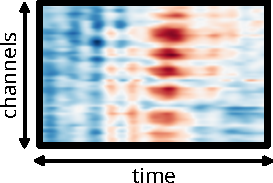
\includegraphics[width=\textwidth]{figures/bttda/tensor_st.pdf}
%  \end{minipage}\hfill%
%  \begin{minipage}[c]{.4\textwidth}
%    \centering
%    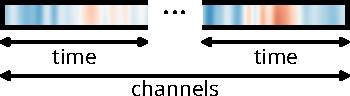
\includegraphics[width=\textwidth]{figures/bttda/tensor_flat.pdf}
%  \end{minipage}
%\end{frame}
%
%
%\begin{frame}[c]
%	\frametitle{Higher-order discriminant analysis}
%	\centering
%	\begin{tikzpicture}[y=-1cm]
%		\TensorThree{$\ten{X}$}{}{}{}{2}{2}{1}
%		\begin{scope}[shift={(-1.1,0)}]
%			\TensorTwo{$\mat{W}_1$}{}{}{1}{2}
%		\end{scope}
%		\begin{scope}[shift={(0,2.1)}]
%			\TensorTwo{$\mat{W}_2$}{}{}{2}{1}
%		\end{scope}
%		\node at (3.3,.5, 2) {$=$};
%		\begin{scope}[shift={(4,0)}]
%			\TensorThree{$\ten{G}$}{}{}{$N$}{1}{1}{1}
%		\end{scope}
%	\end{tikzpicture}
%
%	\bigskip
%
%  $\ten{G} = \ten{X}\times_1\mat{W}_1\cdots\times_{K-1}\mat{W}_{K-1}$ \\
%  s.t. $\ten{G}$ is maximally \emph{discriminant}
%	between classes.
%\end{frame}
%
%\begin{frame}[c]
%	\frametitle{HODA and the Tucker tensor core model}
%
%	\begin{minipage}{.4\linewidth}
%		\centering
%    \emph{Tucker} model
%
%		\bigskip
%
%
%		\begin{tikzpicture}[y=-1cm]
%			\begin{scope}[shift={(-1,0)}]
%				\TensorThree{$\ten{X}$}{}{}{}{1}{2}{1}
%				\node at (2.5,.5, 2) {$\rightarrow$};
%				\begin{scope}[shift={(3,0)}]
%					\TensorThree{$\ten{G}$}{}{}{}{1}{1}{1}
%				\end{scope}
%				\node at (4.1,1.1, 2) {$\downarrow$};
%				\begin{scope}[shift={(3,2)}]
%					\TensorTwo{\textit{clf}}{}{}{1.5}{.5}
%				\end{scope}
%			\end{scope}
%		\end{tikzpicture}
%	\end{minipage}\hfill%
%	\begin{minipage}{.5\linewidth}
%		Strong assumptions\\
%		on data structure
%		\begin{itemize}
%			\item[\textcolor{mygreen}{+}] Efficient
%			\item[\textcolor{mygreen}{+}] Regularizing constraints
%			\item[\textcolor{mygreen}{+}] Increased flexibility
%				\smallskip
%
%      \item[\textcolor{myred}{--}] \sout{Redundant features}
%      \item[\textcolor{myred}{--}] \sout{More parameters to tune}
%		\end{itemize}
%	\end{minipage}
%\end{frame}
%
%\begin{frame}[c]
%	\frametitle{Towards a Block-Term Tensor model}
%	\begin{minipage}{.4\linewidth}
%		\centering
%		\textbf{Tucker} model
%
%		\bigskip
%
%		\begin{tikzpicture}[y=-1cm]
%			\begin{scope}[shift={(-1,0)}]
%				\TensorThree{$\ten{X}$}{}{}{}{1}{2}{1}
%				\node at (2.5,.5, 2) {$\rightarrow$};
%				\begin{scope}[shift={(3,0)}]
%					\TensorThree{$\ten{G}$}{}{}{}{1}{1}{1}
%				\end{scope}
%				\node at (4.1,1.1, 2) {$\downarrow$};
%				\begin{scope}[shift={(3,2)}]
%					\TensorTwo{\textit{clf}}{}{}{1.5}{.5}
%				\end{scope}
%			\end{scope}
%		\end{tikzpicture}
%	\end{minipage}\vline%
%	\begin{minipage}{.6\linewidth}
%		\centering
%		\emph{Block-Term Tensor} model
%
%		\bigskip
%
%
%		\begin{tikzpicture}[y=-1cm]
%			\begin{scope}[shift={(-1,0)}]
%				\TensorThree{$\ten{X}$}{}{}{}{1}{2}{1}
%				\node at (2.5,.5, 2) {$\rightarrow$};
%				\begin{scope}[shift={(3,0)}]
%					\TensorThree{$\ten{G}^{(1)}$}{}{}{}{1}{1}{1}
%				\end{scope}
%				\node at (5.5,.5,2) {$,\cdots,$};
%				\begin{scope}[shift={(6,0)}]
%					\TensorThree{$\ten{G}^{(B)}$}{}{}{}{1}{1}{1}
%				\end{scope}
%				\node at (4.1,1.1, 2) {$\downarrow$};
%				\node at (5.6,1.1, 2) {$\downarrow$};
%				\node at (7.1,1.1, 2) {$\downarrow$};
%				\begin{scope}[shift={(3,2)}]
%					\TensorTwo{\textit{clf}}{}{}{4.5}{.5}
%				\end{scope}
%			\end{scope}
%		\end{tikzpicture}
%
%	\end{minipage}
%\end{frame}
%
%\begin{frame}[c]
%	\frametitle{Block-term Tensor Discriminant Analysis}
%
%	\begin{minipage}{.6\linewidth}
%    \centering
%    \emph{Block-term Tensor} model
%
%		\bigskip
%
%    \raggedright
%		\begin{tikzpicture}[y=-1cm]
%			\begin{scope}[shift={(-1,0)}]
%				\TensorThree{$\ten{X}$}{}{}{}{1}{2}{1}
%				\node at (2.5,.5, 2) {$\rightarrow$};
%				\begin{scope}[shift={(3,0)}]
%					\TensorThree{$\ten{G}^{(1)}$}{}{}{}{1}{1}{1}
%				\end{scope}
%				\node at (5.5,.5,2) {$,\cdots,$};
%				\begin{scope}[shift={(6,0)}]
%					\TensorThree{$\ten{G}^{(B)}$}{}{}{}{1}{1}{1}
%				\end{scope}
%				\node at (4.1,1.1, 2) {$\downarrow$};
%				\node at (5.6,1.1, 2) {$\downarrow$};
%				\node at (7.1,1.1, 2) {$\downarrow$};
%				\begin{scope}[shift={(3,2)}]
%					\TensorTwo{\textit{clf}}{}{}{4.5}{.5}
%				\end{scope}
%			\end{scope}
%		\end{tikzpicture}
%	\end{minipage}\hfill%
%	\begin{minipage}{.4\linewidth}
%		Weaker assumptions\\
%		on data structure
%		\begin{itemize}
%
%			\item[\textcolor{mygreen}{+}] Efficient
%			\item[\textcolor{mygreen}{+}] Regularizing constraints
%				\smallskip
%
%      \item[\textcolor{myred}{--}] \sout{Manual rank selection}
%      \item[\textcolor{myred}{--}] \sout{Redundant features}
%      \item[\textcolor{myred}{--}] \sout{Cannot model full covariance structure}
%		\end{itemize}
%	\end{minipage}
%\end{frame}
%
%\begin{frame}[c]
%	\frametitle{Block-term tensor model through deflation}
%	\centering
%	\begin{tikzpicture}[y=-1cm]
%		\TensorThree{$\ten{X}$}{}{}{}{2}{2}{1}
%		\node at (3.3,.5, 2) {$\cong$};
%		\begin{scope}[shift={(6,0)}]
%			\TensorThree{$\ten{G}^{(1)}$}{}{}{}{1}{1}{1}
%		\end{scope}
%		\begin{scope}[shift={(3.9,0)}]
%			\TensorTwo{$\mat{A}_1^{(1)}$}{}{}{2}{1}
%		\end{scope}
%		\begin{scope}[shift={(6,1.1)}]
%			\TensorTwo{$\mat{A}_2^{(1)}$}{}{}{1}{2}
%		\end{scope}
%		\node at (8.6,.5, 2) {$+\cdots+$};
%		\begin{scope}[shift={(12,0)}]
%			\TensorThree{$\ten{G}^{(B)}$}{}{}{}{1}{1}{1}
%		\end{scope}
%		\begin{scope}[shift={(9.9,0)}]
%			\TensorTwo{$\mat{A}_1^{(B)}$}{}{}{2}{1}
%		\end{scope}
%		\begin{scope}[shift={(12,1.1)}]
%			\TensorTwo{$\mat{A}_2^{(B)}$}{}{}{1}{2}
%		\end{scope}
%	\end{tikzpicture}
%
%
%  \emph{Deflation} scheme:
%	%$$\ten{X}^{(0)} = \ten{X}$$
%	$$\ten{X}^{(b+1)} = \ten{X}^{(b)} -
%		\ten{G}^{(b)}\times_1\mat{A}_1^{(b)}\cdots\times_K\mat{A}_K^{(b)}$$
%\end{frame}
%
%\begin{frame}[c]
%  \frametitle{BTTDA oupterforms HODA \\ on benchmark datasets}
%  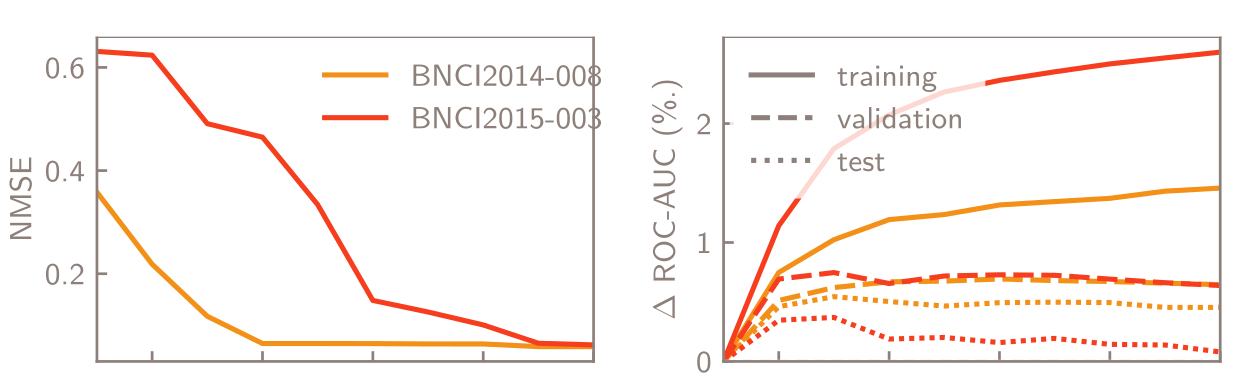
\includegraphics[width=.7\textwidth]{figures/bttda/blocks.png}%
%  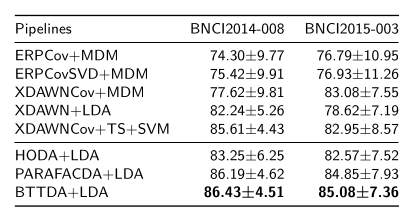
\includegraphics[width=.3\textwidth]{figures/bttda/results_table.png}
%
%\end{frame}
%
%\section{\textbf{C2}: Gaze-independent ERP decoding}
%\tocframe
%\begin{frame}
%  \frametitle{Covert attention ERP \\ data collection}
%  \begin{minipage}{.45\textwidth}
%    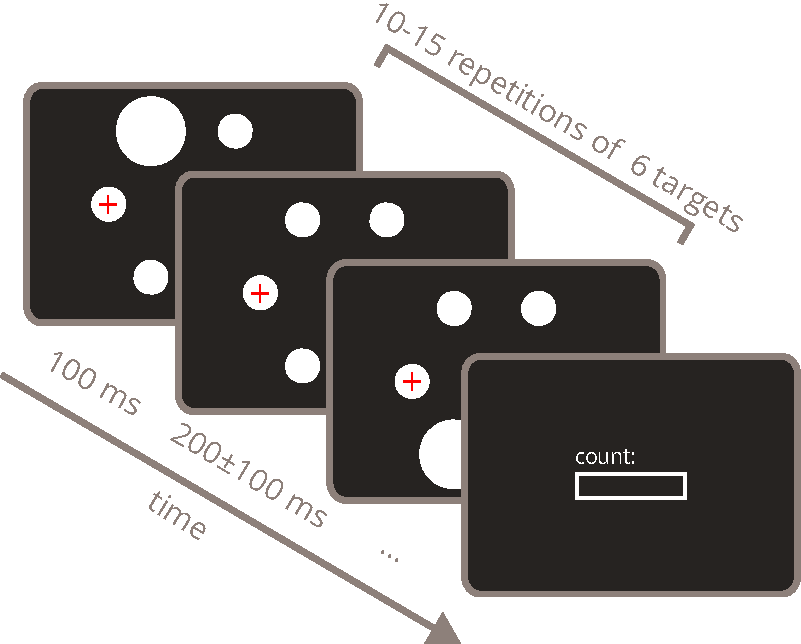
\includegraphics[width=\textwidth]{figures/covert/timeline.pdf}
%  \end{minipage}\hfill%
%  \begin{minipage}{.45\textwidth}
%     CVSA-ERP dataset
%     \begin{itemize}
%       \item $N=15$
%       \item ISI=$300\pm100$ ms
%       \item $\pm$11,25h recoded stimulation,
%       \item 3 conditions based on gaze and attention cue
%     \end{itemize}
%
%    \centering
%    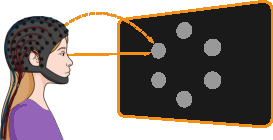
\includegraphics[width=.45\textwidth]{figures/covert/attention_overt.pdf}\hfill%
%    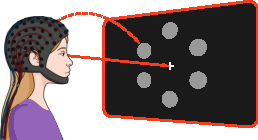
\includegraphics[width=.45\textwidth]{figures/covert/attention_covert.pdf}%
%    \bigskip
%
%    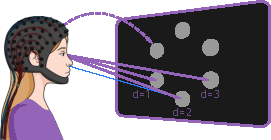
\includegraphics[width=.45\textwidth]{figures/covert/attention_split.pdf}
%  \end{minipage}
%\end{frame}
%
%\begin{frame}
%  \frametitle{Grand average ERPs}
%  TODO: grand average ERPs and F-scores
%\end{frame}
%
%\begin{frame}[c]
%  \frametitle{Latency jitter decreases performance \\ in covert and split
%  attention \tiny\cite{Arico2014}}
%  \begin{minipage}{.4\textwidth}
%    \centering
\small

\begin{tikzpicture}   % First subplot (low jitter) positioned relative to center
    \begin{axis}[
        at={(0,0)}, % Adjust position to the left, closer to the center
        anchor=center,
        width=\textwidth, height=.7\textwidth,
        xmin=20, xmax=80,
        ymin=-0.1, ymax=1.1,
        axis lines=none, % Remove axes
        title={low jitter}, % Add title
        title style={yshift=-10pt, color=muteblack}, % Adjust title position to make it closer to the plot
        ]
        % Plot individual waveforms (low jitter) in darkgray
        \addplot[darkgray,domain=20:80,samples=100] {exp(-0.5*((x-50)/5)^2)};
        \addplot[darkgray,domain=20:80,samples=100] {exp(-0.5*((x-52)/5)^2)};
        \addplot[darkgray,domain=20:80,samples=100] {exp(-0.5*((x-48)/5)^2)};
        \addplot[darkgray,domain=20:80,samples=100] {exp(-0.5*((x-51)/5)^2)};
        \addplot[darkgray,domain=20:80,samples=100] {exp(-0.5*((x-49)/5)^2)};

        % Plot average waveform (low jitter) in accent1 color, very thick
        \addplot[ultra thick,accent1,domain=20:80,samples=100] {exp(-0.5*((x-50)/5)^2)};
    \end{axis}
\end{tikzpicture}
\bigskip

\begin{tikzpicture}

   % Second subplot (high jitter) positioned relative to center
   \begin{axis}[
      at={(0.55\textwidth,0)}, % Adjust position to the left, closer to the center
       anchor=center,
        width=\textwidth, height=.7\textwidth,
       xmin=20, xmax=80,
       ymin=-0.1, ymax=1.1,
       axis lines=none, % Remove axes
       title={high jitter}, % Add title
       title style={yshift=-10pt, color=muteblack}, % Adjust title position to make it closer to the plot
       ]
       % Plot individual waveforms (high jitter) in darkgray
       \addplot[darkgray,domain=20:80,samples=100] {exp(-0.5*((x-45)/5)^2)};
       \addplot[darkgray,domain=20:80,samples=100] {exp(-0.5*((x-55)/5)^2)};
       \addplot[darkgray,domain=20:80,samples=100] {exp(-0.5*((x-40)/5)^2)};
       \addplot[darkgray,domain=20:80,samples=100] {exp(-0.5*((x-60)/5)^2)};
       \addplot[darkgray,domain=20:80,samples=100] {exp(-0.5*((x-50)/5)^2)};

       % Plot average waveform (high jitter) in accent1 color, very thick
       \addplot[ultra thick,accent1,domain=20:80,samples=100] {0.2*(exp(-0.5*((x-45)/5)^2) + exp(-0.5*((x-55)/5)^2) + exp(-0.5*((x-40)/5)^2) + exp(-0.5*((x-60)/5)^2) + exp(-0.5*((x-50)/5)^2))};
   \end{axis}
\end{tikzpicture}%
\bigskip

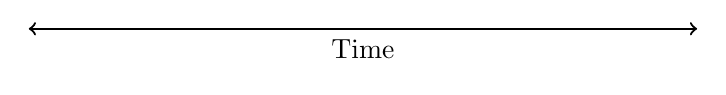
\begin{tikzpicture}
    % Draw the bottom horizontal axis
    \draw[thick,<->] (-0.35\textwidth,-1) -- (.35\textwidth,-1) node[pos=0.5,below] {Time};
\end{tikzpicture}
%\vspace{-5cm}

%  \end{minipage}\hfill%
%  \begin{minipage}{.55\textwidth}
%    \hspace{-0.24572736754045163in}
%%% Creator: Matplotlib, PGF backend
%%
%% To include the figure in your LaTeX document, write
%%   \input{<filename>.pgf}
%%
%% Make sure the required packages are loaded in your preamble
%%   \usepackage{pgf}
%%
%% Also ensure that all the required font packages are loaded; for instance,
%% the lmodern package is sometimes necessary when using math font.
%%   \usepackage{lmodern}
%%
%% Figures using additional raster images can only be included by \input if
%% they are in the same directory as the main LaTeX file. For loading figures
%% from other directories you can use the `import` package
%%   \usepackage{import}
%%
%% and then include the figures with
%%   \import{<path to file>}{<filename>.pgf}
%%
%% Matplotlib used the following preamble
%%   \def\mathdefault#1{#1}
%%   \everymath=\expandafter{\the\everymath\displaystyle}
%%
%%   \ifdefined\pdftexversion\else  % non-pdftex case.
%%     \usepackage{fontspec}
%%   \fi
%%   \makeatletter\@ifpackageloaded{underscore}{}{\usepackage[strings]{underscore}}\makeatother
%%
\begingroup%
\makeatletter%
\begin{pgfpicture}%
\pgfpathrectangle{\pgfpointorigin}{\pgfqpoint{2.997033in}{1.668849in}}%
\pgfusepath{use as bounding box, clip}%
\begin{pgfscope}%
\pgfsetbuttcap%
\pgfsetmiterjoin%
\pgfsetlinewidth{0.000000pt}%
\definecolor{currentstroke}{rgb}{1.000000,1.000000,1.000000}%
\pgfsetstrokecolor{currentstroke}%
\pgfsetstrokeopacity{0.000000}%
\pgfsetdash{}{0pt}%
\pgfpathmoveto{\pgfqpoint{0.000000in}{0.000000in}}%
\pgfpathlineto{\pgfqpoint{2.997033in}{0.000000in}}%
\pgfpathlineto{\pgfqpoint{2.997033in}{1.668849in}}%
\pgfpathlineto{\pgfqpoint{0.000000in}{1.668849in}}%
\pgfpathlineto{\pgfqpoint{0.000000in}{0.000000in}}%
\pgfpathclose%
\pgfusepath{}%
\end{pgfscope}%
\begin{pgfscope}%
\pgfsetbuttcap%
\pgfsetmiterjoin%
\definecolor{currentfill}{rgb}{1.000000,1.000000,1.000000}%
\pgfsetfillcolor{currentfill}%
\pgfsetlinewidth{0.000000pt}%
\definecolor{currentstroke}{rgb}{0.000000,0.000000,0.000000}%
\pgfsetstrokecolor{currentstroke}%
\pgfsetstrokeopacity{0.000000}%
\pgfsetdash{}{0pt}%
\pgfpathmoveto{\pgfqpoint{0.229167in}{0.470139in}}%
\pgfpathlineto{\pgfqpoint{2.146685in}{0.470139in}}%
\pgfpathlineto{\pgfqpoint{2.146685in}{1.608911in}}%
\pgfpathlineto{\pgfqpoint{0.229167in}{1.608911in}}%
\pgfpathlineto{\pgfqpoint{0.229167in}{0.470139in}}%
\pgfpathclose%
\pgfusepath{fill}%
\end{pgfscope}%
\begin{pgfscope}%
\pgfpathrectangle{\pgfqpoint{0.229167in}{0.470139in}}{\pgfqpoint{1.917519in}{1.138772in}}%
\pgfusepath{clip}%
\pgfsetbuttcap%
\pgfsetmiterjoin%
\definecolor{currentfill}{rgb}{0.842157,0.553922,0.200980}%
\pgfsetfillcolor{currentfill}%
\pgfsetlinewidth{0.000000pt}%
\definecolor{currentstroke}{rgb}{0.000000,0.000000,0.000000}%
\pgfsetstrokecolor{currentstroke}%
\pgfsetstrokeopacity{0.000000}%
\pgfsetdash{}{0pt}%
\pgfpathmoveto{\pgfqpoint{0.316327in}{0.470139in}}%
\pgfpathlineto{\pgfqpoint{0.606860in}{0.470139in}}%
\pgfpathlineto{\pgfqpoint{0.606860in}{0.705246in}}%
\pgfpathlineto{\pgfqpoint{0.316327in}{0.705246in}}%
\pgfpathlineto{\pgfqpoint{0.316327in}{0.470139in}}%
\pgfpathclose%
\pgfusepath{fill}%
\end{pgfscope}%
\begin{pgfscope}%
\pgfpathrectangle{\pgfqpoint{0.229167in}{0.470139in}}{\pgfqpoint{1.917519in}{1.138772in}}%
\pgfusepath{clip}%
\pgfsetbuttcap%
\pgfsetmiterjoin%
\definecolor{currentfill}{rgb}{0.858824,0.314706,0.223529}%
\pgfsetfillcolor{currentfill}%
\pgfsetlinewidth{0.000000pt}%
\definecolor{currentstroke}{rgb}{0.000000,0.000000,0.000000}%
\pgfsetstrokecolor{currentstroke}%
\pgfsetstrokeopacity{0.000000}%
\pgfsetdash{}{0pt}%
\pgfpathmoveto{\pgfqpoint{0.679493in}{0.470139in}}%
\pgfpathlineto{\pgfqpoint{0.970026in}{0.470139in}}%
\pgfpathlineto{\pgfqpoint{0.970026in}{1.007696in}}%
\pgfpathlineto{\pgfqpoint{0.679493in}{1.007696in}}%
\pgfpathlineto{\pgfqpoint{0.679493in}{0.470139in}}%
\pgfpathclose%
\pgfusepath{fill}%
\end{pgfscope}%
\begin{pgfscope}%
\pgfpathrectangle{\pgfqpoint{0.229167in}{0.470139in}}{\pgfqpoint{1.917519in}{1.138772in}}%
\pgfusepath{clip}%
\pgfsetbuttcap%
\pgfsetmiterjoin%
\definecolor{currentfill}{rgb}{0.464706,0.320588,0.573529}%
\pgfsetfillcolor{currentfill}%
\pgfsetlinewidth{0.000000pt}%
\definecolor{currentstroke}{rgb}{0.000000,0.000000,0.000000}%
\pgfsetstrokecolor{currentstroke}%
\pgfsetstrokeopacity{0.000000}%
\pgfsetdash{}{0pt}%
\pgfpathmoveto{\pgfqpoint{1.042660in}{0.470139in}}%
\pgfpathlineto{\pgfqpoint{1.333193in}{0.470139in}}%
\pgfpathlineto{\pgfqpoint{1.333193in}{0.979341in}}%
\pgfpathlineto{\pgfqpoint{1.042660in}{0.979341in}}%
\pgfpathlineto{\pgfqpoint{1.042660in}{0.470139in}}%
\pgfpathclose%
\pgfusepath{fill}%
\end{pgfscope}%
\begin{pgfscope}%
\pgfpathrectangle{\pgfqpoint{0.229167in}{0.470139in}}{\pgfqpoint{1.917519in}{1.138772in}}%
\pgfusepath{clip}%
\pgfsetbuttcap%
\pgfsetmiterjoin%
\definecolor{currentfill}{rgb}{0.464706,0.320588,0.573529}%
\pgfsetfillcolor{currentfill}%
\pgfsetlinewidth{0.000000pt}%
\definecolor{currentstroke}{rgb}{0.000000,0.000000,0.000000}%
\pgfsetstrokecolor{currentstroke}%
\pgfsetstrokeopacity{0.000000}%
\pgfsetdash{}{0pt}%
\pgfpathmoveto{\pgfqpoint{1.405826in}{0.470139in}}%
\pgfpathlineto{\pgfqpoint{1.696359in}{0.470139in}}%
\pgfpathlineto{\pgfqpoint{1.696359in}{1.012421in}}%
\pgfpathlineto{\pgfqpoint{1.405826in}{1.012421in}}%
\pgfpathlineto{\pgfqpoint{1.405826in}{0.470139in}}%
\pgfpathclose%
\pgfusepath{fill}%
\end{pgfscope}%
\begin{pgfscope}%
\pgfpathrectangle{\pgfqpoint{0.229167in}{0.470139in}}{\pgfqpoint{1.917519in}{1.138772in}}%
\pgfusepath{clip}%
\pgfsetbuttcap%
\pgfsetmiterjoin%
\definecolor{currentfill}{rgb}{0.464706,0.320588,0.573529}%
\pgfsetfillcolor{currentfill}%
\pgfsetlinewidth{0.000000pt}%
\definecolor{currentstroke}{rgb}{0.000000,0.000000,0.000000}%
\pgfsetstrokecolor{currentstroke}%
\pgfsetstrokeopacity{0.000000}%
\pgfsetdash{}{0pt}%
\pgfpathmoveto{\pgfqpoint{1.768992in}{0.470139in}}%
\pgfpathlineto{\pgfqpoint{2.059526in}{0.470139in}}%
\pgfpathlineto{\pgfqpoint{2.059526in}{0.975797in}}%
\pgfpathlineto{\pgfqpoint{1.768992in}{0.975797in}}%
\pgfpathlineto{\pgfqpoint{1.768992in}{0.470139in}}%
\pgfpathclose%
\pgfusepath{fill}%
\end{pgfscope}%
\begin{pgfscope}%
\pgfsetbuttcap%
\pgfsetroundjoin%
\definecolor{currentfill}{rgb}{0.552941,0.501961,0.478431}%
\pgfsetfillcolor{currentfill}%
\pgfsetlinewidth{0.803000pt}%
\definecolor{currentstroke}{rgb}{0.552941,0.501961,0.478431}%
\pgfsetstrokecolor{currentstroke}%
\pgfsetdash{}{0pt}%
\pgfsys@defobject{currentmarker}{\pgfqpoint{0.000000in}{0.000000in}}{\pgfqpoint{0.000000in}{0.041667in}}{%
\pgfpathmoveto{\pgfqpoint{0.000000in}{0.000000in}}%
\pgfpathlineto{\pgfqpoint{0.000000in}{0.041667in}}%
\pgfusepath{stroke,fill}%
}%
\begin{pgfscope}%
\pgfsys@transformshift{0.461593in}{0.470139in}%
\pgfsys@useobject{currentmarker}{}%
\end{pgfscope}%
\end{pgfscope}%
\begin{pgfscope}%
\definecolor{textcolor}{rgb}{0.552941,0.501961,0.478431}%
\pgfsetstrokecolor{textcolor}%
\pgfsetfillcolor{textcolor}%
\pgftext[x=0.461593in,y=0.421528in,,top]{\color{textcolor}{\sffamily\fontsize{9.000000}{10.800000}\selectfont\catcode`\^=\active\def^{\ifmmode\sp\else\^{}\fi}\catcode`\%=\active\def%{\%}overt}}%
\end{pgfscope}%
\begin{pgfscope}%
\pgfsetbuttcap%
\pgfsetroundjoin%
\definecolor{currentfill}{rgb}{0.552941,0.501961,0.478431}%
\pgfsetfillcolor{currentfill}%
\pgfsetlinewidth{0.803000pt}%
\definecolor{currentstroke}{rgb}{0.552941,0.501961,0.478431}%
\pgfsetstrokecolor{currentstroke}%
\pgfsetdash{}{0pt}%
\pgfsys@defobject{currentmarker}{\pgfqpoint{0.000000in}{0.000000in}}{\pgfqpoint{0.000000in}{0.041667in}}{%
\pgfpathmoveto{\pgfqpoint{0.000000in}{0.000000in}}%
\pgfpathlineto{\pgfqpoint{0.000000in}{0.041667in}}%
\pgfusepath{stroke,fill}%
}%
\begin{pgfscope}%
\pgfsys@transformshift{0.824760in}{0.470139in}%
\pgfsys@useobject{currentmarker}{}%
\end{pgfscope}%
\end{pgfscope}%
\begin{pgfscope}%
\definecolor{textcolor}{rgb}{0.552941,0.501961,0.478431}%
\pgfsetstrokecolor{textcolor}%
\pgfsetfillcolor{textcolor}%
\pgftext[x=0.824760in,y=0.421528in,,top]{\color{textcolor}{\sffamily\fontsize{9.000000}{10.800000}\selectfont\catcode`\^=\active\def^{\ifmmode\sp\else\^{}\fi}\catcode`\%=\active\def%{\%}covert}}%
\end{pgfscope}%
\begin{pgfscope}%
\pgfsetbuttcap%
\pgfsetroundjoin%
\definecolor{currentfill}{rgb}{0.552941,0.501961,0.478431}%
\pgfsetfillcolor{currentfill}%
\pgfsetlinewidth{0.803000pt}%
\definecolor{currentstroke}{rgb}{0.552941,0.501961,0.478431}%
\pgfsetstrokecolor{currentstroke}%
\pgfsetdash{}{0pt}%
\pgfsys@defobject{currentmarker}{\pgfqpoint{0.000000in}{0.000000in}}{\pgfqpoint{0.000000in}{0.041667in}}{%
\pgfpathmoveto{\pgfqpoint{0.000000in}{0.000000in}}%
\pgfpathlineto{\pgfqpoint{0.000000in}{0.041667in}}%
\pgfusepath{stroke,fill}%
}%
\begin{pgfscope}%
\pgfsys@transformshift{1.187926in}{0.470139in}%
\pgfsys@useobject{currentmarker}{}%
\end{pgfscope}%
\end{pgfscope}%
\begin{pgfscope}%
\definecolor{textcolor}{rgb}{0.552941,0.501961,0.478431}%
\pgfsetstrokecolor{textcolor}%
\pgfsetfillcolor{textcolor}%
\pgftext[x=1.076257in, y=0.334722in, left, base]{\color{textcolor}{\sffamily\fontsize{9.000000}{10.800000}\selectfont\catcode`\^=\active\def^{\ifmmode\sp\else\^{}\fi}\catcode`\%=\active\def%{\%}split}}%
\end{pgfscope}%
\begin{pgfscope}%
\definecolor{textcolor}{rgb}{0.552941,0.501961,0.478431}%
\pgfsetstrokecolor{textcolor}%
\pgfsetfillcolor{textcolor}%
\pgftext[x=0.986917in, y=0.197917in, left, base]{\color{textcolor}{\sffamily\fontsize{9.000000}{10.800000}\selectfont\catcode`\^=\active\def^{\ifmmode\sp\else\^{}\fi}\catcode`\%=\active\def%{\%}($d=1$)}}%
\end{pgfscope}%
\begin{pgfscope}%
\pgfsetbuttcap%
\pgfsetroundjoin%
\definecolor{currentfill}{rgb}{0.552941,0.501961,0.478431}%
\pgfsetfillcolor{currentfill}%
\pgfsetlinewidth{0.803000pt}%
\definecolor{currentstroke}{rgb}{0.552941,0.501961,0.478431}%
\pgfsetstrokecolor{currentstroke}%
\pgfsetdash{}{0pt}%
\pgfsys@defobject{currentmarker}{\pgfqpoint{0.000000in}{0.000000in}}{\pgfqpoint{0.000000in}{0.041667in}}{%
\pgfpathmoveto{\pgfqpoint{0.000000in}{0.000000in}}%
\pgfpathlineto{\pgfqpoint{0.000000in}{0.041667in}}%
\pgfusepath{stroke,fill}%
}%
\begin{pgfscope}%
\pgfsys@transformshift{1.551093in}{0.470139in}%
\pgfsys@useobject{currentmarker}{}%
\end{pgfscope}%
\end{pgfscope}%
\begin{pgfscope}%
\definecolor{textcolor}{rgb}{0.552941,0.501961,0.478431}%
\pgfsetstrokecolor{textcolor}%
\pgfsetfillcolor{textcolor}%
\pgftext[x=1.439423in, y=0.334722in, left, base]{\color{textcolor}{\sffamily\fontsize{9.000000}{10.800000}\selectfont\catcode`\^=\active\def^{\ifmmode\sp\else\^{}\fi}\catcode`\%=\active\def%{\%}split}}%
\end{pgfscope}%
\begin{pgfscope}%
\definecolor{textcolor}{rgb}{0.552941,0.501961,0.478431}%
\pgfsetstrokecolor{textcolor}%
\pgfsetfillcolor{textcolor}%
\pgftext[x=1.350083in, y=0.197917in, left, base]{\color{textcolor}{\sffamily\fontsize{9.000000}{10.800000}\selectfont\catcode`\^=\active\def^{\ifmmode\sp\else\^{}\fi}\catcode`\%=\active\def%{\%}($d=2$)}}%
\end{pgfscope}%
\begin{pgfscope}%
\pgfsetbuttcap%
\pgfsetroundjoin%
\definecolor{currentfill}{rgb}{0.552941,0.501961,0.478431}%
\pgfsetfillcolor{currentfill}%
\pgfsetlinewidth{0.803000pt}%
\definecolor{currentstroke}{rgb}{0.552941,0.501961,0.478431}%
\pgfsetstrokecolor{currentstroke}%
\pgfsetdash{}{0pt}%
\pgfsys@defobject{currentmarker}{\pgfqpoint{0.000000in}{0.000000in}}{\pgfqpoint{0.000000in}{0.041667in}}{%
\pgfpathmoveto{\pgfqpoint{0.000000in}{0.000000in}}%
\pgfpathlineto{\pgfqpoint{0.000000in}{0.041667in}}%
\pgfusepath{stroke,fill}%
}%
\begin{pgfscope}%
\pgfsys@transformshift{1.914259in}{0.470139in}%
\pgfsys@useobject{currentmarker}{}%
\end{pgfscope}%
\end{pgfscope}%
\begin{pgfscope}%
\definecolor{textcolor}{rgb}{0.552941,0.501961,0.478431}%
\pgfsetstrokecolor{textcolor}%
\pgfsetfillcolor{textcolor}%
\pgftext[x=1.802590in, y=0.334722in, left, base]{\color{textcolor}{\sffamily\fontsize{9.000000}{10.800000}\selectfont\catcode`\^=\active\def^{\ifmmode\sp\else\^{}\fi}\catcode`\%=\active\def%{\%}split}}%
\end{pgfscope}%
\begin{pgfscope}%
\definecolor{textcolor}{rgb}{0.552941,0.501961,0.478431}%
\pgfsetstrokecolor{textcolor}%
\pgfsetfillcolor{textcolor}%
\pgftext[x=1.713250in, y=0.197917in, left, base]{\color{textcolor}{\sffamily\fontsize{9.000000}{10.800000}\selectfont\catcode`\^=\active\def^{\ifmmode\sp\else\^{}\fi}\catcode`\%=\active\def%{\%}($d=3$)}}%
\end{pgfscope}%
\begin{pgfscope}%
\definecolor{textcolor}{rgb}{0.552941,0.501961,0.478431}%
\pgfsetstrokecolor{textcolor}%
\pgfsetfillcolor{textcolor}%
\pgftext[x=1.187926in,y=0.111111in,,top]{\color{textcolor}{\sffamily\fontsize{9.000000}{10.800000}\selectfont\catcode`\^=\active\def^{\ifmmode\sp\else\^{}\fi}\catcode`\%=\active\def%{\%}VSA condition}}%
\end{pgfscope}%
\begin{pgfscope}%
\pgfsetbuttcap%
\pgfsetroundjoin%
\definecolor{currentfill}{rgb}{0.552941,0.501961,0.478431}%
\pgfsetfillcolor{currentfill}%
\pgfsetlinewidth{0.803000pt}%
\definecolor{currentstroke}{rgb}{0.552941,0.501961,0.478431}%
\pgfsetstrokecolor{currentstroke}%
\pgfsetdash{}{0pt}%
\pgfsys@defobject{currentmarker}{\pgfqpoint{0.000000in}{0.000000in}}{\pgfqpoint{0.041667in}{0.000000in}}{%
\pgfpathmoveto{\pgfqpoint{0.000000in}{0.000000in}}%
\pgfpathlineto{\pgfqpoint{0.041667in}{0.000000in}}%
\pgfusepath{stroke,fill}%
}%
\begin{pgfscope}%
\pgfsys@transformshift{0.229167in}{0.470139in}%
\pgfsys@useobject{currentmarker}{}%
\end{pgfscope}%
\end{pgfscope}%
\begin{pgfscope}%
\pgfsetbuttcap%
\pgfsetroundjoin%
\definecolor{currentfill}{rgb}{0.552941,0.501961,0.478431}%
\pgfsetfillcolor{currentfill}%
\pgfsetlinewidth{0.803000pt}%
\definecolor{currentstroke}{rgb}{0.552941,0.501961,0.478431}%
\pgfsetstrokecolor{currentstroke}%
\pgfsetdash{}{0pt}%
\pgfsys@defobject{currentmarker}{\pgfqpoint{0.000000in}{0.000000in}}{\pgfqpoint{0.041667in}{0.000000in}}{%
\pgfpathmoveto{\pgfqpoint{0.000000in}{0.000000in}}%
\pgfpathlineto{\pgfqpoint{0.041667in}{0.000000in}}%
\pgfusepath{stroke,fill}%
}%
\begin{pgfscope}%
\pgfsys@transformshift{0.229167in}{0.821371in}%
\pgfsys@useobject{currentmarker}{}%
\end{pgfscope}%
\end{pgfscope}%
\begin{pgfscope}%
\pgfsetbuttcap%
\pgfsetroundjoin%
\definecolor{currentfill}{rgb}{0.552941,0.501961,0.478431}%
\pgfsetfillcolor{currentfill}%
\pgfsetlinewidth{0.803000pt}%
\definecolor{currentstroke}{rgb}{0.552941,0.501961,0.478431}%
\pgfsetstrokecolor{currentstroke}%
\pgfsetdash{}{0pt}%
\pgfsys@defobject{currentmarker}{\pgfqpoint{0.000000in}{0.000000in}}{\pgfqpoint{0.041667in}{0.000000in}}{%
\pgfpathmoveto{\pgfqpoint{0.000000in}{0.000000in}}%
\pgfpathlineto{\pgfqpoint{0.041667in}{0.000000in}}%
\pgfusepath{stroke,fill}%
}%
\begin{pgfscope}%
\pgfsys@transformshift{0.229167in}{1.172602in}%
\pgfsys@useobject{currentmarker}{}%
\end{pgfscope}%
\end{pgfscope}%
\begin{pgfscope}%
\pgfsetbuttcap%
\pgfsetroundjoin%
\definecolor{currentfill}{rgb}{0.552941,0.501961,0.478431}%
\pgfsetfillcolor{currentfill}%
\pgfsetlinewidth{0.803000pt}%
\definecolor{currentstroke}{rgb}{0.552941,0.501961,0.478431}%
\pgfsetstrokecolor{currentstroke}%
\pgfsetdash{}{0pt}%
\pgfsys@defobject{currentmarker}{\pgfqpoint{0.000000in}{0.000000in}}{\pgfqpoint{0.041667in}{0.000000in}}{%
\pgfpathmoveto{\pgfqpoint{0.000000in}{0.000000in}}%
\pgfpathlineto{\pgfqpoint{0.041667in}{0.000000in}}%
\pgfusepath{stroke,fill}%
}%
\begin{pgfscope}%
\pgfsys@transformshift{0.229167in}{1.523834in}%
\pgfsys@useobject{currentmarker}{}%
\end{pgfscope}%
\end{pgfscope}%
\begin{pgfscope}%
\definecolor{textcolor}{rgb}{0.552941,0.501961,0.478431}%
\pgfsetstrokecolor{textcolor}%
\pgfsetfillcolor{textcolor}%
\pgftext[x=0.125000in,y=1.039525in,,bottom,rotate=90.000000]{\color{textcolor}{\sffamily\fontsize{9.000000}{10.800000}\selectfont\catcode`\^=\active\def^{\ifmmode\sp\else\^{}\fi}\catcode`\%=\active\def%{\%}Target latency IQR (s)}}%
\end{pgfscope}%
\begin{pgfscope}%
\pgfpathrectangle{\pgfqpoint{0.229167in}{0.470139in}}{\pgfqpoint{1.917519in}{1.138772in}}%
\pgfusepath{clip}%
\pgfsetrectcap%
\pgfsetroundjoin%
\pgfsetlinewidth{2.258437pt}%
\definecolor{currentstroke}{rgb}{0.260000,0.260000,0.260000}%
\pgfsetstrokecolor{currentstroke}%
\pgfsetdash{}{0pt}%
\pgfpathmoveto{\pgfqpoint{0.461593in}{0.635541in}}%
\pgfpathlineto{\pgfqpoint{0.461593in}{0.784403in}}%
\pgfusepath{stroke}%
\end{pgfscope}%
\begin{pgfscope}%
\pgfpathrectangle{\pgfqpoint{0.229167in}{0.470139in}}{\pgfqpoint{1.917519in}{1.138772in}}%
\pgfusepath{clip}%
\pgfsetrectcap%
\pgfsetroundjoin%
\pgfsetlinewidth{2.258437pt}%
\definecolor{currentstroke}{rgb}{0.260000,0.260000,0.260000}%
\pgfsetstrokecolor{currentstroke}%
\pgfsetdash{}{0pt}%
\pgfpathmoveto{\pgfqpoint{0.824760in}{0.978159in}}%
\pgfpathlineto{\pgfqpoint{0.824760in}{1.033687in}}%
\pgfusepath{stroke}%
\end{pgfscope}%
\begin{pgfscope}%
\pgfpathrectangle{\pgfqpoint{0.229167in}{0.470139in}}{\pgfqpoint{1.917519in}{1.138772in}}%
\pgfusepath{clip}%
\pgfsetrectcap%
\pgfsetroundjoin%
\pgfsetlinewidth{2.258437pt}%
\definecolor{currentstroke}{rgb}{0.260000,0.260000,0.260000}%
\pgfsetstrokecolor{currentstroke}%
\pgfsetdash{}{0pt}%
\pgfpathmoveto{\pgfqpoint{1.187926in}{0.928539in}}%
\pgfpathlineto{\pgfqpoint{1.187926in}{1.028961in}}%
\pgfusepath{stroke}%
\end{pgfscope}%
\begin{pgfscope}%
\pgfpathrectangle{\pgfqpoint{0.229167in}{0.470139in}}{\pgfqpoint{1.917519in}{1.138772in}}%
\pgfusepath{clip}%
\pgfsetrectcap%
\pgfsetroundjoin%
\pgfsetlinewidth{2.258437pt}%
\definecolor{currentstroke}{rgb}{0.260000,0.260000,0.260000}%
\pgfsetstrokecolor{currentstroke}%
\pgfsetdash{}{0pt}%
\pgfpathmoveto{\pgfqpoint{1.551093in}{0.954531in}}%
\pgfpathlineto{\pgfqpoint{1.551093in}{1.083308in}}%
\pgfusepath{stroke}%
\end{pgfscope}%
\begin{pgfscope}%
\pgfpathrectangle{\pgfqpoint{0.229167in}{0.470139in}}{\pgfqpoint{1.917519in}{1.138772in}}%
\pgfusepath{clip}%
\pgfsetrectcap%
\pgfsetroundjoin%
\pgfsetlinewidth{2.258437pt}%
\definecolor{currentstroke}{rgb}{0.260000,0.260000,0.260000}%
\pgfsetstrokecolor{currentstroke}%
\pgfsetdash{}{0pt}%
\pgfpathmoveto{\pgfqpoint{1.914259in}{0.940353in}}%
\pgfpathlineto{\pgfqpoint{1.914259in}{1.010088in}}%
\pgfusepath{stroke}%
\end{pgfscope}%
\begin{pgfscope}%
\pgfsetrectcap%
\pgfsetroundjoin%
\pgfsetlinewidth{1.003750pt}%
\definecolor{currentstroke}{rgb}{0.200000,0.200000,0.200000}%
\pgfsetstrokecolor{currentstroke}%
\pgfsetdash{}{0pt}%
\pgfpathmoveto{\pgfqpoint{0.461593in}{1.072317in}}%
\pgfpathlineto{\pgfqpoint{0.461593in}{1.136700in}}%
\pgfpathlineto{\pgfqpoint{0.824760in}{1.136700in}}%
\pgfpathlineto{\pgfqpoint{0.824760in}{1.072317in}}%
\pgfusepath{stroke}%
\end{pgfscope}%
\begin{pgfscope}%
\pgfsetrectcap%
\pgfsetroundjoin%
\pgfsetlinewidth{1.003750pt}%
\definecolor{currentstroke}{rgb}{0.200000,0.200000,0.200000}%
\pgfsetstrokecolor{currentstroke}%
\pgfsetdash{}{0pt}%
\pgfpathmoveto{\pgfqpoint{0.461593in}{1.203918in}}%
\pgfpathlineto{\pgfqpoint{0.461593in}{1.268301in}}%
\pgfpathlineto{\pgfqpoint{1.187926in}{1.268301in}}%
\pgfpathlineto{\pgfqpoint{1.187926in}{1.203918in}}%
\pgfusepath{stroke}%
\end{pgfscope}%
\begin{pgfscope}%
\pgfsetrectcap%
\pgfsetroundjoin%
\pgfsetlinewidth{1.003750pt}%
\definecolor{currentstroke}{rgb}{0.200000,0.200000,0.200000}%
\pgfsetstrokecolor{currentstroke}%
\pgfsetdash{}{0pt}%
\pgfpathmoveto{\pgfqpoint{0.461593in}{1.335519in}}%
\pgfpathlineto{\pgfqpoint{0.461593in}{1.399902in}}%
\pgfpathlineto{\pgfqpoint{1.551093in}{1.399902in}}%
\pgfpathlineto{\pgfqpoint{1.551093in}{1.335519in}}%
\pgfusepath{stroke}%
\end{pgfscope}%
\begin{pgfscope}%
\pgfsetrectcap%
\pgfsetroundjoin%
\pgfsetlinewidth{1.003750pt}%
\definecolor{currentstroke}{rgb}{0.200000,0.200000,0.200000}%
\pgfsetstrokecolor{currentstroke}%
\pgfsetdash{}{0pt}%
\pgfpathmoveto{\pgfqpoint{0.461593in}{1.467120in}}%
\pgfpathlineto{\pgfqpoint{0.461593in}{1.531503in}}%
\pgfpathlineto{\pgfqpoint{1.914259in}{1.531503in}}%
\pgfpathlineto{\pgfqpoint{1.914259in}{1.467120in}}%
\pgfusepath{stroke}%
\end{pgfscope}%
\begin{pgfscope}%
\pgfsetrectcap%
\pgfsetmiterjoin%
\pgfsetlinewidth{0.803000pt}%
\definecolor{currentstroke}{rgb}{0.552941,0.501961,0.478431}%
\pgfsetstrokecolor{currentstroke}%
\pgfsetdash{}{0pt}%
\pgfpathmoveto{\pgfqpoint{0.229167in}{0.470139in}}%
\pgfpathlineto{\pgfqpoint{0.229167in}{1.608911in}}%
\pgfusepath{stroke}%
\end{pgfscope}%
\begin{pgfscope}%
\pgfsetrectcap%
\pgfsetmiterjoin%
\pgfsetlinewidth{0.803000pt}%
\definecolor{currentstroke}{rgb}{0.552941,0.501961,0.478431}%
\pgfsetstrokecolor{currentstroke}%
\pgfsetdash{}{0pt}%
\pgfpathmoveto{\pgfqpoint{0.229167in}{0.470139in}}%
\pgfpathlineto{\pgfqpoint{2.146685in}{0.470139in}}%
\pgfusepath{stroke}%
\end{pgfscope}%
\begin{pgfscope}%
\definecolor{textcolor}{rgb}{0.552941,0.501961,0.478431}%
\pgfsetstrokecolor{textcolor}%
\pgfsetfillcolor{textcolor}%
\pgftext[x=0.643176in,y=1.150589in,,bottom]{\color{textcolor}{\sffamily\fontsize{10.000000}{12.000000}\selectfont\catcode`\^=\active\def^{\ifmmode\sp\else\^{}\fi}\catcode`\%=\active\def%{\%}***}}%
\end{pgfscope}%
\begin{pgfscope}%
\definecolor{textcolor}{rgb}{0.552941,0.501961,0.478431}%
\pgfsetstrokecolor{textcolor}%
\pgfsetfillcolor{textcolor}%
\pgftext[x=0.824760in,y=1.282190in,,bottom]{\color{textcolor}{\sffamily\fontsize{10.000000}{12.000000}\selectfont\catcode`\^=\active\def^{\ifmmode\sp\else\^{}\fi}\catcode`\%=\active\def%{\%}**}}%
\end{pgfscope}%
\begin{pgfscope}%
\definecolor{textcolor}{rgb}{0.552941,0.501961,0.478431}%
\pgfsetstrokecolor{textcolor}%
\pgfsetfillcolor{textcolor}%
\pgftext[x=1.006343in,y=1.413791in,,bottom]{\color{textcolor}{\sffamily\fontsize{10.000000}{12.000000}\selectfont\catcode`\^=\active\def^{\ifmmode\sp\else\^{}\fi}\catcode`\%=\active\def%{\%}**}}%
\end{pgfscope}%
\begin{pgfscope}%
\definecolor{textcolor}{rgb}{0.552941,0.501961,0.478431}%
\pgfsetstrokecolor{textcolor}%
\pgfsetfillcolor{textcolor}%
\pgftext[x=1.187926in,y=1.545392in,,bottom]{\color{textcolor}{\sffamily\fontsize{10.000000}{12.000000}\selectfont\catcode`\^=\active\def^{\ifmmode\sp\else\^{}\fi}\catcode`\%=\active\def%{\%}**}}%
\end{pgfscope}%
\begin{pgfscope}%
\pgfsetbuttcap%
\pgfsetmiterjoin%
\definecolor{currentfill}{rgb}{1.000000,1.000000,1.000000}%
\pgfsetfillcolor{currentfill}%
\pgfsetlinewidth{0.000000pt}%
\definecolor{currentstroke}{rgb}{0.000000,0.000000,0.000000}%
\pgfsetstrokecolor{currentstroke}%
\pgfsetstrokeopacity{0.000000}%
\pgfsetdash{}{0pt}%
\pgfpathmoveto{\pgfqpoint{2.230025in}{0.470139in}}%
\pgfpathlineto{\pgfqpoint{2.997033in}{0.470139in}}%
\pgfpathlineto{\pgfqpoint{2.997033in}{1.608911in}}%
\pgfpathlineto{\pgfqpoint{2.230025in}{1.608911in}}%
\pgfpathlineto{\pgfqpoint{2.230025in}{0.470139in}}%
\pgfpathclose%
\pgfusepath{fill}%
\end{pgfscope}%
\begin{pgfscope}%
\pgfpathrectangle{\pgfqpoint{2.230025in}{0.470139in}}{\pgfqpoint{0.767008in}{1.138772in}}%
\pgfusepath{clip}%
\pgfsetbuttcap%
\pgfsetmiterjoin%
\definecolor{currentfill}{rgb}{0.842157,0.553922,0.200980}%
\pgfsetfillcolor{currentfill}%
\pgfsetlinewidth{0.000000pt}%
\definecolor{currentstroke}{rgb}{0.000000,0.000000,0.000000}%
\pgfsetstrokecolor{currentstroke}%
\pgfsetstrokeopacity{0.000000}%
\pgfsetdash{}{0pt}%
\pgfpathmoveto{\pgfqpoint{2.264889in}{0.470139in}}%
\pgfpathlineto{\pgfqpoint{2.574792in}{0.470139in}}%
\pgfpathlineto{\pgfqpoint{2.574792in}{0.693995in}}%
\pgfpathlineto{\pgfqpoint{2.264889in}{0.693995in}}%
\pgfpathlineto{\pgfqpoint{2.264889in}{0.470139in}}%
\pgfpathclose%
\pgfusepath{fill}%
\end{pgfscope}%
\begin{pgfscope}%
\pgfpathrectangle{\pgfqpoint{2.230025in}{0.470139in}}{\pgfqpoint{0.767008in}{1.138772in}}%
\pgfusepath{clip}%
\pgfsetbuttcap%
\pgfsetmiterjoin%
\definecolor{currentfill}{rgb}{0.858824,0.314706,0.223529}%
\pgfsetfillcolor{currentfill}%
\pgfsetlinewidth{0.000000pt}%
\definecolor{currentstroke}{rgb}{0.000000,0.000000,0.000000}%
\pgfsetstrokecolor{currentstroke}%
\pgfsetstrokeopacity{0.000000}%
\pgfsetdash{}{0pt}%
\pgfpathmoveto{\pgfqpoint{2.652267in}{0.470139in}}%
\pgfpathlineto{\pgfqpoint{2.962169in}{0.470139in}}%
\pgfpathlineto{\pgfqpoint{2.962169in}{0.862361in}}%
\pgfpathlineto{\pgfqpoint{2.652267in}{0.862361in}}%
\pgfpathlineto{\pgfqpoint{2.652267in}{0.470139in}}%
\pgfpathclose%
\pgfusepath{fill}%
\end{pgfscope}%
\begin{pgfscope}%
\pgfsetbuttcap%
\pgfsetroundjoin%
\definecolor{currentfill}{rgb}{0.552941,0.501961,0.478431}%
\pgfsetfillcolor{currentfill}%
\pgfsetlinewidth{0.803000pt}%
\definecolor{currentstroke}{rgb}{0.552941,0.501961,0.478431}%
\pgfsetstrokecolor{currentstroke}%
\pgfsetdash{}{0pt}%
\pgfsys@defobject{currentmarker}{\pgfqpoint{0.000000in}{0.000000in}}{\pgfqpoint{0.000000in}{0.041667in}}{%
\pgfpathmoveto{\pgfqpoint{0.000000in}{0.000000in}}%
\pgfpathlineto{\pgfqpoint{0.000000in}{0.041667in}}%
\pgfusepath{stroke,fill}%
}%
\begin{pgfscope}%
\pgfsys@transformshift{2.419840in}{0.470139in}%
\pgfsys@useobject{currentmarker}{}%
\end{pgfscope}%
\end{pgfscope}%
\begin{pgfscope}%
\definecolor{textcolor}{rgb}{0.552941,0.501961,0.478431}%
\pgfsetstrokecolor{textcolor}%
\pgfsetfillcolor{textcolor}%
\pgftext[x=2.419840in,y=0.421528in,,top]{\color{textcolor}{\sffamily\fontsize{9.000000}{10.800000}\selectfont\catcode`\^=\active\def^{\ifmmode\sp\else\^{}\fi}\catcode`\%=\active\def%{\%}overt}}%
\end{pgfscope}%
\begin{pgfscope}%
\pgfsetbuttcap%
\pgfsetroundjoin%
\definecolor{currentfill}{rgb}{0.552941,0.501961,0.478431}%
\pgfsetfillcolor{currentfill}%
\pgfsetlinewidth{0.803000pt}%
\definecolor{currentstroke}{rgb}{0.552941,0.501961,0.478431}%
\pgfsetstrokecolor{currentstroke}%
\pgfsetdash{}{0pt}%
\pgfsys@defobject{currentmarker}{\pgfqpoint{0.000000in}{0.000000in}}{\pgfqpoint{0.000000in}{0.041667in}}{%
\pgfpathmoveto{\pgfqpoint{0.000000in}{0.000000in}}%
\pgfpathlineto{\pgfqpoint{0.000000in}{0.041667in}}%
\pgfusepath{stroke,fill}%
}%
\begin{pgfscope}%
\pgfsys@transformshift{2.807218in}{0.470139in}%
\pgfsys@useobject{currentmarker}{}%
\end{pgfscope}%
\end{pgfscope}%
\begin{pgfscope}%
\definecolor{textcolor}{rgb}{0.552941,0.501961,0.478431}%
\pgfsetstrokecolor{textcolor}%
\pgfsetfillcolor{textcolor}%
\pgftext[x=2.807218in,y=0.421528in,,top]{\color{textcolor}{\sffamily\fontsize{9.000000}{10.800000}\selectfont\catcode`\^=\active\def^{\ifmmode\sp\else\^{}\fi}\catcode`\%=\active\def%{\%}covert}}%
\end{pgfscope}%
\begin{pgfscope}%
\definecolor{textcolor}{rgb}{0.552941,0.501961,0.478431}%
\pgfsetstrokecolor{textcolor}%
\pgfsetfillcolor{textcolor}%
\pgftext[x=2.613529in,y=0.254861in,,top]{\color{textcolor}{\sffamily\fontsize{9.000000}{10.800000}\selectfont\catcode`\^=\active\def^{\ifmmode\sp\else\^{}\fi}\catcode`\%=\active\def%{\%}VSA condition}}%
\end{pgfscope}%
\begin{pgfscope}%
\pgfsetbuttcap%
\pgfsetroundjoin%
\definecolor{currentfill}{rgb}{0.552941,0.501961,0.478431}%
\pgfsetfillcolor{currentfill}%
\pgfsetlinewidth{0.803000pt}%
\definecolor{currentstroke}{rgb}{0.552941,0.501961,0.478431}%
\pgfsetstrokecolor{currentstroke}%
\pgfsetdash{}{0pt}%
\pgfsys@defobject{currentmarker}{\pgfqpoint{0.000000in}{0.000000in}}{\pgfqpoint{0.041667in}{0.000000in}}{%
\pgfpathmoveto{\pgfqpoint{0.000000in}{0.000000in}}%
\pgfpathlineto{\pgfqpoint{0.041667in}{0.000000in}}%
\pgfusepath{stroke,fill}%
}%
\begin{pgfscope}%
\pgfsys@transformshift{2.230025in}{0.470139in}%
\pgfsys@useobject{currentmarker}{}%
\end{pgfscope}%
\end{pgfscope}%
\begin{pgfscope}%
\pgfsetbuttcap%
\pgfsetroundjoin%
\definecolor{currentfill}{rgb}{0.552941,0.501961,0.478431}%
\pgfsetfillcolor{currentfill}%
\pgfsetlinewidth{0.803000pt}%
\definecolor{currentstroke}{rgb}{0.552941,0.501961,0.478431}%
\pgfsetstrokecolor{currentstroke}%
\pgfsetdash{}{0pt}%
\pgfsys@defobject{currentmarker}{\pgfqpoint{0.000000in}{0.000000in}}{\pgfqpoint{0.041667in}{0.000000in}}{%
\pgfpathmoveto{\pgfqpoint{0.000000in}{0.000000in}}%
\pgfpathlineto{\pgfqpoint{0.041667in}{0.000000in}}%
\pgfusepath{stroke,fill}%
}%
\begin{pgfscope}%
\pgfsys@transformshift{2.230025in}{0.821371in}%
\pgfsys@useobject{currentmarker}{}%
\end{pgfscope}%
\end{pgfscope}%
\begin{pgfscope}%
\pgfsetbuttcap%
\pgfsetroundjoin%
\definecolor{currentfill}{rgb}{0.552941,0.501961,0.478431}%
\pgfsetfillcolor{currentfill}%
\pgfsetlinewidth{0.803000pt}%
\definecolor{currentstroke}{rgb}{0.552941,0.501961,0.478431}%
\pgfsetstrokecolor{currentstroke}%
\pgfsetdash{}{0pt}%
\pgfsys@defobject{currentmarker}{\pgfqpoint{0.000000in}{0.000000in}}{\pgfqpoint{0.041667in}{0.000000in}}{%
\pgfpathmoveto{\pgfqpoint{0.000000in}{0.000000in}}%
\pgfpathlineto{\pgfqpoint{0.041667in}{0.000000in}}%
\pgfusepath{stroke,fill}%
}%
\begin{pgfscope}%
\pgfsys@transformshift{2.230025in}{1.172602in}%
\pgfsys@useobject{currentmarker}{}%
\end{pgfscope}%
\end{pgfscope}%
\begin{pgfscope}%
\pgfsetbuttcap%
\pgfsetroundjoin%
\definecolor{currentfill}{rgb}{0.552941,0.501961,0.478431}%
\pgfsetfillcolor{currentfill}%
\pgfsetlinewidth{0.803000pt}%
\definecolor{currentstroke}{rgb}{0.552941,0.501961,0.478431}%
\pgfsetstrokecolor{currentstroke}%
\pgfsetdash{}{0pt}%
\pgfsys@defobject{currentmarker}{\pgfqpoint{0.000000in}{0.000000in}}{\pgfqpoint{0.041667in}{0.000000in}}{%
\pgfpathmoveto{\pgfqpoint{0.000000in}{0.000000in}}%
\pgfpathlineto{\pgfqpoint{0.041667in}{0.000000in}}%
\pgfusepath{stroke,fill}%
}%
\begin{pgfscope}%
\pgfsys@transformshift{2.230025in}{1.523834in}%
\pgfsys@useobject{currentmarker}{}%
\end{pgfscope}%
\end{pgfscope}%
\begin{pgfscope}%
\pgfpathrectangle{\pgfqpoint{2.230025in}{0.470139in}}{\pgfqpoint{0.767008in}{1.138772in}}%
\pgfusepath{clip}%
\pgfsetrectcap%
\pgfsetroundjoin%
\pgfsetlinewidth{2.258437pt}%
\definecolor{currentstroke}{rgb}{0.260000,0.260000,0.260000}%
\pgfsetstrokecolor{currentstroke}%
\pgfsetdash{}{0pt}%
\pgfpathmoveto{\pgfqpoint{2.419840in}{0.661733in}}%
\pgfpathlineto{\pgfqpoint{2.419840in}{0.729103in}}%
\pgfusepath{stroke}%
\end{pgfscope}%
\begin{pgfscope}%
\pgfpathrectangle{\pgfqpoint{2.230025in}{0.470139in}}{\pgfqpoint{0.767008in}{1.138772in}}%
\pgfusepath{clip}%
\pgfsetrectcap%
\pgfsetroundjoin%
\pgfsetlinewidth{2.258437pt}%
\definecolor{currentstroke}{rgb}{0.260000,0.260000,0.260000}%
\pgfsetstrokecolor{currentstroke}%
\pgfsetdash{}{0pt}%
\pgfpathmoveto{\pgfqpoint{2.807218in}{0.829162in}}%
\pgfpathlineto{\pgfqpoint{2.807218in}{0.901263in}}%
\pgfusepath{stroke}%
\end{pgfscope}%
\begin{pgfscope}%
\pgfsetrectcap%
\pgfsetroundjoin%
\pgfsetlinewidth{1.003750pt}%
\definecolor{currentstroke}{rgb}{0.200000,0.200000,0.200000}%
\pgfsetstrokecolor{currentstroke}%
\pgfsetdash{}{0pt}%
\pgfpathmoveto{\pgfqpoint{2.419840in}{0.969590in}}%
\pgfpathlineto{\pgfqpoint{2.419840in}{1.083467in}}%
\pgfpathlineto{\pgfqpoint{2.807218in}{1.083467in}}%
\pgfpathlineto{\pgfqpoint{2.807218in}{0.969590in}}%
\pgfusepath{stroke}%
\end{pgfscope}%
\begin{pgfscope}%
\pgfsetrectcap%
\pgfsetmiterjoin%
\pgfsetlinewidth{0.803000pt}%
\definecolor{currentstroke}{rgb}{0.552941,0.501961,0.478431}%
\pgfsetstrokecolor{currentstroke}%
\pgfsetdash{}{0pt}%
\pgfpathmoveto{\pgfqpoint{2.230025in}{0.470139in}}%
\pgfpathlineto{\pgfqpoint{2.230025in}{1.608911in}}%
\pgfusepath{stroke}%
\end{pgfscope}%
\begin{pgfscope}%
\pgfsetrectcap%
\pgfsetmiterjoin%
\pgfsetlinewidth{0.803000pt}%
\definecolor{currentstroke}{rgb}{0.552941,0.501961,0.478431}%
\pgfsetstrokecolor{currentstroke}%
\pgfsetdash{}{0pt}%
\pgfpathmoveto{\pgfqpoint{2.230025in}{0.470139in}}%
\pgfpathlineto{\pgfqpoint{2.997033in}{0.470139in}}%
\pgfusepath{stroke}%
\end{pgfscope}%
\begin{pgfscope}%
\definecolor{textcolor}{rgb}{0.552941,0.501961,0.478431}%
\pgfsetstrokecolor{textcolor}%
\pgfsetfillcolor{textcolor}%
\pgftext[x=2.613529in,y=1.097356in,,bottom]{\color{textcolor}{\sffamily\fontsize{10.000000}{12.000000}\selectfont\catcode`\^=\active\def^{\ifmmode\sp\else\^{}\fi}\catcode`\%=\active\def%{\%}****}}%
\end{pgfscope}%
\end{pgfpicture}%
\makeatother%
\endgroup%

%  \end{minipage}
%\end{frame}
%\begin{frame}[c]
%  \frametitle{Classifier-based Latency Estimation with Woody iterations}
%
%  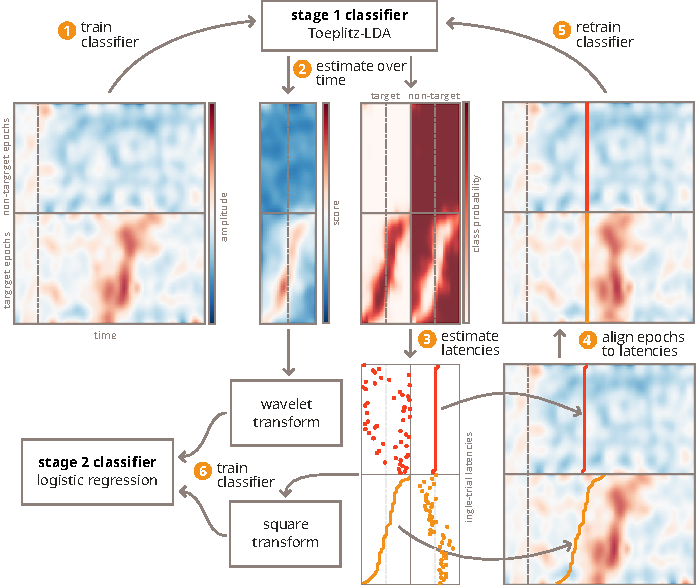
\includegraphics[width=.6\textwidth]{figures/covert/figure1.pdf}
%\end{frame}
%\begin{frame}
%  \frametitle{Aligned vs. non-aligned simulated data}
%\end{frame}
%\begin{frame}
%  \frametitle{Increase in gaze-independent decoding accuracy}
%\end{frame}
%
%\tocframe
%\section{\textbf{C3}: End-user case studies}
%\begin{frame}
%  \frametitle{Experimental setup}
%  \begin{itemize}
%    \item show setup
%    \item list participants
%  \end{itemize}
%\end{frame}
%\begin{frame}
%  \frametitle{Impaired visual skills}
%  show table
%\end{frame}
%\begin{frame}
%  \frametitle{Gaze tracking analysis}
%  highlight specific gaze case
%\end{frame}
%\begin{frame}
%  \frametitle{Usability}
%  how many achieved higher than chance?
%\end{frame}
%\section{Conclusion \& perspectives}


\end{document}
